\documentclass[oneside,11pt,letterpaper]{memoir}
\usepackage{forallxsyr}
\usepackage{fitch} % MR: this is adapted from Kl�wer's fitch style, Magnus adapted Selinger's for the book

\makeindex

\begin{document}\midsloppy



\frontmatter

%!TEX root = forallxsyr.tex
\thispagestyle{empty}


    \begin{tikzpicture}[remember picture, overlay]%
      \node [xshift=10.5cm,yshift=6.3cm] at (current page.south west) {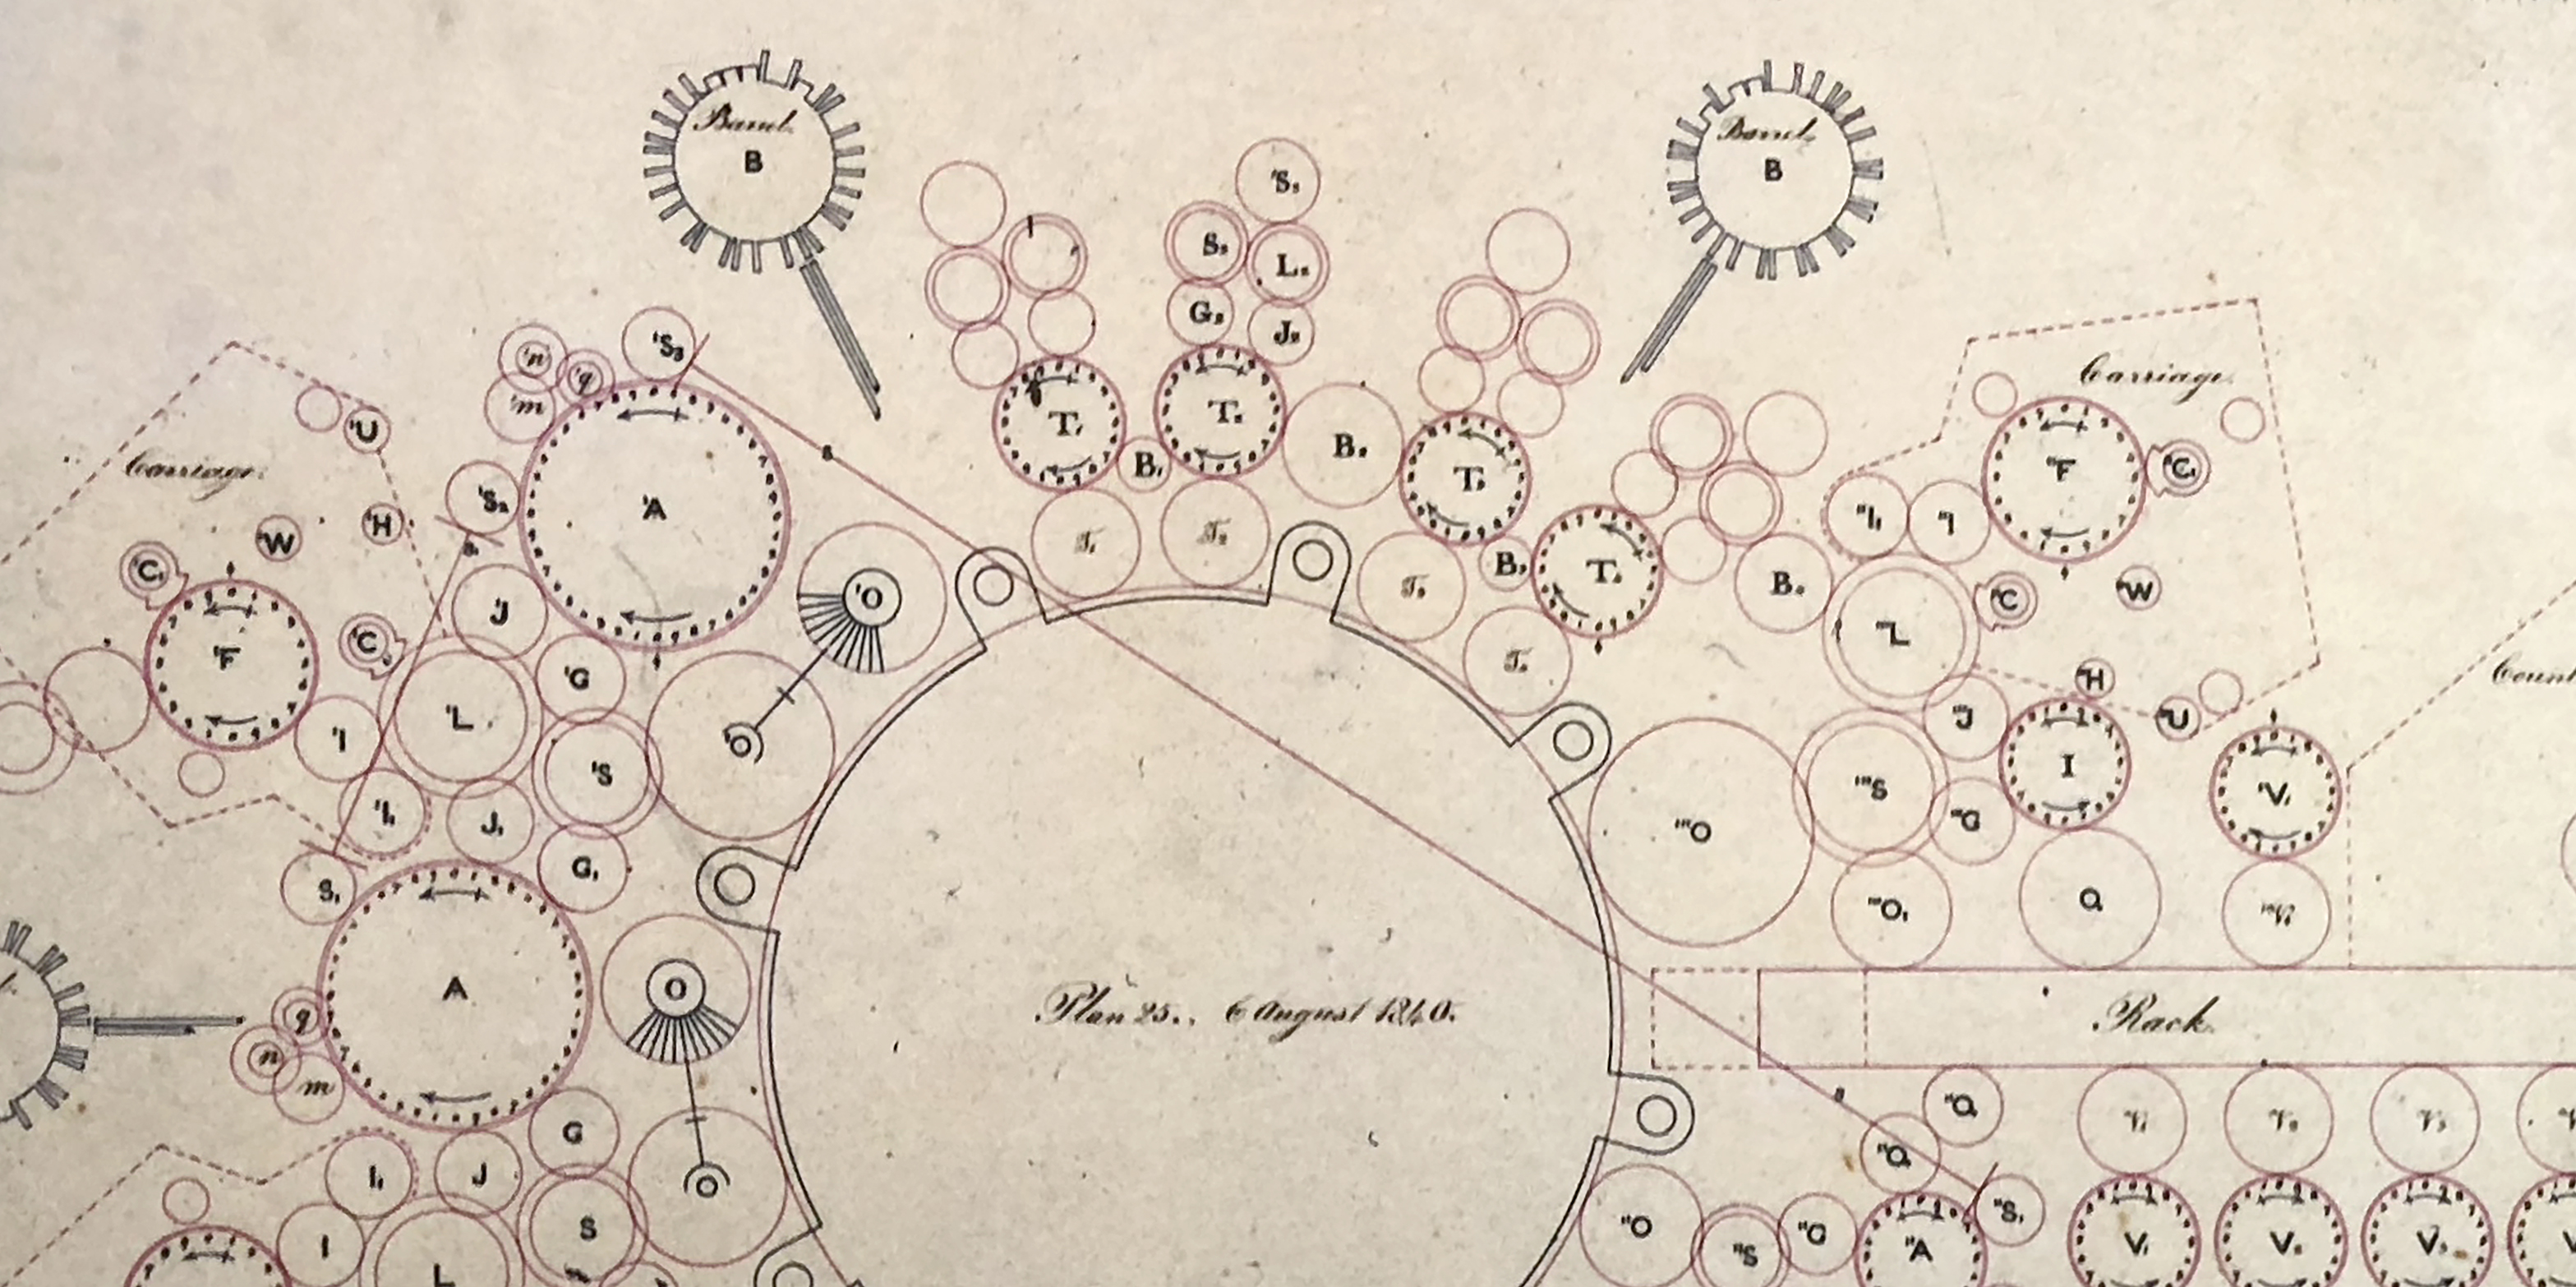
\includegraphics[scale=0.95]{cover-image.jpg}};%
    \end{tikzpicture}
    
\vspace{20pt}
    
\begin{center}
\fontsize{36pt}{36pt}\selectfont
  \textbf{forallx@syr}

\fontsize{24pt}{24pt}\selectfont
\vspace{1em}
\textit{An Introduction to\\ Formal Logic}


\vspace{40pt}

\fontsize{16pt}{18pt}\selectfont By P.~D. Magnus, Tim Button, and Michael Rieppel\\

\vspace{85pt}

\fontsize{20pt}{20pt}\selectfont
Spring 2021 Edition
\end{center}

\newpage


\noindent \small \copyright \ P.~D. Magnus, Tim Button, and Michael Rieppel, 2005-2021

\vspace{1ex}

\noindent This book is based on \href{http://www.homepages.ucl.ac.uk/~uctytbu/forallxcam.pdf}{\emph{forall x: Cambridge}}, by  \href{http://www.homepages.ucl.ac.uk/~uctytbu}{Tim Button}
(UCL), used under a \href{https://creativecommons.org/licenses/by/4.0/}{CC BY 4.0} license.  Button's book is in turn based on the original \href{https://www.fecundity.com/logic/}{\emph{forall x}}, by
\href{https://www.fecundity.com/job/}{P.D.\ Magnus} (SUNY Albany), used under a \href{https://creativecommons.org/licenses/by/4.0/}{CC BY 4.0} license.

\vspace{1ex}

\noindent The present text, \emph{forallx@syr}, was revised and expanded by \href{https://mrieppel.net/}{Michael Rieppel} (Syracuse University).  This work is licensed under a \href{https://creativecommons.org/licenses/by-sa/4.0/}{CC BY-SA 4.0} (Creative Commons Attribution-ShareAlike 4.0) license.  You are free to copy and redistribute the material in any medium or format, and  remix, transform, and build upon the material for any purpose, even commercially, under the following terms:
\begin{itemize}
\item Attribution -- You must give appropriate credit, provide a link to the license, and indicate if changes were made. You may do so in any reasonable manner, but not in any way that suggests the licensor endorses you or your use.

\item ShareAlike -- If you remix, transform, or build upon the material, you must distribute your contributions under the same license as the original.

\item No additional restrictions -- You may not apply legal terms or technological measures that legally restrict others from doing anything the license permits.
\end{itemize}

\vspace{1ex}
\noindent Cover Image: plan for Babbage's Analytical Engine (1840). Available at \href{https://commons.wikimedia.org/wiki/File:Babbage_Analytical_Engine_Plan_1840_CHM.agr.jpg}{Wikimedia Commons}.

\vspace{1ex}

\noindent The \LaTeX{} source for this book is available on GitHub at \href{https://github.com/mrieppel}{https://github.com/mrieppel}. 

\vspace{1ex}

\noindent The present version was released on \today.

\vspace{1ex}
\noindent Thanks to Yasmeen Hembree, Scott Looney, Ian York, and Yulun Zeng for spotting typos in earlier versions.

\newpage
\normalsize
\chapter*{Preface}

I first learned formal logic from Michael Byrd at UW-Madison, using Lemmon's  \emph{Beginning Logic}, and first taught logic in 2008 as a teaching assistant for Branden Fitelson at UC Berkeley, using Forbes' \emph{Modern Logic}.  When I started to develop my own logic course, I continued to use Forbes' book, which I liked for its thorough treatment of the three central components of an introductory logic class: symbolization, semantics, and natural deduction.  

However, over time I became dissatisfied with \emph{Modern Logic} for two reasons.  First, the Lemmon-style notation that it uses for natural deduction is much less accessible to beginners than the Fitch-style notation found in other texts.  And second, Oxford University Press started printing fewer copies of the book, making it rather expensive --- more expensive, at any rate, than I thought an introductory logic text should be.  By the time I began teaching at Syracuse in 2015, I therefore started listing Forbes' book only as a recommended text, and relied heavily on the detailed lecture notes I had put together over the years.

But in the longer term, I faced a choice: either select a new textbook, or transform my own notes into a book.  The open-source nature of Tim Button's \emph{forall x: Cambridge} offered me way to do both: I could take his already excellent text (which \emph{inter alia} included a Fitch-style deduction system) and supplement it with material of my own.  And so I've come to make my own addition to the ``groaning shelves'' of logic textbooks, to borrow Forbes' description --- though with electronic distribution, the groan has thankfully become more metaphorical. The main additions I've made to \emph{forall x: Cambridge} are the following:
\begin{itemize}
\item I've changed the first chapter to reflect my own introductory lecture, by e.g. elucidating the modal notion of validity using possible worlds, and emphasizing logic's focus on formal validity a bit more.
\item I've added more on the semantics of truth-functional and especially first-order logic, particularly as concerns the construction of countermodels.  
\item I've made some changes to set of natural deduction rules in both parts.
\item I've reordered the presentation of various topics and revised the practice problems.
\end{itemize}
Besides the obvious debt the present text owes to the \emph{forall x} editions that P.D. Magnus and Tim Button have so generously made available,  and to Forbes' \emph{Modern Logic}, I also draw on ideas I've picked up from Barwise and Etchemendy's \emph{Language, Proof, and Logic}, Belnap's \emph{The Art of Logic}, Goldfarb's \emph{Deductive Logic}, \emph{forall x: Calgary Remix}, and lecture notes by Branden Fitelson,  Daniel Warren, and John MacFarlane.





\newpage




\tableofcontents*

\newpage

\thispagestyle{empty}
\begin{quote}
``When you come to any passage you don't understand, \emph{read it again}: if you \emph{still} don't understand it, \emph{read it again}: if you fail, even after \emph{three} readings, very likely your brain is getting a little tired. In that case, put the book away, and take to other occupations, and next day, when you come to it fresh, you will very likely find that it is \emph{quite} easy.

``If possible, find some genial friend, who will read the book along with you, and will talk over the difficulties with you. \emph{Talking} is a wonderful smoother-over of difficulties. When I come upon anything --- in Logic or in any other hard subject --- that entirely puzzles me, I find it a capital plan to talk it over, \emph{aloud}, even when I am all alone.''

\begin{flushright} Lewis Carroll,  \emph{Symbolic Logic} (1897) \end{flushright}
\end{quote}



\mainmatter
%!TEX root = forallxsyr.tex
\chapter{What is Logic?}

\section{Arguments}\label{s:Arguments}


This book provides an introduction to logic.  But what is logic? This is a surprisingly difficult question, still debated by philosophers. But generally speaking, logic is about distinguishing \emph{valid} from \emph{invalid} arguments.

In everyday language, the word `argument' is often used to describe an activity that people engage in.   On twitter, or youtube, or the evening news, people often have heated disagreements, and you've probably had arguments like this with your family or friends.  Logicians tend to be a pretty sedate crowd, and they mean something very different by `argument'.  In logic, an argument is just a collection of statements.  More specifically:

\factoidbox{An \define{argument} is a collection of one or more \emph{statements}, exactly one of which is the argument's \emph{conclusion} and the rest of which are its \emph{premises}.}

\noindent Here is an example of an argument:

\begin{earg}
\item[\ex{exarg1}]All rabbits are mammals.
\item[] Bugs Bunny is a rabbit.
\item[] $\therefore$ Bugs Bunny is a mammal.
\end{earg}

This argument consists of three statements.  One of them is argument's conclusion, which we indicated by the three dots $\therefore$ read as ``therefore.'' The rest are its premises.  This argument has two premises, but arguments can have any number of premises (though, again, only one conclusion).

Notice that our logician's definition of an argument is very permissive. Consider the following:
	\begin{earg}
		\item[] There is a bassoon-playing dragon in the \emph{Cathedra Romana}.
		\item[] $\therefore$ Salvador Dali was a poker player.
	\end{earg}
We have a premise and a conclusion, and so we have an argument. Admittedly, it is a \emph{terrible} argument. But it is still an argument.  

Here's another argument, one that's not as obviously terrible:


\begin{earg}
\item[\ex{exarg2}]All rabbits are mammals.
\item[] Winnie the Pooh is a mammal.
\item[] $\therefore$ Winnie the Pooh is a rabbit.
\end{earg}

In this case the premises at least involve the same concepts as the conclusion.  But this argument still isn't as good as \eref{exarg1} from earlier: unlike the earlier example, this argument isn't valid --- its conclusion doesn't follow from its premises.  But what exactly does validity, or ``following from,'' consist in?  What's wrong with argument \eref{exarg2} as compared to \eref{exarg1}?

One thing that's bad about the second argument is that its conclusion is false: Pooh isn't a rabbit, he's a bear!  But that isn't what distinguishes valid from invalid arguments, because there are valid arguments with false conclusions, and invalid arguments with true conclusions:


\begin{earg}
\item[\ex{exarg3}]All rabbits are birds.
\item[] Winnie the Pooh is a rabbit.
\item[] $\therefore$ Winnie the Pooh is a bird.
\end{earg}

\begin{earg}
\item[\ex{exarg4}]All rabbits are mammals
\item[] Bugs Bunny is a mammal.
\item[] $\therefore$ Bugs Bunny is a rabbit.
\end{earg}



The first of these is valid, but has a false conclusion.  And the second has a true conclusion, as well as true premises, but it still isn't valid because its conclusion doesn't follow from its premises.  

Validity isn't about whether the premises or conclusion are in fact true.  It rather has to do with the \emph{relationship} between the premises and the conclusion.  When we ask about validity we want to know whether, if all the premises were true, the conclusion would also \emph{have to be true}.  Put another way:


\factoidbox{
An argument is \define{valid} if and only if it is \emph{impossible} for all of its premises to be true but its conclusion to be false.}

 
 \noindent Let's unpack some of the concepts involved in the two definitions we've encountered a little bit more.


\practiceproblems

As you've seen, we always put the conclusion at the end of an argument and indicate it using the three ``therefore dots'' $\therefore$.  Informally presented arguments don't always have the conclusion at the end, however --- it can appear at the beginning, or even in the middle.  In each of the following arguments, highlight the phrase which expresses the conclusion:

\begin{earg}
	\item It is sunny. So I should take my sunglasses.
	\item It must have been sunny. I did wear my sunglasses, after all.
	\item No one but you has had their hands in the cookie-jar. And the scene of the crime is littered with cookie-crumbs. You're the culprit!
	\item Miss Scarlett and Professor Plum were in the study at the time of the murder. And Reverend Green had the candlestick in the ballroom, and we know that there is no blood on his hands. Hence Colonel Mustard did it in the kitchen with the lead-piping. Recall, after all, that the gun had not been fired.
\end{earg}


 
 \section{Background Concepts}\label{s:Background}
 
 First, we said that an argument is a collection of \define{statements}.  Statements are sentences that are either true or false.  Truth and falsity are called \define{truth-values}.  The truth-value of a statement is determined by what the world is like: a statement like `Syracuse is in New York State' describes the world as being a certain way, and is true or false depending on whether the world is that way.   As the ancient philosopher (and logician!) Aristotle put it in his book \emph{Metaphysics}:

\begin{quote}
``To say of what is that it is not, or of what is not that it is, is false, while to say of what is that it is, and of what is not that it is not, is true.'' (1011b25)
\end{quote}

It's important to notice that not all English sentences count as statements in this sense.  For example, none of the following sentences can be assessed as true or false:

\begin{ebullet}
\item Welcome to the Syracuse Airport! 
\item Please have your ID ready.
\item Are there any liquids in your bag?
\end{ebullet}

A sentence like `please have your ID ready' isn't meant to describe the world, but to ask someone to do something.  Similarly, `Welcome to Syracuse Airport' is just a greeting, and isn't meant to offer an accurate or inaccurate description of the world.  And although the answer to the last question on this list has a truth-value, the question itself doesn't.  In general, things like greetings, requests, orders, and questions don't have truth-values, and therefore don't count as statements and cannot be premises or conclusions of arguments.  Though it's important to keep this point in mind, moving forward we'll generally use the words ``statement'' and ``sentence'' interchangeably.


Next, notice that because a statement's truth value depends on what the world is like, its truth-value could have been different if the world had been different.  For example, the sentence`Rieppel is a philosopher' is in fact true, but if I had taken up a different career it would have been false.  Conversely, `Rieppel is a professional juggler' is false, but if I had gone to juggling school instead of continuing with philosophy, it would have been true.   

Philosophers often invoke the notion of a \define{possible world} in this connection.  The idea is that besides the actual world, there are various other possible worlds, other ways things could have been --- alternative histories, or alternative universes, if you like.  `Rieppel is a professional juggler' is false at the actual world, but it is true at various other possible worlds.  Sentences like this, which are true in some possible worlds but not others, are said to be contingent.

Other sentences are not contingent.  For example, `Syracuse either is or is not in New York State' isn't just true at the actual world, it's true at \emph{every} possible world, that is, it's a necessary truth.  Mathematical truths are another example: $2+2 = 4$ is again true in every possible world, and therefore a necessary truth. At the other extreme, a sentence like `Syracuse both is and is not in New York State' is false in every possible world, or necessarily false.  

Returning to arguments, you can think of the notion of validity in terms of possible worlds too.  We said that an argument is valid just in case it's \emph{impossible} for all of its premises to be true but it's conclusion false.  Put in terms of possible worlds, we can say that an argument is valid if and only if there is \emph{no possible world} where all  its premises are true but its conclusion is false.  Equivalently put: its conclusion is true at every possible world at which all its premises are true. So again, whether an argument is valid or not doesn't depend on whether its premises and conclusion are in fact true or false.  It's about the connection between them --- whether it is \emph{possible} for the conclusion to be false while all the premises are true.


There are various logical concepts that we'll encounter in this class that involve the notions of necessity and possibility, besides validity.  Here are some of them:


\factoidbox{
\begin{itemize}

\item A sentence is \define{contingent} if and only if it is possible for it to be true, and also possible for it to be false.

\item A sentence is a \define{necessary truth} if and only if it is not possible for it to be false.

\item A sentence is a \define{necessary falsehood} if and only if it is not possible for it to be true.

\item Two sentences are \define{contradictory} if and only if they necessarily have opposite truth values.

\item Two sentence are \define{equivalent} if and only if they necessarily have the same truth value.

\item A collection of sentences is \define{jointly consistent} if and only if it is possible for all of them to be true together, and \define{jointly inconsistent} otherwise.


\end{itemize}
} 
Notice that these concepts apply to different things. Whereas the first three concern properties of single sentences, the next two concern relations between two sentences, and the last ones properties of collections of sentences.  Validity is again slightly different, because it is a property had (or lacked) by only those collections of sentences that also have a designated conclusion.    

\practiceproblems
\problempart
\label{pr.EnglishTautology}
For each of the following: is it necessarily true, necessarily false, or contingent?
\begin{earg}
\item Caesar crossed the Rubicon.
\item Someone once crossed the Rubicon.
\item No one has ever crossed the Rubicon.
\item If Caesar crossed the Rubicon, then someone has.
\item Even though Caesar crossed the Rubicon, no one has ever crossed the Rubicon.
\item If anyone has ever crossed the Rubicon, it was Caesar.
\end{earg}

\problempart
\label{pr.MartianGiraffes}
Consider the following sentences:

	\begin{ebullet}
		\item[G1.] There are at least four giraffes at the wild animal park.
		\item[G2.] There are exactly seven gorillas at the wild animal park.
		\item[G3.] There are not more than two martians at the wild animal park.
		\item[G4.] Every giraffe at the wild animal park is a martian.
	\end{ebullet}
	
Now, for each of the following, determine if the sentences in question are jointly consistent or jointly inconsistent:

\begin{earg}
\item G2, G3, and G4
\item G1, G3, and G4
\item G1, G2, and G4
\item G1, G2, and G3
\end{earg}


\problempart
Could there be:
	\begin{earg}
		\item Jointly consistent sentences, one of which is necessarily false?
		\item Jointly consistent sentences, one of which is a necessary truth?
		\item Jointly inconsistent sentences, one of which is a necessary truth?
	\end{earg}
In each case: if so, give an example; if not, explain why not.




\section{Good and Bad Arguments}\label{s:GoodBadArg}

Being valid is certainly one thing that makes for a good argument, intuitively speaking.  But there's more to being a good argument than that.

First off, if an argument has an obviously false premise, then even if it is valid, it remains of limited interest because it doesn't establish its conclusion.  By contrast, if an argument is valid and all of its premises are true, then we know that its conclusion must be true too.  Arguments of this latter sort are said to be \emph{sound}:

\factoidbox{
An argument is \define{sound} if and only it (i) is valid, and (ii) has premises that are in fact true.
}

Arguments are generally intended to be not just valid, but sound.  So if you're faced with an argument, in a philosophy class or elsewhere, whose conclusion you want to resist, you have two options: you can either try to show that the argument is not valid, or you can try to show that one of its premises is false.  What you can't do is accept it as valid, and concede that its premises are true, but still reject the conclusion as false.

Although its very important in practice to determine whether or not the premises of an argument are true, it is (for the most part) not the job of logic to do this.  The job of logic is just to determine whether or not an argument is valid.  The task of determining whether the argument's premises are in fact true (and the argument sound) is usually best left to experts in the relevant field: biologists, philosophers, historians, physicists, economists, or whomever.

A second way in which validity is not all there is to good argumentation comes out if you consider the following:
	\begin{earg}
		\item[] In January 2015, it snowed in Syracuse.
		\item[] In January 2016, it snowed in Syracuse.
		\item[] In January 2017, it snowed in Syracuse.
		\item[] In January 2018, it snowed in Syracuse.
		\item[] In January 2019, it snowed in Syracuse.
	\item[So:] It snows every January in Syracuse.
\end{earg}

This argument generalizes from observations about several past cases to a conclusion about all cases. The argument isn't valid, because even if it snowed in many recent years, that doesn't mean it's impossible for it not to snow in some future year.  The argument could be made stronger by adding additional premises, about other snowy Syracuse Januaries in the past. But however many premises of this sort we add, the argument will remain invalid.

That doesn't mean that it's a bad argument.  Arguments like this one are called \emph{inductive} arguments, and they are often used legitimately and with great success in science and everyday life.  In this book, we shall set aside (entirely) the difficult question of what makes for a good inductive argument.  What logic studies is the different notion of \emph{deductive} validity --- where truth of the premises has to \emph{guarantee} truth of the conclusion --- and this will be the focus of our concern.

\practiceproblems

Here are some exercises to test your understanding of deductive validity and related concepts we've discussed.  For these questions, you don't need to worry about the distinction between validity and ``validity in virtue of logical form.'' That is, you can just assume the definition of validity we gave in \S\ref{s:Arguments} above.\\


\problempart  Which of the following arguments are valid? Which are invalid?

\begin{enumerate}
\item \begin{earg}
\item[] Socrates is a man.
\item []All men are carrots.
\item[$\therefore$]Socrates is a carrot.
\end{earg}

\item \begin{earg}
\item[] Abe Lincoln was either born in Illinois or he was once president.
\item[] Abe Lincoln was never president.
\item[$\therefore$] Abe Lincoln was born in Illinois.
\end{earg}

\item \begin{earg}
\item[] If I pull the trigger, Abe Lincoln will die.
\item[] I do not pull the trigger.
\item[$\therefore$] Abe Lincoln will not die.
\end{earg}

\item \begin{earg}
\item[] Abe Lincoln was either from France or from Luxemborg.
\item[] Abe Lincoln was not from Luxemborg.
\item[$\therefore$] Abe Lincoln was from France.
\end{earg}

\item \begin{earg}
\item[] If the world were to end today, then I would not need to get up tomorrow morning.
\item[] I will need to get up tomorrow morning.
\item[$\therefore$] The world will not end today.
\end{earg}

\item \begin{earg}
\item[] Joe is now 19 years old.
\item[] Joe is now 87 years old.
\item[$\therefore$] Bob is now 20 years old.
\end{earg}

\end{enumerate}

\problempart
Could there be:
	\begin{earg}
		\item A valid argument that has one false premise and one true premise?
		\item A valid argument that has only false premises but a true conclusion?
		\item A valid argument with only false premises and a false conclusion?
		\item A valid argument with only true premise but a false conclusion?
		\item An invalid argument with only true premises and a true conclusion?
		\item An invalid argument with only false premises but a true conclusion?
		\item A sound argument with a false conclusion?
		\item A sound argument with at least one false premise?
		\item An invalid argument that can be made valid by the addition of a new premise?
		\item A valid argument that can be made invalid by the addition of a new premise?
		\item A valid argument, the conclusion of which is necessarily false?
		\item An invalid argument, the conclusion of which is necessarily true?
		\item A valid argument whose premises are jointly inconsistent?
		\item A valid argument with only one premise?
	\end{earg}
In each case: if so, give an example; if not, explain why not. 




\section{Formal Validity}\label{s:FormalValidity}

There's one last complication we have to address before setting out on our investigation of logic.  Consider the following arguments:

	\begin{earg}
		\item[\ex{exarg5}] The sculpture is green all over.
		\item[] $\therefore$ The sculpture is not red all over. 
	\end{earg}
	
	\begin{earg}
		\item[\ex{exarg6}]  Reihan is a bachelor.
		\item[] $\therefore$ Reihan is not married.
	\end{earg}
	
In both cases it is impossible for the premise to be true and the conclusion false: if something's green all over it can't be any other color, and being unmarried is part of what it is to be a bachelor.  Both arguments are therefore valid. 

But there's an important difference between valid arguments like these and one like the following:

	\begin{earg}
		\item[\ex{exarg8}] Jenny is either happy or sad.
		\item[] Jenny is not happy.
		\item[] $\therefore$ Jenny is sad.
	\end{earg}

\noindent This argument is also valid, but there's more.  It has a special structure, or logical form, that we might represent as follows:


	\begin{earg}
		\item[] $A$ or $B$
		\item[] not-$A$
		\item[] $\therefore$ $B$
	\end{earg}

\noindent This is an excellent form for an argument to have, because any argument of this form will be valid, no matter what sentences occur in place of $A$ and $B$! Or consider our Bugs Bunny argument, which has the structure represented to the right:



\begin{multicols}{2}
	
\begin{earg}
\item[\eref{exarg1}]All rabbits are mammals.
\item[] Bugs Bunny is a rabbit.
\item[] $\therefore$ Bugs Bunny is a mammal.
\end{earg}
	
\columnbreak

\begin{earg}
	\item[] All $F$ are $G$
	\item[] $a$ is $F$
	\item[] $\therefore$ $a$ is $G$
\end{earg}

\end{multicols}


\noindent Again, any argument of this form will be valid, no matter what predicates we put in for $F$ and $G$ or what name we put in for $a$.


We can put the general point by saying that arguments like \eref{exarg8} and  \eref{exarg1} are valid simply \emph{in virtue of their logical form}.  They each exhibit a structure which renders any argument with that structure valid.  By contrast, arguments \eref{exarg5}  and \eref{exarg6}, though valid, are not valid in virtue of their logical form.  For example, here's another argument that has the same form as \eref{exarg6} but that isn't valid:


\begin{multicols}{2}

\begin{earg}
\item[] Reihan is a runner.
\item[] $\therefore$ Reihan is not married.
\end{earg}

\columnbreak

\begin{earg}
\item[] $a$ is $F$
\item[] $\therefore$ $a$ is not-$G$.
\end{earg}

\end{multicols}

\noindent What made argument \eref{exarg6} valid wasn't its logical form, but the connection between the  meanings of the specific words `bachelor' and `married' that occur in its premise and conclusion.  Logic is all about patterns, and only cares about \emph{formally} valid arguments like \eref{exarg1} and \eref{exarg8}, not arguments like \eref{exarg5} and \eref{exarg6} that are valid for reasons other than their logical form. 

\section{A Look Ahead}

Due to logic's concern with form, we will approach the task of distinguishing valid from invalid arguments in an indirect way. We will first introduce a formal language in which we can symbolize English arguments, thereby letting us represent their logical forms.  We will then give a precise definition of validity for arguments cast in this formal notation, which will in turn give us our indirect means of distinguishing valid from invalid arguments in English: an English argument is formally valid if it can be symbolized as a valid argument in our formal notation.

In fact, we will study two systems of logic, involving two different formal languages. These systems will differ in what words they treat as \emph{logical constants}, i.e. what words they treat as indicative of logically significant structure.  The first system we will study is \emph{Truth-Functional Logic} (or TFL).  It will let us represent the structure of arguments like \eref{exarg8} via the symbolization to the right:

\begin{multicols}{2}

	\begin{earg}
		\item[\eref{exarg8}] Jenny is either happy or sad.
		\item[] Jenny is not happy.
		\item[] $\therefore$ Jenny is sad.
	\end{earg}

\columnbreak

	\begin{earg}
		\item[] $(A \eor B)$
		\item[] $\enot A$
		\item[] $\therefore$ $B$
	\end{earg}

\end{multicols}

\noindent This language will treats words like `either \ldots or' and `not' as logical constants, and will use upper-case letters to represent complete sentences.

The second system of logic we will study is \emph{first-order logic} (or FOL).  It will let us represent the structure of things like the Bugs Bunny argument via the symbolization to the right:


\begin{multicols}{2}

\begin{earg}
\item[\eref{exarg1}]All rabbits are mammals.
\item[] Bugs Bunny is a rabbit.
\item[] $\therefore$ Bugs Bunny is a mammal.
\end{earg}

\columnbreak

	\begin{earg}
		\item[] $\forall x(Fx \eif Gx)$
		\item[] $Fa$
		\item[] $\therefore$ $Ga$
	\end{earg}

\end{multicols}

\noindent This system extends truth-functional logic by additionally treating words like `all' as logical constants, and using upper- and lower-case letters to represent English predicates and names, respectively.\footnote{At this point you might be wondering why logicians treat some words (like `either \ldots or', `not', and `all') as logical constants, but not other words (like `happy' or `bachelor').  This is a difficult philosophical question about logic that we won't get into here.  If you're interested, check out the \emph{Stanford Encyclopedia of Philosophy's} entries on \href{http://plato.stanford.edu/entries/logical-constants/}{Logical Constants} and  \href{http://plato.stanford.edu/entries/logical-consequence/}{Logical Consequence}.} With this short preview out of the way, let's get started with logic! 




%\problempart We've seen that arguments can be valid despite having false premises or false conclusions, and invalid despite having true premises or true conclusions.  Give your own examples of these:
%
%\begin{enumerate}
%\item A valid argument with: 
%\begin{itemize}
%\item true conclusion and only true premises
%\item true conclusion and at least one false premise
%\item false conclusion and at least one false premise
%\end{itemize}
%
%\item An invalid argument with: 
%\begin{itemize}
%\item true conclusion and only true premises
%\item true conclusion and at least one false premise
%\item false conclusion and at least one false premise
%\item false conclusion and only true premises\footnote{Notice: there are invalid arguments like this, but there can't be valid arguments of this sort!}
%\end{itemize}
%\end{enumerate}

%!TEX root = forallxsyr.tex
\part{Truth Functional Logic}
\chapter{Symbolization in TFL}



\section{Atomic sentences}

In this chapter, we'll look at how to symbolize English arguments in the language of \emph{truth-functional logic} (or TFL), thereby revealing their truth-functional logical structure, or form.\footnote{What does ``truth-functional'' mean?  We'll get to that in the next chapter, on the semantics of TFL.}  Here is an example of a symbolization in TFL:


	\begin{earg}
		\item[\ex{exarg1}] It is raining outside.
		\item[] If it is raining outside, then Jenny is miserable.
		\item[] $\therefore$ Jenny is miserable.
	\end{earg}


\begin{multicols}{2}

	\begin{earg}
		\item[] $A$
		\item[] If $A$, then $C$
		\item[] $\therefore$ $C$
	\end{earg}

\columnbreak

	\begin{earg}
		\item[] $A$
		\item[] $(A \rightarrow C)$
		\item[] $\therefore$ $C$
	\end{earg}


\end{multicols}


In symbolizing this argument, I began by replacing  \emph{subsentences} of larger sentences with uppercase letters. For example, `it is raining outside' is a subsentence of the complex sentence `If it is raining outside, then Jenny is miserable', and we replaced this subsentence with the letter `$A$'.  Similarly, we used `$C$' to symbolize the subsentence `Jenny is miserable'.

Our artificial language, TFL, uses uppercase letters as its \define{atomic sentences}. These will be the basic building blocks, or ``atoms,'' out of which more complex TFL sentences are built.  There are only twenty-six letters of the alphabet, but in principle there is no limit to the number of atomic sentences that we might want to consider. By adding numerical subscripts to letters, we obtain as many atomic sentences as we need.  So the following all count as atomic sentences of TFL:

	$$A, P, P_1, P_2, A_{234}$$

To indicate which atomic sentence of TFL is being used to represent which English sentence, we provide a \define{symbolization key}, such as the following:

	\begin{ekey}
		\item[A] It is raining outside
		\item[C] Jenny is miserable
	\end{ekey}

Doing this does \emph{not} fix this symbolization \emph{once and for all}. We are just saying that, for the time being, we will use the atomic TFL sentence `$A$' to symbolize the English sentence `It is raining outside', and `$C$' to symbolize `Jenny is miserable'. Later, when we are dealing with different sentences or different arguments, we can provide a new symbolization key that associates these atomic TFL sentences with different English sentences.


It is important to recognize that whatever internal structure an English sentence might have is lost if it is symbolized by an atomic sentence of TFL. From the point of view of TFL, an atomic sentence has no internal (or ``subatomic'') structure. It can be used to build more complex sentences, but it cannot be taken apart.

For this reason, English sentences that have an internal logical structure to them, like the conditional `If it's raining outside, then Jenny is miserable', should not be symbolized using atomic sentences of TFL.  If we just symbolized this sentence as `$P$', for example, our symbolization would obscure the fact that it has the form of an `if \ldots then \ldots' statement, and that it contains subsentences that also occur on their own as premise and conclusion in our argument \eref{exarg1} above. We would thefore miss out on the logical form in virtue of which argument \eref{exarg1} is valid.

For this reason we have to symbolize logically complex sentences of English via complex (i.e. non-atomic) sentence of TFL, in this case `$(A \rightarrow C)$'.  Complex sentences of TFL are built up by combining atomic sentences with \emph{connectives}.


%\section{Connectives}\label{s:TFLConnectives}

TFL connectives will be used to symbolize English connectives like `if \ldots then', `or' and `not'.  Just as these English connectives can be applied to sentences to form new, bigger sentences, so TFL connectives can be applied to atomic sentences to build larger, complex sentences of TFL.  in total, there are five connectives in TFL. This table summarizes them, and gives you a rough indication of their meaning:


	\begin{table}[h]
	\center
	\begin{tabular}{l l l}

	\textbf{symbol}&\textbf{name}&\textbf{rough meaning}\\
	\hline
	\enot&negation&`It is not the case that$\ldots$'\\
	\eand&conjunction&`Both$\ldots$\ and $\ldots$'\\
	\eor&disjunction&`Either$\ldots$\ or $\ldots$'\\
	\eif&conditional&`If $\ldots$\ then $\ldots$'\\
	\eiff&biconditional&`$\ldots$ if and only if $\ldots$'\\

	\end{tabular}
	\end{table}

For the remainder of this chapter, we have two main objectives, a practical one and a technical one.  The first, practical objective is to learn how to symbolize logically complex English sentences using our TFL connectives.  The second, more technical objective will be to give a precise grammar, or syntax, for the language of TFL, which explains exactly how TFL connectives combine with atomic sentences to produce complex TFL sentences.  We'll turn to this technical task later, after we've gotten some practice using the language of TFL to symbolize English sentences.

\section{Negation}

Consider how we might symbolize these sentences:

	\begin{earg}
	\item[\ex{not1}] Mary is in Barcelona.
	\item[\ex{not2}] It is not the case that Mary is in Barcelona.
	\item[\ex{not3}] Mary is not in Barcelona.
	\end{earg}

In order to symbolize \eref{not1}, we will need an atomic sentence. We might offer this symbolization key:

	\begin{ekey}
		\item[B] Mary is in Barcelona.
	\end{ekey}

Since \eref{not2} is obviously related to \eref{not1}, we do not want to symbolize it with a completely different sentence, say `$A$'. Roughly, sentence \eref{not2} means something like `It is not the case that B'. In order to symbolize this, we need a symbol for negation. We will use `\enot'. Now we can symbolize \eref{not2} with `$\enot B$'.

Sentence \eref{not3} also contains the word `not'. And it is obviously equivalent to \eref{not2}. As such, we can also symbolize it with `$\enot B$'.
\factoidbox{
A sentence can be symbolized as $\enot\meta{\varphi}$ if it can be paraphrased in English as `It is not the case that \meta{\varphi}'.
}

Here's another example:

	\begin{earg}
		\item[\ex{not4}] The widget can be replaced.
		\item[\ex{not5}] The widget is irreplaceable.
		\item[\ex{not5b}] The widget is not irreplaceable.
	\end{earg}

Let's use the following symbolization key:

	\begin{ekey}
		\item[R] The widget is replaceable
	\end{ekey}

Sentence \eref{not4} can then be symbolized by `$R$'. Next, \eref{not5} says the widget is irreplaceable, which means that it is not the case that the widget is replaceable. So even though \eref{not5} does not contain the word `not', we can still symbolize it as `$\enot R$'.  Sentence \eref{not5b} can be paraphrased as `It is not the case that the widget is irreplaceable.' Which can again be paraphrased as `It is not the case that it is not the case that the widget is replaceable'. So we can symbolize this with the TFL sentence `$\enot\enot R$'.

At this point you might be wondering: don't double negatives cancel out, so that `$\enot\enot R$' is equivalent to plain `$R$'? We'll get into meaning, or semantics, of TFL sentences in the next chapter, but the quick answer is that, yes, these are equivalent, and \eref{not5b} \emph{could} also be symbolized as `$R$'.  Still, `$\enot \enot R$' is the \emph{preferred} symbolization, since it represents more of the logical structure implicit in the English sentence \eref{not5b}.

Some care is needed when handling negations. Consider:
	\begin{earg}
		\item[\ex{not6}] Jane is happy.
		\item[\ex{not7}] Jane is unhappy.
	\end{earg}
If we let `$H$' symbolize  `Jane is happy', we can symbolize \eref{not6} as `$H$'. However, it would be a mistake to symbolize \eref{not7} with `$\enot{H}$'. Sentence \eref{not7} does not mean the same thing as `It is not the case that Jane is happy'. Jane might be neither happy nor unhappy; she might be in a state of blank indifference. In order to symbolize \eref{not7}, then, we would need a new atomic sentence of TFL.

\section{Conjunction}\label{s:ConnectiveConjunction}

Consider the sentence:

	\begin{earg}
		\item[\ex{and3}]Adam is athletic, and Barbara is athletic.
	\end{earg}

We will need separate atomic sentences to symbolize the two subsentences that occur in \eref{and3}.

	\begin{ekey}
		\item[A] Adam is athletic.
		\item[B] Barbara is athletic.
	\end{ekey}

We will use `\eand' to symbolize `and', and thus symbolize \eref{and3} as `$(A\eand B)$'. This connective is called \define{conjunction}. We also say that `$A$' and `$B$' are the two \define{conjuncts} of the conjunction `$(A \eand B)$'.

There are few things to notice about conjunction.  First, in English the word `and' doesn't always conjoin two sentences:

	\begin{earg}
		\item[\ex{and4}]Barbara is athletic and energetic.
		\item[\ex{and5}]Barbara and Adam are both athletic.
	\end{earg}

In \eref{and4} the word `and' conjoins two adjectives, rather than two sentences.  But it can be paraphrased as `Barbara is athletic and Barbara is energetic' where `and' now does conjoin two complete sentences.  So if we use `$E$' symbolize `Barbara is energetic', we can symbolize the entire sentence as `$(B\eand E)$'.  In sentence \eref{and5}, `and' conjoins two names.  Again, though, this can be paraphrased in terms of a conjunction of two sentences, as `Barbara is athletic and Adam is athletic', and can therefore be symbolized as `$(B \land A)$'.\footnote{Some care is needed with this.  Not \emph{all} sentences where `and' conjoins two names can be paraphrased in a way where `and' conjoins two sentences.  For example, `Barbara and Adam carried the piano upstairs' may not mean the same as `Barbara carried the piano upstairs and Adam carried the piano upstairs', since the latter (but not the former) is compatible with them each carrying it individually rather than together. }

Second, conjunction can be expressed in English using words other than `and':

	\begin{earg}
	\item[\ex{and6}]Although Barbara is energetic, she is not athletic.
	\item[\ex{and7}]Adam is athletic, but Barbara is not.
	\end{earg}

In \eref{and6}, the word `although' sets up a contrast between the first part of the sentence and the second part. Nevertheless, the sentence tells us both that Barbara is energetic and that she is not athletic.  So we can symbolize it as a conjunction:

\begin{ekey}
		\item[B] Barbara is athletic.
		\item[E] Barbara is energetic.
\end{ekey}

\begin{itemize}
\item[] Symbolization of \eref{and6}: $(E \eand \enot B)$
\end{itemize}

Of course we have lost all sorts of nuance in this symbolization. There is a distinct difference in tone between the English sentence \eref{and6} and `Both Barbara is energetic and it is not the case that Barbara is athletic'. TFL does not (and cannot) preserve these nuances, however, and so we do not attend to them when symbolizing English into TFL.  Notice also that in the symbolization key we replaced the pronoun `she' with `Barbara', since it might otherwise be unclear who `she' is meant to refer to.  In general: always use names in place of pronouns in your symbolization key!


Sentence \eref{and7} raises similar issues. The word `but' sets up a contrast between the two parts of the sentence, but this is not something that TFL can deal with. We can paraphrase the sentence as `\emph{Both} Adam is athletic, \emph{and} Barbara is not athletic'.  Notice that the second conjunct involves a negation as well.  Using the sentence letters already introduced, we can symbolize \eref{and7} as `$(A \eand \enot B)$'.


There are other words besides `although' and `but' that can be used to express conjunction.  For example, `Barbara is energetic, however she is not athletic' and `Barbara is energetic despite not being athletic' expresses the same conjunctive claim as sentence \eref{and6} from above, and get symbolized using the same TFL sentence. In general, the symbolization guideline for conjunction is:

	\factoidbox{
		A sentence can be symbolized as $(\meta{\varphi}\eand\meta{\psi})$ if (nuance aside) it can be paraphrased in English as `Both \meta{\varphi} and \meta{\psi}'.
}

You might be wondering why we always put \emph{brackets} around the conjunctions. The reason can be brought out by thinking about negation interacts with conjunction. Consider:

	\begin{earg}
		\item[\ex{negcon1}] You will not get both soup and salad.
		\item[\ex{negcon2}] You will not get soup but you will get salad.
	\end{earg}

Sentence \eref{negcon1} can be paraphrased as `It is not the case that: both you will get soup and you will get salad'. Using the following symbolization key:
	\begin{ekey}
		\item[S_1] You get soup.
		\item[S_2] You get salad.
	\end{ekey}
we would symbolize `both you will get soup and you will get salad' as `$(S_1 \eand S_2)$'. To symbolize the whole of sentence \eref{negcon1}, then, we negate this, giving us `$\enot (S_1 \eand S_2)$'. Sentence \eref{negcon2}, on the other hand, gets symbolized as a conjunction whose first conjunct is negated `$(\enot S_1 \eand S_2)$'.

These English sentences are very different, and their symbolizations differ accordingly. In one of them, the entire conjunction is negated. In the other, just one conjunct is negated. Brackets help us to keep track of things like the \emph{scope} of the negation: whether it applies to the whole conjunction, or just to the first conjunct.

\section{Disjunction}\label{s:Disjunction}
Consider these sentences:
	\begin{earg}
		\item[\ex{or1}]Either Denison will play golf with me, or he will watch movies.
		\item[\ex{or2}]Either Denison or Ellery will play golf with me.
	\end{earg}
We can use the following symbolization key for these sentences (notice that we, as always, replace pronouns with names):
	\begin{ekey}
		\item[D] Denison will play golf with me.
		\item[E] Ellery will play golf with me.
		\item[M] Denison will watch movies.
	\end{ekey}
Sentence \eref{or1} is and `either \ldots or' statement, and gets symbolized as `$(D \eor M)$'. The connective is called \define{disjunction}. We also say that `$D$' and `$M$' are the \define{disjuncts} of the disjunction `$(D \eor M)$'.

Sentence \eref{or2} is only slightly more complicated.  Here `or' occurs between two names rather than two complete sentences. However, we can paraphrase sentence \eref{or2} as `Either Denison will play golf with me, or Ellery will play golf with me' where `or' now connects two complete sentences. So we can symbolize it as `$(D \eor E)$'.
	\factoidbox{
		A sentence can be symbolized as $(\meta{\varphi}\eor\meta{\psi})$ if it can be paraphrased in English as `Either \meta{\varphi} or \meta{\psi}.'
	}


Sometimes in English, the word `or' excludes the possibility that both disjuncts are true. This is called an \define{exclusive or}.  An \emph{exclusive or} is  intended when it says, on a restaurant menu, `Entrees come with either soup or salad': you may have soup; you may have salad; but, if you want \emph{both} soup \emph{and} salad, then you have to pay extra.  At other times, the word `or' allows for the possibility that both disjuncts might be true. This is probably the case with sentence \eref{or2}, above: I might play golf with Denison, with Ellery, or with both Denison and Ellery. Sentence \eref{or2} merely says that I will play with \emph{at least} one of them. This is an \define{inclusive or}.

Importantly, the TFL symbol `\eor' expresses \emph{inclusive or}.  Whenever you see the English words `either \ldots or' in this book, you can assume that the inclusive sense is intended, and symbolize such sentences using `$\eor$'.  When an exclusive sense is  intended, we will always add an explicit `but not both', as in:
	\begin{earg}
		\item[\ex{or.xor}] The entree will come with either soup or salad, but not both.
	\end{earg}
Using `$S_1$' for `the entree will come with soup' and `$S_2$' for `the entree will come with salad', we can symbolize \eref{or.xor} as `$((S_1 \eor S_2) \eand \enot (S_1 \eand S_2))$'.  So although the TFL symbol `\eor' always symbolizes \emph{inclusive or}, we can symbolize an \emph{exclusive or} in {TFL}. We just have to use a few other TFL symbols in addition to `$\eor$'!


There are some futher interesting interactions between disjunction and negation that we should attend to. Consider the following:

	\begin{earg}
		\item[\ex{or3}] Either Barbara will not get soup, or she will not get salad.
		\item[\ex{or4}] Barbara will get neither soup nor salad.
	\end{earg}
Sentence \eref{or3} can be paraphrased as: `\emph{Either} it is not the case that Barbara will get soup, \emph{or} it is not the case that Barbara will get salad'.  Using the following symbolization key:

	\begin{ekey}
		\item[P] Barbara will get soup.
		\item[D] Barbara will get salad.
	\end{ekey}
we can symbolize \eref{or3} as $(\enot P \eor \enot D)$.  This has the form of a disjunction both disjuncts of which are negated.  Sentence \eref{or4} has a different structure. It can be paraphrased as, `\emph{It is not the case that}: either Barbara will get soup or Barbara will get salad'. Since this negates the entire disjunction, we symbolize sentence \eref{or4} as `$\enot (P \eor D)$'.  This differs from our symbolization of \eref{or3}, as it should given that the two English sentences mean different things.

You may have noticed that \eref{or3} means the same thing as `Barbara will not get both soup and salad.'  The latter can be symbolized as a negated conjunction, `$\enot(P \eand D)$'.  Since `$\enot(P \eand D)$' symbolizes an English sentence that's equivalent to \eref{or3}, and \eref{or3} is symbolized as `$(\enot P \eor \enot D)$', we can conclude that the TFL sentences `$\enot(P \eand D)$'  and `$(\enot P \eor \enot D)$' are themselves equivalent.

Similarly, \eref{or4} means the same as `Barbara will not get soup and Barbara will not get salad', which can be symbolized as a conjunction of two negations `$(\enot P \eand \enot D)$'.  So again, since `$(\enot P \eand \enot D)$' symbolizes an English sentence that's equivalent to \eref{or4}, and \eref{or4} is symbolized as `$\enot (P \eor D)$', we can conclude that these two TFL sentences are themselves equivalent.  What we've discovered are:

\factoidbox{\define{DeMorgan's Laws}:
\begin{itemize}
\item[] $\enot(\meta{\varphi} \eor \meta{\psi})$ is equivalent to $(\enot \meta{\varphi} \eand \enot \meta{\psi})$
\item[] $\enot(\meta{\varphi} \eand \meta{\psi})$ is equivalent to $(\enot \meta{\varphi} \eor \enot \meta{\psi})$
\end{itemize}}

\noindent These  laws are named after Augustus DeMorgan who first explicitly formulated them in the nineteenth century.  These laws will stay with us throughout our study of logic, and we will see how to prove that these equivalences hold in the next chapter.\footnote{It is noteworthy that these equivalences only hold in TFL given that `$\eor$' expresses inclusive disjunction.  The fact that the corresponding English sentences are also intuitively equivalent again shows that English `or' often expresses inclusive disjunction.}


\section{Conditional}
Consider these sentences:
	\begin{earg}
		\item[\ex{if0}] If Jean is in Paris, then Jean is in France.
		\item[\ex{if1}] Jean is in France if Jean is in Paris.
		\item[\ex{if2}] Jean is in France only if Jean is in Paris.
	\end{earg}
Let's use the following symbolization key:
	\begin{ekey}
		\item[P] Jean is in Paris.
		\item[F] Jean is in France
	\end{ekey}
Sentence \eref{if0} is roughly of this form: `if P, then F'. We will use the symbol `\eif' to symbolize the English `if\ldots, then\ldots' structure. So we symbolize sentence \ref{if1} by `$(P\eif F)$'. The connective is called \define{the conditional}. Here, `$P$' is called the \define{antecedent} of the conditional `$(P \eif F)$', and `$F$' is called the \define{consequent}.

Sentence \eref{if1} looks different from \eref{if0} since the word `if' occurs in the middle of the sentence rather than at the beginning.  But clearly \eref{if1} it is equivalent to \eref{if0}, so we can also symbolize it as `$(P \eif F)$'.  In general, the `if'-clause of an English conditional always introduces the \emph{antecedent}, whether or not it occurs first in the English sentence, with the rest of the sentence functioning as the \emph{consequent}.


Sentence \eref{if2} is also a conditional. Since the word `if' appears in the second half of the sentence, it might be tempting to symbolize this in the same way as sentence \eref{if1}, as `$(P \eif F)$'. But that would be a mistake. My knowledge of geography tells me that sentence \eref{if1} is unproblematically true: there is no way for Jean to be in Paris that doesn't involve Jean being in France. But sentence \eref{if2} is not so straightforward: were  Jean in Marseilles, Lyons, or Toulouse, Jean would be in France without being in Paris, thereby rendering sentence \eref{if2} false. Since geography alone dictates the truth of sentence \eref{if1}, whereas travel plans (say) are needed to know the truth of sentence \eref{if2}, they must mean different things, and \eref{if2} can't be symbolized as `$(P \eif F)$.

The moral is that `only if' means something very different from plain `if'.  The `if'-clause of a conditional introduces a \define{Sufficient Condition}: \eref{if0} and \eref{if1} say that Jean's being in Paris is \emph{sufficient for} his being in France (which is unproblematically true).  `Only if', by contrast, introduces a \define{Necessary Condition}: sentence \eref{if2} claims that Jean's being in Paris \emph{is necessary for} his being in France (which is likely false, since there are other ways to be in France). In TFL, the antecedent \meta{\varphi} of a conditional $(\meta{\varphi} \eif \meta{\psi})$ always indicates the sufficient condition, whereas the consequent \meta{\psi} indicates the the necessary condition.  Since Jean's being in Paris is claimed as a necessary condition in \eref{if2}, this sentence is symbolized as `$(F \eif P)$'.  In general, whereas `if' introduces the antecedent of a conditional (the sufficient condition), `only if' introduces the consequent (the necessary condition).  So our symbolization guidelines for conditionals are:

	\factoidbox{
		A sentence can be symbolized as $(\meta{\varphi} \eif \meta{\psi})$ if it can be paraphrased in English as `If \meta{\varphi}, then \meta{\psi}', or as `\meta{\psi} if \meta{\varphi}', or as `\meta{\varphi} only if \meta{\psi}'.
	}

The fact that \eref{if0} is symbolized as the conditional `$(P \eif F)$' means that this `if\ldots then' statement can also be paraphrased as an `only if' statement: `Jean is in Paris only if Jean is in France'.  That's intuitively correct: since his being in Paris is sufficient for his being in France, it's also true that his being in France is necessary for his being in Paris.

This connection between conditionals and necessary and sufficient conditions also indicates that the conditional can represent many English constructions that don't involve the word `if' at all.  The following are all ways of saying that Jean's being in Paris is \emph{sufficient for} his being in France:
\begin{earg}
\item[\ex{ifsc1}]  Jean is in France \emph{provided that} he is in Paris.
\item[\ex{ifsc2}] Jean is in France \emph{as long as} he is in Paris.
\item[\ex{ifsc3}] Jean is in France \emph{whenever} he is in Paris.
\item[\ex{ifsc4}] For Jean to be in France \emph{it is enough that} he be in Paris.
\item[\ex{ifsc5}] For Jean to be in France \emph{it is sufficient that} he be in Paris.
\end{earg}
So all of these can be symbolized as `$(P \eif F)$'.  Similarly, the following are all ways of saying that his being in France is \emph{necessary for} his being in Paris:
\begin{earg}
\item[\ex{ifnc1}] Jean's being in Paris is \emph{contingent on} his being in France.
\item[\ex{ifnc1}]  For Jean to be in Paris  \emph{it is required that} he be in France.
\item[\ex{ifnc1}]  For Jean to be in Paris  \emph{it is necessary that} he be in France.
\end{earg}
So these can all be symbolized as `$(P \eif F)$' as well.

One final point: it is important to bear in mind that the connective `\eif' tells us only that if the antecedent is true, then the consequent is true. It says nothing about a \emph{causal} or \emph{explanatory} connection between two events (for example), though English conditionals often carry such a suggestion. In fact, we lose a huge amount when we use `$\eif$' to symbolize English conditionals. We will look more closely at the discrepancies between English `if\ldots then' and the TFL connective `\eif' in \S\ref{s:TFLConditional}.

\section{Biconditional}
Consider the following sentence:

	\begin{earg}
		%\item[\ex{iff1}] Shergar is a horse only if it he is a mammal
		%\item[\ex{iff2}] Shergar is a horse if he is a mammal
		\item[\ex{iff3}] Shergar is a horse if and only if he is a mammal
	\end{earg}
Let's use the following symbolization key:
	\begin{ekey}
		\item[H] Shergar is a horse
		\item[M] Shergar is a mammal
	\end{ekey}
Sentence \ref{iff3} can be paraphrased as `Shergar is a horse if he is a mammal, and Shergar is a horse only if Shergar is a mammal'. This is just the conjunction of two conditionals we already know how to symbolize.   So we can symbolize it as `$((H \eif M) \eand (M \eif H))$'. We call this a \define{biconditional}, because it amounts to stating both directions of the conditional.  That is, \eref{iff3} says (falsely, as it happens) that Shergar's being a mammal is both necessary and sufficient for his being a horse.

We could treat every biconditional this way, as a conjunction of two conditionals. So, just as we do not need a new TFL symbol to deal with \emph{exclusive or}, we do not really need a new TFL symbol to deal with biconditionals. However, since biconditionals occur a lot in logic an philosophy, we'll use the dedicated connective `\eiff' to symbolize them. We can then can symbolize sentence \ref{iff3} with the TFL sentence `$(H \eiff M)$'.

Since `if and only if' gets used so much in logic and philosophy, it is often abbreviated with a single, snappy word, `iff'. I shall follow this practice. So `if' with only \emph{one} `f' is the English conditional. But `iff' with \emph{two} `f's is the English biconditional. Armed with this we can say:
	\factoidbox{
		A sentence can be symbolized as $(\meta{\varphi} \eiff \meta{\psi})$ if it can be paraphrased in English as `\meta{\varphi} if and only if \meta{\psi}', that is, `\meta{\varphi} iff \meta{\psi}'.
	}

Another way to express a biconditional relationship in English is with the words `just in case', as in:
\begin{earg}
\item[\ex{iff2}] The triangle is equilateral just in case all of its sides have the same length.
\end{earg}
This says that the triangle's having sides of the same length is both necessary and sufficient for it's being equilateral. If we use `$E$' for `the triangle is equilateral' and `$S$' for `the triangle's sides have the same length', it can be symbolized as the biconditional `$(E \eiff S)$'.


%A word of caution. Ordinary speakers of English often use `if \ldots, then\ldots' when they really mean to use something more like `\ldots if and only if \ldots'. Perhaps your parents told you: `if you don't eat your greens, you won't get any dessert'. Suppose you ate your greens, but that your parents then refused to give you any dessert, on the grounds that they were only committed to the \emph{conditional} (`if you get dessert, then you will have eaten your greens'), rather than the biconditional (`you get dessert iff you eat your greens'). Well, a tantrum would rightly ensue. So, be aware of this when interpreting people; but in your own writing, make sure to use the biconditional iff you mean to.


\section{`Unless'}
We have now seen all of the connectives of TFL. We can use them together to symbolize many kinds of sentences. But some cases are harder than others. And a typically nasty case is the English-language connective `unless':
\begin{earg}
\item[\ex{unless1}] Unless you wear a jacket, you will catch a cold.
\item[\ex{unless2}] You will catch a cold unless you wear a jacket.
\end{earg}
These two sentences are clearly equivalent. Let's use the following symbolization key:
	\begin{ekey}
		\item[J] You will wear a jacket.
		\item[D] You will catch a cold.
	\end{ekey}
Both sentences mean that if you do not wear a jacket, then you will catch a cold. So we could symbolize them as `$(\enot J \eif D)$'.   In general, you can think of `unless' as having the meaning `if not', so sentences of the form `Unless \meta{\varphi}, \meta{\psi}' or `\meta{\psi} unless \meta{\varphi}' mean `If not \meta{\varphi}, then \meta{\psi}' or again, `\meta{\psi} if not \meta{\varphi}', and can be symbolized as $(\enot \meta{\varphi} \eif \meta{\psi})$.


As we shall see in the next chapter, in TFL `$(\enot J \eif D)$' is equivalent to the disjunction `$(J \eor D)$'.  So this is another way to symbolize \eref{unless1} or \eref{unless2}.  And that makes some sense: intuitively they do say that either you will wear a jacket, or you will catch a cold.

So we can use the following guideline:
	\factoidbox{
		If a sentence can be paraphrased as `Unless \meta{\varphi}, \meta{\psi}' or `\meta{\psi} unless \meta{\varphi}', then it can be symbolized as $(\enot\meta{\varphi} \eif \meta{\psi})$, or simply $(\meta{\varphi}\eor\meta{\psi})$.
	}

There is a little complication. `Unless' can be symbolized as a conditional or an inclusive disjuntion. But ordinary speakers of English often use `unless' to mean something more like the biconditional, or like exclusive disjunction. Suppose I say: `I will go running unless it rains'. I probably mean something like `I will go running if and only if it does not rain' (i.e.\ the biconditional), or  `either I will go running or it will rain, but not both' (i.e.\ exclusive disjunction). However, in this book we'll always use `unless' in the strict sense in which it can be symbolized using a conditional or an inclusive disjunction.  (As it happens, our guideline here is also the one used on the LSAT.)


\practiceproblems
\problempart Using the symbolization key given, symbolize each English sentence in TFL.\label{pr.monkeysuits}
	\begin{ekey}
		\item[M] Those creatures are men in suits.
		\item[C] Those creatures are chimpanzees.
		\item[G] Those creatures are gorillas.
	\end{ekey}
\begin{earg}
\item Those creatures are not men in suits.
\item Those creatures are men in suits, or they are not.
\item Those creatures are either gorillas or chimpanzees.
\item Those creatures are neither gorillas nor chimpanzees.
\item If those creatures are chimpanzees, then they are neither gorillas nor men in suits.
\item Unless those creatures are men in suits, they are either chimpanzees or they are gorillas.
\end{earg}

\problempart Using the symbolization key given, symbolize each English sentence in TFL.
\begin{ekey}
\item[A] Mister Ace was murdered.
\item[B] The butler did it.
\item[C] The cook did it.
\item[D] The Duchess is lying.
\item[E] Mister Edge was murdered.
\item[F] The murder weapon was a frying pan.
\end{ekey}
\begin{earg}
\item Either Mister Ace or Mister Edge was murdered.
\item If Mister Ace was murdered, then the cook did it.
\item If Mister Edge was murdered, then the cook did not do it.
\item Either the butler did it, or the Duchess is lying.
\item The cook did it only if the Duchess is lying.
\item If the murder weapon was a frying pan, then the culprit must have been the cook.
\item If the murder weapon was not a frying pan, then the culprit was either the cook or the butler.
\item Mister Ace was murdered if and only if Mister Edge was not murdered.
\item The Duchess is lying, unless it was Mister Edge who was murdered.
\item If Mister Ace was murdered, he was done in with a frying pan.
\item Since the cook did it, the butler did not.
\item Of course the Duchess is lying!
\end{earg}
\problempart Using the symbolization key given, symbolize each English sentence in TFL.\label{pr.avacareer}
	\begin{ekey}
		\item[E_1] Ava is an electrician.
		\item[E_2] Harrison is an electrician.
		\item[F_1] Ava is a firefighter.
		\item[F_2] Harrison is a firefighter.
		\item[S_1] Ava is satisfied with her career.
		\item[S_2] Harrison is satisfied with his career.
	\end{ekey}
\begin{earg}
\item Ava and Harrison are both electricians.
\item If Ava is a firefighter, then she is satisfied with her career.
\item Ava is a firefighter, unless she is an electrician.
\item Harrison is an unsatisfied electrician.
\item Neither Ava nor Harrison is an electrician.
\item Both Ava and Harrison are electricians, but neither of them find it satisfying.
\item Harrison is satisfied only if he is a firefighter.
\item If Ava is not an electrician, then neither is Harrison, but if she is, then he is too.
\item Ava is satisfied with her career if and only if Harrison is not satisfied with his.
\item If Harrison is both an electrician and a firefighter, then he must be satisfied with his work.
\item It cannot be that Harrison is both an electrician and a firefighter.
\item Harrison and Ava are both firefighters if and only if neither of them is an electrician.
\end{earg}

\problempart
\label{pr.spies}
Give a symbolization key and symbolize the following English sentences in TFL.
\begin{earg}
\item Alice and Bob are both spies.
\item If either Alice or Bob is a spy, then the code has been broken.
\item If neither Alice nor Bob is a spy, then the code remains unbroken.
\item The German embassy will be in an uproar, unless someone has broken the code.
\item Either the code has been broken or it has not, but the German embassy will be in an uproar regardless.
\item Either Alice or Bob is a spy, but not both.
\end{earg}

\problempart Give a symbolization key and symbolize the following English sentences in TFL.
\begin{earg}
\item If there is food to be found in the pridelands, then Rafiki will talk about squashed bananas.
\item Rafiki will talk about squashed bananas unless Simba is alive.
\item Rafiki will either talk about squashed bananas or he won't, but there is food to be found in the pridelands regardless.
\item Scar will remain as king if and only if there is food to be found in the pridelands.
\item If Simba is alive, then Scar will not remain as king.
\end{earg}

\problempart
For each argument, write a symbolization key and symbolize all of the sentences of the argument in TFL.
\begin{earg}
\item If Dorothy plays the piano in the morning, then Roger wakes up cranky. Dorothy plays piano in the morning unless she is distracted. So if Roger does not wake up cranky, then Dorothy must be distracted.
\item It will either rain or snow on Tuesday. If it rains, Neville will be sad. If it snows, Neville will be cold. Therefore, Neville will either be sad or cold on Tuesday.
\item If Zoog remembered to do his chores, then things are clean but not neat. If he forgot, then things are neat but not clean. Therefore, things are either neat or clean; but not both.
\end{earg}

\problempart
We symbolized \emph{exclusive or}, or \emph{xor}, using `$\eor$', `$\eand$', and `$\enot$'. How could you symbolize an \emph{xor} using only two connectives? Hint: think about how you might use DeMorgan's Laws to eliminate one of the connectives in your symbolization.



\section{The Syntax of TFL}\label{s:TFLSyntax}

In the course of learning to symbolize English sentences in TFL, we've gotten a pretty good intuitive sense of how to build up complex TFL sentences from atomic ones using our five connectives.  But as we move ahead, it will be necessary for us to be a bit more precise about the structure of our logical language.  Because just as not every string of English words counts as a grammatical English sentence (e.g. `shelf on book red lies' is just gibberish), so not every string of symbols counts as grammatical, or well-formed sentence of TFL.

We have seen that there are three kinds of symbols in TFL:
\begin{center}
\begin{tabular}{l l}
Atomic sentences: & $A,B,C,\ldots,Z, \ldots, A_1, B_1,Z_1,A_2,A_{25},J_{375},\ldots$\\
\\
Connectives: & $\enot,\eand,\eor,\eif,\eiff$\\
\\
Brackets: &( , )\\
\end{tabular}
\end{center}

This constitutes the \define{Lexicon} of TFL.  Now define an \define{expression of TFL} to be any string of symbols of TFL.  That is: write down any sequence of symbols from the lexicon of TFL, in any order, and you have an expression of TFL.

Strings like `$(A \leftarrow B)$' or `$(p \eor C)$' or `$\enot (\varphi \eand A)$' are not expressions of TFL because they contain symbols like `$\leftarrow$' (leftward arrows) `$p$' (lowercase letters) and `$\varphi$' (Greek letters) that are not even in the Lexicon of TFL.  On the other hand, `$(A \eand B)$' is an expression of TFL, and so are `$(\enot)A\rightarrow)$' and `$\lnot)(\eor()\eand(\enot\enot())((B$'. However, whereas the first of these expressions also counts as a \emph{sentence} of TFL, the rest are just \emph{gibberish}. What we want are some rules to tell us precisely which TFL expressions count as sentences.


Obviously, individual atomic sentences like `$A$' and `$G_{13}$' should count as sentences. We can form further sentences out of these by using the various connectives. Using negation, we can get `$\enot A$' and `$\enot G_{13}$'. Using conjunction, we can get `$(A \eand G_{13})$', `$(G_{13} \eand A)$', `$(A \eand A)$', and `$(G_{13} \eand G_{13})$'. We could also apply negation repeatedly to get sentences like `$\enot \enot A$' and `$\enot \enot \enot A$', or apply negation to one of our conjunctions to get sentences like `$\enot(A \eand G_{13})$' and `$\enot(G_{13} \eand \enot G_{13})$'. There are infinitely many possible combinations, even starting with just these two sentence letters.  And of course there are infinitely many sentence letters. So there is no point in trying to list all of the sentences of TFL one by one.

Instead, we will describe the process by which sentences can be \emph{constructed}. Consider negation: given any sentence \meta{\varphi} of TFL, putting a negation in front of it gives us a sentence $\enot\meta{\varphi}$ .
We can say similar things for each of the other connectives. For instance, if \meta{\varphi} and \meta{\psi} are sentences of TFL, then $(\meta{\varphi}\eand\meta{\psi})$ is a sentence of TFL.  (What's up with the funny Greek letters, which are \emph{not} in the lexicon of TFL?  We'll get to that in \S\ref{s:TFLMetavariables} below.)


Providing clauses like this for all of the connectives, we arrive at the following \define{Syntax}, or formal definition of what counts as a  \define{sentence of TFL}:
	\factoidbox{
	\define{The Syntax of TFL:}
	\begin{enumerate}
		\item Every atomic sentence is a sentence.
		\item If \meta{\varphi} is a sentence, then $\enot\meta{\varphi}$ is a sentence.
		\item If \meta{\varphi} and \meta{\psi} are sentences, then $(\meta{\varphi}\eand\meta{\psi})$ is a sentence.
		\item If \meta{\varphi} and \meta{\psi} are sentences, then $(\meta{\varphi}\eor\meta{\psi})$ is a sentence.
		\item If \meta{\varphi} and \meta{\psi} are sentences, then $(\meta{\varphi}\eif\meta{\psi})$ is a sentence.
		\item If \meta{\varphi} and \meta{\psi} are sentences, then $(\meta{\varphi}\eiff\meta{\psi})$ is a sentence.
		\item Nothing else is a sentence.
	\end{enumerate}
	}
Definitions like this are called \emph{recursive}. Recursive definitions begin with some list of base elements (in this case, atomic sentences), and then present ways to generate indefinitely many more elements by compounding together previously generated elements.  We can then determine if any given TFL expression counts as a sentence by checking whether it can be generated by applying these recursive rules of syntax.



For example, suppose we want to know whether or not `$\enot \enot D$' is a sentence of TFL. Looking at clause 2 of the definition, we know that `$\enot \enot D$' is a sentence \emph{if} `$\enot D$' is a sentence. So now we need to ask whether or not `$\enot D$' is a sentence. Again looking at  clause 2 of the definition, `$\enot D$' is a sentence \emph{if} `$D$' is. And `$D$' is an atomic sentence of TFL, so we know that `$D$' is a sentence by the clause 1 of the definition. So by applying the clauses of our definition repeatedly, we see that our original sentence `$\enot \enot D$' can be generated by applying the rules of our syntax to atomic sentences, and thus counts as a TFL sentence.


Next, consider a more complex example: `$\enot (P \eand \enot (\enot Q \eor R))$'. Looking at clause 2 of the definition, this is a sentence if `$(P \eand \enot (\enot Q \eor R))$' is. And by clause 3 the latter is a sentence if \emph{both} `$P$' \emph{and} `$\enot (\enot Q \eor R)$' are sentences. The former is an atomic sentence, and the latter is a sentence if `$(\enot Q \eor R)$' is a sentence. Looking at clause 4, we see this is a sentence if both `$\enot Q$' and `$R$' are sentences. And both are!  So we've shown that the expression we started with is indeed a sentence.

Notice that negation differs from our other operators.  It attaches to a \emph{single} sentence to form a new sentence, and is therefore called a \define{Unary Operator}.  By contrast, the other operators all operate on \emph{pairs} of sentences to form new sentences, and are therefore called \define{Binary Operators}.

Our syntactic rules tell us that any sentence formed by applying a binary operator to a pair of sentences must be enclosed by parentheses.  For example, when putting `$S$' and `$R$' together using a conjunction, the resulting sentence `$(S \eand R)$' must have brackets around it.  So `$S \eand R$' is not technically a sentence of TFL, but a mere expression.  This is \emph{not} the case for negation, however!  Putting a negation in front of a sentence never requires adding parentheses.  So `$\enot \enot D$' and `$\enot (S \eand R)$' are well-formed sentences, but `$(\enot (\enot (D)))$' or `$(\enot (S \eand R))$' are not sentences.  (We'll return to the rationale behind these bracketing rules in \S \ref{s:TFLBracketing} below.)

\subsection{Some Syntactic Notions}\label{s:TFLSyntacticNotions}



Ultimately, every TFL sentence is constructed nicely out of atomic sentences on the basis of our syntactic rules. When we are dealing with any complex (i.e. non-atomic) sentence, we can see that there must be some connective that was introduced \emph{most recently} when constructing that sentence. We call that the \define{main operator} of the sentence:

\factoidbox{The \define{Main Operator} of a complex TFL sentence is the one that was introduced \emph{most recently} in the process of constructing that sentence.
}

In the case of `$\enot\enot D$', the main operator is the very first `$\enot$' sign. In the case of `$((\enot E \eor F) \eif \enot G)$', the main operator is `$\eif$' because the last step in constructing this sentence is to connect `$(\enot E \eor F)$' and `$\enot G$' using `$\eif$' (and putting brackets around the result).  One can visually represent the process in which a sentence is constructed from its parts via  a \define{syntactic tree} for the sentence.  For example, the syntactic tree for `$((\enot E \eor F) \eif \enot G)$' looks like this:\\

\Tree [.{$((\enot E \eor F) \eif \enot G)$} [.{$(\enot E \eor F)$}  [.{$\enot E$} {$\enot$} {$E$} ] {$\eor$} {$F$} ] {$\eif$} [.{$\enot G$} {$\enot$} {$G$} ] ]  \\

\noindent This shows that `$((\enot E \eor F) \eif \enot G)$' was constructed by connecting `$(\enot E \eor F)$' and `$\enot G$' using `$\eif$', and `$(\enot E \eor F)$' was in turn constructed by connecting `$\enot E$' and `$F$' using `$\eor$', and `$\enot E$' was constructed by putting `$\enot$' in front of `$E$', and so on. If we represent the construction process in terms of a tree structure like this, then the main operator of a sentence is whichever operator occurs on a branch of its own at the \emph{first level} below the sentence as a whole (which again, in this case, is `$\eif$').


The syntactic structure of sentences in TFL also allows us to give a formal definition of the \emph{scope} of a negation (mentioned in \S\ref{s:ConnectiveConjunction}). The scope of a `$\enot$' in a given sentence is whatever subsentence of that sentence has `$\enot$' as its main logical operator. For example, consider the complex TFL sentence:
$$(\enot (R \eand B) \eiff Q)$$
This was constructed by putting a biconditional between `$\enot (R \eand B)$' and `$Q$' . So `$\enot (R \eand B)$' is a \emph{subsentence} of the sentence as a whole.  And the main logical operator for this subsentence is `$\enot$'. So the scope of the negation in `$(\enot (R \eand B) \eiff Q)$' is just `$\enot(R \eand B)$'. More generally:
	\factoidbox{The \define{scope} of any connective in a sentence is the subsentence for which that connective is the main logical operator.}
So again in the case of `$(\enot (R \eand B) \eiff Q)$', the scope of `$\eiff$' is the sentence as a whole (since it is the main operator of the whole sentence), and the scope of `$\eand$' is `$(R \eand B)$', since $(R \eand B)$ is the subsentence of which `$\eand$' is the main  operator.

\subsection{Bracketing}\label{s:TFLBracketing}

As mentioned in \S\ref{s:ConnectiveConjunction} and \S\ref{s:TFLSyntax} above, brackets are an important part of the syntax of TFL.  This is because they demarcate the scope of connectives.  For example, there is an important difference between `$\enot (P \eand Q)$' and `$(\enot P \eand Q)$'.  In the case of  `$\enot (P \eand Q)$' the scope of the negation operator is the whole sentence, that is, it is the main operator of the sentence and it serves to negate the entire conjunction it is attached to. In the case of `$(\enot P \eand Q)$', the scope of the negation is just the subsentence `$\enot P$', and the main operator of the sentence as a whole is `$\eand$'.

Strictly speaking, therefore, a string like `$\enot P \eand Q$' is \emph{not} a sentence of TFL, but a mere expression, because it is missing brackets.  As things stand, it is not clear where in `$\enot P \eand Q$' the brackets are supposed to go, that is, whether it is supposed to be a negated conjunction, i.e. `$\enot (P \eand Q)$', or rather a conjunction with a negated left conjunct, i.e.  `$(\enot P \eand Q)$'.  When working with TFL, however, it will make our lives easier if we are sometimes a little less strict. So, here are some convenient conventions.

First,  we'll allow ourselves to omit the \emph{outermost} brackets on a sentence. Thus we allow ourselves to write `$Q \eand R$' instead of `$(Q \eand R)$'. However, we have to put the brackets back in when we want to embed this sentence into another, larger sentence!  So we cannot write `$P \rightarrow Q \eand R$', but must write $P \rightarrow (Q \eand R)$' instead.  With this convention in place, something like `$\enot P \eand Q$' can now be interpreted as missing its outermost parentheses, and thus being a shorthand for `$(\enot P \eand Q)$' rather than `$\enot (P \eand Q)$'.

Second, it can be a bit painful to stare at long sentences with many nested pairs of brackets. To make things a bit easier on the eyes, we will allow ourselves to use square brackets, `[' and `]', instead of rounded ones. So there is no logical difference between `$(P\eor Q)$' and `$[P\eor Q]$', for example. Combining this convention with the first one, we can rewrite the unwieldy sentence:
$$(((H \eif I) \eor (I \eif H)) \eand (J \eor K))$$
more simply as follows:
$$\bigl[(H \eif I) \eor (I \eif H)\bigr] \eand (J \eor K)$$
The scope of each connective is now much more visually apparent.

\subsection{Metalanguage and Metavariables}\label{s:TFLMetavariables}

Our recursive definition of TFL sentences included clauses like the following:
\begin{enumerate}
\item[3.] If \meta{\varphi} and \meta{\psi} are sentences, then $(\meta{\varphi}\eand\meta{\psi})$ is a sentence.
\end{enumerate}
But notice that `$(\meta{\varphi} \eand \meta{\psi})$' is \emph{not} a sentence of TFL.  In fact, it isn't even an expression of TFL!  After all, it includes Greek letters, and these are not among the symbols that constitute the the lexicon of TFL.  Atomic TFL sentences are just ordinary uppercase roman letters (possibly subscripted) like `$A$' or `$B$' or `$S_{21}$', not Greek letters.  So what's going on in our recursive clauses?

The answer is that in these clauses, we are using Greek letters as \emph{variables} that ``range over'' arbitrary expressions of TFL.  Consider how, in a math class, you might explain to someone that if $m$ and $n$ are any two positive integers, it holds that $m + n \geq m$.  In this case we are using `$m$' and `$n$' as variables that range over arbitrary positive integers,  and saying that $m + n \geq m$ holds no matter what positive integers $m$  and $n$ are.  %On the other hand, if the variables were allowed to range over \emph{all} integers, positive and negative,  the claim $m + n \geq m$ would not longer hold --- now $m$ might be $2$ and $n$ might be ${-3}$, in which case $m+n \ngeq m$.

In the same way, we are here using Greek letters as variables, except that we are using them as variables that range over arbitrary expressions in the language of TFL (rather than over integers, say).  The language of TFL has been the object of our study for the past several sections, and we therefore call it the \define{Object Language}.  But we have been conducting our discussion of TFL in English, so English is our \define{Metalanguage}: it is the language in which we talk about the object language.\footnote{Of course these notions aren't fixed.  If we had been discussing the syntax of Korean, say, rather than TFL, then our metalanguage would still have been English, but our object language would have been Korean.}
For this reason, variables like `$\meta{\varphi}$' and `$\meta{\psi}$' are called \define{Metavariables}: they form part of our metalanguage, English, and they range over arbitrary expressions in our object language, TFL.  But again, these metavariables are \emph{only} part of our metalanguage, and not themselves included in the object language TFL.


	\factoidbox{
		Greek letters $\meta{\varphi}$, \meta{\psi}, \meta{\chi} etc. are \define{metavariables} in our \define{metalanguage}, used to talk about arbitrary expressions of TFL.  Roman letters $A, B, C \ldots$ etc. are atomic sentences of our \define{object language} TFL .}

So what clause 3 in our definition says is that if $\meta{\varphi}$ and $\meta{\psi}$ are any arbitrary sentences of TFL, then the result of writing whatever $\meta{\varphi}$ is, followed by `$\eand$', followed by whatever \meta{\psi} is, and enclosing the result in parentheses, produces a sentence of TFL.  For example, if \meta{\varphi} is the TFL sentence `$\enot D$' and \meta{\psi} is the TFL sentence `$(S \rightarrow T)$', then clause 3 tells us that `$(\enot D \eand (S \rightarrow T))$' is a sentence of TFL.  But again, the string of symbols `$(\meta{\varphi} \eand \meta{\psi})$' is not itself a sentence (nor even an expression) of TFL.

\practiceproblems
\problempart
\label{pr.wiffTFL}
For each of the following: (a) Is it a sentence of TFL, strictly speaking? (b) Is it a sentence of TFL, allowing for our relaxed bracketing conventions?
\begin{earg}
\item $(A)$
\item $J_{374} \eor \enot J_{374}$
\item $\enot \enot \enot \enot F$
\item $\enot \enot \enot (\enot F)$
\item $\enot \eand S$
\item $(G \eand \enot G)$
\item $(A \eif (A \eand \enot F)) \eor (D \eiff E)$
\item $(A \eand (B \eand ((C \eand D) \eand E)))$
\item $[(Z \eiff S) \eif W] \eand [J \eor X]$
\item $(F \eiff \enot D \eif J) \eor (C \eand D)$
\end{earg}

\problempart
What is the main operator in each of the following?  And what are the scopes of the other operators in these sentences?

\begin{earg}
\item $\enot(A \eif \enot (\enot C \eiff B))$
\item $\enot A \eif \enot (\enot C \eiff B)$
\item $(A \eand (B \eor ((C \eor D) \eand E)))$
\item $\bigl[(H \eif I) \eor (I \eif H)\bigr] \eand (J \eor K)$
\end{earg}

\problempart
Are there any sentences of TFL that contain no atomic sentences? Does any TFL sentence contain a greater number of binary connectives than atomic sentences?  Explain your answers.\\

\problempart
Here are some more complex English sentences.   Symbolize each and say what the main operator is:


\begin{earg}

\item If Lisa got paid, she will go to the mall only if she has enough money for a shirt or a phone case or a pair of shoes.

\item Weiting will win the race if either Lily or Sam drop out; otherwise, she will lose.



\item Neither Sweden nor Ireland will attend the summit if Russia and China don't both attend.

\item Either Sweden or Ireland will not attend the summit if Russia and China both don't attend.

\item Sarah isn't going to the party unless Richard and Pam are both going, and Tim is
going iff neither Pam nor Quincy are going.

\item If Canada subsidizes exports, then the US will raise tariffs if Mexico opens new factories.


\item Hanyu will go hiking as long as Liam comes too, unless the weather turns bad --- in that case she'll go on a bike ride.

\item   If evolutionary biology is correct, higher life forms arose by  chance, and if that's so, then there isn't any design or divine intervention in nature.


\end{earg}


%!TEX root = forallxsyr.tex
\chapter{The Semantics of TFL}\label{ch:SemanticsOfTFL}

We ended the last chapter by looking at the \define{Syntax}, or grammar, for the language of TFL.  In this chapter, we'll be concerned with the \define{semantics}, or meaning of TFL sentences.  More specifically, we're going to look at the meanings of our five TFL connectives, and see how the meaning of a complex TFL sentence is determined by the connectives it contains.  Once we've done that, we can use our semantics to give a precise definition of various logical notions, like validity.




\section{Meanings for TFL Connectives}\label {s:MeaningTFLConnectives}


\paragraph{Negation} Let's begin with negation.  The meaning of the TFL connective `$\enot$' should roughly resemble that of the English word `not'.  But what does `not' mean?  This might seem like a baffling question.  What are meanings, anyhow?



To make the issue more tractable, let's ask a simpler question: if you put `not' into a sentence, what does that do to the \emph{truth-value} of the sentence?  Take a true sentence, like `Frida Kahlo was a painter'.  If you add a `not' into it, you get the false sentence `Frida Kahlo was not a painter'.  And similarly, if you take a false sentence and negate it, you get a true sentence.

So we can characterize the meaning of the TFL connective `$\enot$' as a mapping between truth values: given something true, it returns something false, and given something false, it returns something true.  We'll abbreviate `True' with `T' and `False' with `F'.  We can then represent the meaning of the TFL connective `$\enot$' via the following \emph{characteristic truth table} for negation:

\begin{center}
\begin{tabular}{c|c}
\meta{\phi} & \enot\meta{\phi}\\
\hline
T & F\\
F & T
\end{tabular}
\end{center}What this says is that for any TFL sentence \meta{\phi}: if \meta{\phi} is true, then \enot\meta{\phi} is false, and if \meta{\phi} is false, then \enot\meta{\phi} is true.

\paragraph{Conjunction} A similar line of thought goes for conjunction.  If you take two true sentences, and put an `and' between them, the conjunction you've formed is true.  On the other hand, if even one of the two conjoined sentences is false, the entire conjunction is false.    So the {characteristic truth table} for conjunction looks like this:
\begin{center}
\begin{tabular}{c c |c}
\meta{\phi} & \meta{\psi} & $(\meta{\phi}\eand\meta{\psi})$\\
\hline
T & T & T\\
T & F & F\\
F & T & F\\
F & F & F
\end{tabular}
\end{center}
Note that conjunction is \emph{symmetrical}. The truth value for $(\meta{\phi} \eand \meta{\psi})$ is always the same as the truth value for $(\meta{\psi} \eand \meta{\phi})$.



\paragraph{Disjunction} Recall that `$\eor$' represents inclusive or. So, for any sentences \meta{\phi} and \meta{\psi}, $(\meta{\phi}\eor \meta{\psi})$ is true iff at least one of \meta{\phi} and \meta{\psi} is true. This gives us the following characteristic truth table for disjunction:
\begin{center}
\begin{tabular}{c c|c}
\meta{\phi} & \meta{\psi} & $(\meta{\phi}\eor\meta{\psi})$ \\
\hline
T & T & T\\
T & F & T\\
F & T & T\\
F & F & F
\end{tabular}
\end{center}
Like conjunction, disjunction is symmetrical: `$(\meta{\phi} \eor \meta{\psi})$' always has the same truth value as `$(\meta{\psi} \eor \meta{\phi})$'.

As we saw in \S\ref{s:Disjunction}, the English construction `either \ldots or' is sometimes used to express \emph{exclusive} disjunction, which ``excludes'' the possibility of both disjuncts' being true.  If we liked, we could expand TFL by introducing a new connective $\oplus$ (sometimes also called XOR) with the following characteristic truth table:
\begin{center}
\begin{tabular}{c c|c}
\meta{\phi} & \meta{\psi} & $(\meta{\phi}\oplus\meta{\psi})$ \\
\hline
T & T & F\\
T & F & T\\
F & T & T\\
F & F & F
\end{tabular}
\end{center}
However, as we discussed, we don't need to  (and won't) go this route, since the effect of the exclusive $(\meta{\phi} \oplus \meta{\psi})$ can be achieved using the TFL connectives we already have, via $(\meta{\phi} \eor \meta{\psi}) \eand \enot(\meta{\phi} \eand \meta{\psi})$.

\paragraph{Conditional} Conditionals are considerably more contentious.  In fact, we might as well be up front about it: they are a mess.   We'll simply stipulate that, in TFL,  $(\meta{\phi}\eif\meta{\psi})$ is false if \meta{\phi} is true and \meta{\psi} is false, and true in \emph{all} other circumstances. This gives us the following characteristic truth table for the conditional:
\begin{center}
\begin{tabular}{c c|c}
\meta{\phi} & \meta{\psi} & $(\meta{\phi}\eif\meta{\psi})$\\
\hline
T & T & T\\
T & F & F\\
F & T & T\\
F & F & T
\end{tabular}
\end{center}
Notice that the conditional is \emph{asymmetrical}: $(\meta{\phi}\eif\meta{\psi})$ and $(\meta{\psi} \eif \meta{\phi})$ need not have the same truth value.  For example, if \meta{\phi} is true and \meta{\psi} false, then $(\meta{\phi}\eif\meta{\psi})$ is false but $(\meta{\psi} \eif \meta{\phi})$ is true.

You can perhaps already see that this is a controversial way to symbolize English `if \ldots then' constructions.  The above truth table tells us that any TFL conditional with a false antecedent is true (and similarly, any TFL conditional with a true consequent is true).  But it's far from clear that any English conditional whose antecedent turns out to be false is therefore automatically true.  This is known as ``the paradox of material implication.'' In the case of conditionals, there in other words isn't just a worry about TFL bypassing certain \emph{subtleties} of meaning, but of missing out on the meaning of the corresponding English expression altogether.   We'll look at some of these issues in \S\ref{s:TFLConditional} below.


 \paragraph{Biconditional}  Since a biconditional is the same as the conjunction of two conditionals running in either directions, $(\meta{\phi} \eiff \meta{\psi})$ is true iff both $(\meta{\phi} \eif \meta{\psi})$ and $(\meta{\psi} \eif \meta{\phi})$  are true.  This gives us:


\begin{center}
\begin{tabular}{c c|c}
\meta{\phi} & \meta{\psi} & $(\meta{\phi}\eiff\meta{\psi})$\\
\hline
T & T & T\\
T & F & F\\
F & T & F\\
F & F & T
\end{tabular}
\end{center}
An easy way to remember this is that a biconditional is true when both sides have the \emph{same} truth value, and false when the two sides have different truth values.  The biconditional is therefore symmetrical.  It's truth table is in effect the opposite of exclusive disjunction.  As we'll  soon be able to show, this truth table is indeed the same as the one we would get for $(\meta{\phi} \eif \meta{\psi}) \eand (\meta{\psi} \eif \meta{\phi})$.

\section{Truth-Functionality}

The fact that we can give characteristic truth tables like these for our TFL connectives means that they are \emph{truth-functional}:
	\factoidbox{
		A connective is \define{truth-functional} iff the truth value of a sentence with that connective as its main logical operator is uniquely determined by the truth value(s) of the constituent sentence(s).
	}
Indeed, this is what gives TFL its name: \emph{truth-functional logic}.

Many languages have connectives that are not truth-functional. In English, for example, we can form a new sentence from any simpler sentence by prefixing it with the unary connective `It is necessarily the case that\ldots'. The truth value of this new sentence is not fixed solely by the truth value of the original sentence. For consider two true sentences:
	\begin{earg}
		\item $2 + 2 = 4$
		\item Shostakovich wrote fifteen string quartets
	\end{earg}
Whereas it is necessarily the case that $2 + 2 = 4$, it is not \emph{necessarily} the case that Shostakovich wrote fifteen string quartets. If he had died earlier or later, he might have written fewer or more quartets than he in fact did. So the English unary connective `It is necessarily the case that\ldots' is not \emph{truth-functional}.  TFL cannot represent non-truth-functional connectives like these; it can only represent truth-functional connectives like e.g. `It is not the case that \ldots' or `\ldots and \ldots'.


Since TFL's connectives are all truth-functional, we have to ignore everything except the truth-functional aspects of English when symbolizing English sentences or arguments into TFL.  A lot is inevitably lost in the process.  There are subtleties to our ordinary claims that far outstrip their mere truth values: sarcasm, poetry, snide implicature, emphasis.  These are all important parts of everyday discourse, but none of it is retained in TFL.

For example, as already remarked in in \S\ref{s:ConnectiveConjunction}, TFL cannot capture the subtle differences between the following English sentences:
	\begin{earg}
		\item Adam is energetic and Adam is not athletic.
		\item Although Adam is energetic, he is not athletic.
		\item Despite being energetic, Adam is not athletic.
		\item Adam is energetic, albeit not athletic.
	\end{earg}
They all get symbolized with the same TFL sentence, perhaps `$(E \eand \enot A)$'.  Similarly, in symbolizing `Adam is energetic' as `$E$', we are ignoring all aspects of its meaning except its truth value.

This is why we talk of \emph{symbolizing} English sentences. Some logic textbooks talk about \emph{translating} English sentences into TFL. But a good translation should preserve more than mere truth values and truth-functional aspects of meaning.  So we can't really \emph{translate} English into TFL, properly speaking.

%
%This affects how you should understand symbolization keys, like:
%	\begin{ekey}
%		\item[E] Adam is energetic.
%		\item[A] Adam is athletic.
%	\end{ekey}
%Some textbooks treat this as a stipulation that the TFL sentence `$E$' should \emph{mean} that Adam is energetic, and that `$A$' should \emph{mean} that he is athletic. But TFL is unequipped to deal with any aspects of meaning beyond truth value. So for us, the preceding symbolization key is doing nothing more than stipulating the truth values for the TFL sentences `$E$'  and `$A$'. We are laying down that `$E$' should be true if Adam is energetic (and false otherwise), and that `$A$' should be true if Adam is athletic (and false otherwise.)
%	\factoidbox{
%		When we treat a TFL sentence as \emph{symbolising} some English sentence, we are simply stipulating a truth value for that TFL sentence.
%	}



\section{Conditionals in TFL and English}\label{s:TFLConditional}

When we introduced the truth table for `\eif', we didn't provide any justification for it.  In fact, we noticed that it seems problematic as a symbolization of English `if \ldots then'.  But there are some things to be said in favor of the truth table we provided.


First, the TFL conditional has some attractive \emph{logical} features given our truth table.\footnote{I owe the this observation to Branden Fitelson.}  The following all seem correct for English `if \ldots then' statements:
\begin{ebullet}
\item Arguments of the form `If \meta{\phi} then \meta{\psi}; \meta{\phi}; therefore \meta{\psi}' are valid.  (This form of argument is called \emph{modus ponens}.)
\item Arguments of the form `If \meta{\phi} then \meta{\psi}; \meta{\psi}; therefore \meta{\phi}' are not valid.  (This is called the fallacy of \emph{affirming the consequent}.)
\item Statements of the form `If \meta{\phi}, then \meta{\phi}' are necessarily true.
\end{ebullet}
As we will see once we define validity and other logical notions in TFL, the same holds for the corresponding TFL symbolizations: arguments of the form $(\meta{\phi} \eif \meta{\psi}), \meta{\phi} \therefore \meta{\psi}$ are valid in TFL, ones of the form $(\meta{\phi} \eif \meta{\psi}), \meta{\psi} \therefore \meta{\phi}$ are not valid in TFL (at least if \meta{\phi} and \meta{\psi} are atomic sentences), and any TFL sentence of the form $(\meta{\phi} \eif \meta{\phi})$ is a logical necessity (or ``tautology'') in TFL.  And importantly, out of the sixteen possible binary truth functions, the one we have assigned to `\eif' is the \emph{only} one that has all these logical properties!  So if we have to pick a truth-functional connective to symbolize English `if \ldots then', then `\eif' is the best one among the sixteen available.

Second, there's an argument to suggest that the truth table we've given for `\eif' captures at least certain uses of English `if \ldots then'.\footnote{Versions of this argument are given by Dorothy Edgington (2014), `Conditionals', in the \emph{Stanford Encyclopedia of Philosophy} (\url{http://plato.stanford.edu/entries/conditionals/}) and Warren Goldfarb (2003), in his textbook \emph{Deductive Logic}.}    Suppose Lara has drawn several shapes on a piece of paper, and colored some of them grey. I have not seen them, but I claim:
	\begin{quote}
		If any shape is grey, then it is also circular.
	\end{quote}
As it happens, Lara has drawn the following:

\begin{center}
\begin{tikzpicture}
	\node[circle, grey_shape] (cat1) {A};
	\node[right=10pt of cat1, circle, white_shape] (cat3)  {B} ;
	\node[right=10pt of cat3, diamond, white_shape] (cat4)  {C};
\end{tikzpicture}
\end{center}
In this case, my general conditional claim is true.  And this in turn means that each of its \emph{instances} must be true:
	\begin{ebullet}
		\item If A is grey, then it is circular \hfill (true antecedent, true consequent)
		\item If B is grey, then it is circular\hfill (false antecedent, true consequent)
		\item If C is grey, then it is circular \hfill (false antecedent, false consequent)
	\end{ebullet}
However, if Lara had drawn the following:
\begin{center}
\begin{tikzpicture}
	\node[circle, grey_shape] (cat1) {A};
	\node[right=10pt of cat1, circle, white_shape] (cat3)  {B} ;
	\node[right=10pt of cat3, diamond, grey_shape] (cat4)  {C};
\end{tikzpicture}
\end{center}
then my claim would have been false, because it would then have had a false instance:
	\begin{ebullet}
		\item If C is grey, then it is a circular \hfill (true antecedent, false consequent)
	\end{ebullet}
Notice that this distribution of truth values exactly matches that in our truth-table for `\eif'. So this suggests that the truth values of at least some English `if \ldots then' statements match those predicted by our truth table.

At the same time, it's clear that there are other uses of `if \ldots then' in English that aren't adequately symbolized using `\eif'.  Consider the following two sentences:
	\begin{earg}
		\item[\ex{brownwins1}] If Hillary Clinton had won the 2016 US election, then she would have been the first female president of the US.
		\item[\ex{brownwins2}] If Hillary Clinton had won the 2016 US election, then she would have turned into a helium balloon and floated away into the sky.
	\end{earg}
Intuitively, sentence \ref{brownwins1} is true and sentence \ref{brownwins2} is false. But both have false antecedents and false consequents. (Hillary did not win; she did not become the first female president of the US; and she of course did not turn into a helium balloon.)  So our truth table would incorrectly count both sentence true.


These are examples of  \emph{subjunctive conditionals}, because they are in the subjunctive mood (that is, they involve words like `had' and `would').  They ask us to imagine something contrary to fact--- a world in which Hillary won the 2016 election --- and then ask us to evaluate what \emph{would} have happened in that case. What we've seen is that subjunctive conditionals are not adequately symbolized using `\eif'. In fact, we've seen that subjunctive conditionals aren't even \emph{truth functional}!  After all, \eref{brownwins1} and \eref{brownwins2} have antecedents and consequents with the same truth values (all false), but the two conditionals themselves have different truth values. Since subjunctive conditionals aren't truth-functional, there is no hope of symbolizing them in the truth-functional language of TFL.

Still, for the reasons given earlier, `$\eif$' is the best candidate we have for symbolizing at least certain uses of English `if \ldots then'.  We'll therefore continue to symbolize them this way, while remaining mindful of the simplification involved.

\section{Complete Truth Tables}\label{s:CompleteTruthTables}

We've seen what the characteristic truth tables for the five TFL connectives are.  Our next step is to use these truth tables to build up truth tables for complex TFL sentences that contain multiple connectives.  To construct a truth table for a complex sentence like `$(H \eand I) \eif H$' we have to start with truth-values for the atomic sentences, and then calculate the truth value of the complex sentence.

So far, we've used symbolization keys to assign truth values to TFL sentences. For example, we might say that the TFL sentence `$B$' is to symbolize `Big Ben is in London'.  Since Big Ben \emph{is} in London, this symbolization would make `$B$' true. But we can also assign truth values \emph{directly}. We could simply stipulate that `$B$' is to be true, or stipulate that it is to be false. Such stipulations are called \emph{valuations}:
	\factoidbox{
		A \define{valuation} is any assignment of truth values to particular atomic sentences of TFL.
	}
To construct the \define{complete truth table} for a complex TFL sentence, we will have to calculate its truth value on every possible valuation of the atomic sentences it contains.

Let's look at an example.  Take the sentence `$(H\eand I)\eif H$'. There are four possible ways to assign True and False to the atomic sentence `$H$' and `$I$'---four possible valuations.  We can represent these as follows:
\begin{center}
\begin{tabular}{c c|d e e e f}
$H$&$I$&$(H$&\eand&$I)$&\eif&$H$\\
\hline
 T & T\\
 T & F\\
 F & T\\
 F & F
\end{tabular}
\end{center}
To calculate the truth value of the entire sentence `$(H \eand I) \eif H$', we first copy the truth values for the atomic sentences and write them underneath the letters in the sentence:
\begin{center}
\begin{tabular}{c c|d e e e f}
$H$&$I$&$(H$&\eand&$I)$&\eif&$H$\\
\hline
 T & T & {T} & & {T} & & {T}\\
 T & F & {T} & & {F} & & {T}\\
 F & T & {F} & & {T} & & {F}\\
 F & F & {F} & & {F} & & {F}
\end{tabular}
\end{center}
Next we have to consider the subsentence `$(H\eand I)$'. This is a conjunction, and the characteristic truth table for conjunction tells us that a conjunction is true iff both conjuncts are true. Since `$H$' and `$I$' are both true on (and only on) the first line of the truth table, the conjunction `$(H\eand I)$' is true on the first row of the table and false on the rest:

\begin{center}
\begin{tabular}{c c|d e e e f}
$H$&$I$&$(H$&\eand&$I)$&\eif&$H$\\
\hline
 T & T & T & {T} & T & & T\\
 T & F & T & {F} & F & & T\\
 F & T & F & {F} & T & & F\\
 F & F & F & {F} & F & & F
\end{tabular}
\end{center}
Notice how we've recorded the truth value for the subsentence `$(H\eand I)$' on each row underneath its main operator, `\eand'.

Now, our TFL sentence as a whole is a conditional, $\meta{\phi}\eif\meta{\psi}$, with `$(H \eand I)$' as \meta{\phi} and `$H$' as \meta{\psi}.  So to determine the truth-value of the whole conditional, we have to look at the truth values of `$(H \eand I)$' and `$H$' on each row.  On the second row, for example, `$(H\eand I)$' is false and `$H$' is true. Since a conditional is true when the antecedent is false, we write a `T' in the second row underneath the conditional symbol. We continue for the other three rows and get this:
\begin{center}
\begin{tabular}{c c| d e e e f}
$H$&$I$&$(H$&\eand&$I)$&\eif&$H$\\
\hline
 T & T &  & {T} &  &{T} & T\\
 T & F &  & {F} &  &{T} & T\\
 F & T &  & {F} &  &{T} & F\\
 F & F &  & {F} &  &{T} & F
\end{tabular}
\end{center}
The conditional is the main logical operator of this sentence. The column of `T's underneath `$\eif$' therefore tells us the truth value for the sentence as a whole on each of the four possible valuations of its atomic constituents `$H$' and `$I$'.  What the table shows is that  `$(H \eand I)\eif H$' is true regardless of the truth values of `$H$' and `$I$'. They can be true or false in any combination, and the complex sentence still comes out true. Since we have considered all four possible valuations, this means that `$(H \eand I)\eif H$' is true on \emph{every} valuation.

In this example, I erased some `T's and `F's as we went along to make things more readable. When actually writing truth tables on paper, however, it is impractical to erase whole columns or rewrite the whole table for every step. Although it is more crowded, the complete truth table with no columns erased looks like this:
\begin{center}
\begin{tabular}{c c| d e e e f}
$H$&$I$&$(H$&\eand&$I)$&\eif&$H$\\
\hline
 T & T & T & {T} & T & \TTbf{T} & T\\
 T & F & T & {F} & F & \TTbf{T} & T\\
 F & T & F & {F} & T & \TTbf{T} & F\\
 F & F & F & {F} & F & \TTbf{T} & F
\end{tabular}
\end{center}
Most of the columns underneath the sentence are only there for bookkeeping purposes. The column that matters most is the column underneath the \emph{main logical operator} for the sentence, since this tells you the truth value of the entire sentence. I have emphasized this column by putting it in bold. When you work through truth tables yourself, you should similarly emphasize the column under the main operator (perhaps by highlighting it or circling it).


As you can see from this example, a complete truth table has a row for every possible assignment of True and False to the relevant atomic sentences. Each of these rows represents a \emph{valuation}.  The number of rows depends on the number of different atomic sentences involved. A sentence that contains only one atomic sentence requires only two rows, as in the characteristic truth table for negation. This is true even if the same letter is repeated many times, as in the sentence
`$[(C\eiff C) \eif C] \eand \enot(C \eif C)$'.
The complete truth table requires only two row because there are only two possibilities: `$C$' can be true or it can be false. The truth table for this sentence looks like this:
\begin{center}
\begin{tabular}{c| d e e e e e e e e e e e e e e f}
$C$&$[($&$C$&\eiff&$C$&$)$&\eif&$C$&$]$&\eand&\enot&$($&$C$&\eif&$C$&$)$\\
\hline
 T &    & T &  T  & T &   & T  & T & &\TTbf{F}&  F& &   T &  T  & T &   \\
 F &    & F &  T  & F &   & F  & F & &\TTbf{F}&  F& &   F &  T  & F &   \\
\end{tabular}
\end{center}
Looking at the column underneath the main logical operator, we see that the sentence is false on both rows of the table; i.e., the sentence is false regardless of whether `$C$' is true or false. It is false on every valuation.

There will be four rows in the complete truth table for a sentence containing two atomic sentences, like `$(H \eand I)\eif H$'.  And there will be eight rows in the complete truth table for a sentence containing three atomic sentences, e.g.:
\begin{center}
\begin{tabular}{c c c|d e e e f}
$M$&$N$&$P$&$M$&\eand&$(N$&\eor&$P)$\\
\hline
%           M        &     N   v   P
T & T & T & T & \TTbf{T} & T & T & T\\
T & T & F & T & \TTbf{T} & T & T & F\\
T & F & T & T & \TTbf{T} & F & T & T\\
T & F & F & T & \TTbf{F} & F & F & F\\
F & T & T & F & \TTbf{F} & T & T & T\\
F & T & F & F & \TTbf{F} & T & T & F\\
F & F & T & F & \TTbf{F} & F & T & T\\
F & F & F & F & \TTbf{F} & F & F & F
\end{tabular}
\end{center}
So truth tables grow quickly! Four atomic sentences would require 16 rows, five atomic sentences require  32 rows, six atomic sentences require 64 rows, and so on.

\factoidbox{A complete truth table for a sentence with $n$ atomic sentences must have $2^n$ rows, representing  the $2^n$ possible valuations.}


In order to fill in the columns under the atomic sentences, begin with the right-most atomic sentence (`$P$' in the table above) and alternate between `T' and `F'. In the next column to the left (the one under `$N$' in our table), write two `T's followed by two `F's, and repeat. For the third atomic sentence (`$M$' in our table), write four `T's followed by four `F's. This yields an eight line truth table like the one above. For a 16 line truth table, the next column of atomic sentences should have eight `T's followed by eight `F's. For a 32 line table, the next column would have 16 `T's followed by 16 `F's. And so on.  In general, you should construct your truth tables according to the following rules:
\begin{enumerate}
\item Write down the complex sentence you are working with, and to its left list the atomic sentences it contains \emph{in alphabetical order}.
\item Determine how many rows your table will require given how many atomic sentences are involved.  Again, for $n$ atomic sentences you need $2^n$ rows.
\item Fill in the truth values for each atomic sentence according to the pattern described above.  The column under the right-most atomic sentence will follow the pattern T F T F T F, the next column to the left will have the pattern T T F F T T F F, the column to the left of that the pattern T T T T F F F F, and so on.
\item Then calculate the truth value for the complex sentence as a whole on every row of the truth table (i.e. on every possible valuation).  When you're done, remember to highlight or circle the column under the sentences's main logical operator.
\end{enumerate}
These rules give us a canonical format for truth tables, which makes it easier to compare (and grade) truth tables written by different people.

%\section{More bracketing conventions}\label{s:MoreBracketingConventions}
%Consider these two sentences:
%	\begin{align*}
%		((A \eand B) \eand C)\\
%		(A \eand (B \eand C))
%	\end{align*}
%These have the same truth table. Consequently, it will never make any difference from the perspective of truth value which of the two sentences we assert. And since the order of the brackets does not matter, we'll let ourselves drop them.  In short, we can save some ink and some eyestrain by writing either of the above sentences as:
%	\begin{align*}
%		(A \eand B \eand C)
%	\end{align*}
%Similarly, instead of `$((A \eand B) \eand (C \eand D))$' we can just write `$(A \eand B \eand C \eand D)$'.  In general, if we have a long list of conjunctions, we can drop the inner brackets. The same goes for disjunctions. Since the following sentences have exactly the same truth table:
%	\begin{align*}
%		((A \eor B) \eor C)\\
%		(A \eor (B \eor C))
%	\end{align*}
%we can simply write either of them as:
%	\begin{align*}
%		(A \eor B \eor C)
%	\end{align*}
%where we drop the inner brackets.
%
%\emph{But be careful}.  This only goes for lists of conjunctions and lists of disjunctions. The following two sentences have \emph{different} truth tables:
%	\begin{align*}
%		((A \eif B) \eif C)\\
%		(A \eif (B \eif C))
%	\end{align*}
%So if we were to write:
%	\begin{align*}
%		A \eif B \eif C
%	\end{align*}
%it would be dangerously ambiguous. Similarly, the following sentences have different truth tables:
%	\begin{align*}
%		((A \eor B) \eand C)\\
%		(A \eor (B \eand C))
%	\end{align*}
%So if we were to write:
%	\begin{align*}
%		A \eor B \eand C
%	\end{align*}
%it would again be ambiguous. \emph{Never drop brackets like this.} Again: you can drop brackets when dealing with a long list of conjunctions, or when dealing with a long list of disjunctions, but that's it.
%


\practiceproblems
\problempart
Construct complete truth tables in canonical format (i.e. by following the rules we gave) for each of the following:
\begin{earg}
\item $A \eif A$ %taut
\item $C \eif\enot C$ %contingent
\item $(A \eiff B) \eiff \enot(A\eiff \enot B)$ %tautology
\item $(A \eif B) \eor (B \eif A)$ % taut
\item $(A \eand B) \eif (B \eor A)$  %taut
\item $\enot(A \eor B) \eiff (\enot A \eand \enot B)$ %taut
\item $\bigl[(A\eand B) \eand\enot(A\eand B)\bigr] \eand C$ %contradiction
\item $[(A \eand B) \eand C] \eif B$ %taut
\item $\enot\bigl[(C\eor A) \eor B\bigr]$ %contingent
\end{earg}

\problempart
Show that `$((A \eor B) \eand \enot(A \eand B))$' has a truth table that matches that for exclusive disjunction given in \S\ref{s:MeaningTFLConnectives} above.\\

\noindent If you want additional practice, you can construct truth tables for any of the sentences and arguments in the exercises for the previous chapter.


\section{Semantic Concepts}\label{s:semanticconcepts}

Now that we know how to construct complete truth tables for complex sentences, we'll introduce some semantic concepts and see how to use truth tables to test whether they apply.  In \S\ref{s:Background}, we looked at the notions of \emph{necessary truth} and \emph{necessary falsity}. Both notions have surrogates in TFL. We'll start with a surrogate for necessary truth.
	\factoidbox{
	A sentence \meta{\phi} is a \define{TF tautology} iff it is true on every valuation.
	}
That is, a TFL sentence is a TF tautology if it is true on every row of its complete truth table, since rows represent valuations.  If you look back at the truth table for `$(H \eand I) \eif H$' from \S\ref{s:CompleteTruthTables} you'll see that it's a tautology.  Other tautologies include sentences of the form $(\meta{\phi} \eif \meta{\phi})$ and ones of the form $(\meta{\phi} \eor \enot \meta{\phi})$; the latter is called the \define{Law of Excluded Middle}.

Notice that this is only a \emph{surrogate} for necessary truth. There are some necessary truths that we cannot adequately symbolize in TFL. For example, `$2 + 2 = 4$' and `Every city either is or is not in France' are both necessary truths, but if if we symbolize them in TFL, the best we can offer is an atomic sentence, and no atomic sentence is a tautology. Still, if we can adequately symbolize some English sentence using a TFL sentence which is a tautology, then that English sentence expresses a necessary truth.

We have a similar surrogate for necessary falsity:
	\factoidbox{
		A sentence \meta{\phi} is a \define{TF contradiction} iff it is false on every valuation.
	}
A sentence is a TF contradiction if it is false on every line of its complete truth table. The truth table for `$[(C\eiff C) \eif C] \eand \enot(C \eif C)$' we constructed in \S\ref{s:CompleteTruthTables} shows that this sentence is a contradiction.  Sentences of the form $(\meta{\phi} \eand \enot \meta{\phi})$ or $\enot(\meta{\phi} \eif \meta{\phi})$ are other examples of contradictions.  Notice that the negation of any tautology is a contradiction.  Lastly, we have a surrogate for contingency: a sentence \meta{\phi} is \define{TF contingent} iff it is neither a tautology nor a contradiction, i.e. if it is true on at least one valuation and false on at least one valuation.

These notions all apply to \emph{single} sentences of TFL.  Another useful notion---which we've occasionally already made use of---is that of \emph{equivalence}.  This is a property that applies to \emph{pairs} of sentences of TFL:
	\factoidbox{
		\meta{\phi} and \meta{\psi} are \define{TF equivalent} iff they have the same truth value on every valuation.
	}
Notice that by this definition, any two tautologies, and any two contradictions, are equivalent.  Equivalence is more interesting when we find pairs of contingent sentences that are equivalent.  For example, we've observed that a biconditional like `$(A \eiff B)$' is equivalent to a conjunction of two conditionals, `$((A \eif B) \eand (B \eif A))$'.  Similarly, since $(\meta{\phi} \eif \meta{\psi})$ is true if  \meta{\phi} is true or if \meta{\psi} is false (and false otherwise),  TFL conditionals are equivalent to disjunctions of the form $(\enot \meta{\phi} \eor \meta{\psi})$.  \define{DeMorgan's Laws}, which we looked at in \ref{s:Disjunction}, are another example of equivalences.

Again, we can test for TF equivalence using truth tables. Consider the sentences `$\enot(P \eor Q)$' and `$\enot P \eand \enot Q$'. To find out whether they're TF equivalent, we construct \define{Joint Truth Table} that includes both sentences at once:
\begin{center}
\begin{tabular}{c c|d e e f |d e e e f}
$P$&$Q$&\enot&$(P$&\eor&$Q)$&\enot&$P$&\eand&\enot&$Q$\\
\hline
 T & T & \TTbf{F} & T & T & T & F & T & \TTbf{F} & F & T\\
 T & F & \TTbf{F} & T & T & F & F & T & \TTbf{F} & T & F\\
 F & T & \TTbf{F} & F & T & T & T & F & \TTbf{F} & F & T\\
 F & F & \TTbf{T} & F & F & F & T & F & \TTbf{T} & T & F
\end{tabular}
\end{center}
Joint truth tables like these are constructed by listing to the left  (in alphabetical order) all the atomic sentences that occur in \emph{any} of the sentences being compared.  We then include two separate sections in the table, one for each sentence, and calculate the truth value of each sentence in every row, i.e. on every valuation.

Looking at the columns under the main logical operators of the two sentences in the table above (negation for the first sentence, conjunction for the second) we see that both are false on the first three rows, and both are true on the last row.  Since they match on every row, they have the same truth value on every valuation, and are therefore TF equivalent.  This pair of sentences is an instance of one of DeMorgan's Laws, so the table shows that the law does indeed hold in TFL.

Another notion that applies to pairs of sentences is the following:
\factoidbox{
\meta{\phi} and \meta{\psi} are \define{TF contradictory} iff they have opposite truth values on every valuation.
}
We can again test for this property by drawing a joint truth table for the two sentences to be compared, and checking to see that the truth values listed underneath their main connectives are different in every row of the table.  It's important not to confuse the notion of two sentences being \emph{contradictory} with the notion of a sentence's being a \emph{contradiction}: the former is a property of pairs of sentences, the latter a property of a single sentence.  But the two notions are connected (as the names suggest): if \meta{\phi} and \meta{\psi} are contradictory, then their conjunction $(\meta{\phi} \eand \meta{\psi})$ is a contradiction.

Next, here is a notion that now applies to arbitrarily large \emph{collections} of sentences:
	\factoidbox{
	$\meta{\phi}_1,\ldots, \meta{\phi}_n$ are \define{jointly TF consistent} iff there is at least one valuation which makes them all true.
	}
Collections of sentences are also said to be \define{jointly TF Inconsistent} iff they are not TF consistent, i.e. iff there is no valuation on which they are all true.  Again, it is easy to test for joint TF consistency (and inconsistency) using joint truth tables:

\begin{center}
\begin{tabular}{@{ }c@{ }@{ }c | c@{ }@{ }c@{ }@{ }c@{ }@{ }c@{ }@{ }c | c@{ }@{ }c@{ }@{ }c@{ }@{ }c@{ }@{ }c | c@{ }@{ }c@{ }@{ }c@{ }@{ }c@{ }@{ }c}
$P$ & $Q$ &  & $P$ & $\eand$ & $Q$ &  &  & $P$ & $\eor$ & $Q$ &  &  & $P$ & $\eif$ & $Q$ & \\
\hline
T & T &  & T & \TTbf{T} & T &  &  & T & \TTbf{T} & T &  &  & T & \TTbf{T} & T & \\
T & F &  & T & \TTbf{F} & F &  &  & T & \TTbf{T} & F &  &  & T & \TTbf{F} & F & \\
F & T &  & F & \TTbf{F} & T &  &  & F & \TTbf{T} & T &  &  & F & \TTbf{T} & T & \\
F & F &  & F & \TTbf{F} & F &  &  & F & \TTbf{F} & F &  &  & F & \TTbf{T} & F & \\
\end{tabular}
\end{center}
We can see from this that `$P \eand Q$', `$P \eor Q$', and `$P \eif Q$' are consistent, because there is a row in their joint table on which they are all true, namely the first.

The following notion is closely related to that of joint consistency:
	\factoidbox{
		$\meta{\phi}_1, \ldots, \meta{\phi}_n$ \define{TF entail}  $\meta{\psi}$ iff no valuation makes all of $\meta{\phi}_1,  \ldots, \meta{\phi}_n$ true and $\meta{\psi}$ false.
	}
Again, we can test for TF entailment with a joint truth table. To test whether `$\enot L \eif (J \eor L)$' and `$\enot L$' TF entail `$J$' we construct the following joint truth table:

\begin{center}
\begin{tabular}{c c|d e e e e f|d f| c}
$J$&$L$&\enot&$L$&\eif&$(J$&\eor&$L)$&\enot&$L$&$J$\\
\hline
%J   L   -   L      ->     (J   v   L)
 T & T & F & T & \TTbf{T} & T & T & T & \TTbf{F} & T & \TTbf{T}\\
 T & F & T & F & \TTbf{T} & T & T & F & \TTbf{T} & F & \TTbf{T}\\
 F & T & F & T & \TTbf{T} & F & T & T & \TTbf{F} & T & \TTbf{F}\\
 F & F & T & F & \TTbf{F} & F & F & F & \TTbf{T} & F & \TTbf{F}
\end{tabular}
\end{center}
The only row on which both `$\enot L \eif (J \eor L)$' and `$\enot L$' are true is the second row.  But that is a row on which `$J$' is also true!  So there is no valuation that makes  both `$\enot L \eif (J \eor L)$' and `$\enot L$' true and `$J$' false, meaning that `$\enot L \eif (J \eor L)$' and `$\enot L$' TF entail `$J$'.

The notion of TF entailment is particularly important because it functions as our surrogate for \emph{validity}.  In \S\ref{s:Arguments} we said that an argument is TF valid iff it's impossible for the premises to be true and the conclusion false.  Similarly, we now say that a TFL argument is valid iff there's no valuation on which the premises are true and the conclusion false, that is to say:

\factoidbox{An argument $\meta{\phi}_1, \ldots, \meta{\phi}_n \therefore \meta{\psi}$ is \define{TF Valid} iff the premises $\meta{\phi}_1, \ldots, \meta{\phi}_n$ TF entail the conclusion \meta{\psi}.}

The connection to the intuitive notion of validity from \S\ref{s:Arguments} is that if there's no valuation that makes the premises of an argument true but it's conclusion false, then it's not possible for its premises to be true but its conclusion false.  So TFL gives us a way to test for the validity of English arguments! First, we symbolize them in TFL.  Then we test for TF validity using truth tables.   If the symbolized argument is TF valid, the English argument is also valid.


\subsection{The Limits of Our Tests}\label{s:TFTestLimits}

This is an important milestone: a test for the validity of arguments! But we shouldn't get carried away.  It is important to understand the \emph{limits} of our achievement. We can illustrate these limits with a few examples.  First, consider the argument:
	\begin{earg}
	\setcounter{eargnum}{0}
		\item Daisy has four legs. $\therefore$ Daisy has more than two legs.
	\end{earg}
To symbolize this argument in TFL, we would have to use two different atomic sentences --- perhaps `$F$'  and `$T$' --- for the premise and the conclusion respectively. Obviously `$F$' does not TF entail `$T$', and the argument $F \therefore T$ is therefore not TF valid.  And yet the English argument is valid, i.e. it's impossible for the premise to be true and the conclusion false!

This case perhaps isn't so bad. As we discussed in \S\ref{s:FormalValidity}, logic only aims to identify arguments that are \emph{formally} valid, that is, valid in virtue of their logical structure. And the above argument isn't formally valid.  But now consider this argument:
 	\begin{earg}
	\setcounter{eargnum}{1}
		\item Some parallelograms are squares.  All squares are equilateral.  $\therefore$ Some parallelograms are equilateral.
	\end{earg}
To symbolize this in TFL, we'd again have to use different atomic sentences for the premises and conclusion, something like:
$$P, S \therefore E$$
Again this argument is not TF valid.  And yet the English argument is valid, and indeed formally valid this time! So here TFL really does fail us.  To capture the structure in virtue of which this argument is valid, we need a stronger system of logic, namely FOL, which we'll look at in the second part of this book.

Similar shortcomings beset our other truth table tests. Consider the sentence:
	\begin{earg}
	\setcounter{eargnum}{2}
		\item\label{n:JanBald} Jan is neither bald nor not-bald.
	\end{earg}
We could symbolize this in TFL as `$\enot (J \eor \enot J)$', or (given DeMorgan's Laws) as `$\enot J \eand \enot \enot J$'. If we constructed a truth-table for this, we'd see that it's a TF contradiction. But the English sentence \eref{n:JanBald} does not seem like a contradiction: maybe Jan is on the borderline between being bald and not-bald, and \eref{n:JanBald} is in fact true!  So from the fact that an English sentence receives a contradictory symbolization in TFL, we can't always conclude that the English sentence is necessarily false.


Lastly, consider the following sentence:
	\begin{earg}
	\setcounter{eargnum}{3}
		\item\label{n:GodParadox}	It's not the case that, if God exists, then God answers malevolent prayers.
	\end{earg}
Symbolising this in TFL, we would offer something like `$\enot (G \eif M)$'. Now, `$\enot (G \eif M)$' is TF equivalent to `$G \eand \enot M$' and therefore TF entails `$G$' (check this with a truth table). So if we symbolize the English sentence \eref{n:GodParadox} in TFL, it seems to entail that God exists. But that's strange: surely even the atheist can accept \eref{n:GodParadox}, and not thereby commit herself to the existence of God!

In different ways, all of these examples highlight some of the limits of working with a language like TFL that can \emph{only} handle truth-functional connectives. These limits give rise to some interesting questions in the field of \emph{philosophical logic}.  Our first two arguments raise questions about the distinction between validity and formal validity, and how these are related to our surrogate notion in TFL.  The case of Jan's baldness raises the question of what logic we should use when dealing with \emph{vague} language. And the case of the atheist raises the question of how to deal with the \emph{paradoxes of material implication}, which arise from differences between English `if \ldots then' constructions and the TFL conditional `$\eif$' (see \S\ref{s:TFLConditional}). Part of the purpose of this course is to equip you with the tools needed to explore these questions in philosophical logic. But we have to walk before we can run.  We have to become proficient in using TFL before we can adequately discuss its limits, and consider alternatives.


\section{The Double-Turnstile Notation}

Because TF entailment is such an important concept, we'll introduce some new notation in connection with it.  Rather than saying that the sentences $\meta{\phi}_1, \ldots, \meta{\phi}_n$ TF entail $\meta{\psi}$, we will abbreviate this by writing:
	$$\meta{\phi}_1, \ldots, \meta{\phi}_n \entails \meta{\psi}$$
The symbol `$\entails$' is known as \emph{the double-turnstile}, since it looks like a turnstile with two horizontal beams.

There is no limit on the number of TFL sentences that can be mentioned before the symbol `$\entails$'. Indeed, we can even consider the limiting case where none are mentioned:
	$$\phantom{\meta{\phi}}\entails \meta{\psi}$$
This says that there is no valuation which makes all the sentences mentioned on the left side of `$\entails$' true while making $\meta{\psi}$ false. Since \emph{no} sentences are mentioned on the left side of `$\entails$' in this case, this just means that there is no valuation which makes $\meta{\psi}$ false. But that just means that $\meta{\psi}$ is a tautology!  So writing \entails \meta{\psi} gives us a short way to say that \meta{\psi} is a tautology. %Equally, to say that $\meta{\phi}$ is a contradiction, we can write:
	%$$\meta{\phi} \entails\phantom{\meta{\chi}}$$
%For this says that no valuation makes $\meta{\phi}$ true.

Sometimes we will want to deny that a TF entailment holds.  We will write:
$$\meta{\phi}_1, \ldots, \meta{\phi}_n \nentails\meta{\psi}$$
to say that $\meta{\phi}_1, \ldots, \meta{\phi}_n$ \emph{do not} TF entail $\meta{\psi}$, i.e. to say that there \emph{does} exist a valuation that makes all of $\meta{\phi}_1, \ldots, \meta{\phi}_n$ true but $\meta{\psi}$ false. Similarly $\nentails \meta{\psi}$ means that \meta{\psi} is \emph{not} a tautology, i.e. that there exists a valuation that makes $\meta{\psi}$ false.

Lastly, we can abbreviate the claim that \meta{\phi} and \meta{\psi} are equivalent as follows:
$$\meta{\phi} \lequiv \meta{\psi}$$
This encapsulates the idea that \meta{\phi} and \meta{\psi} are equivalent iff they mutually entail each other.  That makes sense: if $\meta{\phi} \entails \meta{\psi}$ then there is no valuation that makes \meta{\phi} true but \meta{\psi} false, and if $\meta{\psi} \entails \meta{\phi}$ then there is no valuation that makes \meta{\psi} true but \meta{\phi} false.  Putting it together, this means that there's no valuation on which \meta{\phi} and \meta{\psi} have different truth values, meaning that \meta{\phi} and \meta{\psi} are equivalent.  Similarly reasoning holds the other direction, from equivalence to mutual entailment


It's important to be clear that `$\entails$' is not a symbol in the language of TFL. Rather, it is a symbol of our metalanguage (recall the difference between object language and metalanguage from \S\ref{s:TFLMetavariables}). The following is a claim in our metalanguage, not in the language TFL:
	\begin{ebullet}
		\item $P, P \eif Q \entails Q$
	\end{ebullet}
This is just shorthand for the following metalinguistic claim:
	\begin{ebullet}
		\item There is no valuation that makes `$P$' and `$P \eif Q$' true but `$Q$' false
	\end{ebullet}

For this reason it is also important not to confuse the symbols `$\eif$' and `$\entails$'. The conditional `$\eif$' is a symbol in our object language, TFL.  The TFL sentence `$P \eif Q$' just says that it's not the case that `$P$' is true and `$Q$' is false.  By contrast `$P \entails Q$' is a sentence in the metalanguage.  It doesn't just claim that it is not the case that `$P$' is true and `$Q$' is false, but makes the stronger --- and as it happens false --- claim that \emph{there exists no valuation at all} that makes `$P$' true and `$Q$' false.

Despite this important difference, there are some close connections between conditionals in TFL and claims about entailment in the metalanguage.  Observe the following:
\begin{ebullet}
\item $\meta{\phi} \entails \meta{\psi}$ iff no valuation makes $\meta{\phi}$ true and $\meta{\psi}$ false.
\item $\meta{\phi} \eif \meta{\psi}$ is a tautology iff no valuation  makes $\meta{\phi} \eif \meta{\psi}$ false. Since a conditional is only false if its antecedent is true and its consequent false, this means that $\meta{\phi} \eif \meta{\psi}$ is a tautology iff no valuation makes $\meta{\phi}$ true and $\meta{\psi}$ false.
\end{ebullet}
Combining these two observations, we see that:
$$\meta{\phi} \entails \meta{\psi} \text{ iff } \entails \meta{\phi} \eif \meta{\psi}$$
(recall that $\entails \meta{\phi} \eif \meta{\psi}$ abbreviates the claim that $\meta{\phi} \eif \meta{\psi}$ is a tautology). This means that if $\meta{\phi} \entails \meta{\psi}$ holds, then the corresponding conditional $\meta{\phi} \eif \meta{\psi}$ is a tautology, and must therefore be true.  However, the mere truth of the conditional $\meta{\phi} \eif \meta{\psi}$ does not suffice for it to be the case that $\meta{\phi} \entails \meta{\psi}$.  For the latter to hold, `$\meta{\phi} \eif \meta{\psi}$' doesn't just have to be \emph{true}, it has to be a \emph{tautology}.  More generally, we have:

$$\meta{\phi}_1, \ldots, \meta{\phi}_n, \meta{\psi} \entails \meta{\chi} \text{ iff } \meta{\phi}_1, \ldots, \meta{\phi}_n \entails \meta{\psi} \eif \meta{\chi}$$



\practiceproblems
\problempart
Revisit your answers to \S\ref{s:CompleteTruthTables}\textbf{A}. Determine which sentences were tautologies, which were contradictions, and which were neither tautologies nor contradictions.

\problempart
Construct joint truth tables to determine whether the following hold:
\begin{earg}
	\item $(A \eiff B) \lequiv ((A \eif B) \eand (B \eif A))$
	\item $(A \eif B) \lequiv (B \eif A)$
	\item $(A \eif B) \lequiv \enot A \eor B$
	\item $((A \eand B) \eand C) \lequiv (A \eand (B \eand C))$ (That is: is $\eand$ is associative?)
	\item $((A \eor B) \eor C) \lequiv (A \eor (B \eor C))$ (That is: is $\eor$ is associative).
	\item $((A \eif B) \eif C) \lequiv (A \eif (B \eif C))$ (That is: is $\eif$ associative?)
	\item $((A \eiff B) \eiff C) \lequiv (A \eiff (B \eiff C))$ (That is: is $\eiff$ is associative?)
\end{earg}

\problempart
Use joint truth tables to determine whether these sentences are jointly consistent, or jointly inconsistent:
\begin{earg}
\item $A\eif A$, $\enot A \eif \enot A$, $A\eand A$, $A\eor A$ %consistent
\item $A\eor B$, $A\eif C$, $B\eif C$ %consistent
\item $B\eand(C\eor A)$, $A\eif B$, $\enot(B\eor C)$  %inconsistent
\item $A\eiff(B\eor C)$, $C\eif \enot A$, $A\eif \enot B$ %consistent
\end{earg}

\problempart
Use joint truth tables to determine if the following entailments hold:
\begin{earg}
\item $A\eif A \entails A$ %invalid
\item $A\eif(A\eand\enot A) \entails \enot A$ %valid
\item $A\eor(B\eif A) \entails \enot A \eif \enot B$ %valid
\item $A\eor B, B\eor C, \enot A \entails B \eand C$ %invalid
\item $(B\eand A)\eif C, (C\eand A)\eif B \entails (C\eand B)\eif A$ %invalid
\end{earg}


\problempart
Answer each of the questions below and justify your answer.
\begin{earg}

\item Suppose that $\meta{\phi} \lequiv \meta{\psi}$.  Is it the case that $\entails \meta{\phi} \eiff \meta{\psi}$?
\item Suppose that $\entails \meta{\phi} \eiff \meta{\psi}$.  Is it the case that $\meta{\phi} \lequiv \meta{\psi}$?

\item Suppose that $(\meta{\phi}\eand\meta{\psi})\eif\meta{\chi}$ is neither a tautology nor a contradiction. Is it the case that $\meta{\phi}, \meta{\psi} \entails\meta{\chi}$?
%The sentence is false on some line of a complete truth table. On that line, \meta{\phi} and \meta{\psi} are true and \meta{\chi} is false. So the argument is invalid.
\item Suppose that $\meta{\phi}$, $\meta{\psi}$ and $\meta{\chi}$  are jointly inconsistent. What can you say about $(\meta{\phi}\eand\meta{\psi}\eand\meta{\chi})$?
\item Suppose \meta{\phi} and \meta{\psi} are joint inconsistent.  Must \meta{\phi} and \meta{\psi} be contradictory?
\item Suppose that \meta{\phi} is a contradiction. Is it the case that $\meta{\phi}, \meta{\psi} \entails \meta{\chi}$?
%Since \meta{\phi} is false on every line of a complete truth table, there is no line on which \meta{\phi} and \meta{\psi} are true and \meta{\chi} is false. So the argument is valid.
\item Suppose that \meta{\chi} is a contradiction. Is it the case that $\meta{\phi}, \meta{\psi} \entails \meta{\chi}$?
\item Suppose that \meta{\chi} is a tautology. Is it the case that  $\meta{\phi}, \meta{\psi}\entails \meta{\chi}$?
%Since \meta{\chi} is true on every line of a complete truth table, there is no line on which \meta{\phi} and \meta{\psi} are true and \meta{\chi} is false. So the argument is valid.
\item Suppose that \meta{\phi} is a tautology. Is it the case that  $\meta{\phi}, \meta{\psi}\entails \meta{\chi}$?
\item Suppose that \meta{\phi} and \meta{\psi} are equivalent. What can you say about $(\meta{\phi}\eor\meta{\psi})$?
%Not much. $(\meta{\phi}\eor\meta{\psi})$ is a tautology if \meta{\phi} and \meta{\psi} are tautologies; it is a contradiction if they are contradictions; it is contingent if they are contingent.
\item Suppose that \meta{\phi} and \meta{\psi} are \emph{not} equivalent. What can you say about  $(\meta{\phi}\eor\meta{\psi})$?
%\meta{\phi} and \meta{\psi} have different truth values on at least one line of a complete truth table, and $(\meta{\phi}\eor\meta{\psi})$ will be true on that line. On other lines, it might be true or false. So $(\meta{\phi}\eor\meta{\psi})$ is either a tautology or it is contingent; it is \emph{not} a contradiction.
\item Suppose \meta{\phi} and \meta{\psi} are equivalent. What can you say about $(\meta{\phi} \eif \meta{\psi})$?
\item Suppose \meta{\phi} and \meta{\psi} are contradictory.  Must $(\meta{\phi} \eif \meta{\psi})$ be a contradiction?
\item Suppose \meta{\phi} is a contradiction.  What can you say about $(\meta{\phi} \eif \meta{\psi})$?
\item Suppose \meta{\psi} is a contradiction.  What can you say about $(\meta{\phi} \eif \meta{\psi})$?

\end{earg}



\problempart Here are some important logical equivalence laws:


\begin{multicols}{2}

\begin{itemize}
\item[] \textbf{Double Negation (DN):}
\item[]$\enot\enot \meta{\phi} \lequiv \meta{\phi}$


\item[] \textbf{DeMorgan's Laws (DeM):}

\item[] $\enot(\meta{\phi} \eand  \meta{\psi}) \lequiv \enot \meta{\phi} \eor \enot \meta{\psi}$
\item[] $\enot(\meta{\phi} \eor \meta{\psi}) \lequiv \enot \meta{\phi} \eand  \enot \meta{\psi}$


\item[]  \textbf{Laws of Redundancy (R):}

\item[] $\meta{\phi} \eand  \meta{\phi} \lequiv \meta{\phi}$
\item[] $\meta{\phi} \eor \meta{\phi} \lequiv \meta{\phi}$


\end{itemize}

\columnbreak

\begin{itemize}
\item[] \textbf{Distributive Laws (Dist):}
\item[] $\meta{\phi} \eand  (\meta{\psi} \eor \meta{\chi}) \lequiv (\meta{\phi} \eand  \meta{\psi}) \eor (\meta{\phi} \eand  \meta{\chi})$
\item[] $\meta{\phi} \eor (\meta{\psi} \eand  \meta{\chi}) \lequiv (\meta{\phi} \eor \meta{\psi}) \eand  (\meta{\phi} \eor \meta{\chi})$

\item[]  \textbf{Material Conditional Laws:}

\item[] \textbf{Imp:} $\meta{\phi} \eif \meta{\psi} \lequiv \enot \meta{\phi} \eor \meta{\psi}$
\item[] \textbf{NegImp:} $\enot(\meta{\phi} \eif \meta{\psi}) \lequiv \meta{\phi} \eand  \enot \meta{\psi}$
\item[] \textbf{Cont:} $\meta{\phi} \eif \meta{\psi} \lequiv \enot \meta{\psi} \eif \enot \meta{\phi}$

\end{itemize}


\end{multicols}

\noindent For each of the following, say what equivalent TFL sentence it can be transformed into using the law that's mentioned.  Note: in each case you should apply the relevant law to the sentence \emph{as a whole}, not to a \emph{sub-sentence}.

\begin{earg}
\item Transform `$P \eif (Q \eif R)$' using Cont.
\item Transform `$P \eand \enot P$' using NegImp.
\item Transform `$\enot D \eand \enot (C \eand E)$' using DeM.
\item Transform `$(P \eif Q) \eif R$' using Imp.
\item Transform `$(R \eand S) \eor (R \eand \enot S)$' using Dist.

\end{earg}



\problempart
Consider the following principle:
	\begin{ebullet}
		\item Suppose $\meta{\phi}$ and $\meta{\psi}$ are equivalent. Then for given argument that contains $\meta{\phi}$ (either as a premise or as its conclusion), replacing $\meta{\phi}$ with $\meta{\psi}$  will not affect that argument's validity.
	\end{ebullet}
Is this principle correct? Explain your answer.



\section{Truth Table Shortcuts}
As you become better at constructing truth tables, you will quickly notice that you can use shortcuts to lighten your work.  For example, you know for sure that a disjunction is true whenever one of the disjuncts is true. So once you find one true disjunct, there is no need to work out the truth values of the other disjuncts. Thus you might offer:
\begin{center}
\begin{tabular}{c c|d e e e e e e f}
$P$&$Q$& $(\enot$ & $P$&\eor&\enot&$Q)$&\eor&\enot&$P$\\
\hline
 T & T & F & & F & F& & \TTbf{F} & F\\
 T & F &  F & & T& T& &  \TTbf{T} & F\\
 F & T & & &  & & & \TTbf{T} & T\\
 F & F & & & & & &\TTbf{T} & T
\end{tabular}
\end{center}
We don't need to know what the truth value of `$(\enot P \eor \enot Q)$' is on the third and fourth row, because we already know that `$\enot P$' is true on these rows, meaning that sentence as a whole must be true too.  What we ultimately care about is the column under the main connective, so you only need to do as much work as is needed to determine the truth-value under this connective.

Similarly, you know for sure that a conjunction is false whenever one of the conjuncts is false. So if you find one false conjunct, there is no need to work out the truth value of the other conjunct. Thus you might offer:
\begin{center}
\begin{tabular}{c c|d e e e e e e f}
$P$&$Q$&\enot &$(P$&\eand&\enot&$Q)$&\eand&\enot&$P$\\
\hline
 T & T &  &  & &  & & \TTbf{F} & F\\
 T & F &   &  &&  & & \TTbf{F} & F\\
 F & T & T &  & F &  & & \TTbf{T} & T\\
 F & F & T &  & F & & & \TTbf{T} & T
\end{tabular}
\end{center}
There's no need to look at the truth value of `$\enot (P \eand \enot Q)$ on the first and second row since we already know that the second conjunct `$\enot P$' is false on these rows.


A similar short cut is available for conditionals. You immediately know that a conditional is true if either its consequent is true, or its antecedent is false. Thus you might present:
\begin{center}
\begin{tabular}{c c|d e e e e e f}
$P$&$Q$& $((P$&\eif&$Q$)&\eif&$P)$&\eif&$P$\\
\hline
 T & T & &  & & & & \TTbf{T} & \\
 T & F &  &  & && & \TTbf{T} & \\
 F & T & & T & & F & & \TTbf{T} & \\
 F & F & & T & & F & &\TTbf{T} &
\end{tabular}
\end{center}
So `$((P \eif Q) \eif P) \eif P$' is a tautology. In fact, it is an instance of \emph{Peirce's Law}, named after Charles Sanders Peirce.

\practiceproblems
\problempart
Using shortcuts, check whether each sentence is a tautology (true on every row), a contradiction (false on every row), or contingent (true on at least one row, false on at least one).
\begin{earg}
	\item $\enot B \eand B$ %contra
	\item $\enot D \eor D$ %taut
	\item $(A\eand B) \eor (B\eand A)$ %contingent
	\item $\enot[A \eif (B \eif A)]$ %contra
	\item $A \eiff [A \eif (B \eand \enot B)]$ %contra
	\item $\enot(A\eand B) \eiff A$ %contingent
	\item $A\eif(B\eor C)$ %contingent
	\item $(A \eand\enot A) \eif (B \eor C)$ %tautology
	\item $(B\eand D) \eiff [A \eiff(A \eor C)]$%contingent
\end{earg}


\subsection{Joint Truth Table Shortcuts}
In \S\ref{s:semanticconcepts}, we saw how to use truth tables to test for TF entailment, or validity. To apply that test we look for ``bad'' lines in the joint truth table: lines where the premises are all true and the conclusion is false.  A line like this is said to be a \define{counterexample} to the entailment. Now:\begin{earg}
	\item[\textbullet] If the conclusion is true on a line, then that line is not a counterexample. (And we don't need to evaluate \emph{anything else} on that line to confirm this.)
	\item[\textbullet] If any premise is false on a line, then that line is not a counterexample. (And we don't need to evaluate \emph{anything else} on that line to confirm this.)
\end{earg}
With this in mind, we can speed up our tests for validity considerably.  Consider how we might test the following argument for validity:
$$\enot L \eif (J \eor L), \enot L \therefore J$$
The \emph{first} thing we should do is evaluate the conclusion. If we find that the conclusion is \emph{true} on some row, then that row is not a counterexample, and we can ignore it. In this case that leaves us with only the third and fourth rows to consider:
\begin{center}
	\begin{tabular}{c c|d e e e e f |d f|c}
		$J$&$L$&\enot&$L$&\eif&$(J$&\eor&$L)$&\enot&$L$&$J$\\
		\hline
		%J   L   -   L      ->     (J   v   L)
		T & T & &&&&&&&& {T}\\
		T & F & &&&&&&&& {T}\\
		F & T & &&?&&&&?&& {F}\\
		F & F & &&?&&&&?&& {F}
	\end{tabular}
\end{center}
with the question-marks indicating where we need to keep digging. The easiest premise to evaluate is the second, so we do that next.  Filling in rows three and four for it gives us:
\begin{center}
	\begin{tabular}{c c|d e e e e f |d f|c}
		$J$&$L$&\enot&$L$&\eif&$(J$&\eor&$L)$&\enot&$L$&$J$\\
		\hline
		%J   L   -   L      ->     (J   v   L)
		T & T & &&&&&&&& {T}\\
		T & F & &&&&&&&& {T}\\
		F & T & &&&&&&{F}&& {F}\\
		F & F & &&?&&&&{T}&& {F}
	\end{tabular}
\end{center}
Since `$\enot L$' is false on row three, that row is certainly not a counterexample and we can ignore it.  So this leaves us with only row four to consider. Filling it in gives us:
\begin{center}
	\begin{tabular}{c c|d e e e e f |d f|c}
		$J$&$L$&\enot&$L$&\eif&$(J$&\eor&$L)$&\enot&$L$&$J$\\
		\hline
		%J   L   -   L      ->     (J   v   L)
		T & T & &&&&&&&& {T}\\
		T & F & &&&&&&&& {T}\\
		F & T & &&&&&&{F}& & {F}\\
		F & F & T &  & \TTbf{F} &  & F & & {T} & & {F}
	\end{tabular}
\end{center}
The truth table has no counterexample rows, so the argument is valid. Any valuation which makes the conclusion false also makes at least one premise false.

Here's another example.  Suppose we want to test:
$$A\eor B, \enot (B\eand C) \therefore (A \eor \enot C)$$
Again, we start by evaluating the conclusion. Since this is a disjunction, it is true whenever either disjunct is true, and we can speed things up a bit:
\begin{center}
\begin{tabular}[t]{c c c| c|c|d e e f }
$A$ & $B$ & $C$ & $A\eor B$ & $\enot (B \eand C)$ & $(A$ &$\eor $& $\enot $ & $C)$\\
\hline
T & T & T &  &  & & \TTbf{T} & & \\
T & T & F &  &  & & \TTbf{T} & & \\
T & F & T &  &  & & \TTbf{T} & & \\
T & F & F &  &  & & \TTbf{T} & & \\
F & T & T & ? & ? & & \TTbf{F} &F & \\
F & T & F &  &  && \TTbf{T} & T& \\
F & F & T & ? & ? && \TTbf{F} & F& \\
F & F & F &  &  & & \TTbf{T} & T& \\
\end{tabular}
\end{center}
Since the conclusion is only false on rows five and six, these are the only two rows that we need to consider further. Evaluating the premises we get:
 \begin{center}
 	\begin{tabular}[t]{c c c| c|d e e f |d e e f }
 		$A$ & $B$ & $C$ & $A\eor B$ & $\enot ($&$B$&$ \eand$&$ C)$ & $(A$ &$\eor $& $\enot $ & $C)$\\
 		\hline
 		T & T & T &  & &&& & & \TTbf{T} & & \\
 		T & T & F &  & &&& & & \TTbf{T} & & \\
 		T & F & T &  & &&& & & \TTbf{T} & & \\
 		T & F & F &  & &&& & & \TTbf{T} & & \\
 		F & T & T & \textbf{T} & \textbf{F}&&T& & & \TTbf{F} &F & \\
 		F & T & F & &&& & && \TTbf{T} & T& \\
 		F & F & T & \textbf{F} & &&& & & \TTbf{F} & F& \\
 		F & F & F & &&&& && \TTbf{T} & T& \\
 	\end{tabular}
 \end{center}
So no row is a counterexample, and the entailment holds!

\section{Partial Truth Tables}\label{s:PartTTableEnt}

Using the shortcuts like these can save a lot of work.  But we can get even more efficient. Recall that truth tables grow exponentially: to test an argument involving $n$ atomic sentences, we have to consider a joint truth table with $2^n$ rows. So if an argument involves $5$ atomic sentences, for example, that would mean setting up a 32 row table!

We can be more efficient by using the method of \emph{constructing partial truth tables}.  To show that an entailment fails, it suffices to find a single counterexample, i.e. a single valuation that makes all the premises true and the conclusion false.  So rather than to set up a complete joint truth table and determine whether any row meets this condition, it is often quicker to try and actively construct a truth table row that does the trick.  There are two possible outcomes:

\begin{itemize}
\item We might \emph{succeed} in constructing a counterexample.  We can then conclude that the entailment fails and the argument is \emph{invalid}.

\item We might discover that it's \emph{impossible} to construct a counterexample.  In this case, we can conclude that the entailment holds and the argument is \emph{valid}.
\end{itemize}


\paragraph{Example 1}  Suppose we have to test whether the following is valid:
$$P \eiff \enot R, (P \eor Q) \eif \enot S \therefore P \eif (S \eor Q)$$
Rather than set up a sixteen row joint truth table, we'll see if we can ``reverse engineer'' an assignment of truth values to the atomic sentences `$P$', `$Q$', `$R$', and `$S$' that makes both premises true and the conclusion false.  That is, we want to know whether there's a way to fill in truth-values for atomic sentences so as to get a truth-table row that looks as follows:

\begin{center}
\begin{tabular}{@{ }c@{ }@{ }c@{ }@{ }c@{ }@{ }c | c@{ }@{ }c@{ }@{ }c@{ }@{ }c@{ }@{ }c@{ }@{ }c | c@{ }@{}c@{}@{ }c@{ }@{ }c@{ }@{ }c@{ }@{}c@{}@{ }c@{ }@{ }c@{ }@{ }c@{ }@{ }c | c@{ }@{ }c@{ }@{ }c@{ }@{}c@{}@{ }c@{ }@{ }c@{ }@{ }c@{ }@{}c@{}@{ }c}
$P$ & $Q$ & $R$ & $S$ &  & $P$ & $\eiff$ & $\enot$ & $R$ &  &  & $($ & $P$ & $\eor$ & $Q$ & $)$ & $\eif$ & $\enot$ & $S$ &  &  & $P$ & $\eif$ & $($ & $S$ & $\eor$ & $Q$ & $)$ & \\
\hline

? & ? & ? & ? &  &  & \TTbf{T} &   &   &  &  &  &   &   &   &  & \TTbf{T} &   &   &  &  &  & \TTbf{F} &  &   &   &   &  & \\

\end{tabular}
\end{center}

Let's begin with the conclusion.  To make `$P \eif (S \eor Q)$' false, we have to make `$P$' true and `$(S \eor Q)$' false, which means making both `$S$' and `$Q$' false:

\begin{center}
\begin{tabular}{@{ }c@{ }@{ }c@{ }@{ }c@{ }@{ }c | c@{ }@{ }c@{ }@{ }c@{ }@{ }c@{ }@{ }c@{ }@{ }c | c@{ }@{}c@{}@{ }c@{ }@{ }c@{ }@{ }c@{ }@{}c@{}@{ }c@{ }@{ }c@{ }@{ }c@{ }@{ }c | c@{ }@{ }c@{ }@{ }c@{ }@{}c@{}@{ }c@{ }@{ }c@{ }@{ }c@{ }@{}c@{}@{ }c}
$P$ & $Q$ & $R$ & $S$ &  & $P$ & $\eiff$ & $\enot$ & $R$ &  &  & $($ & $P$ & $\eor$ & $Q$ & $)$ & $\eif$ & $\enot$ & $S$ &  &  & $P$ & $\eif$ & $($ & $S$ & $\eor$ & $Q$ & $)$ & \\
\hline

T & F & ? & F &  &   & \TTbf{T} &   &   &  &  &  &   &   &   &  & \TTbf{T} &   &   &  &  & T & \TTbf{F} &  & F & F & F &  & \\

\end{tabular}
\end{center}

Next, given that `$P$' is true, in order to make `$P \eiff \enot R$'  true  we have to make $\enot R$ true as well, meaning `$R$' has to be false:

\begin{center}
\begin{tabular}{@{ }c@{ }@{ }c@{ }@{ }c@{ }@{ }c | c@{ }@{ }c@{ }@{ }c@{ }@{ }c@{ }@{ }c@{ }@{ }c | c@{ }@{}c@{}@{ }c@{ }@{ }c@{ }@{ }c@{ }@{}c@{}@{ }c@{ }@{ }c@{ }@{ }c@{ }@{ }c | c@{ }@{ }c@{ }@{ }c@{ }@{}c@{}@{ }c@{ }@{ }c@{ }@{ }c@{ }@{}c@{}@{ }c}
$P$ & $Q$ & $R$ & $S$ &  & $P$ & $\eiff$ & $\enot$ & $R$ &  &  & $($ & $P$ & $\eor$ & $Q$ & $)$ & $\eif$ & $\enot$ & $S$ &  &  & $P$ & $\eif$ & $($ & $S$ & $\eor$ & $Q$ & $)$ & \\
\hline

T & F & F & F &  & T & \TTbf{T} & T & F &  &  &  &   &   &   &  & \TTbf{T} &  &   &  &  & T & \TTbf{F} &  & F & F & F &  & \\

\end{tabular}
\end{center}

At this point we have a valuation that covers all the atomic sentences.  And we know that it makes the conclusion false and the first premise true.  To make sure that our valuation really constitutes a counterexample to the entailment, we have be sure that it makes the second premise true as well. And it does:


\begin{center}
\begin{tabular}{@{ }c@{ }@{ }c@{ }@{ }c@{ }@{ }c | c@{ }@{ }c@{ }@{ }c@{ }@{ }c@{ }@{ }c@{ }@{ }c | c@{ }@{}c@{}@{ }c@{ }@{ }c@{ }@{ }c@{ }@{}c@{}@{ }c@{ }@{ }c@{ }@{ }c@{ }@{ }c | c@{ }@{ }c@{ }@{ }c@{ }@{}c@{}@{ }c@{ }@{ }c@{ }@{ }c@{ }@{}c@{}@{ }c}
$P$ & $Q$ & $R$ & $S$ &  & $P$ & $\eiff$ & $\enot$ & $R$ &  &  & $($ & $P$ & $\eor$ & $Q$ & $)$ & $\eif$ & $\enot$ & $S$ &  &  & $P$ & $\eif$ & $($ & $S$ & $\eor$ & $Q$ & $)$ & \\
\hline

T & F & F & F &  & T & \TTbf{T} & T & F &  &  &  & T & T & F &  & \TTbf{T} & T & F &  &  & T & \TTbf{F} &  & F & F & F &  & \\

\end{tabular}
\end{center}
Since the valuation we've constructed succeeds as a counterexample, we can conclude that the entailment does not hold and that the argument is not TF valid.  Constructing this partial truth table was a lot quicker than calculating a complete 16 row table!

\paragraph{Example 2} For another example, consider following TFL argument:
$$A \eif (D \eand C), B \eiff \enot D \therefore A \eif (\enot B \eand C)$$
Again, to test if the premises entail the conclusion, we have to determine whether there is a truth-table row that looks like this:

%NOTE: formatted with forallx styles
\begin{center}
\begin{tabular}{@{ }c@{ }@{ }c@{ }@{ }c@{ }@{ }c | c@{ }@{ }c@{ }@{ }c@{ }@{}c@{}@{ }c@{ }@{ }c@{ }@{ }c@{ }@{}c@{}@{ }c | c@{ }@{ }c@{ }@{ }c@{ }@{ }c@{ }@{ }c@{ }@{ }c | c@{ }@{ }c@{ }@{ }c@{ }@{}c@{}@{ }c@{ }@{ }c@{ }@{ }c@{ }@{ }c@{ }@{}c@{}@{ }c}
$A$ & $B$ & $C$ & $D$ &  & $A$ & $\eif$ & $($ & $D$ & $\eand$ & $C$ & $)$ &  &  & $B$ & $\eiff$ & $\enot$ & $D$ &  &  & $A$ & $\eif$ & $($ & $\enot$ & $B$ & $\eand$ & $C$ & $)$ & \\
\hline
?  & ? & ? & ? &  &   & \TTbf{T} &  &   &   &   &  &  &  &   & \TTbf{T} &   &   &  &  &   & \TTbf{F} &  &   &   &   &   &  & \\
\end{tabular}
\end{center}
We begin with the conclusion: to make `$A \eif (\enot B \eand C)$' false, we have to make `$A$' true and `$(\enot B \eand C)$' false.  We could make `$(\enot B \eand C)$'  false by either making `$\enot B$' false or making `$C$' false.  We don't know which yet, so all we have at this stage is:


\begin{center}
\begin{tabular}{@{ }c@{ }@{ }c@{ }@{ }c@{ }@{ }c | c@{ }@{ }c@{ }@{ }c@{ }@{}c@{}@{ }c@{ }@{ }c@{ }@{ }c@{ }@{}c@{}@{ }c | c@{ }@{ }c@{ }@{ }c@{ }@{ }c@{ }@{ }c@{ }@{ }c | c@{ }@{ }c@{ }@{ }c@{ }@{}c@{}@{ }c@{ }@{ }c@{ }@{ }c@{ }@{ }c@{ }@{}c@{}@{ }c}
$A$ & $B$ & $C$ & $D$ &  & $A$ & $\eif$ & $($ & $D$ & $\eand$ & $C$ & $)$ &  &  & $B$ & $\eiff$ & $\enot$ & $D$ &  &  & $A$ & $\eif$ & $($ & $\enot$ & $B$ & $\eand$ & $C$ & $)$ & \\
\hline
T  & ? & ? & ? &  &   & \TTbf{T} &  &   &   &   &  &  &  &   & \TTbf{T} &   &   &  &  & T  & \TTbf{F} &  &   &   &  F &   &  & \\
\end{tabular}
\end{center}

However, since we're trying to make the first premise `$A \eif (D \eand C)$' true, and we've made `$A$' true, we have to make both `$D$' and `$C$' true:


\begin{center}
\begin{tabular}{@{ }c@{ }@{ }c@{ }@{ }c@{ }@{ }c | c@{ }@{ }c@{ }@{ }c@{ }@{}c@{}@{ }c@{ }@{ }c@{ }@{ }c@{ }@{}c@{}@{ }c | c@{ }@{ }c@{ }@{ }c@{ }@{ }c@{ }@{ }c@{ }@{ }c | c@{ }@{ }c@{ }@{ }c@{ }@{}c@{}@{ }c@{ }@{ }c@{ }@{ }c@{ }@{ }c@{ }@{}c@{}@{ }c}
$A$ & $B$ & $C$ & $D$ &  & $A$ & $\eif$ & $($ & $D$ & $\eand$ & $C$ & $)$ &  &  & $B$ & $\eiff$ & $\enot$ & $D$ &  &  & $A$ & $\eif$ & $($ & $\enot$ & $B$ & $\eand$ & $C$ & $)$ & \\
\hline
T  & ? & T & T &  & T  & \TTbf{T} &   & T  & T  &  T &  &  &  &   & \TTbf{T} &   &   &  &  & T  & \TTbf{F} &  &   &   &  F &   &  & \\
\end{tabular}
\end{center}

Next, since `$D$' is true, `$\enot D$' must be false, so given that we're trying to make `$B \eiff \enot D$' true, we have to make $B$ false as well:

\begin{center}
\begin{tabular}{@{ }c@{ }@{ }c@{ }@{ }c@{ }@{ }c | c@{ }@{ }c@{ }@{ }c@{ }@{}c@{}@{ }c@{ }@{ }c@{ }@{ }c@{ }@{}c@{}@{ }c | c@{ }@{ }c@{ }@{ }c@{ }@{ }c@{ }@{ }c@{ }@{ }c | c@{ }@{ }c@{ }@{ }c@{ }@{}c@{}@{ }c@{ }@{ }c@{ }@{ }c@{ }@{ }c@{ }@{}c@{}@{ }c}
$A$ & $B$ & $C$ & $D$ &  & $A$ & $\eif$ & $($ & $D$ & $\eand$ & $C$ & $)$ &  &  & $B$ & $\eiff$ & $\enot$ & $D$ &  &  & $A$ & $\eif$ & $($ & $\enot$ & $B$ & $\eand$ & $C$ & $)$ & \\
\hline
T  & F & T & T &  & T  & \TTbf{T} &   & T  & T  &  T &  &  &  & F  & \TTbf{T} &  F & T  &  &  & T  & \TTbf{F} &  &   &   &  F &   &  & \\
\end{tabular}
\end{center}
We now have truth values assigned to all our atomic sentences.  But  there's a problem: we've had to make `$B$' false and `$C$' true, which means that `$(\enot B \eand C)$ is true.  But that now makes our conclusion `$A \eif (\enot B \eand C)$'  true:
 \begin{center}
\begin{tabular}{@{ }c@{ }@{ }c@{ }@{ }c@{ }@{ }c | c@{ }@{ }c@{ }@{ }c@{ }@{}c@{}@{ }c@{ }@{ }c@{ }@{ }c@{ }@{}c@{}@{ }c | c@{ }@{ }c@{ }@{ }c@{ }@{ }c@{ }@{ }c@{ }@{ }c | c@{ }@{ }c@{ }@{ }c@{ }@{}c@{}@{ }c@{ }@{ }c@{ }@{ }c@{ }@{ }c@{ }@{}c@{}@{ }c}
$A$ & $B$ & $C$ & $D$ &  & $A$ & $\eif$ & $($ & $D$ & $\eand$ & $C$ & $)$ &  &  & $B$ & $\eiff$ & $\enot$ & $D$ &  &  & $A$ & $\eif$ & $($ & $\enot$ & $B$ & $\eand$ & $C$ & $)$ & \\
\hline
T  & F & T & T &  & T  & \TTbf{T} &   & T  & T  &  T &  &  &  & F  & \TTbf{T} &  F & T  &  &  & T  & \TTbf{F/T!} &  &  T &  F &  T &  T &  & \\
\end{tabular}
\end{center}
 whereas we were trying to construct a valuation that makes it false! What we've discovered is that it's impossible to construct  such a valuation.  So we can conclude that the entailment holds, and that the argument is TF valid.

Notice that the truth table row we've constructed technically does not, by itself, show that the entailment holds.  All it shows is that the particular valuation on which `$A$', `$C$', and `$D$' are true and `$B$' is false does not succeed in making premises true and the conclusion false. To show that the argument is valid, we have to show that \emph{no other} valuation can make the premises true and the conclusion false either.

To show that the entailment holds, we can give a verbal proof in English that recapitulates the reasoning we went through in constructing our (failed) truth truth table row. The proof looks like this:

\begin{itemize}
\item[] \emph{Claim:} $A \eif (D \eand C), B \eiff \enot D \entails A \eif (\enot B \eand C)$
\item[] \emph{Proof:} assume (for reductio) that there exists a valuation, let's call it $v$, that makes `$A \eif (D \eand C)$' and  `$B \eiff \enot D$' true but  `$A \eif (\enot B \eand C)$' false.  Since  `$A \eif (\enot B \eand C)$'  is false, `$A$' must be true.  And since `$A \eif (D \eand C)$' is true and `$A$' is true, we know `$(D\eand C)$' must be true, meaning that both `$D$' and `$C$' are true.  Further, since `$D$' is true, `$B$' must be false in order for `$B \eiff \enot D$' to be true.  But now if `$B$' is false and `$C$' is true, `$\enot B \eand C$' is true, meaning that the conclusion `$A \eif (\enot B \eand C)$ is true as well.  This contradicts our original assumption that  `$A \eif (\enot B \eand C)$' is false on $v$.  Since our assumption lead to a contradiction, we can conclude that the assumption is false, that is, that there \emph{does not} exist a valuation that makes `$A \eif (D \eand C)$' and  `$B \eiff \enot D$' true but  `$A \eif (\enot B \eand C)$' false.  So the entailment holds. \hfill QED\footnote{Here `QED' abbreviates the latin phrase ``\emph{quod erad demonstrandum},'' meaning ``which was to be proven.'' Writing QED at the end of a proof is a signal that the proof is complete, and establishes the claim we set out to prove.}


\end{itemize}
This style of proof is called a proof by \emph{reductio ad absurdum}: we began with an assumption (that there exists a valuation that makes the premises true and the conclusion false), showed that a contradiction (or ``absurdity'')  results from it, and concluded that the assumption is false (that there exists no such valuation).


Instead of giving a reductio proof like this in English, we could instead construct a full 16 row truth table, and demonstrate validity that way (showing that none of the 16 rows constitute counterexamples to the entailment).  But giving the proof in English is often quicker, and gives us more insight, so we'll generally give proofs like this to demonstrate that an entailment does hold.  The following diagram summarizes the method of constructing counterexamples via partial truth tables:

\begin{center}
\begin{tikzpicture}[>=stealth',node distance=1.5cm]

%\draw (0,0) rectangle (6,2);
\node[draw, rectangle] (1) {Determine whether $\meta{\phi}_1 \ldots \meta{\phi}_n \vDash \meta{\psi}$};
\node[draw, rectangle] (2) [below =0.5cm of 1, text width=11cm]{Suppose there exists a valuation $v$ making $\meta{\phi}_1 ... \meta{\phi}_n$ true and $\meta{\psi}$ false};

\node[draw, rectangle] (3) [below left =0.5cm and -4.5cm of 2, text width = 4.5cm]{Possibility A: the assumption reveals a counterexample, i.e. a valuation  making $\meta{\phi}_1 ... \meta{\phi}_n$ true and $\meta{\psi}$ false.};
\node[draw, rectangle] (4) [below right = 0.5cm and -5cm of 2, text width=4.5cm]{Possibility B: the assumption leads to a contradiction, meaning that there exists no such valuation.};

\node[draw, rectangle] (5) [below = 0.5cm of 3, text width=4.5cm]{Conclusion: $\meta{\phi}_1 \ldots \meta{\phi}_n \nvDash \meta{\psi}$. Display your counterexample.};
\node[draw, rectangle] (6) [below = 0.5cm of 4, text width=4.5cm]{Conclusion $\meta{\phi}_1 \ldots \meta{\phi}_n \vDash \meta{\psi}$.  Write out a \emph{reductio} proof in English that spells out your reasoning.};


\path[->] (1) edge (2);
\path[->] (2) edge (3);
\path[->] (2) edge (4);
\path[->] (3) edge (5);
\path[->] (4) edge (6);




\end{tikzpicture}
\end{center}



%\paragraph{Example 3} Here's a final example that illustrates a potential complication:
%$$\enot A \eor (B \eif C), D \eif (B \eand A), C \eif D \entails C \eiff A$$
%We have to try and construct a truth-table row that looks like this:
%
%\begin{center}
%\begin{tabular}{@{ }c@{ }@{ }c@{ }@{ }c@{ }@{ }c | c@{ }@{ }c@{ }@{ }c@{ }@{ }c@{ }@{}c@{}@{ }c@{ }@{ }c@{ }@{ }c@{ }@{}c@{}@{ }c | c@{ }@{ }c@{ }@{ }c@{ }@{}c@{}@{ }c@{ }@{ }c@{ }@{ }c@{ }@{}c@{}@{ }c | c@{ }@{ }c@{ }@{ }c@{ }@{ }c@{ }@{ }c | c@{ }@{ }c@{ }@{ }c@{ }@{ }c@{ }@{ }c}
%$A$ & $B$ & $C$ & $D$ &  & $\enot$ & $A$ & $\eor$ & $($ & $B$ & $\eif$ & $C$ & $)$ &  &  & $D$ & $\eif$ & $($ & $B$ & $\eand$ & $A$ & $)$ &  &  & $C$ & $\eif$ & $D$ &  &  & $C$ & $\eiff$ & $A$ & \\
%\hline
%? & ? & ? & ? &  &   &   & \TTbf{T} &  &   &   &   &  &  &  &   & \TTbf{T} &  &   &   &   &  &  &  &   & \TTbf{T} &   &  &  &   & \TTbf{F} &   &
%\end{tabular}
%\end{center}
%But we have a problem: this does not yet force any assignment of truth values to atomic sentences, since there are multiple ways to make the conclusion false, and multiple ways to make any of the premises true.
%
%In a situation like this, we need to \emph{reason by cases}.  The conclusion `$C \eiff A$' can be made false by making `$C$' true and `$A$' false, or by making `$C$' false and `$A$' true.  So we'll have to consider each case in turn.  For Case 1, suppose we make `$C$' true and `$A$' false:
%\begin{center}
%\begin{tabular}{@{ }c@{ }@{ }c@{ }@{ }c@{ }@{ }c | c@{ }@{ }c@{ }@{ }c@{ }@{ }c@{ }@{}c@{}@{ }c@{ }@{ }c@{ }@{ }c@{ }@{}c@{}@{ }c | c@{ }@{ }c@{ }@{ }c@{ }@{}c@{}@{ }c@{ }@{ }c@{ }@{ }c@{ }@{}c@{}@{ }c | c@{ }@{ }c@{ }@{ }c@{ }@{ }c@{ }@{ }c | c@{ }@{ }c@{ }@{ }c@{ }@{ }c@{ }@{ }c}
%$A$ & $B$ & $C$ & $D$ &  & $\enot$ & $A$ & $\eor$ & $($ & $B$ & $\eif$ & $C$ & $)$ &  &  & $D$ & $\eif$ & $($ & $B$ & $\eand$ & $A$ & $)$ &  &  & $C$ & $\eif$ & $D$ &  &  & $C$ & $\eiff$ & $A$ & \\
%\hline
%F & ? & T & ? &  &   &   & \TTbf{T} &  &   &   &   &  &  &  &   & \TTbf{T} &  &   &   &   &  &  &  &   & \TTbf{T} &   &  &  & T  & \TTbf{F} & F  &
%\end{tabular}
%\end{center}
%Since `$C \eif D$' is be true, and we've made `$C$' true, we have to make `$D$' true:
%
%\begin{center}
%\begin{tabular}{@{ }c@{ }@{ }c@{ }@{ }c@{ }@{ }c | c@{ }@{ }c@{ }@{ }c@{ }@{ }c@{ }@{}c@{}@{ }c@{ }@{ }c@{ }@{ }c@{ }@{}c@{}@{ }c | c@{ }@{ }c@{ }@{ }c@{ }@{}c@{}@{ }c@{ }@{ }c@{ }@{ }c@{ }@{}c@{}@{ }c | c@{ }@{ }c@{ }@{ }c@{ }@{ }c@{ }@{ }c | c@{ }@{ }c@{ }@{ }c@{ }@{ }c@{ }@{ }c}
%$A$ & $B$ & $C$ & $D$ &  & $\enot$ & $A$ & $\eor$ & $($ & $B$ & $\eif$ & $C$ & $)$ &  &  & $D$ & $\eif$ & $($ & $B$ & $\eand$ & $A$ & $)$ &  &  & $C$ & $\eif$ & $D$ &  &  & $C$ & $\eiff$ & $A$ & \\
%\hline
%F & ? & T & T &  &   &   & \TTbf{T} &  &   &   &   &  &  &  &   & \TTbf{T} &  &   &   &   &  &  &  &   & \TTbf{T} &   &  &  & T  & \TTbf{F} & F  &
%\end{tabular}
%\end{center}
%Now we have a conflict: since we've made `$D$' true and `$A$' false, `$D \eif (B \eand A)$' is also false, contrary to our aim of making it true!  At this point, you might be tempted to conclude that it's impossible to construct a counterexample, and that the argument is valid.  But that would be too hasty!  Remember: there were \emph{two} ways to make the conclusion false, and we've only looked at one of them so far.
%
%So we still have to consider Case 2, where `$C$' is false and `$A$' is true:
%
%\begin{center}
%\begin{tabular}{@{ }c@{ }@{ }c@{ }@{ }c@{ }@{ }c | c@{ }@{ }c@{ }@{ }c@{ }@{ }c@{ }@{}c@{}@{ }c@{ }@{ }c@{ }@{ }c@{ }@{}c@{}@{ }c | c@{ }@{ }c@{ }@{ }c@{ }@{}c@{}@{ }c@{ }@{ }c@{ }@{ }c@{ }@{}c@{}@{ }c | c@{ }@{ }c@{ }@{ }c@{ }@{ }c@{ }@{ }c | c@{ }@{ }c@{ }@{ }c@{ }@{ }c@{ }@{ }c}
%$A$ & $B$ & $C$ & $D$ &  & $\enot$ & $A$ & $\eor$ & $($ & $B$ & $\eif$ & $C$ & $)$ &  &  & $D$ & $\eif$ & $($ & $B$ & $\eand$ & $A$ & $)$ &  &  & $C$ & $\eif$ & $D$ &  &  & $C$ & $\eiff$ & $A$ & \\
%\hline
%T & ? & F & ? &  &   &   & \TTbf{T} &  &   &   &   &  &  &  &   & \TTbf{T} &  &   &   &   &  &  &  &   & \TTbf{T} &   &  &  & F  & \TTbf{F} & T  &
%\end{tabular}
%\end{center}
%Since we're trying to make `$\enot A \eor (B \eif C)$' true, and `$\enot A$' is false, we have to make `$B \eif C$' true, meaning `$B$' has to be false (given that we've made `$C$' false):
%
%\begin{center}
%\begin{tabular}{@{ }c@{ }@{ }c@{ }@{ }c@{ }@{ }c | c@{ }@{ }c@{ }@{ }c@{ }@{ }c@{ }@{}c@{}@{ }c@{ }@{ }c@{ }@{ }c@{ }@{}c@{}@{ }c | c@{ }@{ }c@{ }@{ }c@{ }@{}c@{}@{ }c@{ }@{ }c@{ }@{ }c@{ }@{}c@{}@{ }c | c@{ }@{ }c@{ }@{ }c@{ }@{ }c@{ }@{ }c | c@{ }@{ }c@{ }@{ }c@{ }@{ }c@{ }@{ }c}
%$A$ & $B$ & $C$ & $D$ &  & $\enot$ & $A$ & $\eor$ & $($ & $B$ & $\eif$ & $C$ & $)$ &  &  & $D$ & $\eif$ & $($ & $B$ & $\eand$ & $A$ & $)$ &  &  & $C$ & $\eif$ & $D$ &  &  & $C$ & $\eiff$ & $A$ & \\
%\hline
%T & F & F & ? &  &  F &  T & \TTbf{T} &  & F  & T & F  &  &  &  &   & \TTbf{T} &  &   &   &   &  &  &  &   & \TTbf{T} &   &  &  & F  & \TTbf{F} & T  &
%\end{tabular}
%\end{center}
%This valuation will make `$B \eand A$' false, so to make the second premise `$D \eif (B \eand A)$' true, we have to its antecedent  `$D$' false:
%
%\begin{center}
%\begin{tabular}{@{ }c@{ }@{ }c@{ }@{ }c@{ }@{ }c | c@{ }@{ }c@{ }@{ }c@{ }@{ }c@{ }@{}c@{}@{ }c@{ }@{ }c@{ }@{ }c@{ }@{}c@{}@{ }c | c@{ }@{ }c@{ }@{ }c@{ }@{}c@{}@{ }c@{ }@{ }c@{ }@{ }c@{ }@{}c@{}@{ }c | c@{ }@{ }c@{ }@{ }c@{ }@{ }c@{ }@{ }c | c@{ }@{ }c@{ }@{ }c@{ }@{ }c@{ }@{ }c}
%$A$ & $B$ & $C$ & $D$ &  & $\enot$ & $A$ & $\eor$ & $($ & $B$ & $\eif$ & $C$ & $)$ &  &  & $D$ & $\eif$ & $($ & $B$ & $\eand$ & $A$ & $)$ &  &  & $C$ & $\eif$ & $D$ &  &  & $C$ & $\eiff$ & $A$ & \\
%\hline
%T & F & F & F &  &  F &  T & \TTbf{T} &  & F  & T & F  &  &  &  & F  & \TTbf{T} &  &  F & F  & T   &  &  &   & F   & \TTbf{T} &   &  &  & F  & \TTbf{F} & T  &
%\end{tabular}
%\end{center}
%And luckily, this valuation also makes the third premise `$C \eif D$' true, since its antecedent is false.  So Case 2 has yielded a counterexample to the entailment, and we can conclude the argument is not valid. Notice that we haven't said the argument is ``valid in Case 1'' but ``invalid in Case 2''.  Arguments are simply valid or not, period.  A single valuation that makes the premises true and the conclusion false is sufficient to show that an argument is not valid.  Since Case 2 yielded such a valuation, the argument is not valid, period.

\practiceproblems
\problempart
Use partial truth tables to determine whether each argument is valid or invalid.  Remember: if you find it's valid, you need to give a \emph{reductio} proof to demonstrate this.  A one-row partial table only suffices to demonstrate \emph{invalidity}.
\begin{earg}
\item $A\eor\bigl[A\eif(A\eiff A)\bigr] \therefore A$ %invalid
\item $A\eiff\enot(B\eiff A) \therefore A$ %invalid
\item $A\eif B, B \therefore A$ %invalid
\item $A\eor B, B\eor C, \enot B \therefore A \eand C$ %valid
\item $A\eiff B, B\eiff C \therefore A\eiff C$ %valid

\item $A \eif (C \eor E), B \eif D  \therefore   (A \eor B) \eif (C \eif  (D \eor E))$ %invalid

\item $ D \eor \enot A, \enot (B \eor C) \eif \enot D \therefore A \eif (B \ \& \ C)$ %invalid


\item $A \eif (B \eor C), \enot(A \& B) \therefore A \eif C$ %valid

\item $A \eif (B \ \& \ E), D \eif (A \eor C), \enot E \therefore D \eif B$ %invalid

\item $(D \eif H) \eif P, D \eif \enot (C \eor G), C \eor H \therefore D \eif P$ %valid

\item $\enot A \eor (B\eif C), E \eif (B \& A), C\eif E \therefore C \leftrightarrow A$ %invalid

\item $\enot C \eif \enot(B \eor D), C \eif \enot A, B \eor A \therefore A \eiff \enot C$
\end{earg}

\subsection{Testing for Other Semantic Notions}




We can use partial truth tables to test for other semantic notions, besides entailment.

\paragraph{Tautology}

To test whether `$(U \eand T) \eif (S \eand W)$' is a tautology, we can set up a partial truth table and see whether it's possible to make the sentence false:


\begin{center}
\begin{tabular}{c c c c |d e e e e e f}
$S$&$T$&$U$&$W$&$(U$&\eand&$T)$&\eif    &$(S$&\eand&$W)$\\
\hline
   &   &   &   &    &   &    &\TTbf{F}&    &   &
\end{tabular}
\end{center}
Since this is a conditional, and we're trying to make it flase, the antecedent must be true and the consequent must be false:
\begin{center}
\begin{tabular}{c c c c |d e e e e e f}
$S$&$T$&$U$&$W$&$(U$&\eand&$T)$&\eif    &$(S$&\eand&$W)$\\
\hline
   &   &   &   &    &  T  &    &\TTbf{F}&    &   F &
\end{tabular}
\end{center}
In order for the `$(U\eand T)$' to be true, both `$U$' and `$T$' must be true.
\begin{center}
\begin{tabular}{c c c c|d e e e e e f}
$S$&$T$&$U$&$W$&$(U$&\eand&$T)$&\eif    &$(S$&\eand&$W)$\\
\hline
   & T & T &   &  T &  T  & T  &\TTbf{F}&    &   F &
\end{tabular}
\end{center}
Now we just need to make `$(S\eand W)$' false. To do this, we need to make at least one of `$S$' and `$W$' false. We can make both `$S$' and `$W$' false if we want. All that matters is that the whole sentence turns out false on this line. Making an arbitrary decision, we finish the table in this way:
\begin{center}
\begin{tabular}{c c c c|d e e e e e f}
$S$&$T$&$U$&$W$&$(U$&\eand&$T)$&\eif    &$(S$&\eand&$W)$\\
\hline
 F & T & T & F &  T &  T  & T  &\TTbf{F}&  F &   F & F
\end{tabular}
\end{center}
So we now have a partial truth table which shows that there is a valuation which makes `$(U \eand T) \eif (S \eand W)$' false, namely, the valuation which makes `$S$' false, `$T$' true, `$U$' true and `$W$' false. So we can conclude that `$(U \eand T) \eif (S \eand W)$' is not a tautology.

Our partial truth table suffices to show that this sentence is \emph{not} a tautology.  But a partial truth table does not suffice to show that a sentence \emph{is} a tautology, just as it doesn't suffice to show that an argument is valid.  To show that a sentence is a tautology, i.e. to show that it's true on \emph{every} valuation, we'd have to either give a full truth table, or a \emph{reductio} argument in English showing that it's \emph{impossible} to construct a valuation that makes the sentence false.

\paragraph{Contradiction.}
To test whether a sentence is a contradiction, we see whether we can construct a valuation that makes it true:

\begin{center}
\begin{tabular}{c c c c|d e e e e e f}
$S$&$T$&$U$&$W$&$(U$&\eand&$T)$&\eif    &$(S$&\eand&$W)$\\
\hline
  &  &  &  &   &   &   &\TTbf{T}&  &  &
\end{tabular}
\end{center}
To make the sentence true, it will suffice to ensure that the antecedent is false. Since the antecedent is a conjunction, we can just make one of them false. Making an arbitrary choice, let's make `$U$' false; we can then assign any truth value we like to the other atomic sentences.
\begin{center}
\begin{tabular}{c c c c|d e e e e e f}
$S$&$T$&$U$&$W$&$(U$&\eand&$T)$&\eif    &$(S$&\eand&$W)$\\
\hline
 F & T & F & F &  F &  F  & T  &\TTbf{T}&  F &   F & F
\end{tabular}
\end{center}
Since there is a valuation that makes the sentence true, our partial table shows that it is \emph{not} a contradiction.  Again, to show that something \emph{is} a contradiction (false on \emph{every} valuation),  we'd have to give a full truth table or a \emph{reductio} argument showing it is impossible to make the sentence true.


\paragraph{Consistency.}
To test some sentences for consistency, we would test whether we can construct a partial truth table which makes all of the sentence true.  If we succeed, that is sufficient to demonstrate consistency.  To demonstrate \emph{inconsistency} we'd have to give a full truth table, or a \emph{reductio} argument showing that it is impossible to make all the sentences in question true.




\paragraph{Equivalence}
To test two sentences for equivalence, we would test whether we can construct a partial truth table on which the two sentences have different truth values.  If we succeed, that is sufficient to show that the sentences are \emph{not} equivalent.  To demonstrate equivalence, we'd have to give a full truth table, or a reductio argument showing that it's impossible to make the sentences have different truth values (or alternatively, two reductio arguments showing that the sentences mutually entail each other).




\
\\This table summarises what is required:

\begin{center}
\begin{tabular}{l l l}
%\cline{2-3}
 & \textbf{Yes} & \textbf{No}\\
 \hline
%\cline{2-3}
Entailment? & complete table or \emph{reductio} & partial truth table\\
Tautology? & complete table or \emph{reductio}  & partial truth table\\
Contradiction? & complete table or \emph{reductio}   & partial truth table\\
Consistent? & partial truth table & complete table or \emph{reductio} \\
Equivalent? & complete table or \emph{reductio} & partial truth table\\


\end{tabular}
\end{center}
\label{table.CompleteVsPartial}


\practiceproblems
\problempart
Use the partial truth table method to determine whether these pairs of sentences are equivalent.  And remember, if you find they \emph{are} equivalent you need to give a \emph{reductio} proof (or a full truth table).
\begin{earg}
\item $A$, $\enot A$ %No
\item $A$, $A \eor A$ %Yes
\item $A\eif A$, $A \eiff A$ %Yes
\item $A \eor \enot B$, $A\eif B$ %No
\item $A \eand \enot A$, $\enot B \eiff B$ %Yes
\item $\enot(A \eand B)$, $\enot A \eor \enot B$ %Yes
\item $\enot(A \eif B)$, $\enot A \eif \enot B$ %No
\item $(A \eif B)$, $(\enot B \eif \enot A)$ %Yes
\end{earg}

\problempart
Use the partial truth table method to determine whether these sentences are jointly consistent or inconsistent.  Again, to show they're \emph{inconsistent} you need to give a reductio proof (or a full truth table).
\begin{earg}
\item $A \eand B$, $C\eif \enot B$, $C$ %inconsistent
\item $A\eif B$, $B\eif C$, $A$, $\enot C$ %inconsistent
\item $A \eor B$, $B\eor C$, $C\eif \enot A$ %consistent
\item $A$, $B$, $C$, $\enot D$, $\enot E$, $F$ %consistent
\end{earg}

%!TEX root = forallxsyr.tex
\chapter{Natural Deduction for TFL}\label{ch:NDTFL}

\section{The Idea Behind Natural Deduction}\label{s:NDVeryIdea}


We've seen how to use truth tables to determine whether a TFL argument is valid.  Truth tables are nice because they give us a completely mechanical test for validity: we just crunch through the table and see whether there is any valuation that makes all the premises true and the conclusion false.   But truth tables do not give us much \emph{insight} into why arguments are valid.

A rather different approach to logic is to try to \emph{deduce} the conclusion from the premises via a series of simple inferences.  Think of this as the Sherlock Holmes approach to logic.  Given some evidence (premises), Holmes methodically draws one inference after another, until he arrives at a conclusion about who committed the crime.  If all the inferences in the deduction are correct, the conclusion must follow from the premises Holmes started with.

%Consider these two TFL arguments:
%\begin{align*}
%P \eif Q, P & \therefore Q\\
%P \eor Q, \enot P & \therefore Q
%\end{align*}
%Clearly, these are valid. You could confirm that they are by constructing four-line truth tables. But another way to tell that they are valid is by noticing that they make use of intuitively correct \emph{forms of inference}.  The first form of inference goes by the fancy Latin name of \emph{modus ponens}, and the second is called \emph{disjunctive syllogism} (its Latin name is \emph{modus tollendo ponens}).

%This suggests a rather different approach to logic.  Rather than constructing a truth table, we can assess an argument's validity by seeing whether it is possible to \emph{deduce} its conclusion from its premises via a series of simple, intuitively correct  steps of inference.  Think of it as the Sherlock Holmes approach to logic, in contrast to the more computational approach embodied by truth tables.

What we will do in this chapter is to introduce a \define{natural deduction} system that formalizes this process of deducing things from premises. We'll introduce a few very basic rules of inference, which can then be combined into more complicated chains of reasoning. Indeed, with just a small pack of rules, we will be able to capture \emph{all} valid arguments.   Whereas truth tables are completely mechanical, natural deduction requires insight and ingenuity.  This makes it harder, but also more interesting.

The move to natural deduction can be motivated by more than the search for insight, however. It might also be motivated by \emph{necessity}. In TFL, truth tables give us a  completely mechanical test for validity.  Of course they can get unmanageably big as the number of atomic sentences increase, but you could in principle program a computer to crunch through them for you.   When we get to FOL, in the second part of this book, things will look very different. There is nothing like the truth table test for validity available in FOL.  The fact that there is no completely mechanical test for validity in FOL is a deep mathematical result, independently proved by Alan Turing and Alonzo Church in 1936.  So in FOL, using methods that require ingenuity and insight become indispensable, and we will have to rely on natural deduction to prove arguments valid.

The modern development of natural deduction dates from simultaneous papers from 1934 by Gerhard Gentzen and Stanis\l{}aw Ja\'{s}kowski.   Later, in 1952, Frederic Fitch introduced the graphical ``Fitch notation'' for natural deduction proofs that we will use here.  With this background out of the way, let's look at our system of deduction!



\section{Setting up Natural Deduction Proofs}\label{s:BasicTFL}

The \define{natural deduction} system we will develop will includes a pair of rules for every connective in the language. \define{Introduction rules}  allow us to prove a sentence that has that connective as the main logical operator, and \define{elimination rules} allow us to prove something \emph{from} a sentence that has that connective as the main logical operator.  %Natural deduction proofs are a bit like chess problems.  Just as different chess pieces come with different rules governing their movement, so the connectives come with different rules governing them.  What we'll have to learn is how to put these rules together so as to reach the conclusion we're aiming at from the premises we're given.

Our natural deduction proofs will be \emph{formal proofs}.  They will consist of a sequence of lines, with the premises  listed at the top and the conclusion at the bottom.  All the lines in between have to be justified as following from earlier lines via some rule of inference. As an illustration, consider the following instance of DeMorgan's Law:
	$$\enot (A \eor B) \therefore \enot A \eand \enot B$$
We would start this proof by writing the premise:
\begin{proof}
	\hypo{a1}{\enot (A \eor B)} \by{Premise}{}
\end{proof}
Note that we have numbered the premise, since we will want to refer back to it. Indeed, every line on a proof is numbered so that we can refer back to it.  Note also that we have drawn a vertical line to the left and a horizontal line underneath the premise. Everything written above the horizontal line is an \emph{assumption} --- so the premise is introduced into the proof as an assumption. Everything written below the horizontal line will either be something which follows from this assumption, or it will be some new assumption.

We are hoping to conclude that `$\enot A \eand \enot B$'.  So we are hoping ultimately to end our proof with a line that looks like this:
\begin{proof}
	\have[n]{con}{\enot A \eand \enot B}
\end{proof}
for some number $n$. It doesn't matter what line number we end on, but we would obviously prefer a short proof to a long one.

Or to take another example, suppose we wanted to prove the following valid:
$$A\eor B, \enot (A\eand C), \enot (B \eand \enot D) \therefore \enot C\eor D$$
The argument has three premises, so we start by writing them all down, numbered, and drawing a vertical line the the left and a horizontal line underneath:
\begin{proof}
	\hypo{a1}{A \eor B}  \by{Premise}{}
	\hypo{a2}{\enot (A\eand C)} \by{Premise}{}
	\hypo{a3}{\enot (B \eand \enot D)} \by{Premise}{}
\end{proof}
We are hoping to conclude with a line that looks like this:
\begin{proof}
	\have[n]{con}{\enot C \eor D}
\end{proof}
What we have to learn are rules of inference, and how to chain them together to move in a step-by-step fashion from the premises to the conclusion.

Before we look at the rules, however, we'll introduce some new terminology and notation having to do with proofs.  We will use the following expression:
$$\meta{\varphi}_1, \ldots, \meta{\varphi}_n \proves \meta{\psi}$$
to mean that $\meta{\psi}$ is \emph{provable} from $\meta{\varphi}_1, \ldots, \meta{\varphi}_n$.  That is, that there exists a proof which ends with $\meta{\psi}$ and whose premises include at most $\meta{\varphi}_1, \ldots, \meta{\varphi}_n$. We'll call a provability claim of this form a \define{sequent}.  By providing a natural deduction proof, we can demonstrate that a sequent holds, i.e. demonstrate that $\meta{\psi}$ is indeed provable from $\meta{\varphi}_1, \ldots, \meta{\varphi}_n$.  When we want to say that it is \emph{not} the case that $\meta{\psi}$ is provable from $\meta{\varphi}_1, \ldots, \meta{\varphi}_n$, we write:
$$\meta{\varphi}_1, \ldots, \meta{\varphi}_n \nproves \meta{\psi}$$
Natural deduction does not give us a way to verify claims like these about the non-existence of a proof. More complicated reasoning would be required to show this kind of thing.


The symbol `$\proves$' is called the \emph{single turnstile}.  This is \emph{not} the same as the double turnstile symbol `$\entails$' that we used to symbolize entailment in chapter \ref{ch:SemanticsOfTFL}. The single turnstile `$\proves$' says something about the \emph{existence} of a certain kind of \emph{proof} (one that begins with certain premises and ends in a certain conclusion).  The double turnstile `$\entails$' says something about the \emph{non-existence} of a certain kind of \emph{valuation} (one that makes the premises true and the conclusion false).  Valuations are completely different kinds of things from proofs, so it's important not to confuse `$\proves$' (the \emph{proof theoretic} notion of \emph{provability}) with `$\entails$' (the \emph{semantic} notion of \emph{entailment}).

That said, the system of natural deduction that we will develop is specifically designed to deliver a proof whenever a semantic entailment holds.  That is, it is designed to ensure:
\factoidbox{\define{Completeness:} $\text{If\ } \meta{\varphi}_1, \ldots, \meta{\varphi}_n \entails \meta{\psi} \text{ then } \meta{\varphi}_1, \ldots, \meta{\varphi}_n \proves \meta{\psi} $}
meaning that if \meta{\psi} is semantically entailed by $\meta{\varphi}_1, \ldots, \meta{\varphi}_n$, then there must also exist a proof of \meta{\psi} from $\meta{\varphi}_1, \ldots, \meta{\varphi}_n$.    Our natural deduction system is also designed to guarantee the other direction:
\factoidbox{\define{Soundness:} $\text{If\ } \meta{\varphi}_1, \ldots, \meta{\varphi}_n \proves \meta{\psi} \text{ then } \meta{\varphi}_1, \ldots, \meta{\varphi}_n \entails \meta{\psi} $}
meaning that whenever \meta{\psi} is provable from $\meta{\varphi}_1, \ldots, \meta{\varphi}_n$, then \meta{\psi} is also semantically entailed by $\meta{\varphi}_1, \ldots, \meta{\varphi}_n$.\footnote{Note that this is a different notion of soundness from the one we discussed in \S \ref{s:GoodBadArg}}  All good proof systems should be both sound and complete, to ensure that the proof-theoretic notion of provability matches up perfectly with the semantic notion of entailment. In a more advanced logic class, you learn how to provide ``meta-logical'' proofs showing that a proof system is both sound and complete, but for now you'll just have to take my word for it that our natural deduction system will have both of these features.

We also have a proof-theoretic analogue of the semantic notion of TF equivalence:
	\factoidbox{
		Two sentences \meta{\varphi} and \meta{\psi} are \define{provably equivalent} iff each is provable from the other; i.e., both $\meta{\varphi}\proves\meta{\psi}$ and $\meta{\psi}\proves\meta{\varphi}$, also written $\meta{\varphi} \pequiv \meta{\psi}$.}
Given that our natural deduction system is both sound and complete, we will again have it that any two TF equivalent sentences are also provably equivalent, and vice versa.  Let's now look at the rules that constitute our system of natural deduction.







%\section{Reiteration}
%The very first rule is so breathtakingly obvious that it is surprising we bother with it at all.
%
%If you already have shown something in the course of a proof, the \emph{reiteration rule} allows you to repeat it on a new line. For example:
%\begin{proof}
%	\have[4]{a1}{A \eand B}
%	\have[$\vdots$]{}{\vdots}
%	\have[10]{a2}{A \eand B} \by{R}{a1}
%\end{proof}
%This indicates that we have written `$A \eand B$' on line 4. Now, at some later line---line 10, for example---we have decided that we want to repeat this. So we write it down again. We also add a citation which justifies what we have written. In this case, we write `R', to indicate that we are using the reiteration rule, and we write `$4$', to indicate that we have applied it to line $4$.
%
%Here is a general expression of the rule:
%\begin{proof}
%	\have[m]{a}{\meta{\varphi}}
%	\have[\ ]{c}{\meta{\varphi}} \by{R}{a}
%\end{proof}
%The point is that, if any sentence $\meta{\varphi}$ occurs on some line, then we can repeat $\meta{\varphi}$ on later lines. Each line of our proof must be justified by some rule, and here we have `R $m$'. This means: Reiteration, applied to line $m$.
%
%Two things need emphasising. First `$\meta{\varphi}$' is not a sentence of TFL. Rather, it a symbol in the metalanguage, which we use when we want to talk about any sentence of TFL (see \S\ref{s:UseMention}). Second, and similarly, `$m$' is not a numeral that will appear on a proof. Rather, it is a symbol in the metalanguage, which we use when we want to talk about any line number of a proof. In an actual proof, the lines are numbered `$1$', `$2$', `$3$', and so forth. But when we define the rule, we use variables to underscore the point that the rule may be applied at any point.

\section{Conjunction Rules}
Suppose I want to show that Alice is both a logician and a tennis player. One obvious way to do this would be as follows: first I show that Alice is a logician; then I show that Alice is a tennis player; then I put these two demonstrations together to obtain the conjunction.

Our natural deduction system will capture this thought via the rule of $\eand$-Introduction, or $\eand I$ for short. Perhaps I am working through a proof, and have obtained `$H$' on line 8 and `$R$' on line 15. Then on any subsequent line I can obtain `$H \eand R$' thus:
\begin{proof}
	\have[8]{a}{H}
	\have[\ ]{}{\vdots}
	\have[15]{b}{R}
	\have[\ ]{}{\vdots}
	\have[\ ]{c}{H \eand R} \ai{a, b}
\end{proof}
Every line of our proof must either be a premise (or an assumption, as we'll see later), or must be justified by some rule like this. We cite `$\eand$I 8, 15' here to indicate that `$H \eand R$' is obtained by the rule of conjunction introduction applied to lines 8 and 15. We could equally well have conjoined the conjuncts in the opposite order to infer `$R \eand H$' rather than `$H \eand R$', though then we should also adjust our rule citation to read `$\eand$I 15, 8', with the line numbers of the two conjuncts listed in the opposite order.

More generally, our conjunction introduction rule is:

\factoidbox{
\begin{proof}
	\have[m]{a}{\meta{\varphi}}
	\have[n]{b}{\meta{\psi}}
	\have[\ ]{c}{\meta{\varphi} \eand \meta{\psi}} \ai{a,b}
\end{proof}}
Here lines $m$ and $n$ can occur in either order, i.e. \meta{\varphi} could occur first in the proof followed by \meta{\psi} later on, or \meta{\psi} could occur first followed by \meta{\psi} later on.

%To be clear, the statement of the rule is \emph{schematic}. It is not itself a proof.  `$\meta{\varphi}$' and `$\meta{\psi}$' are not sentences of TFL. Rather, they are symbols in the metalanguage, which we use when we want to talk about any sentence of TFL (see \S\ref{s:UseMention}). Similarly, `$m$' and `$n$' are not a numerals that will appear on any actual proof. Rather, they are symbols in the metalanguage, which we use when we want to talk about any line number of any proof. In an actual proof, the lines are numbered `$1$', `$2$', `$3$', and so forth. But when we define the rule, we use variables to emphasise that the rule may be applied at any point. The rule requires only that we have both conjuncts available to us somewhere in the proof. They can be separated from one another, and they can appear in any order.

The rule is called ``conjunction \emph{introduction}'' because it introduces the symbol `$\eand$' into our proof where it may have been absent. Correspondingly, we have a rule that \emph{eliminates} that symbol.  Suppose you have shown that Alice is both a logician and a tennis player. Then you're entitled to infer that Alice is a logician, and you're also entitled to infer that Alice is a tennis player. This gives us our conjunction elimination rule(s):
\factoidbox{
\begin{proof}
	\have[m]{ab}{\meta{\varphi}\eand\meta{\psi}}
	\have[\ ]{a}{\meta{\varphi}} \ae{ab}
\end{proof}}
and equally:
\factoidbox{
\begin{proof}
	\have[m]{ab}{\meta{\varphi}\eand\meta{\psi}}
	\have[\ ]{b}{\meta{\psi}} \ae{ab}
\end{proof}}
The point is simply that, when you have a conjunction on some line in a proof, you can obtain either of its two conjuncts by applying the rule of {\eand}E.

One point is worth emphasizing: you can only apply this rule (as well as the other rules we'll introduce) to the \emph{main logical operator} of a sentence.  So the following would not be a legitimate use of $\eand E$:

\begin{proof}
	\hypo{a1}{P \eand (Q \eand R)}
	\have{b}{R} \ae{a1}
\end{proof}
I can only apply $\eand E$ to the main operator of `$P \eand (Q \eand R)$', giving me either `$P$' or `$(Q \eand R)$'.  I could then apply $\eand E$ to the latter to get `$R$' itself; but I can't get $R$ \emph{directly} from `$P \eand (Q \eand R)$'.

Here's an example that illustrates this. The following argument is valid (showing that $\eand$ is associative):
	$$A \eand (B \eand C) \therefore (A \eand B) \eand C$$
To provide a proof for this argument, we start by writing the premise:
\begin{proof}
	\hypo{ab}{A \eand (B \eand C)}  \by{Premise}{}
\end{proof}
From the premise, we can get both `$A$' and `$(B \eand C)$' by applying $\eand$E twice. And we can then apply $\eand$E twice more to $(B \eand C)$ to get a proof that looks like this:
\begin{proof}
	\hypo{ab}{A \eand (B \eand C)}  \by{Premise}{}
	\have{a}{A} \ae{ab}
	\have{bc}{B \eand C} \ae{ab}
	\have{b}{B} \ae{bc}
	\have{c}{C} \ae{bc}
\end{proof}
Again: we \emph{cannot} get `$B$' or `$C$' by applying $\eand E$ directly to line 1.  We first have to get `$(B \eand C)$' from 1, and then get `$B$' and `$C$' out of \emph{this} by applying $\eand E$ again. To get to our desired conclusion, we now just put the various atomic sentences back together using $\eand I$:
\begin{proof}
	\hypo{abc}{A \eand (B \eand C)}  \by{Premise}{}
	\have{a}{A} \ae{abc}
	\have{bc}{B \eand C} \ae{abc}
	\have{b}{B} \ae{bc}
	\have{c}{C} \ae{bc}
	\have{ab}{A \eand B}\ai{a, b}
	\have{con}{(A \eand B) \eand C}\ai{ab, c}
\end{proof}

Notice that whereas $\eand E$ gets applied to a single line, $\eand I$ gets applied to two lines.  However, $\eand I$ doesn't necessarily have to be applied to two \emph{different} lines.   If we wanted, for example, we could formally prove `$A \eand A$' from `$A$' as follows:
\begin{proof}
	\hypo{a}{A}
	\have{aa}{A \eand A}\ai{a, a}
\end{proof}
And we could now apply $\eand E$ to line 2 to prove the rather uninteresting fact that `$A$' follows from `$A$':

\begin{proof}
	\hypo{a}{A}
	\have{aa}{A \eand A}\ai{a, a}
	\have{a2}{A}\ae{aa}
\end{proof}

\section{Conditional Rules}
Consider the following argument:
	\begin{quote}
		If Jane is smart then she is fast. Jane is smart. So Jane is fast.
	\end{quote}
This argument is certainly valid. And it suggests a conditional elimination rule ($\eif$E):
\factoidbox{
\begin{proof}
	\have[m]{ab}{\meta{\varphi}\eif\meta{\psi}}
	\have[n]{a}{\meta{\varphi}}
	\have[\ ]{b}{\meta{\psi}} \ce{ab,a}
\end{proof}}
This rule implements the \emph{modus ponens} form of inference mentioned earlier: given a conditional, and given its antecedent, we can infer its consequent. Again, this is an elimination rule, because it allows us to obtain a sentence that may not contain `$\eif$', having started with a sentence that did contain `$\eif$'. Note that the conditional and its antecedent can appear in either order in our proof. However, in the citation for $\eif$E, we should  cite the conditional first, followed by the antecedent.

The rule for conditional introduction is also quite easy to motivate. The following argument should be valid:
	\begin{quote}
		Alice is a chemist. Therefore, if Alice is a biologist, then Alice is both a chemist and a biologist.
	\end{quote}
If someone doubted that this was valid, we could try to convince them otherwise by explaining ourselves as follows:
\begin{quote}
We are given that Alice is a chemist. Now, assume additionally, for the sake of argument, that Alice is also a biologist. Then by conjunction introduction, Alice is both a chemist and a biologist. Of course, this only follows given our assumption that Alice is a biologist. So what we've shown is that \emph{if} Alice is a biologist, then she is both a chemist and a biologist.
\end{quote}
Transferred into natural deduction format, here is the pattern of reasoning that we just used. We started with one premise, `Alice is a chemist':
	\begin{proof}
		\hypo{r}{C}  \by{Premise}{}
	\end{proof}
The next thing we did is to make an \emph{temporary assumption} (`Alice is a biologist'), for the sake of argument. To indicate that we are no longer dealing merely with our original premise `$C$', but with an additional assumption, we continue our proof as follows:
	\begin{proof}
		\hypo{r}{C}  \by{Premise}{}
		\open
			\hypo{l}{B} \by{Assumption}{}
			\have[\ ]{}{}
	\end{proof}
Introducing `$B$' as a temporary assumption opens up a \emph{subproof}.  Inside this subproof we can now reason under the assumption, or hypothesis, that `$B$' holds. We indicate this by drawing a line under `$B$' (to indicate that it is an assumption) and by indenting it with a further vertical line (to indicate that we have entered a new subproof headed by this assumption).

With this extra assumption in place, we are in a position to use $\eand$I:
	\begin{proof}
		\hypo{r}{C}  \by{Premise}{}
		\open
			\hypo{l}{B} \by{Assumption}{}
			\have{rl}{C \eand B}\ai{r, l}
%			\close
%		\have{con}{L \eif (R \eand L)}\ci{l-rl}
	\end{proof}
So we have now shown that, under the assumption that `$B$' holds, we can infer `$C \eand B$'. We can therefore conclude that, \emph{if} `$B$' obtains, so does `$C \eand B$'. Or, put another way, we can conclude `$B \eif (C \eand B)$':
	\begin{proof}
		\hypo{r}{C}
		\open
			\hypo{l}{B}
			\have{rl}{C \eand B}\ai{r, l}
			\close
		\have{con}{B \eif (C \eand B)}\ci{l-rl}
	\end{proof}
Notice that we have popped back out of the subproof opened by our assumption.  This indicates that we have now \emph{discharged} the temporary assumption `$B$', and concluded that the conditional itself follows just from our original premise `$C$'.  Although you can in principle always make an assumption, it is absolutely essential that any assumptions you do make be discharged by the end of the proof.  This is why they are \emph{temporary} assumptions.

The general pattern at work here is the following: to prove a conditional $\meta{\varphi} \eif \meta{\psi}$, we \emph{assume} the antecedent \meta{\varphi} temporarily or ``for the sake of argument'' (thereby opening a new subproof), and then try to prove the consequent $\meta{\psi}$ from that assumption. If we succeed, we can discharge the assumption (popping out of the subproof) and conclude that the conditional $\meta{\varphi} \eif \meta{\psi}$ holds:
\factoidbox{
	\begin{proof}
		\open
			\hypo[m]{a}{\meta{\varphi}}
			\have[\ ]{}{\vdots}
			\have[n]{b}{\meta{\psi}}
		\close
		\have[\ ]{ab}{\meta{\varphi}\eif\meta{\psi}}\ci{a-b}
	\end{proof}}

Here's another illustration of $\eif$I in action. Suppose we want to prove:
	$$P \eif Q, Q \eif R \vdash P \eif R$$
We start by listing both of our premises. Then, since we are aiming to prove a conditional, namely, `$P \eif R$', we assume the antecedent to that conditional as an additional assumption, which opens a new subproof:
\begin{proof}
	\hypo{pq}{P \eif Q}  \by{Premise}{}
	\hypo{qr}{Q \eif R}  \by{Premise}{}
	\open
		\hypo{p}{P}  \by{Assumption}{}
		\have[\ ]{}{\vdots}
		\have[\ ]{}{R}
	\close
\end{proof}
Our goal now is to prove $R$ from this temporary assumption, inside of our subproof.  Given `$P$' , we can use {\eif}E on the first premise. This will yield `$Q$'. And we can then use {\eif}E on the second premise to get `$R$'. So, by assuming `$P$' we were able to prove `$R$'!  We can now apply the {\eif}I rule, thereby discharging `$P$' and popping out of the subproof::\label{HSproof}
\begin{proof}
	\hypo{pq}{P \eif Q}  \by{Premise}{}
	\hypo{qr}{Q \eif R}  \by{Premise}{}
	\open
		\hypo{p}{P} \by{Assumption}{}
		\have{q}{Q}\ce{pq,p}
		\have{r}{R}\ce{qr,q}
	\close
	\have{pr}{P \eif R}\ci{p-r}
\end{proof}
Notice that when applying $\eif$I to obtain `$P \eif R$', we have to cite the \emph{entire} subproof that begins with `$P$' and ends with `$R$'.  So we use a dash, rather than just a comma, between the two line numbers (writing `$3$--$5$' rather than `$3,5$').

\section{Additional assumptions and subproofs}
The rule $\eif$I invoked the idea of opening subproofs via additional assumptions. This needs to be handled with some care. Consider this proof:
\begin{proof}
	\hypo{a}{A}  \by{Premise}{}
	\open
		\hypo{b1}{B} \by{Assumption}{}
		\have{bb}{B \eand B}\ai{b1, b1}
		\have{b2}{B} \ae{bb}
	\close
	\have{con}{B \eif B}\ci{b1-b2}
\end{proof}
This is a perfectly legitimate, if somewhat unusual, proof.  What it shows is that the argument $A \therefore B \eif B$ is valid.  This is as it should be: `$B \eif B$' is a tautology, and any argument with a tautology as its conclusion is valid.  But suppose we now tried to continue the proof as follows:
\begin{proof}
	\hypo{a}{A} \by{Premise}{}
	\open
		\hypo{b1}{B} \by{Assumption}{}
		\have{bb}{B \eand B}\ai{b1, b1}
		\have{b2}{B} \ae{bb}
	\close
	\have{con}{B \eif B}\ci{b1-b2}
	\have{b}{B}\by{\textbf{No!!} \ $\eif$E}{con, b2}
\end{proof}
If we were allowed to do this, it would be a disaster: our proof would now purport to show that the argument $A \therefore B$ is valid.   We could in this way prove any conclusion we liked from any premise whatsoever.  That would obviously destroy the soundness of our natural deduction system.

What has gone wrong here is that on line 6 we've illegitimately tried to apply $\eif$E to line 4, which occurs inside a subproof we've already closed off.  A subproof can be thought of as showing what \emph{would} follow if the assumption that opens it held.  While we are working within the subproof, we can refer to the assumption that we made to open the subproof, and to anything that we obtained from our premises. After all, those premises still hold. But once we close the subproof and return to the main proof, the assumption that opened it has been \define{discharged}, and it becomes illegitimate to draw upon anything that depends upon that assumption, i.e. on anything inside the subproof opened by that assumption. Thus we stipulate:
	\factoidbox{To cite any individual line when applying a rule, that line must (1) occur before the application of the rule, but (2) not occur within a closed subproof. }
The application of $\eif$E in the faulty proof above involves citing a line (namely line 4) that occurs within a subproof that has (by line 6) been closed. This is illegitimate.

%In the course of a proof, we therefore have to keep very careful track of what assumptions we are making, and which assumptions have been discharged. Our proof system does this very graphically, via its vertical ``Fitch bars.''  Indeed, that's precisely why we have chosen to use \emph{this} proof system.

Once we have started thinking about what we can show by making additional assumptions, nothing stops us from posing the question of what we could show if we were to make \emph{even more} assumptions. We can in other words introduce a subproof within a subproof. Here is an example of such nested subproofs:
\begin{proof}
\hypo{a}{A}  \by{Premise}{}
\open
	\hypo{b}{B}  \by{Assumption}{}
	\open
		\hypo{c}{C}  \by{Assumption}{}
		\have{ab}{A \eand B}\ai{a,b}
	\close
	\have{cab}{C \eif (A \eand B)}\ci{c-ab}
\close
\have{bcab}{B \eif (C \eif (A \eand B))}\ci{b-cab}
\end{proof}
This proof gets set up as follows: we begin with the premise `$A$' and the goal of proving `$B \eif (C \eif (A \eand B))$'.  Since the conclusion is a conditional, we assume its antecedent `$B$' and set ourselves the new goal of proving its consequent `$(C \eif (A \eand B))$' using this additional assumption.  But our new goal `$(C \eif (A \eand B))$' is \emph{itself} a conditional, so we repeat the same process: assume its antecedent `$C$', and try to prove its consequent `$A \eand B$' in the subproof we've opened.  Proving `$A \eand B$' is easy: we can just apply $\eand $I to our original premise from line 1 and our first assumption from line 2.  Referring back to lines 1 and 2 in step 4 of the proof in this manner is legitimate,  since neither line occurs in a subproof that has been closed by the time of step 4.

But it would now \emph{not} be legitimate to continue the proof as follows:
\begin{proof}
\hypo{a}{A}
\open
	\hypo{b}{B}
	\open
		\hypo{c}{C}
		\have{ab}{A \eand B}\ai{a,b}
	\close
	\have{cab}{C \eif (A \eand B)}\ci{c-ab}
\close
\have{bcab}{B \eif(C \eif (A \eand B))}\ci{b-cab}
\have{bcab}{C \eif (A \eand B)}\by{\textbf{No!!} $\eif$I}{c-ab}
\end{proof}
This would be awful. This proof would purport to show that `$C \eif (A \eand B)$' can be deduced from the premise `$A$'.  But the argument  `$A \therefore C \eif (A \eand B)$' is certainly not valid. Again, if we were allowed to do this kind of thing, our proof system would no longer be sound.

The problem is that the subproof that began with the assumption `$C$' occurs within the scope of (i.e. within the subproof opened by) assumption `$B$' on line 2. By line 6, we have \emph{discharged} assumption `$B$'. So it is cheating to try to help ourselves (on line 7) to a subproof that occurs within the scope of an assumption that has already been discharged.  Here the problem isn't that we cited an individual \emph{line} that occurs inside a closed subproof, but that we cited an entire \emph{subproof} that occurs inside a closed subproof.  So we expand our stipulation to cover rules that cite entire subproofs:
	\factoidbox{To cite a subproof when applying a rule, the subproof must (1) come before the application of the rule, but (2) not occur within some other {closed} subproof.}
Our proof above violates this stipulation, since the subproof of lines 3--4 occurs within the subproof spanning lines 2--5, which has already been closed by the point we get to line 7.


And to again emphasize a point from earlier: although you can, in principle, always make any temporary assumption you like, you always have to ultimately have a way of discharging that assumption and popping out of the subproof that it opens (otherwise it wouldn't be temporary any more!).    For this reason it is very important to \emph{only}  make assumptions when you have a discharge strategyin mind.  At this point, we have only one rule that allows us to make an assumption, and that is the rule of $\eif$I: if your goal is to prove a conditional $\meta{\varphi} \eif \meta{\psi}$, you should assume its antecedent \meta{\varphi} and try to prove its consequent \meta{\psi} inside the subproof opened by that assumption.  But at this point, this is the only time at which you should be making assumptions --- when aiming to prove conditionals.





\section{Proving Theorems and Reiterating}\label{s:TheoremsReiterating}

We said that the sequent $\meta{\varphi}_1, \ldots, \meta{\varphi}_n \proves \meta{\psi}$ means that there exists a proof ending in \meta{\psi} whose premises include at most $\meta{\varphi}_1, \ldots, \meta{\varphi}_n$.  Similarly, we will write:
$${} \proves \meta{\varphi}$$
to say that there is a proof of $\meta{\varphi}$ with no premises whatsoever.  Sentences which are provable with no premises are called \define{Theorems}.  Notice the similarity with our notation in semantics, where we used $\entails \meta{\varphi}$ to say that \meta{\varphi} is a tautology.  This is no accident: given that our system of natural deduction is both is sound and complete, every \emph{tautology} should be a \emph{theorem} of our proof system, and vice versa.

For example, since $(A \eand B) \eif A$ is a tautology, we should be able to prove it with no premises.  Here's how that looks like:\\
\begin{proof}
\open
\hypo{1}{A \eand B}  \by{Assumption}{}
\have{2}{A} \ae{1}
\close
\have{3}{(A \eand B) \eif A)} \ci{1-2}
\end{proof}
\noindent Notice that, unlike in any of the other proofs we've looked at, the leftmost vertical line, which appears next to our conclusion, has no premise listed at its top.  This graphically indicates that `$(A\eand B)\eif A$' is a theorem in our proof system, i.e. something that is provable without any premises.

As another example, take the tautology `$A \eif (B \eif A)$'.  This is provable as a theorem as follows:\\
\begin{proof}
\open
\hypo{1}{A}  \by{Assumption}{}
\open
\hypo{2}{B}  \by{Assumption}{}
\have{3}{A \eand B} \ai{1,2}
\have{4}{A} \ae{3}
\close
\have{5}{B \eif A} \ci{2-4}
\close
\have{6}{A \eif (B \eif A)} \ci{1-5}
\end{proof}
\noindent This proof is a bit odd: since we're trying to prove `$(B \eif A)$' on line 5, the subproof that begins with `$B$' on line 2 has to end with `$A$'.  We already have `$A$' as an assumption on line 1, but the only way to get it to appear at the end of our second subproof is to first conjoin it with `$B$' to get `$(A \eand B)$' on line 3, and then to use $\eand$E to get it back on its own on line 4.

In order to avoid having to use the trick of using $\eand$I and $\eand$E in this way to repeat earlier lines at later stages in a proof, we'll allow ourselves to use the following shortcut rule:
\factoidbox{\define{Reiteration Rule:} at any point in a proof, we may write down a sentence occurring on any line that (i) appears before that point in the proof, and (ii) isn't inside a closed subproof.
}
This lets us shorten the above proof to:\\

\begin{proof}
\open
\hypo{1}{A} \by{Assumption}{}
\open
\hypo{2}{B}  \by{Assumption}{}
\have{4}{A} \by{Reit}{1}
\close
\have{5}{B \eif A} \ci{2-4}
\close
\have{6}{A \eif (B \eif A)} \ci{1-5}
\end{proof}

\noindent Reiteration also gives us a quick way to prove that `$B \eif B$' is a theorem:\\

\begin{proof}
\open
\hypo{1}{B} \by{Assumption}{}
\have{2}{B} \by{Reit}{1}
\close
\have{3}{B \eif B} \ci{1-2}
\end{proof}

In fact, just as $\eand$I can be applied to a single line to go from `$A$' to `$A \eand A$', so $\eif$I can in principle be applied to a subproof that consists of just one line.  So an even shorter proof of  the theorem `$B \eif B$' can be given like this:\\

\begin{proof}
\open
\hypo{1}{B} \by{Assumption}{}
\close
\have{3}{B \eif B} \ci{1-1}
\end{proof}

\practiceproblems

\problempart
Prove the following sequents (these require only conjunction rules and $\eif$E):

\begin{earg}
\item $A \eand (B \eand C) \proves C \eand B$
\item $P \eand Q, (Q \eand P) \eif R \proves R$
\item $A \eand B, B \eif (A \eif C) \proves C \eand B$
\end{earg}

\problempart
Prove the following sequents (these now also require $\eif$I, and note that the last one asks you to prove an equivalence, which requires two deductions):

\begin{earg}
\item $A \eif B, B \eif C \proves A \eif (B \eand C)$
\item $A \eif B, B \eif C \proves A \eif C$
\item $A \eif B \proves (A \eand C) \eif (B \eand C)$
\item $A \eif (B \eif C) \pequiv (A \eand B) \eif C$
\end{earg}


\problempart
Prove the following theorems:

\begin{earg}
\item $\proves (P \eand Q) \eif (Q \eand P)$
\item $\proves (P \eif Q) \eif ((Q \eif R) \eif (P \eif R))$
\item $\proves A \eif (B \eif B)$
\end{earg}









\section{Biconditional Rules}
The rules for the biconditional will be like double-barrelled versions of the rules for the conditional.  In order to prove `$F \eiff G$', for instance, you must be able to prove `$G$' on the assumption `$F$' \emph{and} prove `$F$' on the assumption `$G$'. The biconditional introduction rule {\eiff}I therefore requires two subproofs. Schematically, the rule works like this:
\factoidbox{
\begin{proof}
	\open
		\hypo[i]{a1}{\meta{\varphi}}
		\have[\ ]{}{\vdots}
		\have[j]{b1}{\meta{\psi}}
	\close
	\open
		\hypo[k]{b2}{\meta{\psi}}
		\have[\ ]{}{\vdots}
		\have[l]{a2}{\meta{\varphi}}
	\close
	\have[\ ]{ab}{\meta{\varphi}\eiff\meta{\psi}}\bi{a1-b1,b2-a2}
\end{proof}}
There can be as many lines as you like between $i$ and $j$, and as many lines as you like between $k$ and $l$. Moreover, the subproofs can come in any order, and the second subproof does not need to come immediately after the first.

The biconditional elimination rule {\eiff}E is a bit like $\eif$E in both directions. If you have the left-hand subsentence of the biconditional, you can obtain the right-hand subsentence, and if you have the right-hand subsentence, you can obtain the left-hand subsentence:
\factoidbox{
\begin{proof}
	\have[m]{ab}{\meta{\varphi}\eiff\meta{\psi}}
	\have[n]{a}{\meta{\varphi}}
	\have[\ ]{b}{\meta{\psi}} \be{ab,a}
\end{proof}}
and:
\factoidbox{\begin{proof}
	\have[m]{ab}{\meta{\varphi}\eiff\meta{\psi}}
	\have[n]{a}{\meta{\psi}}
	\have[\ ]{b}{\meta{\varphi}} \be{ab,a}
\end{proof}}
As usual, lines $m$ and $n$ can occur in either order, but in the citation for $\eiff$E, we always cite the line number of the biconditional first.

Here's an example involving $\eiff$I:


\begin{proof}
\hypo{1}{A \eand B} \by{Premise}{}
\open
\hypo{2}{A}  \by{Assumption}{}
\have{3}{B} \ae{1}
\close
\open
\hypo{4}{B} \by{Assumption}{}
\have{5}{A} \ae{1}
\close
\have{6}{A \eiff B} \bi{2-3, 4-5}
\end{proof}

My reasoning for setting this up is that since it's my goal to prove `$A \eiff B$', I will have to create two subproofs, one for each direction of the biconditional. My first subproof (spanning lines 2--3) begins with the assumption `$A$' and ends with `$B$', and my second subproof (spanning lines 4--5) goes the other way, beginning with the assumption `$B$' and ending with `$A$'.

\practiceproblems

\problempart
Prove the following sequents:

\begin{earg}
\item $A \eiff B \proves B \eiff A$
\item $A\eiff B, B\eiff C \proves A\eiff C$
\item $K \eand L \proves K \eiff L$
\item $(A \eand B) \eiff (A \eand C) \vdash A \eif (B \eiff C)$
\item $A \eiff B \vdash (A \eand C) \eiff (B \eand C)$
\item $(A \eand B) \eiff (A \eand C) \proves A \eif (B \eiff C)$
\item $(Z\eand K)\eiff(Y\eand M), D\eand(D\eif M) \proves Y\eif Z$
\item $\proves P \eiff P$


\end{earg}





\section{Negation Rules}



Our next connect is negation. In the context of natural deduction, negation is unusual because the rules governing it involve another notion, that of  \emph{contradiction}.

Consider that an effective way to argue against someone is to show that the assumptions they are making lead to a contradiction.  At that point, you have your opponent in a bind --- they have to give up at least one of their assumptions. This argumentative strategy involves the style of \emph{reductio ad absurdum} reasoning that we encountered in \S\ref{s:PartTTableEnt}.  We are going to make use of this idea in our proof system by adding a new symbol, `$\ered$'.  This should be read as something like `contradiction!'\ or `reductio!'\ or `but that's absurd!'

We can introduce this symbol into a proof whenever we explicitly contradict ourselves, i.e.\ whenever we find both a sentence and its negation appearing in the proof.  This gives us our elimination rule for negation:
\factoidbox{
\begin{proof}
\have[m]{a}{\meta{\varphi}}
\have[n]{na}{\enot\meta{\varphi}}
\have[ ]{bot}{\ered}\ri{a, na}
\end{proof}}
It does not matter what order the sentence and its negation appear in, and they do not need to appear on adjacent lines. The rule is called $\enot$E because the negation sign is eliminated; we could have equally called this rule $\ered$I, since it introduces $\ered$ into the proof.


%I have said that `$\ered$' should be read as something like `contradiction!' But this does not tell us much about the symbol. There are, roughly, three ways to approach the symbol.
%	\begin{ebullet}
%		\item We might regard `$\ered$' as a new atomic sentence of TFL, but one which can only ever be assigned the value False.
%		\item We might regard `$\ered$' as an abbreviation for some canonical contradiction, such as `$A \eand \enot A$'. This will have the same effect as the above---obviously, `$A \eand \enot A$' only ever has the truth value False---but it means that, officially, we do not need to add a new symbol to TFL.
%		\item We might regard `$\ered$', not as a symbol of TFL, but as something more like a \emph{punctuation mark} that appears in our proofs. (It is on a par with the line numbers and the vertical lines, say.)
%	\end{ebullet}
%There is something philosophically attractive about the third option. But here we will officially go for the second option. `$\ered$' is to be read as abbreviating some canonical contradiction. This means that we can manipulate it in our proofs just like any other sentence.


Next, we turn to our rule of negation introduction. This rule will be a formal implementation of the \emph{reductio ad absurdum} proof strategy: if assuming something leads you to a contradiction, then the assumption must be wrong, and you can infer its negation. The rule looks like this:
\factoidbox{\begin{proof}
		\open
		\hypo[i]{a}{\meta{\varphi}}
		\have[\ ]{}{\vdots}
		\have[j]{nb}{\ered}
		\close
		\have[\ ]{na}{\enot\meta{\varphi}}\ni{a-nb}
\end{proof}}
There can be as many lines between $i$ and $j$ as you like.  As with other rules that require subproofs, you need to cite the entire subproof when applying $\enot$I.  Notice that since the subproof has to end with the contradiction symbol $\ered$, we will usually have to use $\ered$I in the course of using $\enot$I, since $\ered$I is the rule that lets us introduce $\ered$ into a proof.


Here's an example of how this works.  Suppose we want to show:
$$\enot A \proves \enot(A \eand B)$$
To prove this, we assume `$A \eand B$', derive a contradiction from this assumption together with our premise, and then conclude `$\enot (A \eand B)$' by $\enot$I, as follows:
\begin{proof}
	\hypo{d}{\enot A} \by{Premise}{}
	\open
	\hypo{nd}{A \eand B} \by{Assumption}{}
	\have{e}{A}\ae{nd}
	\have{ndr}{\ered}\ri{d, e}
	\close
	\have{con}{\enot(A \eand B)}\ni{nd-ndr}
\end{proof}

The strategy of reasoning by \emph{reductio ad absurdum} can take another form too, however. The $\enot$I rule says that in order to show that some sentence \meta{\varphi} is false (i.e. that $\enot \meta{\varphi}$ holds), we can assume \meta{\varphi} and reduce that to a contradiction.  But instead of using \emph{reductio} to show that something is \emph{false}, we can also use it to show that something is \emph{true}: to prove that \meta{\varphi} is true, we suppose that it is false (i.e. that $\enot \meta{\varphi}$ holds), and reduce \emph{that} to a contradiction.



Interestingly, the rules we have assembled so far won't yet let us replicate this second style of reductio reasoning.  So we'll add it to our system of deduction as another primitive rule, which we'll call \emph{indirect proof}:
\factoidbox{\begin{proof}
		\open
		\hypo[i]{a}{\enot \meta{\varphi}}
		\have[\ ]{}{\vdots}
		\have[j]{nb}{\ered}
		\close
		\have[\ ]{na}{\meta{\varphi}}\ip{a-nb}
\end{proof}}
This is called indirect proof because it lets us prove \meta{\varphi} ``indirectly,'' by assuming its negation and deriving a contradiction from that. It's quite similar to negation introduction, except that the location of the negation symbol gets reversed: instead of inferring a negated sentence (as with $\enot$I), we instead assume a negated sentence and then infer its un-negated counterpart.

It bears emphasis that IP is a very powerful rule, because any proof whatsoever can in principle be done using IP as the overall strategy!  Just assume the negation of \emph{whatever conclusion} you're trying to prove, derive a contradiction from that, and then infer your conclusion by IP.\footnote{In section \ref{s:PartTTableEnt}, on partial truth tables, we essentially did this kind of proof in English: we assumed that the premises are true and  that the conclusion false (i.e. that its negation  is true), and then showed that a contradiction resulted.  We can now do the same reasoning formally, using our rule of IP.}  But be careful: proofs done in this way tend to be longer and more complicated.  So IP should only be used as a \emph{last resort}, when you're sure that there's no other way to complete the proof!

Here is an example of something that can \emph{only} be proven using IP:
$$P \eand \enot P \proves Q$$
The corresponding entailment $P \eand \enot P \entails Q$ holds: there is no valuation that makes the premise true and the conclusion false, simply because no valuation makes the premise true.  So if our system of deduction is to be complete, we had better be able to provide a natural deduction proof of this as well.  We can do that with IP, as follows:\\

\begin{fitch}
\fj P\eand \enot P & Premise  \\
\fa \fh \enot Q & Assumption \\
\fa \fa P & $\eand$E 1 \\
\fa \fa \enot P & $\eand$E 1\\
\fa \fa \ered  & $\enot$E 3,4 \\
\fa Q &  IP 2-5 \\
\end{fitch}\\

\noindent This proof illustrates the \define{Explosion Principle}: from a contradiction, like $P \eand \enot P$, anything whatsoever can be proven.  We here proved $Q$, but exactly the same sequence of steps would have equally well let us prove $A$, or $D$, or $(S \eif L)$, or anything else.    The Explosion Principle can be stated in general terms as $\ered \proves \meta{\varphi}$.

Another thing that can only be proven using IP is the \define{Law of Excluded Middle}, which says that $\proves \meta{\varphi} \eor \enot \meta{\varphi}$, i.e. that any statement of the form $\meta{\varphi} \eor \enot \meta{\varphi}$ is a theorem.  Proponents of  \emph{intuitionistic logic} reject the Law of Excluded Middle, because they reject the assumption we've been making throughout this book, that for any statement, it or its negation must be true.  So they must reject our rule IP, since it lets us prove Excluded Middle.

And other logicians reject the Explosion Principle.  For example, proponents of \emph{relevance logic} hold that there must always be some ``relevant connection'' between the premises and conclusion of a valid argument  --- something that wouldn't hold if Explosion arguments are valid.  And proponents of \emph{paraconsistent logic} hold the view that some contradictions are true, and that accepting a contradiction should therefore not allow you to infer anything whatsoever.  So they reject the Explosion Principle, and therefore have to use a different set of rules that doesn't prove Explosion.

Intuitionistic logic, relevance logic, and paraconsistent logic are all varieties of \define{non-classical logic}.   However, in \define{classical logic}, which is what we are here studying, both the Law of Excluded Middle and the Explosion Principle hold.  Since we can't prove these without IP, we have to add this rule into our natural deduction system so as to render it complete with respect to classical logic.  This rule, together with the various introduction and elimination rules we've covered, form the basic rules of our system of natural deduction.


\practiceproblems


\begin{earg}
\item $A \eif B, A \eif \enot B \vdash \enot A$
\item $A \eif \enot B \vdash B \eif \enot A$
\item $P \eif Q \pequiv \enot Q \eif \enot P$ (do both directions)
\item $(A \eand B) \eif \enot A \vdash A \eif \enot B$
\item $\enot A \vdash A \eif B$
\item $P \pequiv \enot \enot P$ (do both directions)
\item $\vdash \enot A \eif( A \eif B)$
\item $\vdash (\enot A \eif A) \eif A$
\item $\vdash A \eor \enot A$
\end{earg}



\section{Disjunction Rules}
Our last connective to deal with is disjunction.  The $\eor$I rule is pretty straightforward.  Suppose Alice is a logician. Then certainly Alice is either a logician or a chemist. After all, to say that Alice is either a logician or a chemist is to say something weaker than to say that Alice is a logician. In fact, we can weaken the claim however we like. Suppose Alice a logician. It follows that Alice is \emph{either} a logician \emph{or} a kumquat. Equally, it follows that \emph{either} Alice is a logician \emph{or} oranges are the only fruits on earth.  Equally, it follows that \emph{either} Alice is a logician \emph{or} the earth is flat. Many of these are strange inferences to draw. But there is nothing \emph{logically} wrong with them: in each case the conclusion has to be true if the premise that Alice is a logician is true.


Our disjunction introduction rules implement this idea of arbitrarily weakening a claim:
\factoidbox{\begin{proof}
	\have[m]{a}{\meta{\varphi}}
	\have[\ ]{ab}{\meta{\varphi}\eor\meta{\psi}}\oi{a}
\end{proof}}
and
\factoidbox{\begin{proof}
	\have[m]{a}{\meta{\varphi}}
	\have[\ ]{ba}{\meta{\psi}\eor\meta{\varphi}}\oi{a}
\end{proof}}
Notice that \meta{\psi} can be \emph{any} sentence whatsoever. So the following is a perfectly kosher proof:
\begin{proof}
	\hypo{m}{M}
	\have{mmm}{M \eor ([(A\eiff B) \eif (C \eand D)] \eiff [E \eand F])}\oi{m}
\end{proof}


The disjunction elimination rule is slightly trickier. Suppose that Alice is either a logician or a chemist. What can you conclude? Not that Alice is a logician; she might be a chemist instead. And equally, not that Alice is a chemist; for she might be a logician instead. Disjunctions, just by themselves, are hard to work with.

But suppose that we could somehow show both of the following: first, that Alice's being a logician entails that she has a PhD; second, that Alice's being a chemist entails that she has a PhD. Then if we know that Alice is either a logician or a chemist, we know that, whichever she happens to be, she has a PhD. Our disjunction elimination rule $\eor$E formalizes this insight:
\factoidbox{
	\begin{proof}
		\have[m]{ab}{\meta{\varphi}\eor\meta{\psi}}
		\open
			\hypo[i]{a}{\meta{\varphi}} {}
			\have[\ ]{}{\vdots}
			\have[j]{c1}{\meta{\chi}}
		\close
		\open
			\hypo[k]{b}{\meta{\psi}}{}
			\have[\ ]{}{\vdots}
			\have[l]{c2}{\meta{\chi}}
		\close
		\have[ ]{c}{\meta{\chi}}\oe{ab, a-c1,b-c2}
	\end{proof}}
This is a bit more complicated than our previous rules, but the idea is fairly simple. Suppose we have some disjunction, $\meta{\varphi} \eor \meta{\psi}$. If we can now give two subproofs, one showing that a certain conclusion $\meta{\chi}$ follows from the assumption that $\meta{\varphi}$, and another showing that the \emph{same} conclusion $\meta{\chi}$ \emph{also} follows from the assumption that $\meta{\psi}$, then we can infer $\meta{\chi}$ itself. You can think of this as formally implementing the kind of \emph{reasoning by cases} that we discussed in \S\ref{s:PartTTableEnt}.  The disjunction $\meta{\varphi} \eor \meta{\psi}$ tells us that one of two cases obtains, either \meta{\varphi} holds or \meta{\psi} does.  If it can be shown that \meta{\chi} must hold in either case, then we can conclude that \meta{\chi} holds on the basis of the original disjunction.

Notice that the citation for $\eor$E is fairly complex.  We have to cite \emph{three} things: the line number of the original disjunction, and the two subproofs.  As usual, there can be as many lines as you like between $i$ and $j$, and as many lines as you like between $k$ and $l$. Moreover, the subproofs and the disjunction can come in any order, and do not have to be adjacent.

Some examples will help illustrate the rule. Consider this problem:
$$(P \eand Q) \eor (P \eand R) \vdash P$$
The premise tells us that either `$(P \eand Q)$' holds or `$(P \eand R)$' holds.  But in either case, `$P$' must holds, so `$P$' follows from our disjunctive premise.  Here's how this looks as a proof:
	\begin{proof}
		\hypo{prem}{(P \eand Q) \eor (P \eand R) }\by{Premise}{}
			\open
				\hypo{pq}{P \eand Q} \by{Assumption}{}
				\have{p1}{P}\ae{pq}
			\close
			\open
				\hypo{pr}{P \eand R} \by{Assumption}{}
				\have{p2}{P}\ae{pr}
			\close
		\have{con}{P}\oe{prem, pq-p1, pr-p2}
	\end{proof}

$\eor$E is similar to rules like $\eif$I, $\eiff$I, and $\enot$I, in that it requires temporary assumptions and subproofs.  But it differs in that, unlike the others, it's an \emph{elimination} rule.  This has an important consequence for the kind of strategy to use in relation to $\eor$E.  In the case of rules like $\eif$I and $\enot$I, we always reasoned ``from the bottom up,'' that is, we reasoned \emph{backward} from our goal. E.g. if it's our goal to prove a conditional $\meta{\varphi} \eif \meta{\psi}$,  this tells us to use $\eif$I.

The $\eor$E rule is the exception to working backwards like this; here, we have to reason ``from the top down.'' That is to say, if you have  a disjunction $\meta{\varphi} \eor \meta{\psi}$ as a premise (or as an assumption you've made for some other purpose, or as something you can easily derive from your premises and assumptions), it's usually a good idea to prove your goal, \emph{whatever} it may be, using $\eor$E as your overall strategy.  This means you have to open up two subproofs, and prove your goal $\meta{\chi}$ first from the left-disjunct $\meta{\varphi}$ and then from the right-disjunct $\meta{\psi}$.


Here's a more complex example, involving one of the Distributive Laws:
	$$P \eor (Q \eand R) \vdash (P \eor Q) \eand (P \eor R)$$
\begin{center}
\begin{fitch}
\fj (P\lor (Q\land R)) & Premise\\
\fa \fh P & Assumption\\
\fa \fa (P\lor Q) & $\lor$I  2\\
\fa \fa (P\lor R) & $\lor$I  2\\
\fa \fa ((P\lor Q)\land (P\lor R)) & $\land$I  3,4\\
\fa \fh (Q\land R) & Assumption\\
\fa \fa Q & $\land$E  6\\
\fa \fa R & $\land$E  6\\
\fa \fa (P\lor Q) & $\lor$I  7\\
\fa \fa (P\lor R) & $\lor$I  8\\
\fa \fa ((P\lor Q)\land (P\lor R)) & $\land$I  9,10\\
\fa ((P\lor Q)\land (P\lor R)) & $\lor$E  1,2-5,6-11\\
\end{fitch}\end{center}

To identify my overall strategy in this case, I did not look at my goal $((P\lor Q)\land (P\lor R))$, and think about what introduction rule I might use to prove it (e.g. $\eand$I).  Rather, I noticed that my premise $P \eor (Q \eand R)$ is a disjunction.  And whenever I have a disjunction as a premise like this (or as an assumption, or as something easily derivable from my premises and assumptions), I will prove my current goal, whatever it might be, using $\eor$E as the overall strategy. So in this case, that means first assuming the left disjunction $P$ of my premise, and proving my conclusion from that (lines 2--5), and then assuming the right disjunct $(Q \eand R)$ of my premise, and proving my conclusion from that (lines 6-11).



\practiceproblems

\problempart
Prove the following sequents:

\begin{earg}

\item $A \eif B \proves A \eif (C \eor B)$
\item $A \eor B \proves B \eor A$
\item $A \eor (B \eand C) \proves (A \eor B) \eand (A \eor C)$
\item $S\eiff T \proves S\eiff (T\eor S)$
\item $(C\eand D)\eor E \proves E\eor D$
\item $A \eif C \proves (A \eor C) \eif C$
\item $ A \eand (B \eor C) \vdash (A \eand B) \eor (A \eand C)$
\item $  (A \eand B) \eor (A \eand C) \vdash  A \eand (B \eor C)$
\item $A \eor B \proves (A \eif B) \eif B$
\item $(Z\eand K) \eor (K\eand M), K \eif D \proves D$
\end{earg}



\section{Proof strategies}\label{s:ProofStrategies}
There is no simple recipe for proofs, and there is no substitute for practice. Here, though, are some strategies to keep in mind.

\paragraph{Work backwards from your goal.}
The ultimate goal is to obtain the conclusion. Look at the conclusion and ask what the introduction rule is for its main logical operator. This gives you an overall strategy, and tells you what should happen \emph{just before} the last line of the proof. Then you can treat this line as your new goal. Now ask what \emph{its} main operator is, thereby identifying a strategy to prove it, and so on.


For example: If your conclusion is a conditional $\meta{\varphi}\eif\meta{\psi}$, plan to use the {\eif}I as your strategy. This requires opening a subproof in which you assume \meta{\varphi} and then aim to prove \meta{\psi}.  Or if your goal is to prove $\meta{\varphi} \eiff \meta{\psi}$, use $\eiff$I as your overall strategy (which involves giving two subproof, one in each direction of the arrow). Or if your conclusion is a negated sentence $\enot \meta{\varphi}$, plan to use $\enot$I as your strategy (which means assuming \meta{\varphi} and proving a contradiction).


\paragraph{The Exception: $\eor$E}
The one important exception to the strategy of working backwards involves the $\eor$E rule: if you see a disjunction $\meta{\varphi} \eor \meta{\psi}$ among your premises or assumptions (or as something that you can easily derive from them), it's almost always a good idea to prove your current goal (whatever it may be) by setting up an $\eor$E proof.  That means opening up two subproofs, one that begins with an assumption of \meta{\varphi} and another that begins with \meta{\psi}.  Inside each of them, you now have to prove whatever your current goal is.



\paragraph{Try an indirect proof.}
If you can't find any way to prove your goal $\meta{\varphi}$ directly, try an indirect proof: assume $\enot \meta{\varphi}$ and try to derive a contradiction.  If you succeed, you can infer your goal \meta{\varphi} by IP.  This strategy should only be used as a last resort, however!  Indirect proofs are often longer and more complicated than direct proofs.

\paragraph{Persist.}
Try different things. If one approach fails, try something else.  I'll never ask you to prove something that cannot be proven.

\paragraph{Don't make random assumptions.} Finally, never make an assumption unless you have a strategy in mind for discharging the assumption (i.e. for ultimately closing the subproof that the assumptions opens up).  That mans you should only make an assumption if your strategy is to use one of the following discharge rules: $\eif$I, $\eiff$I, $\enot$I, IP, or $\eor$E.\\


Let's look at one more example.  Take the following English argument:
\begin{quote}
If Guatemala is in Canada, then it is in North America. So if Guatemala is not in North America, it also isn't in Canada.
\end{quote}
This is intuitively valid, so we should be able to give a proof of it.  We can symbolize the argument as: $C \eif A \therefore \enot A \eif \enot C$.	Our goal here is to prove a conditional, `$\enot A \eif \enot C$'.  So we use $\eif$I as our strategy, meaning we assume `$\enot A$' and set ourselves the new goal of proving `$\enot C$' from that assumption.  And now, since `$\enot C$' has a negation as its main operator, we use $\enot$I as our strategy, meaning we assume `$C$' and prove a contradiction from that.

Notice how I reasoned ``backwards'' from the conclusion in order to discover this strategy.  Written out, the proof looks like this:


\begin{proof}
\hypo{1}{C \eif A}  \by{Premise}{}
\open
	\hypo{2}{\enot A} \by{Assumption (for $\eif$I)}{}
	\open
		\hypo{3}{C} \by{Assumption (for $\enot$I)}{}
		\have{4}{A} \ce{1,3}
		\have{5}{\ered} \ne{2,4}
	\close
	\have{6}{\enot C} \ni{3-5}
\close
\have{7}{\enot A \eif \enot C} \ci{2-6}
\end{proof}



\practiceproblems
\problempart
The following three proofs are missing their rule citations. Write them in. Additionally, write down the sequent (i.e. single-turnstile $\proves$ statement) that each proof demonstrates.
\begin{multicols}{2}
\begin{proof}
\hypo{ps}{P \eand S}
\hypo{nsor}{S \eif R}
\have{p}{P}%\ae{ps}
\have{s}{S}%\ae{ps}
\have{r}{R}%\ce{nsor, s}
\have{re}{R \eor E}%\oi{r}
\end{proof}

\begin{proof}
\hypo{ad}{A \eif D}
\open
	\hypo{ab}{A \eand B}
	\have{a}{A}%\ae{ab}
	\have{d}{D}%\ce{ad, a}
	\have{de}{D \eor E}%\oi{d}
\close
\have{conc}{(A \eand B) \eif (D \eor E)}%\ci{ab-de}
\end{proof}

\begin{proof}
\hypo{nlcjol}{\enot L \eif (J \eor L)}
\hypo{nl}{\enot L}
\have{jol}{J \eor L}%\ce{nlcjol, nl}
\open
	\hypo{j}{J}
	\have{jj}{J \eand J}%\ai{j}
	\have{j2}{J}%\ae{jj}
\close
\open
	\hypo{l}{L}
	\have{red}{\ered}%\ri{l, nl}
	\have{j3}{J}%\re{red}
\close
\have{conc}{J}%\oe{jol, j-j2, l-j3}
\end{proof}
\end{multicols}

\problempart
Prove each of the following sequents:
\begin{earg}
\item $J\eif\enot J \proves \enot J$
\item $Q\eif(Q\eand\enot Q) \proves \enot Q$
\item $P \eor Q, \enot P \proves Q$
\item $\enot F\eif G, F\eif H \proves G\eor H$
\item $D \proves \enot \enot D$
\item $P \eand (Q\eor R), P\eif \enot R \proves Q\eor E$
\item $\enot C \eor (A \eif B) \proves (C \eand A) \eif B$
\item $C\eif(E\eand G), \enot C \eif G \proves G$
\item $M \eand (\enot N \eif \enot M) \proves (N \eand M) \eor \enot M$
\item $(W \eor X) \eor (Y \eor Z), X\eif Y, \enot Z \proves W\eor Y$


\end{earg}




\problempart
Show that the following are provably equivalent:
\begin{earg}
\item $\enot (P \eand Q) \pequiv \enot P \eor \enot Q$
\item $\enot (P \eor Q) \pequiv \enot P \eand \enot Q$
\item $P \eor Q \vdash \enot (\enot P \eand \enot Q)$
\item $P \eif Q \pequiv \enot Q \eif \enot P$
\item $P \eif Q \pequiv \enot P \eor Q$
\item $\enot (P \eif Q) \pequiv P \eand \enot Q$
\item $\enot P \eiff Q \pequiv \enot(P \eiff Q)$
\end{earg}

\problempart
Prove the following theorems:

\begin{earg}
\item $\proves \enot A \eif (A \eif B)$
\item $\proves J \eiff [J\eor (L\eand\enot L)]$
\item $\proves (A \eif B) \eor (B \eif A)$
\item $\proves A \eor \enot A$ %\hfill This is the \emph{Law of Excluded Middle}
\item $\proves ((P \eif Q) \eif P) \eif P$ %\hfill This is \emph{Peirce's Law}
\end{earg}

\problempart
We noted that the Law of Excluded Middle and the Explosion Principle can only be proven with IP.  Another thing that can, somewhat surprisingly, only be proven via IP is \emph{double negation elimination}:  $\enot \enot \meta{\varphi} \proves \meta{\varphi}$.  Indeed, we could have added this as the third negation rule in our proof system, instead of IP, and thereby also obtained a complete proof system:

\factoidbox{
\begin{fitch}
\ftag{$m$}{\fa \enot \enot \meta{\varphi}} & \\
\ftag{}{\fa \meta{\varphi}} & $m$ DNE\\
\end{fitch}
}

\noindent Do two things.  First, give a proof of:
$$\enot \enot A \proves A$$
using IP, showing that it can be used in place of DNE.  Second, show that DNE can similarly be used in place of IP.  In particular, give a proof of the following using DNE, but without using IP:\footnote{Hint: to do this, you'll have to use DNE together with $\enot$I.}
$$\enot A \eif \bot \proves  A$$



\section{Derived Rules}\label{s:TFLDerivedRules}

We have introduced the introduction and elimination rules for each of our five connectives.  Together with IP, this gives us a complete proof system: every valid argument can be proven using just the rules we have.  In this section, we're going to introduce some additional rules to shorten our proofs and make our proof system easier to work with.  It's important to note at the outset that these additional rules are not necessary.  They represent a \emph{conservative} extension of our proof system: anything proven using these new rules can also be proven using just our basic set of rules.

To illustrate the motivation for additional rules, consider the following argument:
	\begin{quote}
		Alice is either a logician or a chemist. She is not a chemist.  So she is a logician.
	\end{quote}
This involves a very natural form of inference called \emph{Disjunctive Syllogism}.  We could symbolize the argument as $L\eor C, \enot C \therefore L$, and we then give a natural deduction proof to show that it is valid.

But now consider this: by giving a proof of `$L$' from `$L \eor C$' and `$\enot C$', we have implicitly shown that given \emph{any} sentences of the form $\meta{\varphi} \eor \meta{\psi}$ and $\enot \meta{\psi}$, it is possible to prove \meta{\varphi}.  If we substitute the metavariables $\meta{\varphi}$ and $\meta{\psi}$ for the sentences  `$L$' and `$C$' in our proof, we get a \define{proof template} for the disjunctive syllogism form of inference:\\



\begin{fitch}
\ftag{$m$}{\fa (\meta{\varphi}\eor \meta{\psi})} & \\
\ftag{$n$}{\fa \enot \meta{\varphi} } & \\
\ftag{$k_0$}{\fa \fh \meta{\varphi}} & \\
\ftag{$k_1$}{\fa \fa \fh \enot \meta{\psi}} & \\
\ftag{$k_2$}{\fa \fa \fa \ered  }& $\enot$E $n, k_0$ \\
\ftag{$k_3$}{\fa \fa \meta{\psi}} &  IP $k_0$--$k_3$\\
\ftag{$k_4$}{\fa \fh \meta{\psi} } & \\
\ftag{$k_5$}{\fa \fa \meta{\psi} \eand \meta{\psi}} &  $\eand$I $k_4, k_4$ \\
\ftag{$k_6$}{\fa \fa \meta{\psi}} &  $\eand$E $k_5$ \\
\ftag{$k_7$}{\fa \meta{\psi} }&  $\eor$E $m, k-k_3, k_4-k_6$\\
\end{fitch}\\


\noindent Now, if at any time, in the context of any proof whatsoever, we face the task of proving some sentence \meta{\varphi} from two sentences of the form $\meta{\varphi} \eor \meta{\psi}$ and $\enot \meta{\psi}$, we can simply ``slot in'' an instance of the above proof template.  In other words, once we've proven one instance of disjunctive syllogism, we can use that as a template to prove disjunctive syllogism again in the context of any other proof.

Given this, we might as well just introduce a derived rule into our proof system that lets us skip the actual proof and make the disjunctive syllogism inference \emph{directly}:
\factoidbox{\begin{proof}
	\have[m]{ab}{\meta{\varphi} \eor \meta{\psi}}
	\have[n]{nb}{\enot \meta{\varphi}}
	\have[\ ]{con}{\meta{\psi}}\by{DS}{ab, nb}
\end{proof}}
DS is a \define{derived rule} in the sense that it can be shown to hold using only the \emph{primitive} rules of our system.    You can think of derived rules like promissory notes: ``I am here justifying my inference by writing `DS', but I promise that, if you demanded it, I could slot in a series of steps using only the primitive rules of our natural deduction system.''  Derived rules shorten our proofs, but add no power into our proof system --- any proof that appeals to a derived rule could be expanded into one that only appeals to primitive rules, by slotting in an instance of the proof template corresponding to the derived rule.

In fact, we implicitly already added a derived rule to our system in \S\ref{s:TheoremsReiterating} when we introduced Reiteration.  Reiteration is just a shortcut to let us skip the $\eand$I+$\eand$E trick that I used in steps $k_5$ and $k_6$ in the above proof template.\footnote{Indeed, in this particular case we could have avoided using the $\eand$I+$\eand$E trick, and shortened our proof template, by treating line $k+4$ as a whole subproof that begins with \meta{\psi} and ends with \meta{\psi} (see the end of \S\ref{s:TheoremsReiterating}).}  There are many further useful derived rules we can add to our proof system.  For example, consider the following argument:
	\begin{quote}
		If Alice is a chemist, then she has a PhD. Alice does not have a PhD. So she is not a chemist.
	\end{quote}
This inference pattern is called \emph{modus tollens}, and we can introduce a derived rule for it:
\factoidbox{\begin{proof}
	\have[m]{ab}{\meta{\varphi}\eif\meta{\psi}}
	\have[n]{a}{\enot\meta{\psi}}
	\have[\ ]{b}{\enot\meta{\varphi}}\mt{ab,a}
\end{proof}}
Again, this adds no power to our system because it is simply a shortcut for a series of steps involving only primitive rules, as illustrated by the following proof template:
\begin{proof}
	\have[m]{ab}{\meta{\varphi}\eif\meta{\psi}}
	\have[n]{nb}{\enot\meta{\psi}}
		\open
		\hypo[k_0]{a}{\meta{\varphi}}
		\have[k_1]{c}{\meta{\psi}}\ce{ab, a}
		\have[k_2]{d}{\ered}\ri{c, nb}
		\close
	\have[k_3]{e}{\enot\meta{\varphi}}\ni{a-d}
\end{proof}

In  \S\ref{s:ProofStrategies} we gave a seven step proof showing that $C \eif A \therefore \enot A \eif \enot C$ is valid.  Using our derived rule MT, we can now shorten this to just four steps:

\begin{proof}
\hypo{1}{C \eif A}  \by{Premise}{}
\open
	\hypo{2}{\enot A} \by{Assumption}{}
	\have{6}{\enot C} \by{MT}{1,2}
\close
\have{7}{\enot A \eif \enot C} \ci{2-6}
\end{proof}
Here is a complete list of the derived rules that you'll be able to use in natural deduction proofs from this point forward:

\begin{center}
\begin{tabular}{l  r}
\textbf{Sequent:}                    &       \textbf{Derived Rule:} \\ \hline
$\meta{\varphi} \rightarrow \meta{\psi},  \enot\meta{\psi} \proves \enot \meta{\varphi}$   &                       MT  \\
$\meta{\varphi} \eor \meta{\psi},  \enot\meta{\psi} \proves \meta{\varphi}$ & DS\\
$\meta{\varphi} \eor \meta{\psi},  \enot\meta{\varphi}\proves \meta{\psi}$    &      DS  \\
$\meta{\varphi} \proves\meta{\psi} \rightarrow \meta{\varphi}$  &              PMI  \\
$\enot\meta{\varphi}\proves\meta{\varphi}\rightarrow \meta{\psi}$  & PMI\\
$\meta{\varphi} \rightarrow\meta{\psi} \pequiv \enot\meta{\varphi}\eor \meta{\psi}$  &                   Imp   \\
$\enot (\meta{\varphi} \rightarrow \meta{\psi}) \pequiv \meta{\varphi} \eand \enot \meta{\psi}$  &               NegImp  \\
$\enot (\meta{\varphi} \eand \meta{\psi})  \pequiv \enot\meta{\varphi}\eor \enot \meta{\psi}$  &                DeM  \\
$\enot (\meta{\varphi} \eor \meta{\psi}) \pequiv \enot\meta{\varphi}\ \eand \ \enot \meta{\psi}$   &               DeM  \\
$\meta{\varphi} \pequiv \enot \enot \meta{\varphi}$     &                              DN  \\
$(\meta{\varphi}  \ \#\  \meta{\psi}) \pequiv (\enot \enot \meta{\varphi}  \ \#\   \enot \enot \meta{\psi}) \pequiv (\enot \enot \meta{\varphi}  \ \#\  \meta{\psi}) \pequiv (\meta{\varphi}  \ \#\  \enot \enot  \meta{\psi})$ & SDN\\
$\enot (\meta{\varphi}  \ \#\  \meta{\psi}) \pequiv \enot (\enot \enot \meta{\varphi}  \ \#\   \enot \enot \meta{\psi}) \pequiv \enot (\enot \enot \meta{\varphi}  \ \#\  \meta{\psi}) \pequiv \enot (\meta{\varphi}  \ \#\  \enot \enot  \meta{\psi})$ & SDN\\
$\meta{\varphi} @ \meta{\psi}  \proves  \meta{\psi} @ \meta{\varphi}$ &                          Com \\
$\bot \proves \meta{\varphi}$ & EX \\
 $\proves \meta{\varphi}\eor \enot \meta{\varphi}$ &                                                    LEM \\
\end{tabular}
\end{center}

\noindent (where  \ \#\  in SDN can be any binary connective, and $@$ in the Com rule can be any of the three commutative connectives $\eor, \eand, \eiff$).  The way understand this list of derived rules is as follows:

\begin{itemize}
\item For any sequent $\meta{\varphi}_1 \ldots \meta{\varphi}_n \proves \meta{\psi}$, if it has the form of one of the sequents on the above list, and if sentences $\meta{\varphi}_1 \ldots \meta{\varphi}_n$ occur on lines $j_1 \ldots j_n$ in your proof (none of them inside a closed subproof), then you may directly infer \meta{\chi} and justify it by citing the name of the relevant derived rule followed by the numbers of lines $j_1 \ldots j_n$.
\end{itemize}
For example, if you have the sentence `$P$' on a line numbered $m$ in your proof, then you are now allowed to directly infer `$Q \eif P$' with the justification `PMI $m$' (for ``Paradox of Material Implication'').   Or if you have a sentence `$\enot K \eor \enot L$' on a line $m$ in you proof, you may directly infer `$\enot(K \eand L)$' with the justification `DeM $m$' (for ``DeMorgan's Law''), or `$K \eif \enot L$' with the justification `Imp $m$', or `$\enot L \eor \enot K$' with the justification `Com $m$'.

The second-to-last derived rule, EX, is the Explosion Principle: it lets you infer any sentence whatsoever from a contradiction.  So if you have the contradiction symbol $\bot$ on a line $m$ (within a subproof that hasn't been closed yet!), you may infer anything you like with the justification `EX $m$'.  The last derived rule, LEM, is the Law of Excluded Middle: it lets you write down any sentence of the form $\meta{\varphi} \eor \enot \meta{\varphi}$ at any point in your proof with the justification `LEM' (here no line number needs to be cited because you're introducing a theorem).

For another example of these rules in action, consider the following theorem:
$$\proves (P \eif Q) \eor (Q \eif P)$$
This was one of the exercises in \S\ref{s:ProofStrategies}.  Proving this using only basic rules is quite difficult, as you will have noticed if you tried that exercise.  With derived rules, we can give a much quicker and more intuitive proof of this theorem, by starting out with an instance of the Law of Excluded Middle and then pursuing an $\eor$E strategy:\\


\begin{fitch}
\fa P\eor \enot P & LEM\\
\fa \fh P & Assumption (for $\eor$E) \\
\fa \fa Q\eif P & PMI  2\\
\fa \fa (P\eif Q)\eor (Q\eif P) & $\eor$I  3\\
\fa \fh \enot P & Assumption (for $\eor$E) \\
\fa \fa P\eif Q & PMI  5\\
\fa \fa (P\eif Q)\eor (Q\eif P) & $\eor$I  6\\
\fa (P\eif Q)\eor (Q\eif P) & $\eor$E  1,2-4,5-7\\
\end{fitch}\\

As an exercise, you might try to re-write this proof by ``slotting in'' a subproof involving only primitive rules wherever the above proof appeals to a derived rule.  This involves showing how LEM, and the two versions of PMI, can be proven using only primitive rules of our system.





\practiceproblems
\problempart
\label{pr.justifyTFLproof}
The following proofs are missing their citations (rule and line numbers). Add them wherever they are required:
\begin{multicols}{2}
\begin{proof}
\hypo{1}{W \eif \enot B}
\hypo{2}{A \eand W}
\hypo{2b}{B \eor (J \eand K)}
\have{3}{W}{}
\have{4}{\enot B} {}
\have{5}{J \eand K} {}
\have{6}{K}{}
\end{proof}
\vfill
\begin{proof}
\hypo{1}{L \eiff \enot O}
\hypo{2}{L \eor \enot O}
\open
	\hypo{a1}{\enot L}
	\have{a2}{\enot O}{}
	\have{a3}{L}{}
	\have{a4}{\ered}{}
\close
\have{3}{L}{}
\end{proof}
\columnbreak

\begin{fitch}
\fa Z\eif (C\eand \enot N) & \\
\fj \enot Z\eif (N\eand \enot C) & \\
\fa \fh \enot (N\eor C) & \\
\fa \fa \enot N\eand \enot C & \\
\fa \fa \enot N & \\
\fa \fa \enot N\eor \enot \enot C & \\
\fa \fa \enot (N\eand \enot C) & \\
\fa \fa \enot \enot Z &\\
\fa \fa Z &  \\
\fa \fa \enot C & \\
\fa \fa \enot C\eor \enot \enot N &\\
\fa \fa \enot (C\eand \enot N) & \\
\fa \fa \enot Z & \\
\fa \fa \ered  & \\
\fa N\eor C & \\
\end{fitch}


\end{multicols}

\problempart
Prove the following sequents using derived rules:
\begin{earg}
\item $(A \eor B) \eif C , \enot C \proves \enot A$
\item $E\eor F$, $F\eor G$, $\enot F \proves E \eand G$
\item $\enot (A \eif (B \eor \enot C)) \proves (B \eor C) \eif A$
\item $M\eor(N\eif M)  \proves  \enot M \eif \enot N$
\item $A \eif (B \eor C) \proves (A \eif B) \eor (A \eif C)$
\item $(M \eor N) \eand (O \eor P)$, $N \eif P$, $\enot P  \proves  M\eand O$
\item $(B \eand C) \eor \enot (A \eif \enot D), \enot C \proves A \eand D$
\item $(X\eand Y)\eor(X\eand Z)$, $\enot(X\eand D)$, $D\eor M  \proves  M$
\item $\vdash (A \eif B) \eor (B \eif A)$
\end{earg}
If you want more practice, you can also re-do any of the earlier proofs in this chapter using derived rules.

\problempart
Provide proof templates (like those I provided for DS and MT) that justify the addition of the De Morgan rules, and the Imp and NegImp rules, as derived rules. If you don't want to bother with metavariables, you can just prove instances of the sequents corresponding to DeM, Imp, and NegImp.  But in any case, be sure to only use primitive rules in your proofs.

%!TEX root = forallxsyr.tex
\part{First-order logic}\label{p:FOL}

\chapter{Symbolization in FOL}\label{ch:FOLSymbolization}


Consider the following argument, which is obviously valid:
\begin{earg}
\item[] Willard is a logician.
\item[] All logicians wear funny hats.
\item[$\therefore$] Willard wears a funny hat.
\end{earg}
But how would be symbolize it in TFL? W could offer the following symbolization key:
\begin{ekey}
\item[L] Willard is a logician.
\item[A] All logicians wear funny hats.
\item[F] Willard wears a funny hat.
\end{ekey}
and then symbolize the argument as:
$$L, A \therefore F$$
But the truth-table test will indicate that this is \emph{invalid}. What has gone wrong?

The problem is not that we have made a mistake while symbolizing the argument. This is the best symbolization we can give \emph{in TFL}. The problem lies with TFL itself! This argument is not valid in virtue of its \emph{truth-functional} structure, but rather in virtue of its \emph{subsentential} structure.  For example, `All logicians wear funny hats' establishes a certain relationship between being a logician and hat-wearing. But in TFL, the best we can do is symbolize it as an atomic sentence $A$.  Because TFL doesn't let us represent any subsentential structure, we lose the connection between Willard's being a logician and Willard's wearing a hat in the TFL symbolization..

To symbolize arguments like the preceding one, we will have to develop a new logical language which will allow us to \emph{split the atom}.  That is to say: it will let us represent logically significant structure \emph{inside} atomic sentences. This will be the language of \emph{first-order logic}, or \emph{FOL}.

The details of FOL will be explained throughout this chapter, but here is the basic idea for splitting the atom.  A sentence like `Willard is a logician' is internally composed of a name, `Willard', and a predicate, `\blank is a logician'.  In FOL, we'll use lowercase letters to symbolize names, and uppercase letters to symbolize predicates.  So we might use `$a$' to symbolize the name `Willard', and `$L$' to symbolize the predicate `\blank is a logician'.  The whole sentence can then be symbolized as `$La$', thereby representing the fact that this atomic sentence is internally composed of a name and a predicate.

A sentence like `All logicians wear funny hats' involves two predicates: `\blank is a logician' and `\blank wears funny hats'.  It also involves the word `all', which relates the two predicates.  This is called a \emph{quantifier}, because it tells us something about ``quantities'' --- in this case that \emph{all} individuals who are logicians wear funny hats, rather than just some of them.  FOL will have two quantifiers, `$\forall$' and `$\exists$'.  `$\exists$' will roughly convey `There is at least one thing such that \ldots' and `$\forall$' will convey `Every thing is such that \ldots'.

So FOL has three new ingredients: names, predicates, and quantifiers.  And we'll be able to use these ingredients to represent the internal structure of atomic sentences. That is the general idea. But FOL is significantly more complex than TFL, so we'll build up slowly.


\section{Names and Predicates}\label{s:NamesPredicates}
In English, a \emph{singular term} is a word or phrase that refers to a \emph{specific} person, place, or thing. The word `dog' is not a singular term, because there are many dogs. But `Fido' is a singular term, because it refers to a specific dog. Likewise, the phrase `Philip's dog Fido' is a singular term, because it also refers to that specific terrier.

\emph{Proper names} are a particularly important kind of singular term. These are expressions that, unlike e.g. `Philip's dog Fido', pick out individuals without describing them. The name `Emerson' is a proper name, and it alone does not tell you anything about Emerson. Of course, some names are traditionally given to boys or girls. If `Hilary' is used as a singular term, you might guess that it refers to a woman. But then again you might be wrong. Indeed, the name does not necessarily mean that the person referred to is even a person: Hilary might be a giraffe, for all you could tell just from the name.

In FOL, our \define{names} are lower-case letters `$a$' through to `$s$'. We can also add subscripts if we want to use some letter more than once. So the following are all names in FOL:
	$$a,b,c,\ldots, r, s, a_1, f_{32}, j_{390}, m_{12}$$
These should be thought of along the lines of proper names in English. But with one difference. `Syracuse' is a proper name, but it is the name of both a city in New York State and of a city in Italy.  And there are over thirty towns in the US that have the name `Springfield'.   We live with this kind of ambiguity in English, allowing context to determine that `Syracuse' is being used to refer to a city in the US rather than to one in Italy. In FOL, we do not tolerate any such ambiguity. Each name must pick out \emph{exactly} one thing. (However, two different names may pick out the same thing, like `Mark Twain' and `Sam Clemens' refer to the same person.)

As with TFL, we'll provide symbolization keys. These indicate, temporarily, what object a name will pick out. So we might offer the following:
	\begin{ekey}
		\item[e] Elsa
		\item[g] Gregor
		\item[m] Marybeth
	\end{ekey}

The second ingredient in FOL are \define{predicates}.   The simplest predicates express properties of individuals. Here are some examples of English predicates:
	\begin{quote}
		\blank\ is a dog\\
		\blank\ is a member of Monty Python\\
		A piano fell on \blank
	\end{quote}
In general, you can think about predicates as things which combine with singular terms to make sentences. Conversely, you can start with sentences and make predicates out of them by removing terms. Consider the sentence, `Vinnie borrowed the family car from Nunzio.' By removing a singular term, we can obtain any of three different predicates:
	\begin{quote}
		\blank\ borrowed the family car from Nunzio\\
		Vinnie borrowed \blank\ from Nunzio\\
		Vinnie borrowed the family car from \blank
	\end{quote}
FOL predicates are capital letters $A$ through $Z$, with or without subscripts. We might write a symbolization key for predicates  like this:
	\begin{ekey}
		\item[A] \blank\ is angry
		\item[H] \blank\ is happy
%		\item[T_1xy] \gap{x} is as tall or taller than \gap{y}
%		\item[T_2xy] \gap{x} is as tough or tougher than \gap{y}
%		\item[Bxyz] \gap{y} is between \gap{x} and \gap{z}
	\end{ekey}

If we combine our two symbolization keys, we can start to symbolize some English sentences that use these names and predicates in combination. For example, consider the English sentences:
	\begin{earg}
		\item[\ex{terms1}] Elsa is angry.
		\item[\ex{terms2a}] Gregor and Marybeth are angry.
		\item[\ex{terms2}] If Elsa is angry, then so are Gregor and Marybeth.
	\end{earg}
Sentence \eref{terms1} is just symbolized as `$Ae$'.  Sentence \eref{terms2a} is a conjunction of two simpler sentences. The simple sentences can be symbolized just by `$Ag$' and `$Am$'. Then we help ourselves to our resources from TFL, and symbolize the entire sentence by `$Ag \eand Am$'. This illustrates an important point: FOL has all of the truth-functional connectives of TFL!  Lastly, sentence \eref{terms2} is a conditional, whose antecedent is sentence \eref{terms1} and whose consequent is sentence \eref{terms2a}. So we can symbolize it as `$Ae \eif (Ag \eand Am)$'.


We can also use TFL connectives to symbolize sentences that involve \define{compound predicates}, that is, predicates formed out of simpler ones.  Consider the following sentence:
	\begin{earg}
		\item[\ex{syn1}] Herbie is a white car
	\end{earg}
It involves the compound predicate `\blank is a white car'.  But we can paraphrase the sentence as a conjunction involving simpler predicates: `Herbie is white and Herbie is a car'. Using the following symbolization key:
	\begin{ekey}
		\item[W] \blank\ is white
		\item[C] \blank\ is a car
		\item[h] Herbie
	\end{ekey}
we can symbolize  \eref{syn1} as `$Wh \eand Ch$'.

In this case, the compound predicate was formed out of an adjective and a noun.  But there are other ways to do this too:
	\begin{earg}
		\item[\ex{cp1}] Herbie is a car from Germany.
		\item[\ex{cp2}] Herbie is a car from Germany that is fast.
	\end{earg}
Sentence \eref{cp1} involves a compound predicate formed from a noun and the prepositional phrase `from Germany', and \eref{cp2} involves a compound predicate formed from a noun, a prepositional phrase, and the relative clause `that is fast'.  These can also be symbolized as conjunctions of simple predications.  Using `$G$' for `\blank is from Germany' and `$F$' for `\blank is fast', \eref{cp1} can be symbolized as `$Ch \eand Gh$' and \eref{cp2} as `$(Ch \eand Gh) \eand Fh$'.


One does, occasionally  have to be careful when symbolizing compound predicates.  Suppose I have a violin that I've named `Lucy', and now consider the sentence `Lucy is a fake Stradivarius'.  You might think that using `$c$' for `Lucy',`$F$' for `\blank is fake' and `$S$' for `\blank is a Stradivarius', this could be symbolized as `$Fc \eand Sc$'.  But that wouldn't be right: `$Fc \eand Sc$' entails `$Sc$', but our English sentence does not entail `Lucy is a Stradivarius'!  The word `fake' is what's called a non-intersective adjective; in a case like this, we 'd have to use a single FOL predicate, say `$S$', for the  whole English predicate `\blank is a fake Stradivarius', rather than breaking it up into a conjunction of two atomic predications.


\section{Quantifiers and Quantifier Scope}\label{s:Quantifiers}
Next up are quantifiers. Consider these sentences:
	\begin{earg}
		\item[\ex{q.a}] Everyone is happy.
%		\item[\ex{q.ac}] Everyone is at least as tough as Elsa.
		\item[\ex{q.e}] Someone is angry.
	\end{earg}
Sentence \eref{q.a} superficially looks like it has the same kind of structure as something like `Elsa is happy'.  So you might be tempted to symbolize \eref{q.a} as `$He$', with the explanation that `$e$' is to symbolize `everyone'.  But that would be a serious mistake.

`Everyone' is not a proper name --- it doesn't pick out any particular individual --- and so it should not be symbolized using a name like `$e$' in FOL.  The word `everyone' is rather a quantifier.  Logically, quantifiers behave very differently from names.  For example, whereas `Either Elsa is happy or Elsa is not happy' is a necessary truth, `Either everyone is happy or everyone is not happy' is not a necessary truth.  In fact, it's presumably false: some people are happy and others are not.

To express claims about every individual in a set, we'll use the FOL symbol `$\forall$'.  This is called the \define{universal quantifier}.  A quantifier in FOL always has to be followed by a variable. FOL variables are italic lowercase letters `$t$' through `$z$', with or without subscripts. So we could symbolize sentence \eref{q.a} as `$\forall x Hx$'.  The variable `$x$' is serving as a kind of placeholder. The expression `$\forall x$' intuitively means that you can pick anyone and put them in as `$x$'. The subsequent `$Hx$' indicates, of that thing you picked out, that it is happy.  So `$\forall x Hx$' can be read as saying ``every individual $x$ is such that: $x$ is happy.''

There is no special reason to use `$x$' rather than some other variable here. The sentences `$\forall x Hx$', `$\forall y Hy$', `$\forall z Hz$', and `$\forall x_5 Hx_5$' use different variables, but they are all logically equivalent, and any of them could be used to symbolize \eref{q.a}.

To symbolize sentence \eref{q.e}, we introduce another new symbol: the \define{existential quantifier}, `$\exists$'. Like the universal quantifier, the existential quantifier requires a variable. Sentence \eref{q.e} can be symbolized by `$\exists x Ax$'. You can read `$\exists x Ax$' as saying ``there is some individual x such that: x is angry'. Again, the variable is just a kind of placeholder; we could just as well have symbolized sentence \eref{q.e} as `$\exists z Az$', `$\exists w_{256} Aw_{256}$', or whatever.


In FOL, quantifiers always range over a \define{domain} of objects.  So really, `$\forall xHx$' says that every object $x$ \emph{in the domain} is such that $x$ is happy, and `$\exists xAx$' says that some object $x$ \emph{in the domain} is such that $x$ is angry.  So whenever we symbolize something with a quantifier, we should also specify a domain of objects in our symbolization key.  English quantifiers like `everyone' and `someone' are used to talk about people, so in this case we can specify our domain as consisting of people.  We'll look more closely at picking domains later on.



%\section{Quantifier Scope}\label{s:QuantifierScope}

Next, consider the following two sentences:

	\begin{earg}
		\item[\ex{scope1}] Someone is a logician and someone is an architect.
		\item[\ex{scope2}] Someone is a logician and an architect.
	\end{earg}
These sentences clearly mean different things, and must therefore receive different symbolizations.  Sentence \eref{scope1} says that there is someone who is a logician, and also that there is someone (maybe a different person) who is an architect. So it is a conjunction of two existential sentences. Using the following symbolization key:

	\begin{ekey}
		\item[\text{domain}] people
		\item[L] \blank\ is a logician
		\item[A]\blank\ is an architect
	\end{ekey}
sentence \eref{scope1} can be symbolized as `$\exists xLx \eand \exists xAx$'.

 Notice that we could equally well have symbolized it as `$\exists x Lx \eand \exists yAy$' or `$\exists zLz \eand \exists v Av$'.  As we observed earlier, sentences like `$\exists x Ax$' and `$\exists y Ay$' that differ only in which variable gets used are equivalent to each other, so  `$\exists xLx \eand \exists xAx$' is therefore equivalent to`$\exists x Lx \eand \exists yAy$'.  In particular, using the same variable in both conjuncts, as in `$\exists xLx \eand \exists xAx$', does \emph{not} mean that the person who is a logician is the same as the one who is an architect; and using different variables, as in `$\exists x Lx \eand \exists yAy$',  does \emph{not} mean it's a different person.  Both of these FOL sentences just say that there is someone who is a logician, and that there is someone (maybe the same, maybe different) who is an architect.



Sentence \eref{scope2}, on the other hand, says that there exists some \emph{one} individual who is \emph{both} a logician and an architect.  It gets symbolized as `$\exists x(Lx \eand Ax)$'.   You can read this as: there is some object $x$ in the domain of people such that $x$ is a logician and $x$ is also an architect.  The difference between `$\exists x(Lx \eand Ax)$'  and the earlier `$\exists xLx \eand \exists xAx$' has to do with the \define{scope} of the quantifiers.

The way scope works with quantifiers is very similar to it works with negation, which we discussed in \S\ref{s:TFLSyntacticNotions}.   In the sentence `$\enot P \eand \enot Q$', the first $\enot$ has scope over just the first conjunct, and the second $\enot$ has scope over just the second conjunct.   It is the conjunction $\eand$ that is the main logical operator.  Similarly, in `$\exists xLx \eand \exists xAx$', the first quantifier has scope over just the first conjunct, and the second quantifier over just the second conjunct, with the conjunction $\eand$ functioning as the main logical operator.

On the other hand, in `$\exists x(Lx \eand Vx)$' the quantifier is the main logical operator, and has scope over the entire sentence, with the conjunction $\eand$ occurring inside the scope of the quantifier.  This is similar to how in `$\enot (P \eand Q)$', the negation is the main logical operator, with the conjunction occurring inside its scope.  We'll give a more precise definition of the notion of scope in relation to quantifiers in \S\ref{s:FOLSyntax}, but the analogy with negation should give you a working handle for now.

Closely connected to the notion of scope are the notions of \define{free} and \define{bound} variables.  A quantifier is said to \emph{bind} the variables that occur in its scope.  So in `$\exists x(Lx \eand Vx)$', the quantifier `$\exists x$' binds the variable in `$Lx$' and also the one in `$Vx$', since they both occur inside its scope.  On the other hand, in `$\exists xLx \eand \exists xAx$', the first quantifier binds the variable in `$Lx$', since it occurs in its scope, but does not bind the variable in `$Ax$'  --- that variable is bound by the second quantifier, in whose scope it occurs.

Or compare the following two FOL sentence:

	\begin{earg}
		\item[\ex{bound1}] $\forall x(Hx \eor Wx)$
		\item[\ex{bound2}] $\forall xHx \eor Wx$
	\end{earg}
In \eref{bound1}, the quantifier `$\forall x$' is the main operator, and it has scope over the entire sentence; it therefore binds both occurrences of the variable `$x$'.  On the other hand, in \eref{bound2}, the main operator is the disjunction, with the quantifier only taking scope over the left disjunct.  So here, the quantifier binds the variable in `$Hx$', but not the one in `$Wx$'.  Variables like this, that are not bound by any quantifier, are said to be \define{free variables}.  Formulas like \eref{bound2} that contain free variables are called \define{Open Formulas}.  Formulas like \eref{bound1} where all the variables are bound are called \define{Closed Formulas}.

When symbolizing English statements, you should not have any free variables in your symbolization, i.e. your symbolizations should always be closed formulas. The closed formula \eref{bound1} could be used to symbolize the English statement `Everyone is either happy or wise'.  The open formula \eref{bound2}, on the other hand, says something like: either everyone is happy, or $x$ is wise.  But who is $x$?  Since `$x$' isn't a name, it doesn't refer to any particular thing, and we can't determine whether it's true that $x$ is wise.   English statements always have truth values, whereas open formulas like \eref{bound2} do not, so open formulas shouldn't be used to symbolize English statements.

We could turn \eref{bound2} into a close formula either by adding parentheses as in \eref{bound1}, or by adding another quantifier to bind the variable in `$Wx$', as in `$\forall x Hx \eor \forall xWx$'.  The latter is  a closed formula that could be used to symbolize the English statement `Either everyone is happy or everyone is wise'.  The moral is that parentheses are important! They indicate the scope of quantifiers (just like they indicate the scope of negation), and therefore indicate what variables a quantifier binds.

\practiceproblems

\problempart Using a domain of people, $H$ for `\blank is happy', and $W$ for `\blank is wise', symbolize the following statements:

\begin{earg}
\item Someone is happy, and someone is not happy.
\item Everyone is both happy and wise.
\item Everyone is happy, and everyone is wise.
\item Someone is happy, but not everyone is wise.
\item Someone is either happy or wise.
\item Someone is neither happy nor wise.
\end{earg}



\problempart Which of the following are open formulas, and which are closed formulas?  What variables does each quantifier bind? (Remember: letters $a$-$s$ are names in FOL, $t$-$z$ are variables.)

\begin{earg}
\item $Wb$
\item $\exists x Wx$
\item $\forall yWx$
\item $\exists xHx \eand  Wx$
\item $\exists x(Hx \eand  Wx)$
\item $\exists x Hx \eand  Wb$
\item $\forall x(Hx \eif Wy)$
\item $\forall x(Hx \eif Wy)$
\item $\forall x(Hx \eand \exists y(Wy \eand Hx))$
\item $\forall xHx \eand \exists y(Wy \eand Hx)$
\end{earg}


\section{Common Quantifier Phrases and Domains}\label{s:QuantifierPhrases}
Consider these sentences:
	\begin{earg}
		\item[\ex{quan2}] Some dogs are poodles.
		\item[\ex{quan1}] Every dog is a canine.
	\end{earg}
Let's use the following symbolization key:
	\begin{ekey}
		\item[\text{Domain}] animals
		\item[D] \blank\ is a dog
		\item[P] \blank\ is  a poodle
		\item[C] \blank\ is a canine
	\end{ekey}
Sentence \eref{quan2} gets symbolized using an existential quantifier as `$\exists x(Dx \eand Px)$'.  You can read this as ``there is some object $x$ (in the domain of animals) such that $x$ is a dog and $x$ is a poodle'', which does capture the intent of \eref{quan2}.

Sentence \eref{quan1} gets symbolized using a universal quantifier.  You might be tempted to to symbolize it as `$\forall x(Dx \eand Cx)$', using a universal quantifier together with a conjunction, just as we used an existential quantifier together with a conjunction for \eref{quan2}.  But that would be a mistake: `$\forall x(Dx \eand Cx)$' means ``every object $x$ (in the domain) is such that $x$ is a dog and $x$ is a canine'', or more simply, ``every object (in the domain) is both a dog and a canine.''  That's not at all what \eref{quan1} says!

To see the route towards the correct symbolization, notice that \eref{quan1} can be paraphrased as ``for any object $x$ in the domain, \emph{if} $x$ is a dog, then $x$ is a canine.''   So \eref{quan1} gets symbolized using a universal quantifier together with a conditional, as `$\forall x(Dx \eif Cx)$'.  As general guidelines, we have the following:

	\factoidbox{
		An English sentence that can be paraphrased as `Some $F$ is $G$' can be symbolized as $\exists x (\script{F}x \eand \script{G}x)$.

		An English sentence that can be paraphrased as `Every $F$ is $G$' can be symbolized as $\forall x (\script{F}x \eif \script{G}x)$.

	}


%Notice that just as it was essential to use a conditional (rather than a conjunction) with the universal quantifier, so it's essential to use a conjunction (rather than a conditional) with the existential. Suppose we had instead symbolized \eref{quan2} as `$\exists x(Dx \eif Px)$'. That would mean that there is some object in the domain of which `$(Dx \eif Px)$' is true. Recall that, in TFL, $\meta{\phi} \eif \meta{\psi}$ is tautologically equivalent to $\enot\meta{\phi} \eor \meta{\psi}$. This equivalence will also hold in FOL. So `$\exists x(Dx \eif Px)$' is true if there is some object in the domain, such that `$(\enot Dx \eor Px)$' is true of that object, that is, if some animal is \emph{either} not a dog \emph{or} is a poodle. And of course there are lots of animals that are not dogs!  So it is \emph{far too easy} for `$\exists x(Tx \eif Dx)$' to be true, and it doesn't at all capture the meaning of \eref{quan2}.

The same patterns apply to quantified sentences that involve compound predicates:
	\begin{earg}
		\item[\ex{quan3}] Some tame dogs are poodles.
		\item[\ex{quan4}] Every wild dog is a canine.
	\end{earg}
Let's use `$T$' for `\blank is tame' and `$W$' for `\blank is wild'.  Recall from \S\ref{s:NamesPredicates} that in general, compound predicates get symbolized as conjunctions of the component predicates.  So we can symbolize \eref{quan3} as $\exists x((Tx \eand Dx) \eand Px)$, with the conjunction `$(Tx \eand Dx)$' symbolizing the compound predicate `is a tame dog'.  Similarly, \eref{quan4} gets symbolized as `$\forall x((Wx \eand Dx) \eif Cx)$', with `$(Wx \eand Dx)$' symbolizing the compound predicate `is a wild dog'.  This can be read as: every object $x$ (in the domain) is such that \emph{if} $x$ is wild and $x$ is a dog, \emph{then} $x$ is a canine.

When symbolizing more complex sentences like these, it is useful to distinguish the \define{Restrictor Predicate} from the \define{Main Predicate}.  Intuitively, the restrictor predicate tells you what class of things the sentence says something about --- e.g. pet dogs, or wild dogs, or wild dogs from Africa --- and the main predicate then says what is true of some or all of them (e.g. that they're poodles, or canines).  The general pattern is that, in the case of an existential quantifier, the restrictor predicate and main predicate always get connected by a conjunction.  And in the case of a universal quantifier, the restrictor predicate and main predicate always get connected by a conditional:
$$\text{Some }\underbrace{\text{ tame dogs }}_{\text{Restrictor}}\  \underbrace{\text{ are poodles}}_{\text{Main}}$$
$$\exists x (\ \underbrace{(Tx \eand Dx)}_{\text{Restrictor}} \ \eand \ \underbrace{Px}_{\text{Main}} \ )$$

$$\text{Every }\underbrace{\text{ wild dog }}_{\text{Restrictor}} \ \underbrace{\text{ is a canine}}_{\text{Main}}$$
$$\forall x( \ \underbrace{(Wx \eand Dx)}_{\text{Restrictor}} \ \eif \  \underbrace{Cx}_{\text{Main}} \ )$$
It doesn't matter how complex the restrictor and the main predicate get, the pattern is always the same.  Using $A$ for `\blank is from Africa' and $M$ for `\blank is a mammal' we get the following:

$$\text{Every }\underbrace{\text{ wild dog from Africa }}_{\text{Restrictor}} \ \underbrace{\text{ is both a mammal and a canine}}_{\text{Main}}$$

$$\forall x(\ \underbrace{(Wx \eand (Dx \eand Ax))}_{\text{Restrictor}} \ \eif  \underbrace{(Mx \eand Cx)}_{\text{Main}} \ )$$
Again: since it's a universal sentence the restrictor predicate and main predicate get connected by a \eif.  If it had been an existential sentence with `Some', they would have been connected by a \eand.

So far we've been pretty loose about picking domains.  But in practice, picking a domain can be a delicate matter, and can affect what the appropriate symbolization of a sentence is.  Take \eref{quan1} from earlier again, `Every dog is a canine.'  In a domain of animals, this gets symbolized as `$\forall x (Dx \eif Cx)$'.  But we could capture the meaning of this English sentence another way too.  Suppose we instead use a domain that consists of just dogs.  In this domain, `Every dog is a canine' can just be symbolized as `$\forall xCx$': every object $x$ in the domain (consisting of dogs) is a canine.  In other words, by restricting our \emph{domain} to dogs, we no longer need the explicit restrictor \emph{predicate} `$Dx$' in our symbolization.


You could in principle always avoid complex symbolizations by just restricting your domain appropriately.  A sentence that standardly gets symbolized via the pattern $\forall x (\script{F}x \eif \script{G}x)$ could just be symbolized $\forall x \script{G}x$ by making the domain consist of whatever things the restrictor predicate $\script{F}x$ is true of.  And similarly, a sentence that standardly gets symbolized via the pattern $\exists x (\script{F}x \eand \script{G}x)$ could just be symbolized as $\exists x \script{G}x$ by picking a domain that consists of whatever things $\script{F}x$ is true of.

However, this gain in convenience comes at a cost.  If we pick a domain of dogs in our symbolization key for \eref{quan1}, then we can no longer use the same symbolization key to symbolize sentences that talk about things other than dogs.  That could be a problem.  For example, `Every dog is a canine' might appear as the first premise in an argument, whose second premise is `No pelican is a canine', and whose conclusion is `No pelican is a dog'.  Since the second premise and the conclusion talk about pelicans, we can't symbolize them using a domain of just dogs.  We'll instead have to go back to using a larger domain, like all animals, and revert to the more complex symbolization  $\forall x (Dx \eif Cx)$.

In practice, we're going to be fairly restrictive about what domains to use.  In order to standardize symbolizations, you should always pick one of two domains in your symbolization key: either a domain that consists of things in general (dogs, people, other animals, plants, stars, numbers etc.), or a domain that consists of all people.  You can use the following guidelines to determine which domain to pick:

\factoidbox{
\begin{itemize}
\item If a sentence or argument contains quantifiers restricted to people (like `everyone', `someone', `anyone', `no one') and no names or predicates that concern anything other than people, you may use a domain consisting of just people.

\item When symbolizing any other kind of sentence or argument, you should use the domain of things in general.
\end{itemize}}
So in the case of something like `every dog is a canine', you should use a domain of things in general and symbolize it as $\forall x(Dx \eif Cx)$.  On the other hand, for something like `everyone is happy' or `someone is angry', you can use a domain of just people and symbolize them as $\forall xHx$ and $\exists xAx$.

It's important to notice, though, that you don't \emph{have} to use a domain of people in the latter case. `Everyone is happy' can be symbolized in a domain of things by making the restriction to people (carried by the `one' in `everyone') explicit with an additional predicate `$P$' for `\blank is a person'. This would give us the symbolization `$\forall x(Px \eif Hx)$'.  In fact, using an extra predicate like this is what you would have to do if `everyone is happy' occurred as part of a larger sentence or argument that also involved reference to things other than people.   Similarly, if you wanted to symbolize:
\begin{earg}
	\item[\ex{quan5}] Everyone in Chicago is happy.
\end{earg}
in a domain of people, you would symbolize it as $\forall x(Cx \eif Hx)$, using $C$ for `\blank is in Chicago'.  But if we use a domain of things in general, the implicit restriction to people carried by `everyone' has to be made explicit by adding `$Px$', for `$x$ is a person', into the restrictor predicate, giving us:  $\forall x((Px \eand Cx) \eif Hx)$'.


\section{Quantifiers and Negation}


%Some more examples will help. Consider these sentences:
%	\begin{earg}
%		\item[\ex{q.ne}] No one is angry.
%		\item[\ex{q.en}] There is someone who is not happy.
%		\item[\ex{q.na}] Not everyone is happy.
%	\end{earg}


So far we've only looked at English quantifier phrases involving `every' and `some'.  But our two FOL quantifiers $\forall$ and $\exists$ can also be used to symbolize other quantifier phrases in English.  Consider the following sentence:
	\begin{earg}
		\item[\ex{q.neg1}] No one is angry.
	\end{earg}
This could be paraphrased as `It is not the case that someone is angry'.  We can therefore symbolize it using negation together with an existential quantifier: $\enot \exists x Ax$.  Interestingly, though, this is not the only option.  If you think about it, \eref{q.neg1} could also be paraphrased as `Everyone is not-angry'. So we can also symbolize our sentence  using negation and a universal quantifier: $\forall x \enot Ax$ (``every individual $x$ is such that $x$ is not angry''). Indeed, as we will see, it holds in general that $\forall \meta{v} \enot\meta{\phi}$ is logically equivalent to $\enot\exists \meta{v}\meta{\phi}$. (Notice that I have here returned to the practice of using `$\meta{\phi}$' as a metavariable, now over FOL sentences; and \meta{v} as a metavariable over FOL variables.)   So whenever you have a negation in front of an existential quantifier in FOL, you can move the negation over the quantifier, and flip the quantifier into a universal to obtain an equivalent sentence.

A similar pattern emerges if we consider the following.
	\begin{earg}
		\item[\ex{q.neg2}] Not everyone is happy.
	\end{earg}
This can be symbolized as $\enot \forall x Hx$.  But again, if you think about it, \eref{q.neg2} could be paraphrased as `Someone is not-happy.'  So another way to symbolize this sentence is as $\exists x\enot Hx$.  This illustrates that in general $\enot \forall \meta{v} \meta{\phi}$ is equivalent to $\exists \meta{v} \enot \meta{\phi}$, meaning that if a negation occurs in front of a universal quantifier, we can move it over the quantifier and flip the quantifier into an existential.  So we have the following logical laws:\footnote{Notice that this in turns means that $\forall \meta{v} \meta{\phi}$ is equivalent to $\enot \exists\meta{v}  \enot  \meta{\phi}$.  So we don't really need $\forall$ in our language in addition to $\exists$, we could just define one in terms of the other and always write $\enot \exists \meta{v} \enot  \meta{\phi}$ when we mean $\forall \meta{v} \meta{\phi}$.}

\factoidbox{\define{Quantifier Equivalence Laws:}
$$\forall \meta{v} \enot\meta{\phi} \text{ is equivalent to } \enot\exists \meta{v}\meta{\phi}$$
$$\enot \forall \meta{v} \meta{\phi} \text{ is equivalent to } \exists \meta{v} \enot \meta{\phi}$$
}


Next consider the following examples involving more complex quantifier phrases:

	\begin{earg}
		\item[\ex{q.neg3}] No dog is a poodle.
		\item[\ex{q.neg4}] Not all dogs are poodles.
	\end{earg}
Sentence \eref{q.neg3} says that there does not exist a dog that is a poodle.  So it can be symbolized as a negated existential sentence, $\enot \exists x(Dx \eand Px)$.  Whereas \eref{q.neg3} says something which is in fact false, \eref{q.neg4} says something true: that it's not the case that every dog is a poodle.  It can therefore be symbolized as a negated universal sentence, $\enot \forall x(Dx \eif Px)$.


Again, though, each of these can be symbolized another way too.  Sentence \eref{q.neg4} could also be paraphrased as saying `Some dog (i.e. at least one) is a non-poodle'.  So instead of symbolizing it as a negated universal `$\enot \forall x(Dx \eif Px)$', it could also be symbolized as an existential: $\exists x(Dx \eand \enot Px)$'.  Similarly, sentence \eref{q.neg3} could also be paraphrased as `every dog is a non-poodle'.  So instead of symbolizing it as a negated existential `$\enot \exists x(Dx \eand Px)$', it could also be symbolized as a universal: $\forall x(Dx \eif \enot Px)$.  In both of these cases, the two possible symbolizations are equivalent to each other.

We'll learn how to use natural deduction to prove these equivalences later.  But you can already see the reason for it given the Quantifier Equivalence Laws from above, together with some of the equivalences we know from TFL.  For example, our symbolization `$\enot \forall x(Dx \eif Px)$' of \eref{q.neg4}  is, by the Quantifier Equivalence Laws, equivalent to `$\exists x\enot (Dx \eif Px)$'.  Then, applying the NegImp law sinside the scope of the existential, the latter is equivalent to `$\exists x (Dx \eand \enot Px)$', which was our second possible symbolization!

In general, we've seen the following patterns:

	\factoidbox{
		An English sentence that can be paraphrased as `No $F$ is $G$' can be symbolized as $\enot \exists x (\script{F}x \eand \script{G}x)$, or as $\forall x (\script{F}x \eif \enot \script{G}x)$

		An English sentence that can be paraphrased as `Not every $F$ is $G$' can be symbolized as $\enot \forall x (\script{F}x \eif \script{G}x)$ or as $\exists x (\script{F}x \eand \enot \script{G}x)$.
	}
These patterns also apply if we want to symbolize our earlier examples \eref{q.neg1} and \eref{q.neg2} in a domain of things rather than of people.  In a domain of things, `No one (i.e. no person) is angry' gets symbolized as $\enot \exists x(Px \eand Ax)$' (or alternatively, as $\forall x(Px \eif \enot Ax)$, i.e. ``every person is non-angry'').  And `Not everyone is angry' would become $\enot \forall x(Px \eif Ax)$ (or alternatively, $\exists x(Px \eand \enot Ax)$, i.e. ``at least one person is non-angry'').


%
%\section{Empty predicates}
%In \S\ref{s:FOLBuildingBlocks}, I emphasised that a name must pick out exactly one object in the domain. However, a predicate need not apply to anything in the domain. A predicate that applies to nothing in the domain is called an \define{empty} predicate. This is worth exploring.
%
%Suppose we want to symbolize these two sentences:
%	\begin{earg}
%		\item[\ex{monkey1}] Every monkey knows sign language
%		\item[\ex{monkey2}] Some monkey knows sign language
%	\end{earg}
%It is possible to write the symbolization key for these sentences in this way:
%	\begin{ekey}
%		\item[\text{domain}] animals
%		\item[M] \gap{1} is a monkey.
%		\item[S] \gap{1} knows sign language.
%	\end{ekey}
%Sentence \ref{monkey1} can now be symbolized by `$\forall x(Mx \eif Sx)$'. Sentence \ref{monkey2} can be symbolized as `$\exists x(Mx \eand Sx)$'.
%
%It is tempting to say that sentence \ref{monkey1} \emph{entails} sentence \ref{monkey2}. That is, we might think that it is impossible that every monkey knows sign language unless some monkey knows sign language.  But this would be a mistake. It is possible for the sentence `$\forall x(Mx \eif Sx)$' to be true even though the sentence `$\exists x(Mx \eand Sx)$' is false.
%
%How can this be? The answer comes from considering whether these sentences would be true or false \emph{if there were no monkeys}. If there were no monkeys at all (in the domain), then `$\forall x(Mx \eif Sx)$' would be \emph{vacuously} true: take any monkey you like---it knows sign language! But if there were no monkeys at all (in the domain), then `$\exists x(Mx \eand Sx)$' would be false: the truth of that sentence requires a (signing) monkey.
%
%Another example will help to bring this home. Suppose we extend the above symbolization key, by adding:
%	\begin{ekey}
%		\item[R] \gap{1} is a refrigerator
%	\end{ekey}
%Now consider the sentence `$\forall x(Rx \eif Mx)$'. This symbolizes `every refrigerator is a monkey'. And this sentence is true, given our symbolization key. This is counterintuitive, since we do not want to say that there are a whole bunch of refrigerator monkeys. It is important to remember, though, that `$\forall x(Rx \eif Mx)$' is true iff every refrigerator \emph{in the domain} is also a monkey. Since the domain comprises only \emph{animals}, there are no refrigerators in the domain. Again, then, the sentence is \emph{vacuously} true. (Of course, if you were actually dealing with the sentence `All refrigerators are monkeys', then you would most likely want to include kitchen appliances in the domain. Then the predicate `$R$' would not be empty and the sentence `$\forall x(Rx \eif Mx)$' would be false.)
%	\factoidbox{
%		When $\meta{F}$ is an empty predicate, any sentence $\forall x (\meta{F}x \eif \ldots)$ is vacuously true.
%	}

%
%Here is another example to illustrate the importance of scope:
%	\begin{earg}
%		\item[\ex{qscope3}] If everyone is a bassist, then Kurt Cobain is a bassist
%		\item[\ex{qscope4}] Everyone is such that, if they are a bassist, then Kurt Cobain is a bassist.
%	\end{earg}
%We'll use a domain of people, `$B$' for `\blank is a bassist', and `$c$' for the name `Kurt Cobain'.  Sentence \eref{qscope3} is a conditional, whose antecedent is `everyone is a bassist'. So we will symbolize it with `$\forall x Bx \eif Bc$'. This sentence is \emph{necessarily} true: if absolutely \emph{everyone} is a bassist, then Kurt Cobain has to be a bassist too.   (Of course the antecedent is in fact false; but the conditional as a whole is a necessary truth.)
%
%Sentence \eref{qscope4}, by contrast, is best paraphrased as `every person x is such that, if x is a bassist, then Kurt Cobain is a bassist'.  This is symbolized by `$\forall x (Bx \eif Bc)$'.  Not only is this not a necessary truth, it is false.   The claim is that no matter what person $x$ you pick, the conditional `$(Bx \eif Bc)$' will be true. That's not the case: we could pick Kim Deal, who is in fact a bassist --- but the conditional `If Kim Deal is a Bassist, then Kurt Cobain is a bassist' is false (unlike Deal, Cobain was not a bassist).
%
%The difference between `$\forall x Bx \eif Bc$' and `$\forall x (Bx \eif Bc)$' again concerns the scope of the quantifiers.   In `$\forall x Bx \eif Bc$', the conditional $\eif$ is the main logical operator, and the quantifier `$\forall x$' only has scope over  the antecedent.  In `$\forall x (Bx \eif Bc)$' on the other hand, the scope of `$\forall x$' extends over the entire sentence, and it functions as the main operator. %Again, this is similar to the scope of negation in `$\enot P \eif Q$' and `$\enot(P \eif Q)$': in the former, the negation has scope only over the antecedent, and in the latter, it has scope over the whole conditional.
%Notice also that even though the quantifier in `$\forall x Bx \eif Bc$' only has scope over the antecedent, this sentence has no free variables (as we would expect, since it symbolizes an English sentence).  That's because although `$c$' occurs outside the scope of the quantifier, it is not a variable, but a name.  And only variables can be bound or free.
%




\section{The Utility of Paraphrase}

As we've seen, it is important to get the structure of the sentences you want to symbolize right. Sometimes you will be able to move from English directly to a sentence of FOL. Other times, it helps to paraphrase the sentence one or more times. Each successive paraphrase should move from the original sentence closer to something that you can finally symbolize directly in FOL.

For the next several examples, we will use this symbolization key:
	\begin{ekey}
		\item[\text{domain}] people
		\item[B] \blank\ is a bassist
		\item[R] \blank\ is a rock star
		\item[k] Kim Deal
	\end{ekey}
Now consider these sentences:
	\begin{earg}
		\item[\ex{pronoun1}] If Kim Deal is a bassist, then she is a rock star.
		\item[\ex{pronoun2}] If someone is a bassist, then she is a rock star.
	\end{earg}
These sentences look similar, and even have the same words in the consequent (`$\ldots$ she is a rock star'), but they mean very different things and will requires different symbolizations. Sentence \eref{pronoun1} can be paraphrased as, `If Kim Deal is a bassist, then \emph{Kim Deal} is a rockstar'. This can obviously be symbolized as the conditional `$Bk \eif Rk$'.


Sentence \eref{pronoun2} is more tricky.  You might think that it's a conditional, with an existential quantifier in its antecedent, and should be symbolized along the lines of `$\exists xBx \eif Rx$'.  This isn't correct, however, since the quantifier in this symbolization isn't binding the variable in `$Rx$', that is, it's an open sentence.  In the English \eref{pronoun2}, the pronoun `she' is referring back to the bassist. You might try to fix it by adding parentheses, giving us  `$\exists x(Bx \eif Rx)$'.  This is now at least a closed sentence, with the quantifier binding both variables.  Unfortunately it doesn't capture the meaning of \eref{pronoun2}.   Recall that in TFL, $(P \eif Q)$ is equivalent (by the Imp Law) to $(\enot P \eor Q)$.  Similarly, in FOL  `$\exists x(Bx \eif Rx)$' is equivalent to  `$\exists x(\enot Bx \eor Rx)$'.  This will be true as long as there is some non-bassist in the world, but that clearly doesn't suffice for \eref{pronoun2} to be true!


Paraphrase will help us reach our goal.  \eref{pronoun2} can be paraphrased as `If some person is a bassist, then that person is a rock star'. This sentence is not about any particular person, but rather says something about every person who is a bassist.  It can be paraphrased as `For any person x, if x is a bassist, then x is a rockstar', which can be symbolized as `$\forall x (Bx \eif Rx)$'.  This is now the correct symbolization of \eref{pronoun2}.  There is a surprising but important upshot to this: sometimes, English sentences that involve the quantifier `someone' get symbolized using the universal quantifier $\forall$ in FOL!\footnote{Sentence \eref{pronoun2} involves what linguists call a ``donkey anaphora.''  You can read more about this in the Stanford Encyclopedia of Philosophy: \href{https://plato.stanford.edu/entries/anaphora/}{https://plato.stanford.edu/entries/anaphora/}.}




Next, consider these sentences:
	\begin{earg}
		\item[\ex{anyone1}] If anyone is a bassist, then Kim Deal is a rock star.
		\item[\ex{anyone2}] If anyone is a bassist, then she is a rock star.
	\end{earg}
The same words appear as the antecedent in sentences \eref{anyone1} and \eref{anyone2}  (`If anyone is a bassist$\ldots$'). But again, they mean very different things, and will have to be symbolized differently.  Paraphrase will help us.

Sentence \eref{anyone1} can be paraphrased, `If there exists at least one bassist, then Kim Deal is a rock star'. This is a conditional whose antecedent is an existentially quantified sentence.  We can symbolize the entire sentence with a conditional as the main logical operator: `$\exists x Bx \eif Rk$'.  (Notice that this is not an open sentence, because $k$ is a name, not a variable.)

Sentence \eref{anyone2} again has a pronoun `she' referring back to the bassist.  It can be paraphrased as `For all people x, if x is a bassist, then x is a rock star', or just `All bassists are rock stars'. So it gets symbolized as a universally quantified sentence, `$\forall x(Bx \eif Rx)$', just like sentence \eref{pronoun2} from earlier.  What these examples illustrate is that the English quantifier `anyone' sometimes gets symbolized as an existential quantifier in FOL, and at other times as a universal quantifier.   To determine which, try paraphrasing the sentence using words \emph{besides} `any' or `anyone'.

\practiceproblems
\problempart\label{pr.BarbaraEtc}
Below are the syllogistic figures identified by Aristotle and his successors, along with their medieval names.  These formed the foundation of formal logic for over two millennia, until the end of the 19th century.  Formalize each figure in FOL.

\begin{ebullet}
	\item \textbf{Barbara.} All G are F. All H are G. So:  All H are F
	\item \textbf{Celarent.} No G are F. All H are G. So: No H are F
	\item \textbf{Ferio.} No G are F. Some H is G. So: Some H is not F
	\item \textbf{Darii.} All G are F. Some H is G. So: Some H is F.
	\item \textbf{Camestres.} All F are G. No H are G. So: No H are F.
	\item \textbf{Cesare.} No F are G. All H are G. So: No H are F.
	\item \textbf{Baroko.} All F are G. Some H is not G. So: Some H is not F.
	\item \textbf{Festino.} No F are G. Some H are G. So: Some H is not F.
	\item \textbf{Datisi.} All G are F. Some G is H. So: Some H is F.
	\item \textbf{Disamis.} Some G is F. All G are H. So: Some H is F.
	\item \textbf{Ferison.} No G are F. Some G is H. So: Some H is not F.
	\item \textbf{Bokardo.} Some G is not F. All G are H. So:  Some H is not F.
	\item \textbf{Camenes.} All F are G. No G are H So: No H is F.
	\item \textbf{Dimaris.} Some F is G. All G are H. So: Some H is F.
	\item \textbf{Fresison.} No F are G. Some G is H. So: Some H is not F.
\end{ebullet}


\

\problempart
\label{pr.FOLvegetarians}
Using the following symbolization key:
\begin{ekey}
\item[\text{domain}] people
\item[K] \blank\ knows the combination to the safe
\item[S] \blank\ is a spy
\item[V] \blank\ is a vegetarian
%\item[Txy] \gap{x} trusts \gap{y}.
\item[h] Hofthor
\item[i] Ingmar
\end{ekey}
symbolize the following sentences in FOL:
\begin{earg}
\item Neither Hofthor nor Ingmar is a vegetarian.
\item No spy knows the combination to the safe.
\item No one knows the combination to the safe unless Ingmar does.
\item Hofthor is a spy, but no vegetarian is a spy.
\end{earg}
\problempart\label{pr.FOLalligators}
Using this symbolization key:
\begin{ekey}
\item[\text{domain}] all animals
\item[A] \blank\ is an alligator.
\item[M] \blank\ is a monkey.
\item[R] \blank\ is a reptile.
\item[Z] \blank\ lives at the zoo.
\item[a] Amos
\item[b] Bouncer
\item[c] Cleo
\end{ekey}
symbolize each of the following sentences in FOL:
\begin{earg}
\item Amos, Bouncer, and Cleo all live at the zoo.
\item Bouncer is a reptile, but not an alligator.
%\item If Cleo loves Bouncer, then Bouncer is a monkey.
%\item If both Bouncer and Cleo are alligators, then Amos loves them both.
\item Some reptile lives at the zoo.
\item Every alligator is a reptile.
\item Any animal that lives at the zoo is either a monkey or an alligator.
\item There are reptiles which are not alligators.
%\item Cleo loves a reptile.
%\item Bouncer loves all the monkeys that live at the zoo.
%\item All the monkeys that Amos loves love him back.
\item If any animal is an reptile, then Amos is.
\item If any animal is an alligator, then it is a reptile.
%\item Every monkey that Cleo loves is also loved by Amos.
%\item There is a monkey that loves Bouncer, but sadly Bouncer does not reciprocate this love.
\end{earg}


\problempart
In \S\ref{s:QuantifierPhrases} we noted that English sentences of the form `No \script{F} is \script{G}' can be symbolized either as $\enot \exists x (\script{F}x \eand \script{G}x)$ or as $\forall x(\script{F}x \eif \enot \script{G}x)$, and ones of the form `Not all \script{F} are \script{G}' can be symbolized as either $\enot \forall x(\script{F}x \eif \script{G}x)$ or as $\exists x(\script{F}x \eand \enot \script{G}x)$.  Following these templates, give two different symbolizations for each of the following:

\begin{earg}
\item No spy is famous.
\item Not all spies are famous.
\item Not every famous villain is a spy.
\item Not all famous spies are villains.
\item No spy is both famous and a villain.
\item No villain is both famous and a spy.
\item Not every spy is both famous and a villain.
\item Some spies are not villains.
\end{earg}


\problempart
\label{pr.FOLarguments}
For each argument, write a symbolization key and symbolize the argument in FOL.
\begin{earg}
\item Willard is a logician. All logicians wear funny hats. So Willard wears a funny hat
\item Nothing on my desk escapes my attention. There is a computer on my desk. As such, there is a computer that does not escape my attention.
\item All my dreams are black and white. Old TV shows are in black and white. Therefore, some of my dreams are old TV shows.
\item Neither Holmes nor Watson has been to Australia. A person could see a kangaroo only if they had been to Australia or to a zoo. Although Watson has not seen a kangaroo, Holmes has. Therefore, Holmes has been to a zoo.
\item No one expects the Spanish Inquisition. No one knows the troubles I've seen. Therefore, anyone who expects the Spanish Inquisition knows the troubles I've seen.
\item All babies are illogical. Nobody who is illogical can manage a crocodile. Berthold is a baby. Therefore, Berthold is unable to manage a crocodile.
\end{earg}






\section{Many-Place Predicates}

So far, we have only considered sentences with one-place predicates and one quantifier. The full power of FOL really comes out when we start to use many-place predicates and multiple quantifiers, however. Whereas the logic of singly-quantified sentences has been well known for over two millennia since Aristotle, it took until the work of Gottlob Frege in the late 19\textsuperscript{th} for a logic capable of handling sentences with multiple quantifiers to be developed.  The system of FOL we are here studying is a fragment of the logic Frege developed in his book \emph{Begriffsschrift} (1879).


\define{One-place predicates} concern \emph{properties} that objects might have. They have one argument place, or gap, in them.  To make a sentence, we simply slot a name into that gap.  Other predicates concern \emph{relations} between things. Here are some examples of relational predicates in English:
	\begin{quote}
		\blank\ loves \blank\\
		\blank\ is to the left of \blank\\
		\blank\ is in debt to \blank
	\end{quote}

These are \define{two-place predicates}: they need to be filled in with two terms in order to make a sentence. Conversely, if we start with an English sentence containing many singular terms, we can remove two singular terms, to obtain different two-place predicates. Consider the sentence `Vinnie borrowed the family car from Nunzio'. By deleting two singular terms, we can obtain any of three different two-place predicates
	\begin{quote}
		Vinnie borrowed \blank\ from \blank\\
		\blank\ borrowed the family car from \blank\\
		\blank\ borrowed \blank\ from Nunzio
	\end{quote}
And by removing all three singular terms, we  obtain a \define{three-place predicate}:
	\begin{quote}
		\blank\ borrowed \blank\ from \blank
	\end{quote}
Indeed, there is in principle no upper limit on the number of argument places that our predicates may contain.


It's important to realize that the multiple argument places in a predicate can be filled either with the same term, or with different terms, and in various different orders. For example, if we begin with the two-place predicate `\blank\ loves \blank{}', we can fill the gaps with the names `Karl' and `Imre' in various different ways, to obtain different English sentences:


\begin{earg}
	\item[\ex{terms3}] Karl loves Imre.
	\item[\ex{terms3b}] Imre loves Karl.
	\item[\ex{terms3a}] Karl loves Karl.
\end{earg}


In FOL, many-place predicates are symbolized via uppercase letters, just like one-place predicates.  To symbolize the above sentences, we can use the following symbolization key:
	\begin{ekey}
		\item[\text{domain}] people
		\item[i] Imre
		\item[k] Karl
		\item[L] \blank\ loves \blank
	\end{ekey}
As in the case of one-place predicates, FOL names appear \emph{after} the predicate letter.   So sentence \eref{terms3} will be symbolized as `$Lki$', sentence \eref{terms3b} as `$Lik$', and sentence \eref{terms3a} as `$Lkk$'.  You can think of the FOL predicate letter `$L$' as having two invisible argument places after it, into which we can slot the names `$i$' and `$k$'.  The convention is that the first gap after the predicate letter represents the first gap in the corresponding English predicate, and the second gap represents the second gap in the English predicate.  So since sentence \eref{terms3a} results from putting `Karl' into the first gap in  `\blank\ loves \blank' and `Imre' into the second, its symbolization in FOL has `$k$' in the first gap after `$L$' and `$i$' in the second.

Another way to put it is that the first gap in the English predicate   `\blank\ loves \blank' is for the \emph{agent} of the relation --- the lover, the person doing the loving --- and the second gap is for the \emph{patient}, or direct object, of the relation --- the beloved, the person who is loved.  So given our symbolization key, the first name in the FOL sentence `$Lki$' represents the agent, the lover, and the second name represents the patient, the beloved.



Here are some more sentences that we can symbolize using this key:
\begin{earg}
	\item[\ex{terms4}] Imre loves himself.
	\item[\ex{terms5}] Karl loves Imre, but not vice versa.
	\item[\ex{terms6}] Karl is loved by Imre.
\end{earg}
Sentence \eref{terms4} can be paraphrased as `Imre loves Imre', and is symbolized by `$Lii$'. Sentence \eref{terms5} is a conjunction. We can paraphrase it as `Karl loves Imre, and Imre does not love Karl', and so symbolize it as `$Lki \eand \enot Lik$'. Sentence \eref{terms6} is in the passive voice, but it can be paraphrased in the active voice as `Imre loves Karl', and so symbolized as `$Lik$'. Of course, there are differences of \emph{tone} between the active and passive voice; but we have preserved the truth conditions.


The difference between active and passive voice illustrates something important.  Suppose we had instead used the following symbolization key of our predicate `$L$':
	\begin{ekey}
		\item[L] \blank\ is loved by \blank
	\end{ekey}
Now `$L$'  symbolizes an English predicate in the passive voice, meaning that the first gap now represents the patient, the person who is loved, and the second gap the agent, the person doing the loving.  Using this symbolization key, the FOL sentence `$Lki$' now means that Karl is loved by Imre, that is to say, that Imre loves Karl.  So Sentence \eref{terms3} --- which says that Karl loves Imre, i.e. that Imre is loved by Karl --- can no longer be symbolized as `$Lki$', but must be symbolized as `$Lik$'.  The overall moral is simple: \emph{differences in the order of names matter.}




\section{Multiple Generality}

Now that we have two-place predicates to work with, we can also symbolize sentences that combine such predicates with quantifiers.  Suppose we're again working with the following symbolization key:
	\begin{ekey}
		\item[\text{domain}] people
		\item[i] Imre
		\item[k] Karl
		\item[L] \blank\ loves \blank
	\end{ekey}
Now consider the following sentences:
	\begin{earg}
		\item[\ex{elovi}] Everyone loves Imre.
		\item[\ex{ilove}] Imre loves everyone.
		\item[\ex{ilovep}] Imre is loved by everyone
	\end{earg}
Starting with \eref{elovi}, we could paraphrase this as: every person $x$ is such that $x$ loves Imre.  So here the variable $x$ will now go into the first slot after $L$, since $x$ is the lover, and the name $i$ into the second, giving us $\forall xLxi$.  There's a common mistake students make with examples like this.  In the English sentence \eref{elovi}, it looks like the quantifier phrase `everyone'  occupies the first argument place of `loves', so students are sometimes tempted to put a quantifier into the corresponding argument place in the FOL symbolization, producing something like `$L\forall xi$'.  However, this is not a grammatical sentence of FOL!  In FOL, only \emph{names} and \emph{variables} may occur in the argument places of predicate letters.  So again, the way to symbolize this is as `$\forall xLxi$', with the universal quantifier out front binding a variable in the first argument place of `$L$'.

Sentence \eref{ilove} could be paraphrased as: every person $x$ is such that Imre loves $x$.  So here the variable now goes into the second argument place of `$L$', giving us the symbolization `$\forall xLix$'.  As for \eref{ilovep}, notice that this is equivalent to \eref{elovi}, so it can also be symbolized as `$\forall xLxi$'.

As already mentioned, the real power of FOL lies in its ability to treat sentences with many-place predicates and \emph{multiple} quantifiers.  Take the following:
	\begin{earg}
		\item[\ex{elovs}] Everyone loves someone.
	\end{earg}
On its most natural interpretation, this sentence says that for every person $x$, there is some person $y$ whom $x$ loves. It can therefore be symbolized as `$\forall x \exists yLxy$'.  This would be true, for example, in a love triangle situation where Karl loves Imre, Imre loves Juan, and Juan loves Karl (and no one loves anyone else): no matter which person  $x$ we consider, we can find some person $y$ whom $x$ loves.

However, English sentences like \eref{elovs} that contain multiple quantifiers are \emph{ambiguous}.  There is another interpretation of \eref{elovs} on which it says that every $x$ loves some one particular person $y$, a claim that can also be expressed via the following English sentence:
	\begin{earg}
		\item[\ex{slovbye}] There is someone who is loved by everyone.
	\end{earg}
Since this now claims that there is some particular person $y$ who is loved by every $x$, we can symbolize it as `$\exists y\forall xLxy$'.  This would be false in our earlier love triangle situation, since there is no lucky individual $y$ who is loved by \emph{everyone} in that scenario.  A situation where `$\exists y\forall xLxy$' is true would be one where, for example, Karl loves Imre, Juan loves Imre, and Imre also loves himself.  Now Imre is the lucky individual $y$ who's loved by everyone.

The two examples we've looked at ---  `$\forall x \exists yLxy$' and `$\exists y\forall xLxy$' --- differ in the order, or \emph{scope}, of the two quantifiers: in the first, the universal $\forall x$ has the larger scope (i.e. comes first, and is the main operator), whereas in the second the existential $\exists y$ has the larger scope.\footnote{Of course there are other ways to symbolize these claims too.  \eref{slovbye} could also be paraphrased as saying that there is some particular person $x$ who is loved by every $y$, and thus symbolized as $\exists x\forall y Lyx$ instead of $\exists y\forall xLxy$.  These FOL sentence look different, but they are equivalent: in both cases the existential quantifier binds the variable in the \emph{second} argument position of $L$, and the universal quantifier binds the variable in the \emph{first} argument position.  This is what's crucial to capturing the meaning of \eref{slovbye}.}  As we've seen, this difference in scope results in a difference in meaning between these two FOL sentences.  Accidentally switching the scope of quantifiers gives rise to the so-called \emph{quantifier shift fallacy}.  For example, the following argument is not valid:
	\begin{earg}
		\item[] Everything is caused by something. \hfill ($\forall \exists$)
		\item[$\therefore$] There is some one thing that caused everything. \hfill ($\exists \forall$)
	\end{earg}
Using `$C$' for `\blank\ caused \blank' (and a domain of things), the premise can be symbolized as `$\forall x \exists yCyx$': for every $x$ there exists some $y$ such that $y$ caused $x$.  The conclusion, on the other hand, can be symbolized as `$\exists y \forall xCyx$': there exists some $y$ such that for every $x$, $y$ caused $x$.  The latter is not implied by `$\forall x \exists yCyx$'.  We'll leave it as an exercise for you to describe a situation that would make the premise true, but the conclusion false.


Such fallacies, though, arise only when we swap around universal with existential quantifiers. With strings of the same quantifier, the order doesn't matter.  For example, `$\exists x \exists y Lxy$' and `$\exists y \exists x Lxy$' would naturally be used to symbolize English sentences `there is someone who loves someone' and `there is someone who is loved by someone', respectively. But, though these differ in nuance, they are true in exactly the same situations; `$\exists x \exists y Lxy$' and `$\exists y \exists x Lxy$' are therefore equivalent.  Also, to return to a point from \S\ref{s:Quantifiers}, notice that `$\exists x \exists y Lxy$' does not require that $x$ and $y$ be different individuals.  This sentence, as well as `$\exists y \exists x Lxy$',  would be true in a situation where Imre loves himself (and no one loves anyone else).  After all, that would be a situation where someone loves someone, and also one where someone is loved by someone.


 Similar comments apply to pairs like `$\forall x \forall y Lxy$' and `$\forall y \forall x Lxy$': if everyone loves everyone (as per the first sentence) then it follows that everyone is loved by everyone (as per the second), and vice versa.  So there can be no situation that makes one true but not the other.  And notice that for either to be true, everyone has to, among other things, love themselves.  So both of these imply $\forall xLxx$, as we'll be able to show soon using natural deductions.

 Lastly, multiply quantified sentences can of course also involve ``negative quantifiers.''  For example:

\begin{earg}
		\item[\ex{negquan1}] No one loves everyone.
		\item[\ex{negquan2}] There's someone who loves no one.
\end{earg}
Sentence \eref{negquan1} is the denial of `there is someone who loves everyone'; since the latter gets symbolized as `$\exists x\forall yLxy$', sentence \eref{negquan1} gets symbolized as its negation, `$\enot \exists x \forall y Lxy$'.  Sentence \eref{negquan2} says that there is some person $x$ such that  no matter what $y$ we pick, $x$ does not love $y$.  It therefore gets symbolized as `$\exists x \forall y \enot Lxy$'.

Another way to think about \eref{negquan2} is as saying: there is some  $x$ such that there does not exist any $y$ whom $x$ loves.  So we can also symbolize it as $\exists x \enot \exists y Lxy$'.  This illustrates that the Quantifier Equivalence Laws from \S\ref{s:Quantifiers}, which govern the movement of negation across quantifiers, continue to hold in multiply quantified sentences.  Similarly, if we start with `$\enot \exists x \forall y Lxy$', which was our symbolization of \eref{negquan1}, and move the negation across both quantifiers, we end up with `$\forall x \exists y \enot Lxy$'.  This says that for every $x$ there is at least one $y$ whom $x$ does not love, which is indeed another way to capture the truth conditions of \eref{negquan1}.


\section{Intermediate Steps to Symbolization}\label{s:FOLSymSteps}
As we are starting to see, symbolization in FOL can become tricky. When symbolizing a complex sentence, it is best to proceed by way of several intermediate steps. Let's look at some examples. Consider the following sentences:
\begin{earg}
\item[\ex{dog2}] Geraldo owns a dog.
\item[\ex{dog3}] Someone owns a dog.
\item[\ex{dog4}] All of Geraldo's friends are dog owners.
\item[\ex{dog5}] Every dog owner is a friend of a dog owner.
%\item[\ex{dog6}] Every dog owner's friend owns some friend's dog.
\end{earg}
We'll use the following symbolization key:
\begin{ekey}
\item[\text{domain}] things
\item[D] \blank\ is a dog
\item[F] \blank\ is a friend of \blank
\item[O] \blank\ owns \blank
\item[g] Geraldo
\end{ekey}

Sentence \eref{dog2} can be paraphrased as, `There is a dog that Geraldo owns'. This can be symbolized by `$\exists x(Dx \eand Ogx)$'.

Sentence \eref{dog3} can be paraphrased as, `There is some y such that y owns a dog'.   We can begin by just focusing on the initial quantifier, which gives us `$\exists y(y\text{ owns a dog})$'. Now the fragment `$y$ owns a dog' is exactly like sentence \eref{dog2}, except it contains a variable instead of a name.  So we could symbolize this fragment as $\exists x(x \text{ is a dog} \eand y \text{ owns } x)$. Putting it all together we get the following:
$$\exists y \exists x(Dx \eand Oyx)$$
In working out how to symbolize this sentence, we wrote down things like `$\exists y(y\text{ owns a dog})$' and $\exists x(x \text{ is a dog} \eand y \text{ owns } x)$. To be very clear: these are \emph{neither} FOL sentence \emph{nor} English sentences.  They use bits of FOL (`$\exists$', `$y$') and bits of English (`owns a dog'). These really are just \emph{intermediate steps} on the way to symbolizing the English sentence, a bit of ``scratch work'' we do on the side as we work through the problem.

Sentence \eref{dog4} can be paraphrased as, `Everyone who is a friend of Geraldo is a dog owner'.  Since being a dog owner is the same as owning a dog, we can in turn paraphrase this as `Everyone who is a friend of Geraldo owns a dog'. So we can write:
$$\forall x \bigl[Fxg \eif x \text{ owns a dog}\bigr]$$
as our first intermediate step.  Now the consequent of the conditional, `$x$ is a dog owner', is structurally just like sentence \eref{dog2}. Using our symbolization of \eref{dog2} as a guide, we get:
$$\forall x \bigl[Fxg \eif \exists y(Dy \eand Oxy)\bigr]$$

Notice that it was essential that we used a variable other than `$x$' for the existential quantifier in the consequent.  If we had instead written:
$$\forall x \bigl[Fxg \eif \exists x(Dx \eand Oxx)\bigr]$$
we would have had a \emph{clash of variables}. The first variable `$x$' after the predicate `$O$' represents the agent, the person doing the owning, who is a friend of Geraldo.  Accordingly, this variable should get bound by the initial quantifier `$\forall x$' that  also binds the `$x$' in the antecedent `$Fxg$'.  But if we now use `$\exists x$' in the consequent, then it should bind every `$x$' in its scope, including the first one in `$Oxx$'. To avoid this clash of variables, we have to use a different variable for the quantifier in the consequent, as in `$\forall x \bigl[Fxg \eif \exists y(Dy \eand Oxy)\bigr]$'.   The broad moral is that a single variable cannot serve two masters simultaneously.


Moving to sentence \eref{dog5}, it can be paraphrased as `For any $x$, if $x$ is a dog owner, then $x$ is a friend of some dog owner'. As our first intermediate step, we might have:
$$\forall x\bigl[\mbox{$x$ is a dog owner}\eif\exists y(\mbox{$y$ is a dog owner}\eand Fxy)\bigr]$$
Again, being a dog owner is the same as owning some dog, and we know how to symbolize that.  To avoid a variable clash, we'll have to use an existential quantifier that won't threaten to bind either the `$x$' or the `$y$' we already have in our intermediate step.  So let's use `$\exists z$' in both cases, giving us:
$$\forall x\bigl[\exists z(Dz \eand Oxz)\eif\exists y\bigl(\exists z(Dz \eand Oyz)\eand Fxy\bigr)\bigr]$$
Here `$\exists z(Dz \eand Oxz)$' just says that $x$ owns a dog, and  `$\exists z(Dz \eand Oyz)$' that $y$ owns a dog.


We here decided to use the same variable, `$z$', in both the antecedent \emph{and} the consequent of the conditional. This is ok, because there is no scope overlap between the two. We might graphically represent the scope of the various quantifiers thus:
$$\overbrace{\forall x\bigl[\overbrace{\exists z(Dz \eand Oxz)}^{\text{scope of 1st `}\exists z\text{'}}\eif \overbrace{\exists y(\overbrace{\exists z(Dz \eand Oyz)}^{\text{scope of 2nd `}\exists z\text{'}}\eand Fyx)\bigr]}^{\text{scope of `}\exists y\text{'}}}^{\text{scope of `}\forall x\text{'}}$$
Since the scopes of the two `$\exists z$' quantifiers don't overlap, there is no clash of variables.   That said, if you want to be absolutely safe, you can always just pick a different variable for each quantifier in your symbolization.  So the following, where we use `$\exists v$' in the consequent, would be perfectly good symbolization of \eref{dog5} as well:
$$\forall x\bigl[\exists z(Dz \eand Oxz)\eif\exists y\bigl(\exists v(Dv \eand Oyv)\eand Fxy\bigr)\bigr]$$

%Sentence \eref{dog6} is the trickiest yet. First we paraphrase it as `For any x, if x is a friend of a dog owner, then x owns a dog which is also owned by a friend of x'. As a first intermediate step we get:
%$$\forall x\bigl[x\text{ is a friend of a dog owner}\eif x\text{ owns a dog which is owned by a friend of }x\bigr]$$
%Breaking this down a bit more we get:
%$$\forall x\bigl[\exists y(Fxy \eand y\text{ is a dog owner})\eif \exists y(Dy \eand Oxy \eand y\text{ is owned by a friend of }x)\bigr]$$
%I here use `$\exists y$' in both the antecedent and consequent, which is again fine because their scopes do not overlap.  To complete the symbolization, we now just have to symbolize `$y$ is a dog owner' and `$y$ is owned by a friend of $x$', giving us:
%$$\forall x\bigl[\exists y(Fxy \eand \exists z(Dz \eand Oyz)) \eif \exists y(Dy \eand Oxy \eand \exists z(Fzx \eand Ozy))\bigr]$$
%And we are done!
%
%Again, we could have used different variables for each of the quantifiers, for example:
%$$\forall x\bigl[\exists y(Fxy \eand \exists z(Dz \eand Oyz)) \eif \exists v(Dv \eand Oxv \eand \exists u(Fux \eand Ouv))\bigr]$$
Students who are first learning FOL symbolization sometimes want to put all the quantifiers out front, at the beginning of the sentence, perhaps like so:
$$\forall x\exists z \exists y \exists v\bigl[(Dz \eand Oxz)\eif \bigl((Dv \eand Oyv)\eand Fxy\bigr)\bigr]$$

This is not a correct symbolization of \eref{dog5}, and indeed, virtually impossible to make sense of.  Avoid doing this.  Instead, use the strategy of breaking things down via intermediate steps, as we've done in these examples.  By following this strategy, you will arrive at a correct symbolization, with all the quantifiers in the right places.

\practiceproblems
\problempart
Using this symbolization key:
\begin{ekey}
\item[\text{domain}] things
\item[A] \blank\ is an alligator
\item[M] \blank\ is a monkey
\item[R] \blank\ is a reptile
\item[Z] \blank\ lives at the zoo
\item[L] \blank\  loves \blank
\item[a] Amos
\item[b] Bouncer
\item[c] Cleo
\end{ekey}
symbolize each of the following sentences in FOL:
\begin{earg}
%\item Amos, Bouncer, and Cleo all live at the zoo.
%\item Bouncer is a reptile, but not an alligator.
\item If Cleo loves Bouncer, then Bouncer is a monkey.
\item If both Bouncer and Cleo are alligators, then Amos loves them both.
%\item Some reptile lives at the zoo.
%\item Every alligator is a reptile.
%\item Any animal that lives at the zoo is either a monkey or an alligator.
%\item There are reptiles which are not alligators.
\item Cleo loves a reptile.
\item Bouncer loves all the monkeys that live at the zoo.
\item All the monkeys that Amos loves love him back.
%\item If any animal is an reptile, then Amos is.
%\item If any animal is an alligator, then it is a reptile.
\item Every monkey that Cleo loves is also loved by Amos.
\item There is a monkey that loves Bouncer, but sadly Bouncer does not reciprocate this love.
\end{earg}

\problempart
Using this symbolization key:
\begin{ekey}
\item[\text{domain}] things
\item[D] \blank\ is a dog
\item[S] \blank\ likes samurai movies
\item[L] \blank\ is larger than \blank
\item[b] Bertie
\item[e] Emerson
\item[f] Fergis
\end{ekey}
symbolize the following sentences in FOL (provide your own symbolization key for each):
\begin{earg}
\item Bertie is a dog who likes samurai movies.
\item Bertie, Emerson, and Fergis are all dogs.
\item Emerson is larger than Bertie, and Fergis is larger than Emerson.
\item All dogs like samurai movies.
\item Only dogs like samurai movies.
\item There is a dog that is larger than Emerson.
\item If there is a dog larger than Fergis, then there is a dog larger than Emerson.
\item No animal that likes samurai movies is larger than Emerson.
\item No dog is larger than Fergis.
\item Any animal that dislikes samurai movies is larger than Bertie.
\item There is an animal that is between Bertie and Emerson in size.
\item There is no dog that is between Bertie and Emerson in size.
\item No dog is larger than itself.
\item Every dog is larger than some dog.
\item There is an animal that is smaller than every dog.
\item If there is an animal that is larger than any dog, then that animal does not like samurai movies.
\end{earg}

\problempart
Using this symbolization key:
\begin{ekey}
\item[\text{domain}] things
\item[R] \blank\ has run out.
\item[T] \blank\ is on the table.
\item[F] \blank\ is food.
\item[P] \blank\ is a person.
\item[L] \blank\ likes \blank\
\item[e] Eli
\item[f] Francesca
\item[g] the guacamole
\end{ekey}
symbolize the following English sentences in FOL (be careful here --- since the domain consists of things in general, and not just people, quantifiers like `everyone' have to be symbolizes as `every person'):
\begin{earg}
\item All the food is on the table.
\item If the guacamole has not run out, then it is on the table.
\item Everyone likes the guacamole.
\item If anyone likes the guacamole, then Eli does.
\item Francesca only likes the dishes that have run out.
\item Francesca likes no one, and no one likes Francesca.
\item Eli likes anyone who likes the guacamole.
\item Eli likes anyone who likes the people that he likes.
\item If there is a person on the table already, then all of the food must have run out.
\end{earg}

\problempart
\label{pr.FOLballet}
Using this symbolization key:
\begin{ekey}
\item[\text{domain}] people
\item[D] \blank\ dances ballet.
\item[F] \blank\ is female.
\item[M] \blank\ is male.
\item[C] \blank\ is a child of \blank\
\item[S]\blank\  is a sibling of \blank\
\item[e] Elmer
\item[j] Jane
\item[p] Patrick
\end{ekey}
symbolize the following sentences in FOL:
\begin{earg}
\item All of Patrick's children are ballet dancers.
\item Jane is Patrick's daughter.
\item Patrick has a daughter.
\item Jane is an only child.
\item All of Patrick's sons dance ballet.
\item Patrick has no sons.
\item Jane is Elmer's niece.
\item Patrick is Elmer's brother.
\item Patrick's brothers have no children.
\item Jane is an aunt.
\item Everyone who dances ballet has a brother who also dances ballet.
\item Every woman who dances ballet is the child of someone who dances ballet.
\end{earg}


\section{Adding Identity}\label{s:identity}


Consider this sentence:
\begin{earg}
\item[\ex{else1}] Pavel owes money to everyone
\end{earg}
Let's use a domain of people, `$p$' for `Pavel', an `$O$' for `\blank \ owes money to \blank'.   We can then symbolize sentence \eref{else1} by `$\forall x Opx$'. But this has a (perhaps) odd consequence. It requires that Pavel owes money to \emph{every} member of the domain.  Since Pavel himself must be a member of the domain, this entails that Pavel owes money to himself. And maybe we did not want to say that. Maybe what we meant to say was:
	\begin{earg}
		\item[\ex{else1b}] Pavel owes money to everyone \emph{else}
		\item[\ex{else1c}] Pavel owes money to everyone \emph{other than} Pavel
		\item[\ex{else1d}] Pavel owes money to everyone \emph{except} himself
	\end{earg}
But we do not have any way of dealing with the italicized words yet. The solution is to add a new symbol to FOL.

The symbol `$=$' will be a two-place predicate, denoting the relation of \emph{identity}. Since identity is such a basic logical concept --- similar to how e.g. conjunction, negation, or existential quantification are basic logical concepts --- `$=$'  functions as a \define{logical constant} in FOL.  This means that the symbol `$=$'  \emph{has} to be interpreted as `\blank\ is identical to \blank'; you can't assign it a different meaning in a symbolization key.

To highlight the fact that identity is special in being the only logical constant among two-place predicates, we adopt a different notational convention for it, and write it \emph{between} two terms rather than in front of them.  This notation will be familiar to you from math, where you write things like $\frac{1}{2} = \frac{4}{8}$.  Note that in saying that some objects $x$ and $y$ are identical, we don't merely mean that they are very similar, or indistinguishable in the way that e.g. two cans of Coca Cola are.  We mean that they are \emph{one and the same} object.

To put this to use, suppose we want to symbolize this sentence:
\begin{earg}
\item[\ex{else2}] Pavel is Mister Checkov.
\end{earg}
Using `$c$' for the name `Mister Checkov', sentence \eref{else2} can be symbolized as `$p=c$'. This tells us that Pavel and Mister Checkov are one and the same person, and that the names `$p$' and `$c$' refer to the same individual.

We can also now deal with sentences \eref{else1b}--\eref{else1d}. All of these sentences can be  paraphrased as `Everyone who is not Pavel is owed money by Pavel'. Paraphrasing some more, we get: `For all x, if x is not Pavel, then x is owed money by Pavel'. Now that we are armed with our new identity symbol, we can symbolize this as `$\forall x (\enot x = p \eif Opx)$'.

This last sentence contains the formula `$\enot x = p$'. This might look a bit strange, but it just means that we are negating the entire formula, `$x = p$'.  From math, you're probably familiar with the notation `$\neq$' for negated identity, so we'll also adopt this notational convention here, though only as a convenient shorthand:
\factoidbox{An FOL sentence of the form $\lnot \meta{t}_1 = \meta{t}_2$ can be abbreviated as $\meta{t}_1 \neq \meta{t}_2$}
Using this notational shorthand, we can rewrite our symbolization as `$\forall x (x \neq p \eif Opx)$'.


In addition to sentences that use the words `else', `other than', and `except', identity will be helpful when symbolizing some sentences that contain the words `besides' and `only.' Consider these examples:

\begin{earg}
\item[\ex{else3}] No one besides Pavel owes money to Hikaru.
\item[\ex{else4}] Only Pavel owes Hikaru money.
\end{earg}
Letting `$h$' name Hikaru, sentence \eref{else3} can be paraphrased as, `No one who is not Pavel owes money to Hikaru'. This can be symbolized by `$\enot\exists x(x \neq p \eand Oxh)$'. Sentence \eref{else3} can be paraphrased as `for all x, if x owes money to Hikaru, then x is Pavel'. This can be symbolized as `$\forall x (Oxh \eif x = p)$'.  In fact, these two symbolizations are equivalent to each other; and \eref{else3} and \eref{else4} do seem to express the same claim.

But there is one subtlety here.   Our symbolizations imply that anyone who is not Pavel does not owe money to Hikaru.  But \eref{else3} and \eref{else4} also seem to imply that Pavel does owe money to Hikaru.  To capture this, we can add `$Oph$' as a conjunct to either symbolization, giving us e.g. `$Oph \eand \forall x (Oxh \eif x = p)$' as a final symbolization. This, in turn, can be shortened to $\forall x(Oxh \eiff x=p)$.


Identity can also be used to symbolize claims about \emph{how many} things there are of a particular kind.  We'll go look at three kinds of claims of this sort.

\subsection{There are at least\ldots}
Consider the following `at least' claims:
\begin{earg}
\item[\ex{atleast1}] There is at least one apple
\item[\ex{atleast2}] There are at least two apples
\item[\ex{atleast3}] There are at least three apples
\end{earg}
We'll use `$A$' for `\blank is an apple', and a domain of things.  Sentence \eref{atleast1} does not require identity. It can be adequately symbolized by `$\exists x Ax$': there is some apple; perhaps many, but at least one.

It might be tempting to also translate sentence \eref{atleast2} without identity. But consider the sentence `$\exists x \exists y(Ax \eand Ay)$'. This says that there is some apple $x$ in the domain and also some apple $y$ in the domain. Since nothing precludes these from being one and the same apple, this would be true even if there were only one apple.  (Recall here the point from \S\ref{s:Quantifiers} that a difference in variables need not indicate a difference in the objects the variables pick out.) To make sure that we are dealing with \emph{different} apples, we need to use identity, and symbolize \eref{atleast2} as  `$\exists x \exists y(Ax \eand Ay \eand x \neq y)$'.

Sentence \eref{atleast3} requires talking about three different apples. Now we need three existential quantifiers, and we need to make sure that each will pick out something different: `$\exists x \exists y\exists z(Ax \eand Ay \eand Az \eand x \neq y \eand y \neq z \eand x \neq z)$'.  As you can see, by following this pattern, we can symbolize claims of the sort `there are at least $n$ apples' for any (finite) number $n$.

\subsection{There are at most\ldots}
Now consider these sentences:
\begin{earg}
	\item[\ex{atmost1}] There is at most one apple
	\item[\ex{atmost2}] There are at most two apples
\end{earg}
Sentence \eref{atmost1} can be paraphrased as, `It is not the case that there are at least \emph{two} apples'. This is just the negation of sentence \eref{atleast2}:
$$\enot \exists x \exists y(Ax \eand Ay \eand \enot x = y)$$
But sentence \eref{atmost1} can also be approached in another way. It means that if you pick out an object and it's an apple, and then you pick out an object and it's also an apple, you must have picked out the same object both times. With this in mind, it can be symbolized by:
$$\forall x\forall y\bigl[(Ax \eand Ay) \eif x=y\bigr]$$
The two sentences will turn out to be logically equivalent.

Similarly, sentence \eref{atmost2} can be approached in two equivalent ways. It can be paraphrased as `It is not the case that there are at least \emph{three} apples', which is just the negation of \eref{atleast3} above.  Alternatively, we can understand it as saying that if you pick out an apple, and an apple, and an apple, then you will have picked out the same apple at least once. Thus:
$$\forall x\forall y\forall z\bigl[(Ax \eand Ay \eand Az) \eif (x=y \eor x=z \eor y=z)\bigr]$$
Again, by following this pattern we can symbolize claims of the sort `there are at most $n$ apples' for any $n$.
\subsection{There are exactly\ldots}
Lastly, there are statements that specify a precise numerical quantity:

\begin{earg}
\item[\ex{exactly1}] There is exactly one apple.
\item[\ex{exactly2}] There are exactly two apples.
\item[\ex{exactly3}] There are exactly three apples.
\end{earg}
Sentence \eref{exactly1} can be paraphrased as `There is \emph{at least} one apple and there is \emph{at most} one apple'. This is just the conjunction of \eref{atleast1} and  \eref{atmost1} from above:
$$\exists x Ax \eand \forall x\forall y\bigl[(Ax \eand Ay) \eif x=y\bigr]$$
But it is perhaps more straightforward to paraphrase sentence \eref{exactly1} as, `There is a thing x which is an apple, and everything which is an apple is just x itself'. Thought of in this way, we'd symbolize it as:
$$\exists x\bigl[Ax \eand \forall y(Ay \eif x= y)\bigr]$$
Similarly, sentence \eref{exactly2} may be paraphrased as, `There are \emph{at least} two apples, and there are \emph{at most} two apples', and thus symbolized as the conjunction of \eref{atleast2} and \eref{atmost2}.
More efficiently, though, we can paraphrase it as `There are at least two different apples, and every apple is one of those two apples'. Then we offer:
$$\exists x\exists y\bigl[Ax \eand Ay \eand x \neq y \eand \forall z(Az \eif ( x= z \eor y = z))\bigr]$$
Continuing with this patter, we could symbolize the claim that there are exactly three apples as follows:
$$\exists x \exists y \exists z\bigl[Ax \eand Ay \eand Az \eand x \neq y \eand x \neq z \eand y \neq z \eand \forall v(Av \eif (x = v \eor y = v \eor z = v))\bigr]$$
and so on, for any number $n$ of apples.

Finally, consider these sentence:
\begin{earg}
\item[\ex{exactly2things}] There are exactly two things
\item[\ex{exactly2objects}] There are exactly two objects
\end{earg}
It might be tempting to add a predicate to our symbolization key, to symbolize the English predicate `\blank\ is a thing' or `\blank\ is an object'. But this is unnecessary. Words like `thing' and `object' apply trivially to everything. So we can symbolize either sentence as:
		$$\exists x \exists y \bigl[x \neq y \eand \forall z(x=z \eor y = z)\bigr]$$

\subsection{Logical Truths Involving Identity}\label{s:LogicalTruthsID}

We introduced the symbol `$=$' as an additional logical constant, i.e. as a logical symbol whose meaning remains fixed, just like `$\exists$' or `$\enot$'.  Part of the motivation for treating identity as a logical constant is that it seems like a very primitive logical concept, much like negation or existence.

Another, related motivation is that there seem to be certain basic logical truths involving identity, just like e.g. the \define{Law of Excluded Middle} from TFL  is a basic logical truth involving negation.  One such primitive truth is that everything is identical to itself, which we can express as:
$$\forall x\ x= x$$
This is sometimes called the \define{Law of Identity}, and it will be a theorem in the system of natural deduction for FOL that we will develop later.

Another logical truth involving identity sometimes goes by the name of \define{Leibniz's Law}.\footnote{This law is named after Gottfried Willhelm Leibniz (1646--1716).  Leibniz actually endorsed a stronger claim, which says not only that $x$ and $y$ must share all their properties if they are identical, but also (and more controversially!) that if $x$ and $y$ share all their properties, then they are identical.  This second claim is called the ``Identity of Indiscernibles.''  Can you think of a potential example of objects $x$ and $y$ that share all their properties but are still distinct?}  It says that if $x$ and $y$ are one and the same thing, then $x$ and $y$ must share all their properties. So if we use `$D$' for `\blank is a dog', the following would be an instance of Leibniz's Law:
$$\forall x \forall y\bigl[x = y \eif (Dx \eiff Dy)\bigr]$$
This says that if $x$ and $y$ are identical, then $x$ is a dog iff $y$ is.  Similarly, if we use `$O$' for `\blank\ owns \blank', then another instance of Leibniz's Law says that if $x$ and $y$ are identical, then $x$ owns a dog iff $y$ does:
$$\forall x \forall y\bigl[x = y \eif (\exists z(Dz \eand Oxz) \eiff \exists z(Dx \eand Oyz))\bigr])$$
But Leibniz's Law itself cannot be captured in FOL.  Since it makes a claim about \emph{all properties}, we'd need to have quantifiers that bind variables in \emph{predicate} position to really express Leibniz's Law in full generality, writing something like:
$$\forall x \forall y\bigl[x = y \eif \forall P(Px \eiff Py)\bigr]$$
A logic that contains quantifiers like `$\forall P$' is said to be a \define{Second-Order Logic}.  As its name indicates, FOL is a \emph{first-order} logic.  It can express  \emph{instances} of Leibniz's Law, concerning particular properties like owning a dog, but it cannot express it in full generality.

One last logical truth involving identity is the following:
$$\exists x \ x=x$$
This says that there exists at least one thing. This is obviously a controversial case: you might think the claim there exists something (rather than nothing) shouldn't just be a truth of logic.  But it is a logical truth in FOL, since FOL requires that quantifier domains have at least one member (see the stipulation in \S \ref{s:Quantifiers} above), and it will be a theorem in our system of natural deduction.  Systems of logic that avoid having this as a logical truth, and allow for empty domains as well as non-referring names, are called \define{Free Logics}.

\practiceproblems

\problempart Explain why:
	\begin{ebullet}
		\item   `$\exists x \forall y(Ay \eiff x= y)$' is a good symbolization of `there is exactly one apple'.
		\item `$\exists x \exists y \bigl[\enot x = y \eand \forall z(Az \eiff (x= z \eor y = z))\bigr]$' is a good symbolization of `there are exactly two apples'.
	\end{ebullet}


%\chapter{Definite descriptions}\label{subsec.defdesc}
%Consider sentences like:
%	\begin{earg}
%		\item[\ex{traitor1}] Nick is the traitor.
%		\item[\ex{traitor2}] The traitor went to Cambridge.
%		\item[\ex{traitor3}] The traitor is the deputy
%	\end{earg}
%These are definite descriptions: they are meant to pick out a \emph{unique} object. They should be contrasted with \emph{indefinite} descriptions, such as `Nick  is \emph{a} traitor'. They should equally be contrasted with \emph{generics}, such as `\emph{The} whale is a mammal' (when it's inappropriate to ask \emph{which} whale). The question we face is: how should we deal with definite descriptions in FOL?
%
%
%\section{Treating definite descriptions as terms}
%One option would be to introduce new names whenever we come across a definite description. This is probably not a great idea. We know that \emph{the} traitor---whoever it is---is indeed \emph{a} traitor. We want to preserve that information in our symbolization.
%
%A second option would be to use a \emph{new} definite description operator, such as `$\maththe$'. The idea would be to symbolize `the F' as `$\maththe xFx$' (think `the $x$ such that $Fx$'); or to symbolize `the G' as `$\maththe xGx$', etc. Expressions of the form $\maththe \meta{x} \meta{\phi}\meta{x}$ would then behave like names. If we were to follow this path, then we could use the following symbolization key:
%	\begin{ekey}
%		\item[\text{domain}] people
%		\item[T] \gap{1} is a traitor
%		\item[D] \gap{1} is a deputy
%		\item[C] \gap{1} went to Cambridge
%		\item[n] Nick
%	\end{ekey}
%Then, we could symbolize sentence \ref{traitor1} with `$\maththe x Tx = n$', sentence \ref{traitor2} with `$C\maththe xTx$', and sentence \ref{traitor3} with `$\maththe x Tx = \maththe x Dx$'.
%
%However, it would be nice if we didn't have to add a new symbol to FOL. And we might be able to make do without one.
%
%\section{Russell's analysis}
%Bertrand Russell offered an \emph{analysis} of definite descriptions. Very briefly put, he observed that, when we say `the F' in the context of a definite description, our aim is to pick out the \emph{one and only} thing that is F (in the appropriate context). Thus Russell analysed the notion of a definite description as follows:\footnote{Bertrand Russell, `On Denoting', 1905, \emph{Mind 14}, pp.\ 479--93; also Russell, \emph{Introduction to Mathematical Philosophy}, 1919, London: Allen and Unwin, ch.\ 16.}
%	\begin{align*}
%		\text{the F is G \textbf{iff} }&\text{there is at least one F, \emph{and}}\\
%	&\text{there is at most one F, \emph{and}}\\
%	&\text{every F is G}
%\end{align*}
%Note a very important feature of this analysis: \emph{`the' does not appear on the right-side of the equivalence.} Russell is aiming to provide an understanding of definite descriptions, in terms that do not presuppose them.
%
%Now, one might worry that I can say `the table is brown' without implying that there is one and only one table in the universe. But this is not (yet) a fantastic counterexample to Russell's analysis. The domain of discourse is likely to be restricted by context (e.g.\ to salient objects in my vicinity).
%
%If we accept Russell's analysis of definite descriptions, then we can symbolize sentences of the form `the F is G' using our strategy for numerical quantification in FOL. After all, we can deal with the three conjuncts on the right-hand side of Russell's analysis as follows:
%	$$\exists x Fx \eand \forall x \forall y ((Fx \eand Fy) \eif x = y) \eand \forall x (Fx \eif Gx)$$
%In fact, we could express the same point rather more crisply, by recognising that the first two conjuncts just amount to the claim that there is \emph{exactly} one F, and that the last conjunct tells us that that object is G. So, equivalently, we could offer:
%	$$\exists x \bigl[Fx \eand \forall y (Fy \eif x = y) \eand Gx\bigr]$$
%Using these sorts of techniques, we can now symbolize sentences \ref{traitor1}--\ref{traitor3} without using any new-fangled fancy operator, such as `$\maththe$'.
%
%Sentence \ref{traitor1} is exactly like the examples we have just considered. So we would symbolize it by `$\exists x (Tx \eand \forall y(Ty \eif x = y) \eand x = n)$'.
%
%Sentence \ref{traitor2} poses no problems either: `$\exists x (Tx \eand \forall y(Ty \eif x = y) \eand Cx)$'.
%
%Sentence \ref{traitor3} is a little trickier, because it links two definite descriptions. But, deploying  Russell's analysis, it can be paraphrased by `there is exactly one traitor, x, and there is exactly one deputy, y, and x = y'. So we can symbolize it by:
%$$\exists x \exists y \bigl(\bigl[Tx \eand \forall z(Tz \eif x = z)\bigr] \eand \bigl[Dy \eand \forall z(Dz \eif y = z)\bigr] \eand x = y\bigr)$$
%Note that the formula `$x = y$' must fall within the scope of both quantifiers!
%
%\section{Empty definite descriptions}
%One of the nice features of Russell's analysis is that it allows us to handle \emph{empty} definite descriptions neatly.
%
%France has no king at present. Now, if we were to introduce a name, `$k$', to name the present King of France, then everything would go wrong: remember from \S\ref{s:FOLBuildingBlocks} that a name must always pick out  some object in the domain, and whatever we choose as our domain, it will contain no present kings of France.
%
%Russell's analysis neatly avoids this problem. Russell tells us to treat definite descriptions using predicates and quantifiers, instead of names. Since predicates can be empty (see \S\ref{s:MoreMonadic}), this means that no difficulty now arises when the definite description is empty.
%
%Indeed, Russell's analysis helpfully highlights two ways to go wrong in a claim involving a definite description. To adapt an example from Stephen Neale (1990),\footnote{Neale, \emph{Descriptions}, 1990, Cambridge: MIT Press.}  suppose I, Tim Button, claim:
%	\begin{earg}
%		\item[\ex{kingdate}] The present king of France is my spouse
%	\end{earg}
%Using the following symbolization key:
%	\begin{ekey}
%		\item[b] Tim
%		\item[K] \gap{1} is a present king of France
%		\item[M] \gap{1} is married to \gap{2}
%	\end{ekey}
%(NB: the symbolization key speaks of \emph{a} present King of France, not \emph{the} present King of France; i.e.\ it employs indefinite, rather than definite, description.) Sentence \ref{kingdate} would be symbolized by `$\exists x (\forall y(Ky \eiff  x = y) \eand Bxb)$'. Now, this can be false in (at least) two ways, corresponding to these two different sentences:
%	\begin{earg}
%		\item[\ex{outernegation}] There is no one who is both the present King of France and Tim's spouse.
%		\item[\ex{innernegation}] There is a unique present King of France, but he is not Tim's spouse.
%	\end{earg}
%Sentence \ref{outernegation} can be symbolized by `$\enot \exists x\bigl[Kx \eand \forall y(Ky \eif  x = y) \eand Mbx \bigr]$'. We might call this \emph{outer} negation, since the negation governs the entire sentence. Note that the sentence is true if there is no present King of France.
%
%Sentence \ref{innernegation} can be symbolized by `$\exists x (Kx \eand \forall y(Ky \eif x = y) \eand \enot Mbx)$. We might call this \emph{inner} negation, since the negation occurs within the scope of the definite description. Note that its truth requires that there is a present King of France, albeit one who is not Tim's spouse.
%
%
%\section{The adequacy of Russell's analysis}
%How good is Russell's analysis of definite descriptions? This question has generated a substantial philosophical literature, but I shall content myself with two observations.
%
%One worry focusses on Russell's treatment of \emph{empty} definite descriptions. If there are no Fs, then on Russell's analysis, both `the F is G' is and  `the F is non-G' are false. P.F.\ Strawson suggested that such sentences should not be regarded as false, exactly, but involve \emph{presupposition failure}, and so need to be treated as \emph{neither} true \emph{nor} false.\footnote{P.F.\ Strawson, `On Referring', 1950, \emph{Mind 59}, pp.\ 320--34.}
%
%If we agree with Strawson here, we shall need to revise our logic. For, in our logic, there are only two truth values (True and False), and every sentence is assigned exactly one of these truth values.
%
%But there is room to disagree with Strawson. Strawson is appealing to some linguistic intuitions, but it is not clear that they are very robust. For example: isn't it just \emph{false}, not `gappy', that the present King of France is my spouse?\footnote{This is Neale's (1990) line.}
%
%Keith Donnellan raised a second sort of worry, which (very roughly) can be brought out by thinking about a case of mistaken identity.\footnote{Keith Donnellan, `Reference and Definite Descriptions', 1966, \emph{Philosophical Review 77}, pp.\ 281--304.} Two men stand in the corner: a very tall man drinking what looks like a gin martini; and a very short man drinking what looks like a pint of water. Seeing them, Malika says:
%	\begin{earg}
%		\item[\ex{gindrinker}] The gin-drinker is very tall!
%	\end{earg}
%Russell's analysis will have us render Malika's sentence as:
%	\begin{earg}
%		\item[\ref{gindrinker}$'$.] There is exactly one gin-drinker [in the corner], and whomever is a gin-drinker [in the corner] is very tall.
%	\end{earg}
%But now suppose that the very tall man is actually drinking \emph{water} from a martini glass; whereas the very short man is drinking a pint of (neat) gin. By Russell's analysis, Malika has said something false. But don't we want to say that Malika has said something \emph{true}?
%
%Again, one might wonder how clear our intuitions are on this case. We can all agree that Malika intended to pick out a particular man, and say something true of him (that he was tall). On Russell's analysis, she actually picked out a different man (the short one), and consequently said something false of him. But  maybe advocates of Russell's analysis only need to explain \emph{why} Malika's intentions were frustrated, and so why she said something false. This is easy enough to do:  Malika said something false because she had false beliefs about the men's drinks; if Malika's beliefs about the drinks had been true,  then she would have said something true.\footnote{For more, see Saul Kripke, `Speaker Reference and Semantic Reference', 1977.}
%%, in French et al (eds.), \emph{Contemporary Perspectives in the Philosophy of Language}, Minneapolis: University of Minnesota Press, pp.\ 6-27.}
%
%To say much more here would lead us into deep philosophical waters. That would be no bad thing, but for now it would distract us from the immediate purpose of learning formal logic. So, for now, we shall stick with Russell's analysis of definite descriptions, when it comes to putting things into FOL. It is certainly the best that we can offer, without significantly revising our logic. And it is quite defensible as an analysis.

%\practiceproblems

\problempart
Using the following symbolization key:
\begin{ekey}
\item[\text{domain}] people
\item[K] \blank\ knows the combination to the safe
\item[S] \blank\ is a spy
%\item[V] \blank\ is a vegetarian
\item[T] \blank\ trusts \blank\
\item[h] Hofthor
\item[i] Ingmar
\end{ekey}
symbolize the following sentences in FOL:
\begin{earg}
\item Hofthor trusts a  spy.
\item Everyone who trusts Ingmar also trusts someone else (someone other than Ingmar).
\item Everyone who trusts some spy also trusts anyone who isn't a spy.
\item Everyone who trusts Ingmar trusts someone who trusts a spy.
\item Only Ingmar knows the combination to the safe.
\item Ingmar trusts Hofthor, but no one else.
\item Hofthor trusts everyone except Ingmar.
%\item The person who knows the combination to the safe is a vegetarian.
%\item The person who knows the combination to the safe is not a spy.
\end{earg}

\problempart
\label{pr.FOLcards}
Using the following symbolization key:
\begin{ekey}
\item[\text{domain}] things
\item[A] \blank\ is a card
\item[B] \blank\  is black
\item[C] \blank\  is a club
\item[D] \blank\  is a deuce
\item[J] \blank\  is a jack
%\item[M] \blank\  is a man with an axe.
\item[O] \blank\  is one-eyed
\item[W] \blank\  is wild
\end{ekey}
symbolize each sentence in FOL:
\begin{earg}
\item All clubs are black cards.
\item There are no wild cards.
\item There are at least two clubs.
\item There is more than one one-eyed jack.
\item There are at most two one-eyed jacks.
\item There are two black jacks.
\item There are four deuces.
%\item The deuce of clubs is a black card.
\item One-eyed jacks and deuces are wild.
\item If one-eyed jacks are wild, then there are exactly two wild cards.
%\item The man with the axe is not a jack.
%\item The deuce of clubs is not the man with the axe.
\end{earg}

\

\problempart Using the following symbolization key:
\begin{ekey}
\item[\text{domain}] things
\item[B] \blank\  is in Farmer Brown's field.
\item[H] \blank\  is a horse.
%\item[P] \blank\ is a Pegasus.
\item[W] \blank\  has wings.
\end{ekey}
symbolize the following sentences in FOL:
\begin{earg}
\item There are at least three horses.
\item There are at least three things.
\item There is more than one horse in Farmer Brown's field.
\item There are exactly two horses in Farmer Brown's field.
\item There is a single winged horse in Farmer Brown's field, and all other things in the field are wingless.
%\item The Pegasus is a winged horse.
%\item The animal in Farmer Brown's field is not a horse.
%\item The horse in Farmer Brown's field does not have wings.
\end{earg}

%\problempart
%In this section, I symbolized `Nick is the traitor' by `$\exists x (Tx \eand \forall y(Ty \eif x = y) \eand x = n)$'. Explain why these would be equally good symbolizations:
%	\begin{ebullet}
%		\item $Tn \eand \forall y(Ty \eif n = y)$
%		\item $\forall y(Ty \eiff y = n)$
%	\end{ebullet}


\section{The Syntax of FOL}\label{s:FOLSyntax}

We've been learning to symbolize English sentences in the language of FOL, but it's time to be more precise about the grammar, or syntax of FOL.  As in the case of TFL (see \S\ref{s:TFLSyntax}), we will in this section precisely define the notion of a  \define{sentence of FOL}.

There are six kinds of symbols that constitute the \define{Lexicon} of FOL:

\begin{center}
\begin{tabular}{l l}
\textbf{Predicates} & $A,B,C,\ldots,Z$\\
with subscripts, as needed & $A_1, B_1,Z_1,A_2,A_{25},J_{375},\ldots$\\
\\
\textbf{Names} & $a,b,c,\ldots, s$\\
with subscripts, as needed & $a_1, b_{224}, h_7, m_{32},\ldots$\\
\\
\textbf{Variables} & $t, u, v, w, x,y,z$\\
with subscripts, as needed & $t_1, y_1, z_1, x_2,\ldots$\\
\\
\textbf{Connectives} & $\enot,\eand,\eor,\eif,\eiff$\\
\\
\textbf{Brackets} &( , )\\
\\
\textbf{Quantifiers} & $\forall, \exists$\\
\end{tabular}
\end{center}
We define an \define{expression of FOL} as any string of symbols of FOL. Take any of the symbols in the lexicon of FOL and write them down, in any order, and you have an expression.  But not all expressions are well-formed \emph{sentences} of FOL, so we'll need rules to tell us which expressions count as sentences.


In the case of TFL, in \S\ref{s:TFLSyntax}, we went straight from the statement of the lexicon to the definition of a sentence of TFL. In FOL, we will have to go via a more indirect route.  We will first define the notion of being a  \emph{formula} of FOL, and then single out the sentences from this larger class of formulas.

\subsection{Formulas of FOL}

To begin, we define the notion of a \emph{term}:
	\factoidbox{A \define{term} is any name or any variable. }
Using this, we can next define the notion of an \emph{atomic formula}:
	\factoidbox{
		\begin{enumerate}
		\item If $\meta{R}$ is an $n$-place predicate and $\meta{t}_1, \ldots, \meta{t}_n$ are terms, then $\meta{R}\meta{t}_1 \ldots \meta{t}_n$ is an \define{atomic formula}.
		\item If $\meta{t}_1$ and $\meta{t}_2$ are terms, then $\meta{t}_1 = \meta{t}_2$ is an atomic formula.
		\item Nothing else is an atomic formula.
		\end{enumerate}}
Notice that we are again using \emph{metavariables} in this definition (see the discussion in \S\ref{s:TFLMetavariables}), albeit cursive ones rather than Greek ones. So here the cursive letter `$\meta{R}$' is not itself a predicate of FOL. Rather, it is a symbol of our metalanguage  which we are using to talk about arbitrary predicates of FOL. Similarly, the cursive `$\meta{t}_1$' is not a term of FOL, but a symbol of the metalanguage that we are using to talk about arbitrary terms (i.e. variables or constants) of FOL.

If we let `$F$' be a one-place predicate,`$G$' a three-place predicate, and `$S$' a six-place predicate, then the following all count as atomic formulas of FOL by our definition:
	\begin{center}
		$x = a$\\
		$Fx$\\
		$Fa$\\
		$Gxay_{2}$\\
		$Gaaa$\\
		$Sx_1 x_2 a b y x_6$\\
	\end{center}
Given the notion of an \emph{atomic formula}, we can now recursively define the broader class of FOL \emph{formulas} as follows:
	\factoidbox{
	\begin{enumerate}
		\item Every atomic formula is a formula.
		\item If \meta{\phi} is a formula, then $\enot\meta{\phi}$ is a formula.
		\item If \meta{\phi} and \meta{\psi} are formulas, then $(\meta{\phi}\eand\meta{\psi})$ is a formula.
		\item If \meta{\phi} and \meta{\psi} are formulas, then $(\meta{\phi}\eor\meta{\psi})$ is a formula.
		\item If \meta{\phi} and \meta{\psi} are formulas, then $(\meta{\phi}\eif\meta{\psi})$ is a formula.
		\item If \meta{\phi} and \meta{\psi} are formulas, then $(\meta{\phi}\eiff\meta{\psi})$ is a formula.
		\item If \meta{\phi} is a formula, \meta{v} is a variable, \meta{\phi} contains at least one occurrence of \meta{v}, and \meta{\phi} contains neither $\forall \meta{v}$ nor $\exists \meta{v}$, then $\forall\meta{v}\meta{\phi}$ is a formula.
		\item If \meta{\phi} is a formula, \meta{v} is a variable, \meta{\phi} contains at least one occurrence of \meta{v}, and \meta{\phi} contains neither $\forall \meta{v}$ nor $\exists \meta{v}$, then $\exists\meta{v}\meta{\phi}$ is a formula.
		\item Nothing else is a formula.
	\end {enumerate}
	}
The first few clauses are similar to those from TFL.  What's new are clauses (7) and (8), which tell us how to construct quantified formulas.  Letting `$F$' be a one-place predicate and `$R$' a two-place predicate, the following all count as formulas of FOL:

\begin{center}
\begin{tabular}{ c c }
$Fc$ 	& By clause 1 \\
$Fx$		& By clause 1\\
$Rxz$ 	& By clause 1\\
$(Fx \eif Rxz)$	& By clause 5\\
$\forall x (Fx \eif Rxz)$ 	& By clause 7\\
$(Fy \eiff \forall x (Fx \eif Rxz))$ 	& By clause 6 \\
$\exists y (Fy \eiff \forall x (Fx \eif Rxz))$	& By clause 8\\
$\forall z\exists y (Fy \eiff \forall x (Fx \eif Rxz))$	& By clause 7\\
\end{tabular}
\end{center}


%	\begin{center}
%		$Fc$ \hfill \\
%		$Fx$\\
%		$Rxz$\\
%		$(Fx \eif Rxz)$\\
%		$\forall x (Fx \eif Rxz)$\\
%		$(Fy \eiff \forall x (Fx \eif Rxz))$\\
%		$\exists y (Fy \eiff \forall x (Fx \eif Rxz))$\\
%		$\forall z\exists y (Fy \eiff \forall x (Fx \eif Rxz))$
%	\end{center}

By contrast, the following are \emph{not} formulas:
	\begin{center}
		$\forall y Rxx$\\
		$\forall x \exists x Rxx$\\

	\end{center}
Looking at the first of these, we can say that `$Rxx$' is a formula by clause (1), but `$\forall y Rxx$' is not a formula, because it results from attaching the quantifier `$\forall y$' to a formula that does not contain at least one occurrence of the variable `$y$', thus contravening clause (7).  Similarly, in the case of the second example, `$Rxx$' is again a formula, and by clause (8) `$\exists x Rxx$' is a formula.  But `$\forall x\exists xRxx$' is not a formula because we've attached the quantifier `$\forall x$' to a formula `$\exists xRxx$' that \emph{already} contains a quantifier `$\exists x$' involving the same variable, which contravenes clause (7).

These constraints have the effect of preventing the kind of \emph{variable clashes} we discussed in \S\ref{s:FOLSymSteps}. And in fact, we can now give a formal definition of the notion of \emph{scope} in terms of the notion of \emph{main logical operator}:

	\factoidbox{
		The \define{main logical operator} in a formula is the operator that was introduced most recently when constructing that formula according to the syntactic rules of FOL.
}
\factoidbox{
		The \define{scope} of a logical operator in a formula is the subformula for which that operator is the main logical operator.
	}


Since quantifiers are a kind of logical operator, this definition covers the scope of quantifiers alongside the scope of truth functional connectives.  The scope of the various quantifiers in one of our earlier examples can be illustrated as follows:
$$\overbrace{\forall z\overbrace{\exists y (Fy \eiff \overbrace{\forall x (Fx \eif Rxz)}^{\text{scope of $\forall x$}}
\ )}^{\text{scope of $\exists y$}}}^{\text{scope of $\forall z$}}$$
The problem with a formula like `$\forall x\exists xRxx$' is that we have a quantifier `$\forall x$' inside whose scope there is another quantifier `$\exists x$' involving the same variable, leading to a variable clash.  This is ruled out by our clause (7).

\subsection{Sentences of FOL}
With these pieces in place, we're now ready to define the notion of a \emph{sentence} of FOL.  To see why we need to distinguish sentences from mere formulas of FOL, recall that logic is concerned with \emph{statements}: sentences  that can be either true or false. And many formulas are not true or false.  For example, consider the formulas $Fc$ and $Fx$, and suppose we have the following symbolization key:
	\begin{ekey}
		\item[\text{domain}] people
		\item[F] \blank \ is a philosopher
		\item[c] Confucius
	\end{ekey}
The formula `$Fc$' can be assigned a truth value: we just ask ourselves whether the person `$c$' refers to is a philosopher.  Since Confucius is a philosopher, `$Fc$' is true.  By contrast, `$Fx$' has no truth value.  After all, `$x$' is just a variable, and doesn't name any specific object in the domain.

Of course, if we put an existential quantifier out front to obtain `$\exists xFx$', we now have something that's capable of being true or false, since this now says that at least one person is a philosopher.  The point is that we need to \emph{bind} the variable in `$Fx$' with a quantifier to obtain something true or false.

Since we want all sentences of FOL to be either true or false, we need to exclude formulas like `$Fx$' from the class of sentences.  We can do this by giving a precise definition of the notions of \emph{bound} and \emph{free} variables that we already informally discussed in \S \ref{s:Quantifiers}:

	\factoidbox{
		An occurrence of a variable \meta{v} in a formula is \define{bound} iff it falls within the scope of either $\forall \meta{v}$ or $\exists \meta{v}$. A variable which is not bound is \define{free}.\\

An \define{Open Formula} is one that contains at least one free variable.

		}
For example, consider the following formula, which has a conditional as its main operator:
	$$(\forall x(Ex \eor Dy) \eif \exists z(Ex \eif Lzx))$$
The universal quantifier `$\forall x$' has scope over the antecedent `$\forall x (Ex \eor Dy)$', so the first `$x$' in the formula is  bound. However, the `$y$' is free. The scope of the existential quantifier `$\exists z$' is the consequent `$\exists z(Ex \eif Lzx)$', so `$z$' is bound.  But the `$x$'s in this subformula are free in the formula as a whole, since they occur outside the scope of the universal quantifier `$\forall x$'.  Since the formula as a whole contains free variables, it is an \emph{open formula}.

We could transform it into a \emph{closed formula}, one containing no free variables, by giving `$\forall x$' scope over the entire formula, and adding a quantifier to bind the `$y$' variable, as in for example:
$$\forall x((Ex \eor \exists yDy) \eif \exists z(Ex \eif Lzx))$$
This is now a \emph{sentence} of FOL.  In general, we give the following definitions:
	\factoidbox{
		A \define{sentence} of FOL is any formula of FOL that contains no free variables.  Sentences are also called \define{closed formulas}.
	}
By requiring that every variable in a sentence be bound, we ensure that all sentences of FOL are capable of being true or false.


%\section{Bracketing conventions}
%
%We will adopt the same notational conventions governing brackets that we did for TFL (see \S\ref{s:TFLSentences} and \S\ref{s:MoreBracketingConventions}.)
%
%First, we may omit the outermost brackets of a formula.
%
%Second, we may use square brackets, `[' and `]', in place of brackets to increase the readability of formulas.
%
%Third, we may omit brackets between each pair of conjuncts when writing long series of conjunctions.
%
%Fourth, we may omit brackets between each pair of disjuncts when writing long series of disjunctions.


%\section{Superscripts on predicates}
%Above, I said that an $n$-place predicate followed by $n$ terms is an atomic formula. But there is a small issue with this definition: the symbols we use for predicates do not, themselves, indicate how many places the predicate has. Indeed, in some places in this book, I have used the letter `$G$' as a one-place predicate; in other places I have used it as a three-place predicate. So, unless I state explicitly whether I want to use `$G$' as a one-place predicate or as a three place predicate, it is \emph{indeterminate} whether `$Ga$' is an atomic formula or not.
%
%There is an easy way to avoid this, which many books adopt. Instead of saying that our predicates are just capital letters (with numerical subscripts as necessary), we could say that they are capital letters \emph{with numerical superscripts} (and with numerical subscripts as necessary). The purpose of the superscript would be to say explicitly how many places the predicate has. On this approach, `$G^1$' would be a one-place predicate, and `$G^3$' would be an (entirely different) three places predicate. They would need to have different entries in any symbolization key. And `$G^1a$' would be an atomic formula, whereas `$G^3a$' would not; likewise `$G^3abc$' would be an atomic formula, and `$G^1abc$' would not.
%
%So, as I say, we \emph{could} add superscripts to all our predicates. This would have the advantage of making certain things completely explicit. However, it would have the disadvantage of making our formulas much harder to read; the superscripts would distract the eye. So, we will not bother to make this change. Our predicates will remain \emph{without} superscripts.  (And, in practice, any book which includes superscripts almost immediately stops including them!)
%
%However, this leaves open a possibility of ambiguity. So, when any ambiguity could arise---in practice, very rarely---you should say, explicitly, how many places your predicate(s) have.
%


\practiceproblems
\problempart
\label{pr.freeFOL}
Identify which variables are bound and which are free.
\begin{earg}
\item $\exists x Lxy \eand \forall y Lyx$
\item $\exists x (Lxy \eand \forall y Lyx)$
\item $\forall x Ax \eand Bx$
\item $\forall x (Ax \eand Bx) \eand \forall y(Cx \eand Dy)$
\item $\forall x\exists y[Rxy \eif (Jz \eand Kx)] \eor Ryx$
\item $\forall x_1(Mx_2 \eiff Lx_2x_1) \eand \exists x_2 Lx_3x_2$
\end{earg}

\problempart
For each of the following formulas, rewrite the formula so that all variables are bound, or leave it alone if all variables are already bound.  You may \emph{only} change these formulas by adding and removing parentheses (i.e. you can't add more quantifiers).

\begin{earg}
\item $\exists xCx \eif \forall yRxy$
\item $\forall x(\exists yRxy \eif Rxx)$
\item $\forall x(\exists yRxy \eif Ryx)$
\item $\forall x((\exists yRxy \eand Fy) \eif Rxx)$
\item $\exists x\forall y(\forall zLzx \eif \forall u(Jy \eand Lzu))$
\item $\exists x(\forall y \forall zLzy \eif \forall u(Ju \eand Lxu))$
\end{earg}


%!TEX root = forallxsyr.tex
\chapter{Natural deduction for FOL}\label{ch:NDFOL}


Sentences in FOL can contain any of the TFL connectives. So proofs in FOL will take over all the natural deduction rules from TFL that we studied in chapter \ref{ch:NDTFL}, as well as the all derived  TFL rules introduced in \S \ref{s:TFLDerivedRules}.  We will also continue to use the same proof theoretic notions, in particular, the symbol `$\proves$'.  So:
$$\meta{\varphi}_1, \ldots, \meta{\varphi}_n \proves \meta{\psi}$$
will continue to mean that $\meta{\psi}$ is \emph{provable} from $\meta{\varphi}_1, \ldots, \meta{\varphi}_n$, i.e. that there exists a natural deduction proof which ends with $\meta{\psi}$ and whose premises, or more generally, whose undischarged assumptions, include at most $\meta{\varphi}_1, \ldots, \meta{\varphi}_n$.


What we will need to add to our natural deduction system are rules to govern the new logical symbols that are specific to FOL: the quantifiers `$\forall$' and `$\exists$', and the identity predicate `$=$'.  As in the case of TFL, there will be an \emph{introduction} and an \emph{elimination} rule associated with each of these logical symbols.  Again, we will of course want to make sure that the rules we add end up producing a proof system that is both sound and complete:
\factoidbox{\define{Soundness:} $\text{If\ } \meta{\varphi}_1, \ldots, \meta{\varphi}_n \proves \meta{\psi} \text{ then } \meta{\varphi}_1, \ldots, \meta{\varphi}_n \entails \meta{\psi} $}
\factoidbox{\define{Completeness:} $\text{If\ } \meta{\varphi}_1, \ldots, \meta{\varphi}_n \entails \meta{\psi} \text{ then } \meta{\varphi}_1, \ldots, \meta{\varphi}_n \proves \meta{\psi} $}
Soundness ensures that if $\meta{\psi}$ is provable from $\meta{\varphi}_1, \ldots, \meta{\varphi}_n$, then $\meta{\varphi}_1, \ldots, \meta{\varphi}_n$ logically entail the conclusion \meta{\psi}.  And completeness ensures us that if $\meta{\varphi}_1, \ldots, \meta{\varphi}_n$ logically entail the conclusion \meta{\psi}, then \meta{\psi} is also provable from premises $\meta{\varphi}_1, \ldots, \meta{\varphi}_n$.  We will formally define the concept of logical entailment in Chapter \ref{ch:FOLSemantics}.

As in the case of TFL, we won't demonstrate that our proof system is in fact sound and complete --- this would require a \emph{meta-logical} proof, a proof \emph{about} our proof system.  You'll just have to take my word for it that soundness and completeness hold for our system. The important point for our purposes is that, due to the soundness of our proof system, we can use proofs to show that arguments are valid: if we can deduce a conclusion \meta{\psi} from some premises $\meta{\varphi}_1, \ldots, \meta{\varphi}_n$, then we can be sure that the premises entail the conclusion, and that the argument $\meta{\varphi}_1, \ldots, \meta{\varphi}_n \therefore \meta{\psi}$ is therefore valid.

Similarly, we will continue to write:
$${} \proves \meta{\varphi}$$
to mean that \meta{\varphi} is a \define{theorem} of our proof system, i.e. a sentence that is provable using no premises, or undischarged assumptions.  Given soundess, theorems of our proof system are guaranteed to be \emph{logical truths}, so we can also use natural deduction proofs to show that things are logical truths.



\section{Universal elimination}\label{s:UniversalElim}


The elimination rule for the universal quantifier has a very simple idea behind it: from the claim that everything is F, you can infer that any particular thing is F. You name it; it's F.  So from $\forall xFx$ we can infer $Fa$ and $Fb$ and $Fc$, and so on.  Similarly with two-place predicates:
\begin{proof}
	\hypo{a}{\forall xRxd}
	\have{c}{Rad} \Ae{a}
\end{proof}
We obtained line 2 by dropping the universal quantifier `$\forall x$' and replacing every occurrence of the variable `$x$' that this quantifier bound with `$a$. Equally, the following is fine:
\begin{proof}
	\hypo{a}{\forall xRxd}
	\have{c}{Rdd} \Ae{a}
\end{proof}
Here we obtained line 2 by dropping the universal quantifier and replacing every occurrence of `$x$' with `$d$'. We could have done the same with any other name we wanted: `$b$', `$c$', `$e$', you name it.  The idea is simple: if, as per line 1, \emph{everything} bears relation $R$ to $d$, then $a$ does, and so does $d$ itself, and so does $b$ or $c$, or any other thing.

Both `$Rad$' and `$Rdd$' are said to be \emph{instances} of the quantified sentence `$\forall xRxd$', as are `$Rbd$', `$Rcd$', `$Red$' and so on.  In general, this notion is defined as follows:

\factoidbox{Given a universally quantified FOL sentence $\forall \meta{v}\meta{\varphi}(\ldots \meta{v} \ldots)$ its \define{instances} are all those FOL sentences $\meta{\varphi}(\ldots \meta{c} \ldots)$ that are obtained by dropping the quantifier $\forall \meta{v}$  and replacing \emph{every} occurrence of the variable \meta{v} bound by that quantifier with some name \meta{c}.
}
The universal elimination rule $\forall$E then just says that from a universal sentence you may infer any of its instances:

\factoidbox{
\begin{proof}
	\have[m]{a}{\forall \meta{v}\meta{\varphi}(\ldots \meta{v} \ldots)}
	\have[\ ]{c}{\meta{\varphi}(\ldots \meta{c} \ldots)} \Ae{a}
\end{proof}}
Here, as well as in the definition of the notion of an instance, we are using the notation $\meta{\varphi}(\ldots \meta{v} \ldots)$ to represent any FOL formula \meta{\varphi} that contains at least one occurrence of the variable \meta{v}, and $\meta{\varphi}(\ldots \meta{c} \ldots)$ to represent the result of replacing every occurrence of the variable \meta{v} in that formula with some name \meta{c}.

Notice that $\meta{\varphi}(\ldots \meta{v} \ldots)$ may of course itself contain connectives and even other quantifiers.  So if we begin with the complex universally quantified sentence:
$$\forall x(Rax \eand \exists yRxy)$$
the following would be instance of it, and could be inferred via $\forall$E:
\begin{center}
$Raa \eand \exists yRay$\\
$Rab \eand \exists yRby$
\end{center}
The first results from replacing the variable `$x$' with the name `$a$', and the second from replacing `$x$' with `$b$'. By contrast, the following are \emph{not} instances:
\begin{center}
$Rab \eand \exists yRxy$\\
$Rac \eand \exists yRdy$
\end{center}
The first isn't because we forgot to replace the second occurrence of `$x$' with the name `$b$' (thereby leaving this `$x$' as a free variable), and the second isn't because we replaced different occurrences of `$x$' with different names.  Again, the important point is that when using $\forall$E, the sentence you infer must be an \emph{instance} of the universally quantified sentence you applied the rule to.



It's also important to emphasize that (as with every elimination rule) you can only apply the $\forall$E rule when the universal quantifier is the \emph{main logical operator}. So the following is \emph{not} a legitimate use of $\forall E$:
\begin{proof}
	\hypo{a}{\forall x Bx \eif Bc}
	\have{c}{Bb \eif Bc}\by{illegitimate use of $\forall$E}{a}
\end{proof}
This is illegitimate because `$\forall x$' is not the main logical operator on line 1. If line 1 had instead been `$\forall x(Bx \eif Bc)$', then the quantifier would have been the main operator, and it would have been legitimate to infer `$Bb \eif Bc$'.

Another way to put it is that this use of $\forall$E is illegitimate because `$Bb \eif Bc$' is not an \emph{instance} of `$\forall x Bx \eif Bc$'.  This is because the notion of an instance only applies to sentences that have a quantifier as their main operator.  It just doesn't make sense to talk about the ``instances'' of `$\forall x Bx \eif Bc$', because this sentence has a conditional as its main operator, and conditionals do not have instances.  By contrast, `$\forall x(Bx \eif Bc)$' does have a quantifier as its main operator, and `$Bb \eif Bc$' is one of its instances, so we can infer it via $\forall$E.

Using this rule, we can, for example, show that the following argument that we looked at way back in \S\ref{s:Arguments} is valid:
\begin{earg}
\item[]All rabbits are mammals.
\item[] Bugs Bunny is a rabbit.
\item[] $\therefore$ Bugs Bunny is a mammal.
\end{earg}
First, we provide the following FOL symbolization (using the obvious symbolization key):
\begin{earg}
\item[]$\forall x(Rx \eif Mx)$
\item[] $Rb$
\item[] $\therefore Mb$
\end{earg}
And then we can give a simple natural deduction to show that the conclusion follows:

\begin{proof}
	\hypo{a}{\forall x (Rx \eif Mx)}  \by{Premise}{}
	\hypo{b}{Rb}\by{Premise}{}
	\have{c}{Rb \eif Mb} \Ae{a}
	\have{d}{Mb} \ce{c,b}
\end{proof}



\section{Existential introduction}
The idea behind the existential introduction rules is again very simple: from the claim that some particular thing is F, you can infer that there exists at least one thing that is F. So we ought to allow:
\begin{proof}
	\hypo{a}{Raa}
	\have{b}{\exists x Rax} \Ei{a}
\end{proof}
Here, we have replaced just one occurrence of the name `$a$' with a variable `$x$', and then existentially quantified over it. Equally, we would have done this:
\begin{proof}
	\hypo{a}{Raa}
	\have{c}{\exists x Rxx} \Ei{a}
\end{proof}
Here we have replaced both occurrences of the name `$a$' with the variable `$x$', and then existentially generalized. Both kinds of inferences are fine: if Narcissus loves himself, `$Lnn$', then we can infer that there exists someone who loves themselves, `$\exists xLxx$', but we can also infer that there exists someone who Narcissus loves, `$\exists xLnx$', and that there is someone who loves Narcisuss, `$\exists xLxn$'.  All can be inferred from `$Lnn$' by $\exists$I.

Another way to put this is to note that `$Lnn$' is an \emph{instance} of each of the quantified sentences `$\exists xLxx$',  `$\exists xLnx$', `$\exists xLxn$'.  The notion of an instances as applied to existential sentences is the same as it is for universal ones:

\factoidbox{Given any existentially quantified FOL sentence $\exists \meta{v}\meta{\varphi}(\ldots \meta{v} \ldots)$ its \define{instances} are all those FOL sentences $\meta{\varphi}(\ldots \meta{c} \ldots)$ that are obtained by dropping the quantifier $\exists \meta{v}$  and replacing \emph{every} occurrence of the variable \meta{v} bound by that quantifier with some name \meta{c}.
}

The existential introduction rule $\exists$I then just says that from a sentence  containing one or more occurrences of a name \meta{c}, we may infer \emph{any} existential sentence of which that original sentence is an instance:

\factoidbox{
\begin{proof}
	\have[m]{a}{\meta{\varphi}(\ldots \meta{c} \ldots)}
	\have[\ ]{c}{\exists \meta{v}\meta{\varphi}(\ldots \meta{v} \ldots)} \Ei{a}
\end{proof}
}

To take a slightly more complex example, from:
$$Fa \eand \forall yRay$$
we could infer any of the following using $\exists$I:
\begin{center}
$\exists x(Fx \eand \forall yRay)$\\
$\exists x(Fa \eand \forall yRxy)$\\
$\exists x(Fx \eand \forall yRxy)$\\
\end{center}
because `$Fa \eand \forall yRay$' is an instance of any of these. So again, we can existentially generalize on just one occurrence of `$a$', or on both.

On the other hand `$\exists x(Fx \eand \forall yRxy)$' could \emph{not}, for example, be inferred from:
$$Fa \eand \forall yRby$$
because this is not one of its instances.  What's gone wrong here is that we tried to generalize on two different names, `$a$' and `$b$', at once, which isn't allowed.

What we could have done  instead is to generalize on each of the two names separately, via successive uses of $\exists$I:

\begin{proof}
	\hypo{a}{Fa \eand \forall yRby} \by{Premise}{}
	\have{d}{\exists x(Fx \eand \forall y Rby)} \Ei{a}
	\have{e}{\exists z\exists x(Fx \eand \forall y Rzy)}\by{$\exists$I}{d}
\end{proof}
This is fine because line 1 is an instance of line 2, and line 2 is in turn an instance of line 3.

It's important to notice that in moving from line 2 to line 3 here, it was essential that we introduced an existential quantifier involving a \emph{new} variable `$z$', which did not yet appear in line 2.  The following would \emph{not} have been legitimate:

\begin{proof}
	\hypo{a}{Fa \eand \forall yRby} \by{Premise}{}
	\have{d}{\exists x(Fx \eand \forall y Rby)} \Ei{a}
	\have{e}{\exists y\exists x(Fx \eand \forall y Ryy)}\by{illegitimate use of $\exists$I}{d}
\end{proof}
The expression on line 3 involves a \emph{variable clash} (see \S\ref{s:FOLSymSteps}) between the newly introduced quantifier `$\exists y$' and the quantifier `$\forall y$' that occurs in its scope.  It therefore does not even count as a \emph{formula}, let alone a \emph{sentence} of FOL by the definition we gave in \S\ref{s:FOLSyntax}.  For the same reason, we could not have inferred `$\exists x\exists x(Fx \eand \forall y Rxy)$' --- this again involves a variable clash, and therefore isn't an FOL formula.

Here's a simple proof that combines our two new quantifier rules to show that $\forall xFx \therefore \forall y(Fy \eif Gy)$ is valid:
\begin{proof}
	\hypo{1}{\forall x Fx} \by{Premise}{}
	\hypo{2}{\forall y(Fy \eif Gy)} \by{Premise}{}
	\have{3}{Fa}\Ae{1}
	\have{4}{Fa \eif Ga}\Ae{2}
	\have{5}{Ga}\ce{4 , 3}
	\have{6}{Ga \eand Fa}\ai{5, 3}
	\have{7}{\exists z (Gz \eand Fz)}\Ei{6}
\end{proof}
\noindent Notice that from line 1 I could have inferred some other instance by $\forall$E instead, like `$Fb$, and similarly, from line 2 I could have inferred any other instance, like `$Fc \eif Gc$'. But if I had used different names in the two instances like this, I could then not have applied $\eif$E to them.  So although $\forall E$ lets you infer any instance, in the context of a proof you'll usually have to infer some specific instance.

\practiceproblems

\problempart For each of the following FOL sentences, determine what it's $a$-instance and its $b$-instance are:


\begin{earg}

\item $\forall x(Fx \eand Gx)$

\item $\exists x(Fx \eand Gx)$

\item $\forall x(Fx \eif \exists yRyx)$

\item $\exists x \forall y Lxy$

\item $\forall x(Rxa \eif \exists y(Rxy \eand Ryx))$

\item $\exists x(Lbx \eiff Lxa)$

\item $\forall xRxa \eif \exists yRby$



\end{earg}

\problempart Given natural deduction proofs for the following (for these you'll only have to use $\forall$E and $\exists$I, in addition to TFL rules of course):


\begin{earg}
\item $\forall x(Fx \eand Gx), \forall yHy \proves \exists z(Hz \eand Gz)$
\item $\forall xFx, \forall y (Fy \eif Gy) \proves \exists x(Gx \eand \exists yFy)$
\item $\forall x(Fx \eif \forall yGy), Fc \proves \exists x(Fx \eand Gx)$
\item $\forall x \forall y Rxy \proves \exists x Rxx$
\item $\forall x(Fx \eif Gx) \proves \forall xFx \eif \exists yGy$
\item $\exists xFx \eif \forall y Gy \proves \forall z Fz \eif \exists zGz$
\item $\forall x(Fx \eif Gx), \enot Gc \proves \exists x\exists y(\enot Fx \eor Gy)$
\item $\proves \exists x(Fx \eor \enot Fx)$
\end{earg}




%\section{Empty domains}
%The following proof combines our two new rules for quantifiers:
%	\begin{proof}
%		\hypo{a}{\forall x Fx}
%		\have{in}{Fa}\Ae{a}
%		\have{e}{\exists x Fx}\Ei{in}
%	\end{proof}
%Could this be a bad proof? If anything exists at all, then certainly we can infer that something is F, from the fact that everything is F. But what if \emph{nothing} exists at all? Then it is surely vacuously true that everything is F; however, it does not following that something is F, for there is nothing to \emph{be} F. So if we claim that, as a matter of logic alone, `$\exists x Fx$' follows from `$\forall x Fx$', then we are claiming that, as a matter of \emph{logic alone}, there is something rather than nothing. This might strike us as a bit odd.
%
%Actually, we are already committed to this oddity. In \S\ref{s:FOLBuildingBlocks}, we stipulated that domains in FOL must have at least one member. We then defined a logical truth (of FOL) as a sentence which is true in every interpretation. Since `$\exists x\ x=x$' will be true in every interpretation, this \emph{also} had the effect of stipulating that it is a matter of logic that there is something rather than nothing.
%
%Since it is far from clear that logic should tell us that there must be something rather than nothing, we might well be cheating a bit here.
%
%If we refuse to cheat, though, then we pay a high cost. Here are three things that we want to hold on to:
%	\begin{ebullet}
%		\item $\forall x Fx \proves Fa$: after all, that was $\forall$E.
%		\item $Fa \proves \exists x Fx$: after all, that was $\exists$I.
%		\item the ability to copy-and-paste proofs together: after all, reasoning works by putting lots of little steps together into rather big chains.
%	\end{ebullet}
%If we get what we want on all three counts, then we have to countenance that $\forall xFx \proves \exists x Fx$. So, if we get what we want on all three counts, the proof system alone tells us that there is something rather than nothing. And if we refuse to accept that, then we have to surrender one of the three things that we want to hold on to!
%
%Before we start thinking about which to surrender, we might want to ask how \emph{much} of a cheat this is. Granted, it may make it harder to engage in theological debates about why there is something rather than nothing. But the rest of the time, we will get along just fine. So maybe we should just regard our proof system (and FOL, more generally) as having a very slightly limited purview. If we ever want to allow for the possibility of \emph{nothing}, then we shall have to cast around for a more complicated proof system. But for as long as we are content to ignore that possibility, our proof system is perfectly in order. (As, similarly, is the stipulation that every domain must contain at least one object.)


\section{Universal introduction}
Suppose you had shown of each particular thing that it is F (and that there are no other things to consider). Then you would be justified in claiming that \emph{everything} is F. This could be used to motivate the following proof rule: if you had established each and every instance of `$\forall x Fx$' holds, then you can infer `$\forall x Fx$'.

Unfortunately, that rule would be utterly unusable. To establish every single instance of `$\forall x Fx$' would require proving `$Fa$', `$Fb$', $\ldots$, `$Fj_2$', $\ldots$, `$Fr_{791}$', $\ldots$ and so on. Since there are infinitely many names in FOL, this process would never end! So we need to be more cunning in coming up with our rule for introducing universal quantifiers.

We can motivate our rule by considering the following:
$$\forall x (Fx \eand Gx) \therefore \forall x Fx$$
This argument is obviously valid: if everything is both $F$ \emph{and} $G$, then everything is $F$.  But how could we prove this?  Suppose we begin a proof like this:
\begin{proof}
	\hypo{x}{\forall x (Fx \eand Gx)} \by{Premise}{}
	\have{a}{Fa \eand Ga} \Ae{x}
	\have{c}{Fa} \ae{a}
\end{proof}
We have proven `$Fa$', an instance of the conclusion `$\forall xFx$' that we're aiming for.  But of course, nothing stops us from using $\forall$E in combination with $\eand$E in the very same way to prove `$Fb$', `$Fc$', $\ldots$, `$Fj_2$', $\ldots$, `$Fr_{791}, \ldots$, and so on until we run out of space, time, or patience.   So it's clear that from our premise, we could in principle prove $F\meta{c}$ for \emph{any} name \meta{c}, that is, we could in principle prove \emph{every} instance of our goal `$\forall x Fx$'.  So we should be entitled to infer `$\forall x Fx$' by $\forall$I.  It's just that we can't \emph{actually} prove every instance, since our proof would never end.

This leads to the following idea: we should be allowed to infer the universal sentence `$\forall x Fx$' by the rule of $\forall$I if we are able prove an \emph{arbitrary} instance $F\meta{c}$, one that involves some arbitrary name \meta{c}.  For if the name \meta{c} is truly arbitrary, then it doesn't matter that we specifically proved this particular instance $F\meta{c}$  --- we could have picked any other name instead, and thereby proven any other instance of the universal sentence we're aiming for.

Our universal introduction rule $\forall$I implements this idea via a ``flagged subproof'':

 \factoidbox{
\begin{proof}
	\open
	\hypo[m]{1}{\meta{c}} \fl{}
	\have[\ ]{2}{\vdots}
	\have[n]{3}{\meta{\varphi}(\ldots \meta{c} \ldots)}
	\close
	\have[\ ]{4}{\forall \meta{v}\meta{\varphi}(\ldots \meta{v} \ldots)} \Ai{1-3}
\end{proof}
	\vspace{1em} The Flag-ed name \meta{c} may not occur outside the subproof (including \\ in the inferred sentence $\forall \meta{v}\meta{\varphi}(\ldots \meta{v} \ldots)$ itself!)}
The Flag step on line $m$ is just a way of officially signaling that the name \meta{c} is being introduced as an arbitrary name in the proof, one that we'll use to prove an arbitrary instance of the universal sentence $\forall \meta{v}\meta{\varphi}(\ldots \meta{v} \ldots)$ that we are aiming for.  Our proof that $\forall x (Fx \eand Gx) \proves \forall x Fx$ can now be presented as follows:

\begin{proof}
	\hypo{0}{\forall x(Fx \eand Gx)} \by{Premise}{}
	\open
	\hypo{1}{a} \fl{}
	\have{2}{Fa \eand Ga} \Ae{0}
	\have{3}{Fa} \ae{2}
	\close
	\have{4}{\forall xFx} \Ai{1-3}
\end{proof}
Again, the idea is that although we only proved the one instance, `$Fa$', we are allowed to infer the universal sentence `$\forall xFx$' because that instance was arbitrary --- we could have just as easily proven any other instance we pleased.


The Flag-ing constraint listed at the bottom of the rule --- that the Flag-ed name may not occur outside the subproof --- is crucial, because it is what insures that the name we've picked is truly arbitrary.\footnote{This constraint is actually a little more restrictive than strictly necessary.  It would be alright if the Flag-ed constant occurred outside the subproof, as long as it doesn't occur in any earlier \emph{premise or undischarged assumption}. But the constraint as we've here formulated it has the advantage of being concise and easier to remember.}  To see the constraint in action, consider this terrible argument:
	\begin{quote}
		Everyone loves Beyonce.  Therefore everyone loves themselves.
	\end{quote}
This argument is obviously not valid.  We might symbolize it as:
$$\forall x Lxb \therefore \forall x Lxx$$
Now, suppose we tried to offer the following ``proof'' to vindicate this argument:
\begin{proof}
	\hypo{0}{\forall x Lxb} \by{Premise}{}
	\open
	\hypo{1}{b} \fl{}
	\have{2}{Lbb} \Ae{0}
	\close
	\have{3}{\forall x Lxx} \by{Illegitimate use of $\forall$I!}{}
\end{proof}\noindent
It would be bad if this proof were legitimate, since the conclusion doesn't follow.  What makes it illegitimate is that the Flag-ed name `$b$' occurs outside the subproof, namely in our premise on line 1. Since `$b$' occurs in the premise, it doesn't have the status of an arbitrary name, and the sentence `$Lbb$' we proved on line 3 doesn't qualify as an arbitrary instance of our goal `$\forall xLxx$': we could \emph{not} have proven any \emph{other} instance of `$\forall xLxx$', like e.g. `$Laa$' or `$Ljj$', from our premise.

Notice that the flagged constant also cannot occur in the universal sentence that's being inferred via $\forall$I, since it occurs outside the subproof.  Consider the following, equally terrible argument:

	\begin{quote}
		Everyone loves themselves.  Therefore everyone loves Beyonce.
\end{quote}
which we could symbolize as: $\forall xLxx \therefore \forall xLxb$.  Now suppose we tried to prove it as follows:
\begin{proof}
	\hypo{0}{\forall x Lxx} \by{Premise}{}
	\open
	\hypo{1}{b} \fl{}
	\have{2}{Lbb} \Ae{0}
	\close
	\have{3}{\forall x Lxb} \by{illegitimate use of $\forall$I}{}
\end{proof}\noindent
Again, this proof had better not be legitimate, since the conclusion does not follow.  And it isn't legitimate: the Flag-ed name `$b$' occurs outside of the subproof, in the inferred universal sentence `$\forall x Lxb$'.  Again, although `$Lbb$' is an \emph{instance} of $\forall xLxb$, it doesn't qualify as an \emph{arbitrary} instance because we could not have proven any other instance of `$\forall xLxb$' --- like e.g. `$Lab$' or `$Ljb$' --- from our premise.

For an example of a correct use of $\forall$I, consider how we might prove that $\forall z(Gz \eif Gz)$ is a theorem.  To prove this, we have to open up a flagged subproof inside of which we prove some arbitrary instance of this sentence, such as `$Gd \eif Gd$', as follows:

\begin{proof}
	\open
	\hypo{0}{d} \fl{}
	\open
		\hypo{f1}{Gd} \by{Assumption (for $\eif$I)}{}
		\have{f2}{Gd}\by{Reit}{f1}
	\close
	\have{ff}{Gd \eif Gd}\ci{f1-f2}
	\close
	\have{zz}{\forall z(Gz \eif Gz)}\Ai{ff}
\end{proof}
The constraints on the legitimate application of $\forall$I are met, since the name `$d$' does not occur outside the subproof.  Here `$Gd \eif Gd$' qualifies as an arbitrary instance of `$\forall z(Gz \eif Gz)$': we could just as well have flagged some other name, say `$a$', and instead proved the instance `$Ga \eif Ga$' using that name. There was nothing special about `$d$'.


\practiceproblems
\problempart Give proofs for the following:


\begin{earg}

\item $\forall x\forall y(Gy\rightarrow Fx) \vdash \forall x(\forall yGy\rightarrow Fx)$

\item $\forall x (Fx \eand Gx) \proves \forall x(Fx \eand Ga)$

\item $\forall xFx\lor \forall xGx \vdash \forall x(Fx\lor Gx)$

\item $\forall xLxx \proves \forall x \exists y Lxy$

\item $\forall x \forall y Lxy \proves \forall xLxx$

\item $\forall x\forall y(Rxy \eif \enot Ryx) \proves \forall x \enot Rxx$

\item $\forall x \forall y(Rxy \eif Ryx), \forall x \forall y \forall z((Rxy \eand Ryz) \eif Rxz) \proves \forall x \forall y\forall z((Rxy \eand Rxz) \eif Ryz)$

\item $\enot \exists x(Fx \eand Gx) \vdash \forall x(Fx \eif \enot Gx)$

\item $\forall x(Fx\rightarrow \forall yGy) \vdash \forall x\forall y(Fx\rightarrow Gy)$

\item  $\enot \forall xFx \vdash \exists x\enot Fx$


\end{earg}





\section{Existential elimination}
Suppose we know that \emph{something} is F. The problem is that simply knowing this does not tell us which particular thing is F. So from `$\exists x Fx$' we cannot immediately infer `$Fa$', or `$Fd$', or any other instance of the sentence. What can we do?  How can we deduce anything from existential premises?

Well, suppose we know that something is F, and that everything which is F is G. In English, we might pursue the following line of reasoning:
	\begin{quote}
		Since something is F, there is some particular thing which is F. We do not know anything about it, other than that it's F, but for convenience, let's call it `Obbie'. So: Obbie is F. Since everything which is F is G, it follows that Obbie is G. But since Obbie is G, it follows that \emph{something} is G. And nothing depended on which object, exactly, Obbie was. Therefore, something is G.
	\end{quote}
We can capture this reasoning pattern in a proof as follows:
\begin{proof}
	\hypo{es}{\exists x Fx} \by{Premise}{}
	\hypo{ast}{\forall x(Fx \eif Gx)} \by{Premise}{}
	\open
		\hypo{s}{Fo} \by{Assumption (flag $o$)}{}
		\have{st}{Fo \eif Go}\Ae{ast}
		\have{t}{Go} \ce{st, s}
		\have{et1}{\exists x Gx}\Ei{t}
	\close
	\have{et2}{\exists x Gx}\Ee{es,s-et1}
\end{proof}\noindent
Breaking this down: we started by writing down our premises. At line 3, we then made an additional assumption: `$Fo$'. The idea here is that premise 1 tell us that \emph{something} is an $F$.  So on line 3 we introduce some arbitrary name `$o$' for that thing, Flag it as arbitrary to the right, and write down the corresponding instance of the existential premise 1.    The name we picked is arbitrary, since we've assumed nothing about the object named by `$o$' other than that the predicate `$F$' is true of it.  On the basis of the assumption $Fo$, we can then establish `$\exists xGx$'.  Since nothing depended on which specific object `$o$' names, our reasoning pattern is perfectly general: we could equally well have proven `$\exists xGx$'  by using any other name on line 3. We can therefore discharge the assumption `$Fo$' on line 3, and simply infer `$\exists x Gx$' on its own.

Putting this together, we obtain the existential elimination rule ($\exists$E):\footnote{As in the case of $\forall$I, our formulation of the flagging constraint at the bottom is more restrictive than strictly necessary.  It would be alright if the flag-ed constant $\meta{c}$ occurred outside the subproof, as long as it doesn't occur in any earlier \emph{premise or undischarged assumption}.}
\factoidbox{
\begin{proof}
	\have[m]{a}{\exists \meta{x}\meta{\varphi}(\ldots \meta{x} \ldots)}
	\open
		\hypo[i]{b}{\meta{\varphi}(\ldots \meta{c} \ldots)} \by{Assumption (flag \meta{c})}{}
		\have[ \ ]{es}{\vdots}
		\have[j]{c}{\meta{\psi}}
	\close
	\have[\ ]{d}{\meta{\psi}} \Ee{a,b-c}
\end{proof}
The Flag-ed name \meta{c} may not occur outside the subproof (including in the original existential $\exists \meta{x}\meta{\varphi}(\ldots \meta{x} \ldots)$ and the inferred sentence \meta{\psi}!)}
So in general, to prove some sentence \meta{\psi} from an existential sentence $\exists \meta{x}\meta{\varphi}(\ldots \meta{x} \ldots)$, what we do is flag some arbitrary name \meta{c}, assume an instance of the existential sentence using this name \meta{c}, and then prove our goal \meta{\psi} from that instance.  Finally, we discharge our assumption and infer \meta{\psi} on its own via $\exists$E.

As with universal introduction, the Flag-ing constraint on the name \meta{c} that's listed at the bottom is very important. To see why, consider the obviously bad argument:
	\begin{quote}
		Borges is a librarian. Someone is not a librarian. So Borges is both a librarian and not a librarian. 	\end{quote}
We might symbolize this as follows:
$$Lb, \exists x \enot Lx \therefore Lb \eand \enot Lb$$
This is clearly a terrible argument: it presumes that the ``someone'' who is not a librarian according to the second premise is the individual Borges mentioned in the first premise (which can't be, since Borges is a librarian and the ``someone'' from premise 2 isn't).  Now, suppose we tried to offer the following ``proof'' to vindicate this argument:
\begin{proof}
	\hypo{f}{Lb} \by{Premise}{}
	\hypo{nf}{\exists x \enot Lx} \by{Premise}{}
	\open
		\hypo{na}{\enot Lb} \by{Assumption (flag $b$)}{}
		\have{con}{Lb \eand \enot Lb}\ae{f, na}
	\close
	\have{econ1}{Lb \eand \enot Lb}\by{Iillegitimate attempt to use $\exists$E }{nf, na-con}
\end{proof}
It would a bad thing if we could prove the conclusion like this, since it doesn't follow from the premises!  And the Flag-ing constraint is what prevents us from doing so:  the use of $\exists$E on the last line is not legitimate, because the Flag-ed name on line 3, namely `$b$', appears outside the subproof, on lines 1 and 5.


We could avoid part of the problem by existentially generalizing line 4 in the subproof to obtain $\exists x(Lx \eand \lnot Lx)$, before discharging our assumption:
\begin{proof}
	\hypo{f}{Lb} \by{Premise}{}
	\hypo{nf}{\exists x \enot Lx} \by{Premise}{}
	\open
		\hypo{na}{\enot Lb} \by{Flag $b$}{}
		\have{con}{Lb \eand \enot Lb}\ae{f, na}
		\have{con1}{\exists x (Lx \eand \enot Lx)}\Ei{con}
	\close
	\have{econ1}{\exists x (Lx \eand \enot Lx)}\by{Illegitimate attempt to use $\exists$E }{nf, na-con1}
\end{proof}
Now, the name `$b$' no longer occurs below the subproof.  But this is no better.  If it were legitimate, this proof would vindicate an argument of the following sort:
\begin{quote}
Borges is a librarian. Someone is not a librarian.  Therefore someone both is and is not a librarian.	\end{quote}
This is clearly a bad argument: we can't assume that the ``someone'' who is not a librarian according to the second premise is, specifically, the individual Borges mentioned in the first premise.  And again, the Flag-ing constraint rules out our supposed ``proof'': the use of $\exists$E on the the last line is not legitimate because although the Flag-ed name `$b$' doesn't occur on line $6$ any longer, it does still occurs outside the subproof, namely in the premise on line 1.

The overarching problem with both proofs is that because the name `$b$' already occurs in one of our premises, it does not have the status of an arbitrary name in our proof, and therefore can't be used as an arbitrary name for whatever object premise 2 tell us is not a librarian.  The moral is: \emph{if you want to squeeze information out of an existential quantifier, choose a new name for your substitution instance.} That way, you will meet the constraints on the rule for $\exists$E.

Let's work through a more complicated proof that requires both $\exists E$ and $\forall I$ at the same time. We'll show that the following is valid:
$$\forall x\exists yLxy, \forall x \forall y(Lxy \eif Lyx) \therefore \forall x\exists yLyx$$
If we read `$L$' as `loves', this argument says that if everyone loves someone, and loves is always reciprocated --- in the sense that if $x$ loves $y$, then $y$ loves $x$ back --- it follows that everyone is loved by someone.  We can show that this is valid with the following proof:

\begin{proof}
\hypo{1}{\forall x \exists y Lxy} \by{Premise}{}
\hypo{2}{\forall x \forall y(Lxy \eif Lyx)}  \by{Premise}{}
\open
	\hypo{3}{a} \by{Flag}{}
	\have{4}{\exists yLay} \Ae{1}
	\open
		\hypo{5}{Lab}  \by{Assumption (flag $b$)}{}
		\have{6}{\forall y(Lay \eif Lya)} \Ae{2}
		\have{7}{Lab \eif Lba} \Ae{6}
		\have{8}{Lba} \ce{7,5}
		\have{9}{\exists y Lya} \Ei{8}
	\close
	\have{10}{\exists y Lya} \Ee{4,5-9}
\close
\have{11}{\forall x\exists yLyx} \Ai{3-10}
\end{proof}
This is a relatively complex proof, so let's think through it systematically.  As usual, we work backward from the conclusion we're aiming for: we are trying to prove `$\forall x\exists yLyx$', i.e. that everyone is loved by someone.  Since this is a universal sentence, we use $\forall$I as our overall strategy: we pick an arbitrary name, say `$a$', and open up a subproof where we Flag `$a$', and make it our goal to prove the `$a$'-instance of our conclusion, $\exists yLya$, which says that someone loves $a$ .  If we are able to complete the subproof, we're allowed to infer since $a$ is loved by someone, and $a$ was arbitrary, everyone is loved by someone.

So what do our premises imply about our object $a$?  Well, premise 1 says that everyone loves someone, so we can infer by $\forall$E that $a$ in particular loves someone, as we did on line 4.  Since $a$ loves \emph{someone}, we can give that someone a name, say `$b$', in order to reason about them.  So we can say $a$ loves $b$.  The way this works in our proof is that given the existential sentence `$\exists yLay$' on line 4, we assume $Lab$ as an arbitrary instance of it on line 5.

Next, premise 2 tells us that love is reciprocal.  So given that $a$ loves $b$, we can conclude that $b$ loves $a$.  In our proof, we did this by obtaining line 7 via two steps of $\forall$E on premise 2, and then doing $\eif$E on that.  Alright: so given that $b$ loves $a$, we an conclude that $a$ is loved by \emph{someone}, as on line 9. And at this point, having gotten rid of the name `$b$', we can pop out of our subproof by $\exists$E.  And finally, since $a$ was arbitrary, we can pop out of our Flag-ed subproof and conclude by $\forall$I that \emph{everyone} is loved by someone, as on line 11.


\practiceproblems
\problempart
Explain why these two `proofs' are incorrect. %Also, provide interpretations invalidate the fallacious argument forms the `proofs' enshrine:
\begin{multicols}{2}
\begin{fitch}
\fj \forall xRxx & Premise\\
\fa \fh a & Flag\\
\fa \fa Raa & $\forall$E  1\\
\fa \forall yRay & $\forall$I 2-3 \\
\end{fitch}
	\begin{proof}
		\hypo{AE}{\forall x \exists y Rxy} \by{Premise}{}
		\have{E}{\exists y Ray}\Ae{AE}
		\open
			\hypo{ass}{Raa} \by{Assumption}{}
			\have{Ex}{\exists x Rxx}\Ei{ass}
		\close
		\have{con}{\exists x Rxx}\Ee{E, ass-Ex}
	\end{proof}
\end{multicols}

\problempart
\label{pr.justifyFOLproof}
The following three proofs are missing their citations (rule and line numbers). Add them, to turn them into full proofs.
\begin{multicols}{2}
\begin{proof}
\hypo{p1}{\forall x\exists y(Rxy \eor Ryx)}
\hypo{p2}{\forall x\enot Rmx}
\have{3}{\exists y(Rmy \eor Rym)}{}
	\open
		\hypo{a1}{Rma \eor Ram}
		\have{a2}{\enot Rma}{}
		\have{a3}{Ram}{}
		\have{a4}{\exists x Rxm}{}
	\close
\have{n}{\exists x Rxm} {}
\end{proof}
\columnbreak
%\begin{proof}
%\hypo{1}{\forall x(\exists yLxy \eif \forall zLzx)}
%\hypo{2}{Lab}
%\have{3}{\exists y Lay \eif \forall zLza}{}
%\have{4}{\exists y Lay} {}
%\have{5}{\forall z Lza} {}
%\have{6}{Lca}{}
%\have{7}{\exists y Lcy \eif \forall zLzc}{}
%\have{8}{\exists y Lcy}{}
%\have{9}{\forall z Lzc}{}
%\have{10}{Lcc}{}
%\have{11}{\forall x Lxx}{}
%\end{proof}
\begin{proof}
\hypo{a}{\forall x(Jx \eif Kx)}
\hypo{b}{\exists x\forall y Lxy}
\hypo{c}{\forall x Jx}
\open
	\hypo{2}{\forall y Lay}
	\have{3}{Laa}{}
	\have{d}{Ja}{}
	\have{e}{Ja \eif Ka}{}
	\have{f}{Ka}{}
	\have{4}{Ka \eand Laa}{}
	\have{5}{\exists x(Kx \eand Lxx)}{}
\close
\have{j}{\exists x(Kx \eand Lxx)}{}
\end{proof}
\end{multicols}


\problempart
\label{pr.someFOLproofs}
Provide a proof of each claim.
\begin{earg}
\item $\forall x(Ax\eif Bx), \exists x Ax \proves \exists x Bx$
\item $\exists x(Fx \eand \exists y\enot Gy) \proves \exists x(\enot Gx \eand \exists yFy)$
\item  $\exists x(Fx\eif Ga) \proves \forall xFx\eif Ga$
\item  $\exists x \enot Fx \proves \enot \forall xFx$
\item  $\forall x \forall y(Gy \eif Fx) \proves \forall x(\exists yGy \eif Fx)$
\item $\exists x(Fx \eif \forall yRxy) \proves \exists x \forall y(Fx \eif Rxy)$
\item $\forall x(Fx\eif \forall y\enot Fy) \proves \enot \exists xFx$
\item $\exists x\exists yRxy \proves \exists y \exists xRxy$
\item  $\exists y(\forall x(Gx\eif Gy)\eand \forall z(Gy\eif Gz)), \exists xGx \proves \forall xGx$
\item $\forall x\forall yLxy \proves \forall x(\exists yLxy \eand \exists yLyx)$
\item $\exists x\forall y (Fx \eiff Fy) \proves \enot \forall xFx \eif \forall x\enot Fx$
\item $\forall x \exists y(Fx \eif Gy), \forall x\exists y(\enot Fx \eif Gy) \proves \exists zGz$
\item $ \exists y\forall x(Fx \eand Gy) \proves \forall x \exists y(Fx \eand Gy)$
\item $\forall x \exists y(Fx \eand Gy) \proves \exists y\forall x(Fx \eand Gy)$
%\item $\proves \forall x Fx \eor \enot \forall x Fx$
\item $\proves\forall z (Pz \eor \enot Pz)$
\item $\forall x(Mx \eiff Nx), \exists y(My\eand\exists x Rxy)\proves \exists x Nx$
%\item $\forall x \forall y Gxy\proves\exists x Gxx$
\item $\proves\forall x \forall yRxy\eif \forall xRxx$
\item $\proves\forall y \exists x (Qy \eif Qx)$
\item $Na \eif \forall x(Mx \eiff Ma), Ma, \enot Mb\proves \enot Na$
\item $\forall x \forall y (Gxy \eif Gyx) \proves \forall x\forall y (Gxy \eiff Gyx)$
\item $\forall x(\enot Mx \eor Ljx), \forall x(Bx\eif Ljx), \forall x(Mx\eor Bx)\proves \forall xLjx$
\end{earg}


\problempart
\label{pr.BarbaraEtc.proof1}
In \S\ref{pr.BarbaraEtc} problem part A, we considered fifteen syllogistic figures of Aristotelian logic. Provide proofs for each of the argument forms. NB: You will find it \emph{much} easier if you symbolize (for example) `No F is G' as `$\forall x (Fx \eif \enot Gx)$' rather than `$\enot \exists x(Fx \eand Gx)$'.

\

\problempart
\label{pr.BarbaraEtc.proof2}
Aristotle and his successors identified other syllogistic forms which depended upon `existential import'. Symbolize each of these argument forms in FOL and offer proofs.
\begin{ebullet}
	\item \textbf{Barbari.} Something is H. All G are F. All H are G. So: Some H is F
	\item \textbf{Celaront.} Something is H. No G are F. All H are G. So: Some H is not F
	\item \textbf{Cesaro.} Something is H. No F are G. All H are G. So: Some H is not F.
	\item \textbf{Camestros.} Something is H. All F are G. No H are G. So: Some H is not F.
	\item \textbf{Felapton.} Something is G. No G are F. All G are H. So: Some H is not F.
	\item \textbf{Darapti.} Something is G. All G are F. All G are H. So: Some H is F.
	\item \textbf{Calemos.} Something is H. All F are G. No G are H. So: Some H is not F.
	\item \textbf{Fesapo.} Something is G. No F is G. All G are H. So: Some H is not F.
	\item \textbf{Bamalip.} Something is F. All F are G. All G are H. So: Some H are F.
\end{ebullet}



\problempart
The following pairs of sentences are all equivalent, showing that we can move quantifiers ``across'' logical operators under certain circumstances.  Give proofs to that they are equivalent:
\begin{earg}
\item $\forall x (Fx \eand Ga) \pequiv  \forall x Fx \eand Ga$
\item $\exists x (Fx \eor Ga) \pequiv \exists x Fx \eor Ga$
\item $\forall x(Ga \eif Fx) \pequiv Ga \eif \forall x Fx$
\item $\forall x(Fx \eif Ga) \pequiv \exists x Fx \eif Ga$
\item $\exists x(Ga \eif Fx) \pequiv Ga \eif \exists x Fx$
\item $\exists x(Fx \eif Ga) \pequiv \forall x Fx \eif Ga$
\end{earg}
When all the quantifiers occur at the beginning of a sentence, that sentence is said to be in \emph{prenex normal form}. These equivalences are sometimes called \emph{prenexing rules}, since they give us a means for putting any sentence into prenex normal form. For example, `$\exists x Fx \eand \forall yGy$' can be put into prenex normal form as `$\exists x\forall y(Fx \eand Gy)$, or also as `$\forall y \exists x(Fx \eand Gy)$'.

\problempart Give proofs for the following quantifier equivalence laws involving negation:

\begin{earg}
\item $\forall x \enot Fx \pequiv \enot \exists xFx$
\item $\exists x \enot Fx \pequiv \enot \forall x Fx$
\end{earg}


\problempart
\label{pr.likes}
Write a symbolization key for the following argument, symbolize it, and prove it:
\begin{quote}
There is someone who likes everyone who likes everyone that she likes. Therefore, there is someone who likes herself.
\end{quote}


\section{Rules for identity}\label{s:identityrules}

In \S\ref{s:identity}, I mentioned that in saying of some objects $a$ and $b$ that they are \emph{identical}, we don't merely mean that they are very similar to each other, or indistinguishable in the way that e.g. two cans of soda or two pennies might be. Rather, they have to be one and the same object. It follows that no matter how much you tell me about what  $a$ and $b$ are like, qualitatively, this won't suffice to conclude that $a=b$.  Indeed, no sentences which do not \emph{already} involve an identity claim could justify an inference to `$a=b$'


However, we can be sure that every object is identical to \emph{itself}. No premises are required to conclude that much. So this will be the identity introduction rule:
\factoidbox{
\begin{proof}
	\have[\ \,\,\,]{x}{\meta{c}=\meta{c}} \by{=I}{}
\end{proof}}
Notice that this rule does not require referring to any prior lines of the proof. For any name \meta{c}, you can just write $\meta{c}=\meta{c}$ at any point, with only the {=}I rule as justification.


Our elimination rule is more fun. If you have established `$a=b$', then anything that is true of the object named by `$a$' must also be true of the object named by `$b$', since they are one and the same. This means that given any sentence with `$a$' in it, you can replace some or all of the occurrences of `$a$' with `$b$'. For example, from `$Raa$' and `$a = b$', you are justified in inferring `$Rab$', `$Rba$' or `$Rbb$'. More generally:
\factoidbox{\begin{proof}
	\have[m]{e}{\meta{a}=\meta{b}}
	\have[n]{a}{\meta{\varphi}(\ldots \meta{a} \ldots \meta{a}\ldots)}
	\have[\ ]{ea1}{\meta{\varphi}(\ldots \meta{b} \ldots \meta{a}\ldots)} \by{=E}{e,a}
\end{proof}}
The notation here should be understood as follows: $\meta{\varphi}(\ldots \meta{a} \ldots \meta{a}\ldots)$ is a sentence containing the name $\meta{a}$, and $\meta{\varphi}(\ldots \meta{b} \ldots \meta{a}\ldots)$ is a sentence obtained by replacing one or more occurrences of the name $\meta{a}$ with the name $\meta{b}$. Lines $m$ and $n$ can occur in either order, and do not need to be adjacent, but we always cite the statement of identity first.

Symmetrically, we allow:
\factoidbox{\begin{proof}
	\have[m]{e}{\meta{a}=\meta{b}}
	\have[n]{a}{\meta{\varphi}(\ldots \meta{b} \ldots \meta{b}\ldots)}
	\have[\ ]{ea2}{\meta{\varphi}(\ldots \meta{a} \ldots \meta{b}\ldots)} \by{=E}{e,a}
\end{proof}}
That is, if we have established $\meta{a} = \meta{b}$, and we have a sentence that contains the name \meta{b}, then we are allowed to infer any sentence that results from the first by replacing one or more occurrence of \meta{b} with \meta{a}.

This rule is closely related to \define{Leibniz's Law}, which we briefly discussed in \S\ref{s:LogicalTruthsID}. Leibniz's Law says that if $x$ and $y$ are identical, then $x$ has any given property  iff $y$ does too. The following, for example, is an instance of Leibniz's Law:
$$\forall x \forall y (x = y \eif (Dx \eiff Dy))$$
For example, if `$D$' represents the property of being a dog, Leibniz's Law tell us that if $x=y$, then $x$ is a dog iff $y$ is also a dog.  We can prove this using $=$E as follows:

\begin{proof}
\open
	\hypo{1}{a} \fl{}
	\open
		\hypo{2}{b} \fl{}
		\open
			\hypo{3}{a=b} \by{Assumption (for $\eif$I)}{}
			\open
				\hypo{4}{Da} \by{Assumption (for $\eiff$I)}{}
				\have{5}{Db}\by{=E}{3,4}
			\close
			\open
				\hypo{6}{Db} \by{Assumption (for $\eiff$I)}{}
				\have{7}{Da} \by{=E}{3,6}
			\close
		\have{8}{Da \eiff Db} \bi{4-5,6-7}
		\close
	\have{9}{a = b \eif (Da \eiff Db)} \ci{3-8}
	\close
	\have{10}{\forall y(a = y \eif (Da \eiff Dy))} \Ai{2-9}
	\close
	\have{11}{\forall x\forall y(x = y \eif (Dx \eiff Dy))} \Ai{1-10}

\end{proof}

The =I rule is also related to a logical law discussed in \S\ref{s:LogicalTruthsID}, the \define{Law of Identity}, which says that everything is identical to itself, i.e. that $\forall x \ x = x$.  We can prove this as a theorem using our =I rule:

\begin{proof}
\open
	\hypo{1}{a} \fl{}
	\have{2}{a=a} \by{=I}{}
\close
\have{3}{\forall x \ x=x} \Ai{1-2}
\end{proof}

This shows that identity is \emph{reflexive}, i.e. it is a relation that everything bears to itself.  The relation of being at-least-as-tall-as would be another example of a reflexive relation, since everyone is at least as tall as themselves.  Using our rules, we can prove other properties of the identity relation as well.  For example, we can prove that it is \emph{symmetric}:

\begin{proof}
\open
	\hypo{1}{a} \fl{}
	\open
		\hypo{2}{b} \fl{}
		\open
			\hypo{3}{a=b}  \by{Assumption (for $\eif$I)}{}
			\have{4}{a=a} \by{=I}{}
			\have{5}{b=a} \by{=E}{3,4}
		\close
		\have{6}{a=b \eif b=a} \ci{3-5}
	\close
	\have{7}{\forall y(a = y \eif y = a)} \Ai{2-6}
\close
\have{8}{\forall x\forall y(x = y \eif y = x)} \Ai{1-7}


\end{proof}


%\begin{proof}
%	\open
%		\hypo{ab}{a = b}
%		\have{aa}{a = a}\by{=I}{}
%		\have{ba}{b = a}\by{=E}{ab, aa}
%	\close
%	\have{abba}{a = b \eif b =a}\ci{ab-ba}
%	\have{ayya}{\forall y (a = y \eif y = a)}\Ai{abba}
%	\have{xyyx}{\forall x \forall y (x = y \eif y = x)}\Ai{ayya}
%\end{proof}

\noindent Here we obtain line 5 by replacing one instance of `$a$' in line 4 with an instance of `$b$', which is justified given `$a= b$'.

%Second, we shall prove that identity is \emph{transitive}:
%\begin{proof}
%	\open
%		\hypo{abc}{a = b \eand b = c}
%		\have{ab}{a = b}\ae{abc}
%		\have{bc}{b = c}\ae{abc}
%		\have{ac}{a = c}\by{=E}{ab, bc}
%	\close
%	\have{con}{(a = b \eand b =c) \eif a = c}\ci{abc-ac}
%	\have{conz}{\forall z((a = b \eand b = z) \eif a = z)}\Ai{con}
%	\have{cony}{\forall y\forall z((a = y \eand y = z) \eif a = z)}\Ai{conz}
%	\have{conx}{\forall x \forall y \forall z((x = y \eand y = z) \eif x = z)}\Ai{cony}
%\end{proof}
%We obtain line 4 by replacing `$b$' in line 3 with `$a$'; this is justified given `$a= b$'.

\practiceproblems

\problempart Here are some important logical properties that a two-place relation $R$ could have:

\begin{itemize}
\item[] R is \textbf{reflexive} iff $\forall x Rxx$
\item[] R is \textbf{serial} iff $\forall x \exists y Rxy$
\item[] R is \textbf{symmetric} iff $\forall x \forall y(Rxy \rightarrow Ryx)$
\item[] R is \textbf{transitive} iff $\forall x \forall y \forall z((Rxy \land Ryz) \rightarrow Rxz)$
\item[] R is \textbf{euclidean} iff $\forall x \forall y \forall z((Rxy \land Rxz) \rightarrow Ryz)$
\end{itemize}

\noindent Above we showed that identity is both reflexive and symmetric.  Show that identity also has the other three properties: it is transitive, euclidean, and serial.  That is, prove each of the following theorems:

\begin{earg}
\item $\proves \forall x \forall y \forall z((x=y \land y = z) \rightarrow x = z)$
\item $\proves \forall x \forall y \forall z((x=y \land x=z) \rightarrow y = z)$
\item $\proves \forall x \exists y \ x = y$
\end{earg}




\problempart
\label{pr.identity}
Provide a proof of each claim. (Remember that $\meta{t}_1 \neq \meta{t}_2$ is shorthand for the negated identity sentence $\enot \meta{t}_1 = \meta{t}_2$).
\begin{earg}
\item $Pa \eor Qb, Qb \eif b=c, \enot Pa \proves Qc$
\item $m=n \eor n=o, An \proves Am \eor Ao$
\item $\forall x\ x=m, Rma\proves \exists x Rxx$
\item $\forall x\forall y(Rxy \eif x=y)\proves Rab \eif Rba$
\item $\enot \exists x \ x \neq m \proves \forall x\forall y (Px \eif Py)$
\item $\exists x Jx, \exists x \enot Jx\proves \exists x \exists y\ x \neq y$
\item $\forall x(x=n \eiff Mx), \forall x(Ox \eor \enot Mx)\proves On$
\item $\exists x Dx, \forall x(x=p \eiff Dx)\proves Dp$
\item $\exists x\bigl[(Kx \eand \forall y(Ky \eif x=y)) \eand Bx\bigr], Kd\proves Bd$
\item $\proves Pa \eif \forall x(Px \eor  x \neq a)$
\end{earg}

\problempart
Show that the following are provably equivalent:
\begin{ebullet}
\item $Fa$
\item $\exists x(x = a \eand Fx)$
\end{ebullet}
%\begin{ebullet}
%\item $\exists x \bigl([Fx \eand \forall y (Fy \eif x = y)] \eand x = n\bigr)$
%\item $Fn \eand \forall y (Fy \eif n= y)$
%\end{ebullet}
%And hence that both have a decent claim to symbolise the English sentence `Nick is the F'.


\problempart
The following are all acceptable ways to symbolize the English sentence `there is exactly one F':
\begin{ebullet}
\item $\exists x Fx \eand \forall x \forall y \bigl[(Fx \eand Fy) \eif x = y\bigr]$
\item $\exists x \bigl[Fx \eand \forall y (Fy \eif x = y)\bigr]$
\item $\exists x \forall y (Fy \eiff x = y)$
\end{ebullet}
Show that they are all provably equivalent. (\emph{Hint}: to show that three claims are provably equivalent, it suffices to show that the first proves the second, the second proves the third and the third proves the first; think about why.)


\
\problempart
Symbolize the following argument
	\begin{quote}
		There is exactly one F. There is exactly one G. Nothing is both F and G. So: there are exactly two things.% that are either F or G.
	\end{quote}
And offer a proof of it.
%\begin{ebullet}
%\item  $\exists x \bigl[Fx \eand \forall y (Fy \eif x = y)\bigr], \exists x \bigl[Gx \eand \forall y ( Gy \eif x = y)\bigr], \forall x (\enot Fx \eor \enot Gx) \proves \exists x \exists y \bigl[\enot x = y \eand \forall z ((Fz \eor Gz) \eif (x = y \eor x = z))\bigr]$
%\end{ebullet}





%\section{Derived Rules for FOL}\label{s:FOLDerivedRules}
%
%
%
%In \S\ref{s:Quantifiers} we noted the \define{Quantifier Equivalence Laws}, which govern the interaction of quantifiers and negation.  For example, `$\forall x\enot Ax$' implies `$\enot \exists xAx$', as the following proof demonstrates:
%
%\begin{proof}
%	\hypo{An}{\forall x \enot A x}
%	\open
%		\hypo{E}{\exists x Ax}
%		\open
%			\hypo{c}{Ac} \by{Flag $c$}{}
%			\have{nc}{\enot Ac}\Ae{An}
%			\have{red}{\ered}\ri{c,nc}
%		\close
%		\have{red2}{\ered}\Ee{E,c-red}
%	\close
%	\have{dada}{\enot \exists x Ax}\ni{E-red2}
%\end{proof}
%
%The implication also holds in the other direction, though we'll leave that proof as an exercise.  Given this, we can introduce some additional derived rules into our proof system that will let us move negations across quantifiers in this manner.  We'll label these rules CQ, for ``Conversion of Quantifiers'':
%
%	\factoidbox{
%	\begin{proof}
%		\have[m]{a}{\forall \meta{v} \enot\meta{\varphi}}
%		\have[\ ]{con}{\enot \exists \meta{v} \meta{\varphi}}\cq{a}
%	\end{proof}}
%
%\factoidbox{
%	\begin{proof}
%		\have[m]{a}{ \enot \exists \meta{v} \meta{\varphi}}
%		\have[\ ]{con}{\forall  \meta{v} \enot \meta{\varphi}}\cq{a}
%	\end{proof}}
%
%\factoidbox{
%	\begin{proof}
%		\have[m]{a}{\exists \meta{v}\enot \meta{\varphi}}
%		\have[\ ]{con}{\enot \forall \meta{v} \meta{\varphi}}\cq{a}
%	\end{proof}}
%
%\factoidbox{
%	\begin{proof}
%		\have[m]{a}{\enot \forall \meta{v} \meta{\varphi}}
%		\have[\ ]{con}{\exists \meta{v} \enot \meta{\varphi}}\cq{a}
%	\end{proof}}
%
%Using these rules, we can give a pair of quick proofs showing that `$\exists x Fx$' is provably equivalent to `$\enot \forall x \enot Fx$':
%
%\begin{proof}
%\hypo{1}{\exists xFx}
%	\open
%	\hypo{2}{\forall x\enot Fx}
%	\have{3}{\enot \exists xFx} \by{CQ}{2}
%	\have{4}{\bot} \ne{1,3}
%	\close
%\have{5}{\enot \forall x\enot Fx} \ni{2-4}
%\end{proof}\noindent
%and:
%\begin{proof}
%\hypo{1}{\enot \forall x \enot Fx}
%\have{2}{\forall x \enot \enot Fx} \by{CQ}{1}
%\have{3}{\enot \enot Fa} \Ae{2}
%\have{4}{Fa} \by{DN}{3}
%\have{5}{\exists x Fx} \Ei{4}
%\end{proof}
%
%\noindent The fact, in general, $\exists \meta{v} \meta{\varphi}$ is equivalent to $\enot \forall \meta{v} \enot \meta{\varphi}$ means that we don't really need to have `$\exists$' as a primitive symbol in FOL.  We could instead treat $\exists \meta{v}\meta{\varphi}$ as just a shorthand notation for $\enot \forall \meta{v} \enot\meta{\varphi}$, much as we've been treating $\meta{t}_1 \neq \meta{t}_2$ as a shorthand for $\enot \meta{t}_1 = \meta{t}_2$.
%
%\practiceproblems
%
%\problempart
%Show that the following are jointly inconsistent, i.e. that they together imply a contradiction:
%\begin{earg}
%\item $Sa\eif Tm, Tm \eif Sa, Tm \eand \enot Sa$
%\item $\enot\exists x Rxa, \forall x \forall y Ryx$
%\item $\enot\exists x \exists y Lxy, Laa$
%\item $\forall x(Px \eif Qx), \forall z(Pz \eif Rz), \forall y Py, \enot Qa \eand \enot Rb$
%\end{earg}
%
%\problempart
%Show that each pair of sentences is provably equivalent:
%\begin{earg}
%\item $\forall x Fx, \enot \exists x \enot Fx$
%\item $\forall x (Ax\eif \enot Bx), \enot\exists x(Ax \eand Bx)$
%\item $\enot \forall x(Ax \eif Bx), \exists x(Ax \eand \enot Bx)$
%\item $\forall x (\enot Ax\eif Bd), \forall x Ax \eor Bd$
%\end{earg}
%
%
%

%
%
%\chapter{Derived rules}\label{s:DerivedFOL}
%As in the case of TFL, I first introduced some rules for FOL as basic (in \S\ref{s:BasicFOL}), and then added some further rules for conversion of quantifiers (in \S\ref{s:CQ}). In fact, the CQ rules should be regarded as \emph{derived} rules, for they can be derived from the  \emph{basic} rules of \S\ref{s:BasicFOL}. (The point here is as in \S\ref{s:Derived}.) Here is a justification for the first CQ rule:
%\begin{proof}
%	\hypo[m]{An}{\forall x \enot A x}
%	\open
%		\hypo[k]{E}{\exists x Ax}
%		\open
%			\hypo{c}{Ac}%\by{for $\exists$E}{}
%			\have{nc}{\enot Ac}\Ae{An}
%			\have{red}{\ered}\ri{c,nc}
%		\close
%		\have{red2}{\ered}\Ee{E,c-red}
%	\close
%	\have{dada}{\enot \exists x Ax}\ni{E-red2}
%\end{proof}
%%You will note that on line 3 I have written `for $\exists$E'. This is not technically a part of the proof. It is just a reminder---to me and to you---of why I have bothered to introduce `$\enot Ac$' out of the blue. You might find it helpful to add similar annotations to assumptions when performing proofs. But do not add annotations on lines other than assumptions: the proof requires its own citation, and your annotations will clutter it.
%Here is a justification of the second CQ rule:
%\begin{proof}
%	\hypo[m]{nEna}{\exists x  \enot Ax}
%	\open
%		\hypo[k]{Aa}{\forall x Ax}
%		\open
%			\hypo{nac}{\enot Ac}%\by{for $\exists$E}{}
%			\have{a}{Ac}\Ae{Aa}
%			\have{con}{\ered}\ri{a,nac}
%		\close
%		\have{con1}{\ered}\Ee{nEna, nac-con}
%	\close
%	\have{dada}{\enot \forall x Ax}\ni{Aa-con1}
%\end{proof}
%This explains why the CQ rules can be treated as derived. Similar justifications can be offered for the other two CQ rules.
%
%\practiceproblems
%
%\problempart
%Offer proofs which justify the addition of the third and fourth CQ rules as derived rules.
%
%
%
%\chapter{Proof-theoretic concepts and semantic concepts}
%We have used two different turnstiles in this book.  This:
%$$\meta{\varphi}_1, \meta{\varphi}_2, \ldots, \meta{\varphi}_n \proves \meta{C}$$
%means that there is some proof which ends with $\meta{C}$ and whose only undischarged assumptions are among $\meta{\varphi}_1, \meta{\varphi}_2, \ldots, \meta{\varphi}_n$. This is a \emph{proof-theoretic notion}. By contrast, this:
%$$\meta{\varphi}_1, \meta{\varphi}_2, \ldots, \meta{\varphi}_n \entails \meta{C}$$
%means that  no valuation (or interpretation) makes all of $\meta{\varphi}_1, \meta{\varphi}_2, \ldots, \meta{\varphi}_n$ true and $\meta{C}$ false. This concerns assignments of truth and falsity to sentences. It is a \emph{semantic notion}.
%
%I cannot emphasise enough that these are different notions. But I can emphasise it a bit more: \emph{They are different notions.}
%
%At the risk of repetition:  \emph{They are different notions.}
%
%Once you have fully internalised this point, continue reading.
%
%Although our semantic and proof-theoretic notions are different, there is a deep connection between them. To explain this connection, I shall start by considering the relationship between logical truths and theorems.
%
%To show that a sentence is a theorem, you need only perform a proof. Granted, it may be hard to produce a twenty line proof, but it is not so hard to check each line of the proof and confirm that it is legitimate; and if each line of the proof individually is legitimate, then the whole proof is legitimate. Showing that a sentence is a logical truth, though, requires reasoning about all possible interpretations. Given a choice between showing that a sentence is a theorem and showing that it is a logical truth, it would be easier to show that it is a theorem.
%
%Contrawise, to show that a sentence is \emph{not} a theorem is hard. We would need to reason about all (possible) proofs. That is very difficult. But to show that a sentence is not a logical truth, you need only construct an interpretation in which the sentence is false. Granted, it may be hard to come up with the interpretation; but once you have done so, it is relatively straightforward to check what truth value it assigns to a sentence. Given a choice between showing that a sentence is not a theorem and showing that it is not a logical truth, it would be easier to show that it is not a logical truth.
%
%Fortunately, \emph{a sentence is a theorem if and only if it is a logical truth}. As a result, if we provide a proof of $\meta{\varphi}$ on no assumptions, and thus show that $\meta{\varphi}$ is a theorem, i.e.\ ${}\proves \meta{\varphi}$, we can legitimately infer that $\meta{\varphi}$ is a logical truth, i.e., $\entails\meta{\varphi}$. Similarly, if we construct a model in which \meta{\varphi} is false and thus show that it is not a logical truth, i.e.\ $\nentails \meta{\varphi}$, it follows that \meta{\varphi} is not a theorem, i.e.\  $\nproves \meta{\varphi}$.
%
%More generally, we have the following powerful result:
%$$\meta{\varphi}_1, \meta{\varphi}_2, \ldots, \meta{\varphi}_n \proves\meta{\psi} \textbf{ iff }\meta{\varphi}_1, \meta{\varphi}_2, \ldots, \meta{\varphi}_n \entails\meta{\psi}$$
%This shows that, whilst provability and entailment are \emph{different} notions, they are extensionally equivalent. As such:
%	\begin{ebullet}
%		\item An argument is \emph{valid} iff \emph{the conclusion can be proved from the premises}.
%		\item Two sentences are \emph{logically equivalent} iff they are \emph{provably equivalent}.
%		\item Sentences are \emph{jointly consistent} iff they are \emph{not jointly contrary}.
%	\end{ebullet}
%For this reason, you can pick and choose when to think in terms of proofs and when to think in terms of valuations/interpretations, doing whichever is easier for a given task. The table on the next page summarises which is (usually) easier.
%
%It is intuitive that provability and semantic entailment should agree. But---let me repeat this---do not be fooled by the similarity of the symbols `$\entails$' and `$\proves$'. These two symbols have very different meanings. And the fact that provability and semantic entailment agree is not an easy result to come by.
%
%In fact, demonstrating that provability and semantic entailment agree is, very decisively, the point at which introductory logic becomes intermediary logic. Agreement, in the case of TFL, is covered in a little sequel to this book, \texttt{Metatheory}. Agreement, in the case of FOL, is one of the first big results in mathematical logic.
%
%\begin{sidewaystable}
%\begin{center}
%\begin{tabular*}{\textwidth}{p{.25\textheight}p{.325\textheight}p{.325\textheight}}
% & \textbf{Yes}  & \textbf{No}\\
%\\
%Is \meta{\varphi} a \textbf{logical truth}?
%& give a proof which shows $\proves\meta{\varphi}$
%& give an interpretation in which \meta{\varphi} is false\\
%\\
%Is \meta{\varphi} a \textbf{contradiction}? &
%give a proof which shows $\proves\enot\meta{\varphi}$ &
%give an interpretation in which \meta{\varphi} is true\\
%\\
%%Is \meta{\varphi} contingent? &
%%give two interpretations, one in which \meta{\varphi} is true and another in which \meta{\varphi} is false & give a proof which either shows $\proves\meta{\varphi}$ or $\proves\enot\meta{\varphi}$\\
%%\\
%Are \meta{\varphi} and \meta{\psi} \textbf{equivalent}? &
%give two proofs, one for $\meta{\varphi}\proves\meta{\psi}$ and one for $\meta{\psi}\proves\meta{\varphi}$
%& give an interpretation in which \meta{\varphi} and \meta{\psi} have different truth values\\
%\\
%Are $\meta{\varphi}_1, \meta{\varphi}_2, \ldots, \meta{\varphi}_n$ \textbf{jointly consistent}?
%& give an interpretation in which all of $\meta{\varphi}_1, \meta{\varphi}_2, \ldots, \meta{\varphi}_n$ are true
%& prove a contradiction from assumptions $\meta{\varphi}_1, \meta{\varphi}_2, \ldots, \meta{\varphi}_n$\\
%\\
%Is $\meta{\varphi}_1, \meta{\varphi}_2, \ldots, \meta{\varphi}_n \therefore \meta{C}$ \textbf{valid}?
%& give a proof with assumptions $\meta{\varphi}_1, \meta{\varphi}_2, \ldots, \meta{\varphi}_n$ and concluding with \meta{C}
%& give an interpretation in which each of $\meta{\varphi}_1, \meta{\varphi}_2, \ldots, \meta{\varphi}_n$ is true and \meta{C} is false\\
%\end{tabular*}
%\end{center}
%\end{sidewaystable}
%


\chapter{The Semantics of FOL}\label{ch:FOLSemantics}

Recall that in TFL, we had the notion of a \emph{valuation}: an assignment of truth values to atomic sentences.  We then gave a semantics that allowed us to compute the truth value of an arbitrarily complex TFL sentence on any given valuation.  Finally, we used this notion of truth-on-a-valuation to define various logical concepts, like equivalence and entailment.

In this chapter we will do something very similar for FOL, except that the notion of a valuation now gets replaced by the more complex notion of an \emph{interpretation}.  We'll first have to see what an FOL interpretation is, and then learn how to compute the truth values of arbitrarily complex FOL sentences in a given interpretation.  With that in hand, we can then again define logical concepts --- like logical entailment, or validity --- for FOL.

Ultimately, we'll be able to use this machinery to show that a given FOL argument is \emph{not} valid, by giving an interpretation that makes its premises true and its conclusion false.  For reasons that will emerge in this chapter, we won't use interpretations to show that arguments \emph{are} valid.  We will use the natural deduction proofs we learned in chapter \ref{ch:NDFOL} to do this.


\section{Predicates and their Extensions}

The connectives of TFL are all truth-functional, and consequently, TFL only cares about what truth-values sentences have. We can assign a truth value to a sentence \emph{directly}, via a valuation that just stipulates that the sentence `$P$', for example, is to have the value \emph{true}. Alternatively, we can do it \emph{indirectly}, by offering a symbolization key, e.g.:
	\begin{ekey}
		\item[P] Big Ben is in London
	\end{ekey}
This stipulates that the TFL sentence `$P$' is to have the same truth value as the English sentence `Big Ben is in London' (which, as it happens, is true).  But no further aspect of the meaning of the English sentence carries over to TFL.


FOL is similarly impoverished as regards meaning. It goes beyond mere truth values, because it  allows us to split atomic sentences into their parts, consisting of terms and predicates.  A term is a word that refers to a particular object, and a predicate is a word that is \emph{true of} objects.  But FOL doesn't care about any other aspect of predicate's meaning besides what objects it's true of, or any other aspect of a term's meaning besides what it refers to.  For example, when we provide a symbolization key for some FOL predicate, such as:
	\begin{ekey}
		\item[S] \blank\ is a US state.
	\end{ekey}
this isn't intended to suggest that our FOL predicate `$S$' carries the same \emph{meaning} as the English predicate.  It simply tells us that the FOL predicate is to be \emph{true of} exactly those things that the English predicate `\blank \ is a US state' is true of.

Alternatively, we can stipulate what objects a predicate is true of \emph{directly}, by just listing those objects.  So we might stipulate that `$S$' is to be true of: Alabama, Alaska, Arizona, \ldots and so on, listing all 50 states.  This is a perfectly legitimate interpretation of an FOL predicate, because, again, all we care about is what objects it's true of, and our stipulation settles this.  The things a predicate is true of comprise the \define{extension} of the predicate.  FOL is said to be an  \define{extensional language} because it doesn't care about any aspect of a predicate's meaning besides its extension.

Our stipulations about predicate extensions can be as arbitrary as we like. For example, we could stipulate that `$H$' should have an extension consisting of the following objects:
	\begin{ekey}
		\item[H] Barack Obama, the number $\pi$, the play \emph{Hamlet}
	\end{ekey}
It doesn't matter that these objects have nothing in common, they still form a perfectly good predicate extension.  Suppose we add the following names to our symbolization key:
	\begin{ekey}
		\item[b] Usain Bolt
		\item[o] Barack Obama
		\item[p] the number $\pi$
	\end{ekey}
Together, these stipulations then settle the truth value of any atomic FOL sentence formed from the predicate `$H$' and the names `$d$', `$o$', and `$p$': the sentences `$Ho$' and `$Hp$' will both be true on this interpretation, because Obama and $\pi$ are in the predicate's extension, but `$Hb$' will be false, because Usain Bolt is not one of the objects `$H$' is true of.

%\section{Many-place predicates}

\paragraph{Many-Place Predicates} Things get slightly more complicated when we move from one-place predicates to two-place predicates. Consider a symbolization key like:
	\begin{ekey}
		\item[L] \blank loves \blank
	\end{ekey}
This key should be read as saying something like:

	\begin{earg}
		\item[] `$L$' is true of $x$ and $y$ (in that order) iff x loves y.
	\end{earg}
The qualifier ``in that order'' is very important here.  Since $x$ might love $y$ without $y$ also loving $x$, a two-place predicate like this can apply to a pair of objects in one order but not another.

How should a direct stipulation of the extension of a two-place predicate like this look? This is a bit tricky. If we just \emph{list} objects that `$L$' applies to, we won't know which of the objects are the lovers and which are the objects they love.  A simple list would in other words give us no way to indicate the order in which the predicate holds of objects.


To deal wit this, we instead let two-place predicates be true of \emph{pairs} of objects. We could for example stipulate that `$R$' is to be true of, and only of, the following pairs of objects, indicated with angle brackets:
	\begin{center}
	\begin{itemize}
		\item[$R:$] \ntuple{Lenin, Marx}\\
		\ntuple{Heidegger, Sartre}\\
		\ntuple{Sartre, Heidegger}\\
		\ntuple{Marx, Marx}
	\end{itemize}
	\end{center}
The angle-brackets tell us in what order the predicate $R$ applies to the objects: the first object between the brackets always corresponds to the first argument slot in the predicate, and the second object corresponds to the second argument slot. Suppose, for example, that we add the following stipulations for names:
	\begin{ekey}
		\item[l] Lenin
		\item[m] Marx
		\item[h] Heidegger
		\item[s] Sartre
	\end{ekey}
Then `$Rlm$' will be true, since the pair \ntuple{Lenin, Marx} is the extension of `$R$'. But `$Rml$' will be false, since \ntuple{Marx, Lenin} is not in the extension of `$R$'. However, both `$Rhs$' and `$Rsh$' will be true, since both \ntuple{Heidegger, Sartre} and \ntuple{Sartre, Heidegger} are on our list of pairs, and $Rmm$ will also be true, since the pair \ntuple{Marx, Marx} is in $R$'s extension.

If we were dealing with a three-place predicate, its extension would consist not of \emph{pairs} of objects, but of ordered \emph{triples} of objects, like \ntuple{Heiddegger, Marx, Sartre}.  And a four-place predicate would have ordered \emph{quadruples} of objects in its extension, a five-place predicate would have ordered \emph{quintuples}, and so on.  In general, we call ordered things like these \define{Tuples}.  So the extension of a many-place predicate can be specified by giving a list of tuples: either of pairs, or of triples, or of quadruples etc. depending on whether we're dealing with a two-, three-, or four-place predicate.

%To make these ideas more precise, we would need to develop some very elementary \emph{set theory}. Set theory has formal apparatus which allows us to deal with extensions, ordered pairs, and so forth. However, set theory is not covered in this book. So I shall leave these ideas at an imprecise level. I hope that the general idea is clear enough.


% \section{Semantics for identity}
%
%\paragraph{The Identity Predicate} Lastly, we have identity, which receives special treatment in FOL.  As we've seen, we write it a bit differently from other two-place predicates: `$x=y$' instead of `$Ixy$' (for example). More important, though, is that its interpretation is fixed, once and for all.  The way to determine the truth value of an identity statement is very simple: $\meta{a} = \meta{b}$ is true if \meta{a} and \meta{b} refer to the same object, and false otherwise.
%
%So given our stipulations above, `$m = m$' and `$w=w$' are, for example, both true, whereas `$w=m$' or `$l=s$' are false.  It's important to notice, though, that identity statements involving two different names can be still be true if the two names refer to the same object.  For example, if we had the following symbolization key:
%	\begin{ekey}
%		\item[l] Lady Gaga
%		\item[c] Kurt Cobain
%		\item[g] Lady Gaga
%	\end{ekey}
%then `$l=g$' and `$g=l$' would both be true despite involving different names.  Having two names for the same object isn't that unusual, and in fact happens all the time when people have nicknames, pseudonyms, or stage names: `Stefani Germanotta' and `Lady Gaga' refer to the same person, and so do `Jay-Z' and `Shawn Carter', for example.



%
%If two names refer to the same object, then swapping one name for another will not change the truth value of any sentence. So, in particular, if `$a$' and `$b$' name the same object, then all of the following will be true:\label{model.nonidentity}
%	\begin{align*}
%	 	Aa &\eiff Ab \\
%	 	Ba &\eiff Bb\\
%		Raa &\eiff Rbb\\
%		Raa & \eiff Rab\\
%		Rca &\eiff Rcb\\
%		\forall x Rxa &\eiff \forall x Rxb
%	\end{align*}
%Some philosophers have believed the reverse of this claim. That is, they have believed that when exactly the same sentences (not containing `$=$') are true of $a$ and $b$, then $a$ and $b$ are the very same object. This is a highly controversial philosophical claim---sometimes called the \emph{identity of indiscernibles}---and our logic will not subscribe to it. So we allow that exactly the same things might be true of two \emph{distinct} objects.
%
%To bring this out, consider the following interpretation:
%	\begin{ebullet}
%		\item[\text{domain}:] P.D.\ Magnus, Tim Button
%		\item[$a$:] P.D.\ Magnus
%		\item[$b$:] Tim Button
%		\item For every primitive predicate we care to consider, that predicate is true of \emph{nothing}.
%	\end{ebullet}
%Suppose `$A$' is a one-place predicate; then `$Aa$' is false and `$Ab$' is false, so `$Aa \eiff Ab$' is true. Similarly, if `$R$' is a two-place predicate, then `$Raa$' is false and `$Rab$' is false, so that `$Raa \eiff Rab$' is true. And so it goes: every atomic sentence not involving `$=$' is false, so every biconditional linking such sentences is true. For all that, Tim Button and P.D.\ Magnus are two distinct people, not one and the same!

\section{FOL Interpretations}\label{s:FOLInterpretations}


We defined a \emph{valuation} of a sentence \meta{\varphi} (or collection of sentences) of TFL to be an assignment of truth values to all the atomic sentences contained in \meta{\varphi} (or the collection). In FOL, the role of a valuation will be played by an \define{Interpretation}.  FOL interpretations are more complex than TFL valuations, because they have  \emph{three} components:
\factoidbox{
An \define{FOL Interpretation} of a sentence \meta{\varphi}  (or of a collection of sentences \texttt{C}, e.g. an argument) consist of:
	\begin{enumerate}
		\item A specification of a \define{domain} containing at least one object
		\item For each name in \meta{\varphi} (or in $\texttt{C}$), an assignment of exactly one object in the domain.  This object is the name's \define{referent}.
		\item For each predicate in \meta{\varphi} (or in \texttt{C}), a specification of what objects in the domain (if any), and in what order, that predicate is  true of.  This constitutes the predicate's \define{Extension}.\footnote{So notice that a predicate can have an empty extension, in which case it it isn't true of any objects in the domain.  By contrast, we don't allow ``empty names'' that lack a referent.}
	\end{enumerate}}

Symbolization keys like those we used in chapter \ref{ch:FOLSymbolization} consequently give us one convenient way to present an interpretation.  For example, the following counts as one possible FOL interpretation of `$(Lw \land Tw)$':
	\begin{ekey}
		\item[\text{Domain}] people
		\item[w] Wittgenstein
		\item[L] \blank\ is a logician
		\item[T]\blank\ is a school teacher
	\end{ekey}
This has all three components: (i) a specification of a domain, (ii) a specification of a referent for every name in `$(Lw \land Tw)$', and (iii) a specification of an extension for every predicate in `$(Lw \land Tw)$'.  The interpretation then determines a truth value for the sentence.  In this case, since Wittgenstein was both a logician and a school teacher, both `$L$' and `$T$' are true of the referent of the name `$w$' on this interpretation, and so `$(Lw \land Tw)$' as a whole is true.

Alternatively, we can specify interpretations by just directly listing the objects that predicates are true of,  as discussed in the previous section.  In fact, as we move on, it will often be convenient to consider fairly abstract interpretations where the domain consists of natural numbers, i.e. positive integers, rather than people, or plants, or other objects. One possible interpretation of `$\exists x(Fx \eand Gx)$', for example, would be the following:\footnote{Although this kind of domain officially consists of just numbers,  we could in principle regard it as consisting of any objects we like --- we're just calling these objects `object 1', `object 2', `object 3' etc. for simplicity.}
	\begin{ekey}
		\item[\text{Domain}] 1, 2, 3
		\item[F]
		\item[G] 1, 3
	\end{ekey}
Here the domain contains the numbers 1, 2, and 3, the predicate `$F$' is true of none of those objects, and `$G$' is true of 1 and 3.  As you can probably guess, `$\exists x(Fx \eand Gx)$' comes out false on this interpretation, since there's no object in the domain of which both `$F$' and `$G$' are true.  We'll look at how to determine truth values more closely in the next two sections.

It will  often be useful to represent directly-specified interpretations \emph{diagramatically}.  Interpretations like the one above that involve only one-place predicates can be represented using a \define{matrix diagram}:
\begin{center}\begin{tabular}{|c|c|c|}
\hline
    &   F   &   G   \\ \hline
1   &   $-$   &   $+$   \\ \hline
2   &   $-$   &   $-$ \\ \hline
3   &   $-$   &   $+$ \\ \hline
\end{tabular}\end{center}
Here we list the objects in the domain on the left, and then put $+$'s and $-$'s under each predicate to indicate which objects that predicate is true of.  If we were also considering some FOL names, we could include those in our matrix diagram by listing each name to the left of whichever object it refers to.

As we discussed in the last section, to directly specify the extension of a \emph{many-place} predicate, we have to give a list of \emph{tuples} of objects, rather than of individual objects, to indicate in what order the predicate holds of the objects.  So for example, if we take the sentence `$\forall xRxx$' which contains the two-place predicate `$R$', one possible interpretation would be the following:
	\begin{ekey}
		\item[\text{Domain}] 1, 2, 3, 4
		\item[R]\ntuple{1, 4}, \ntuple{4,4},  \ntuple{1, 2}, \ntuple{2, 1} \ntuple{1, 3},
	\end{ekey}
To represent interpretations with two-place predicates diagramatically, we can use \define{arrow diagrams} like this:
\begin{center}
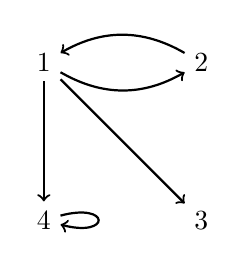
\begin{tikzpicture}
\node (atom1) at (0,2) {1};
\node (atom2) at (2,2) {2};
\node (atom3) at (2,0) {3};
\node (atom4) at (0,0) {4};
\draw[->, thick] (atom1) to[bend right] (atom2);
\draw[->, thick] (atom2) to[bend right] (atom1);
\draw[->, thick] (atom1)--(atom3);
\draw[->, thick] (atom1)--(atom4);
\draw[->, thick] (atom4) to[loop right, looseness=15] (atom4);
\end{tikzpicture}
\end{center}
The arrows represent the order in which `$R$' holds of the objects.  To indicate that 1 bears the relation represented by `$R$' to 4, we draw an arrow from 1 to 4, and to indicate that 4 bears the relation to itself, we draw an arrow that loops from 4 back to 4, and to indicate that 1 bears the relation to 2, and 2 also bears it to 1, we draw two arrows between them, and so on.  So there is one arrow for each pair in the extension of the predicate.

%Or we could give a diagram like this:
%\begin{center}
%\begin{tikzpicture}
%\node (atom1) at (0,2) {1};
%\node (atom2) at (2,2) {2};
%\node (atom3) at (2,0) {3};
%\node (atom4) at (0,0) {4};
%\draw[->, thick] (atom3)--(atom4);
%\draw[->, thick] (atom1) to[loop left, looseness=15] (atom1);
%\draw[->, thick] (atom3) to[loop right, looseness=15] (atom3);
%\draw[<->, thick] (atom1) -- (atom3);
%\end{tikzpicture}
%\end{center}
%to represent the following interpretation:
%	\begin{ekey}
%		\item[\text{Domain}] 1, 2, 3, 4
%		\item[R] \ntuple{1, 1}, \ntuple{1,3},  \ntuple{3, 1}, \ntuple{3, 3}, \ntuple{3,4}
%	\end{ekey}
%As you can probably guess, `$\forall xRxx$' would be false on both of our arrow diagrams, since neither diagram is one on which \emph{every} object bears the relation $R$ to itself.


If we wanted, we could make such arrow diagrams more complex. For example, we could label objects in our diagram with FOL names to indicate which object each name refers to.  To represent the extension of a one-place predicate in an arrow diagram, we could draw a circle around some objects and label the circle with the predicate. And to represent the extensions of multiple two-place predicates in a single arrow diagram, we might use arrows with dashed as opposed to solid lines, or arrows of different colors.



\section{Truth in FOL}\label{s:TruthFOL}

We have introduced interpretations. Our next task is to give a precise account of what it is for an arbitrarily complex FOL sentence to be true or false in a given interpretation. There are three kinds of sentence in FOL: atomic sentences, sentences whose main logical operator is a sentential connective, and lastly, sentences whose main logical operator is a quantifier.  We'll go through each kind in turn.

Our explanation will be completely general, but to make things comprehensible, it will be useful to have a particular interpretation to hand in order to give examples.  Let's use the following as our \emph{go-to interpretation}:
\begin{ekey}
		\item[\text{Domain}] all positive integers
		\item[a] 2
		\item[b] 3
		\item[E] \blank is even
		\item[R] \blank \ is less than \blank
	\end{ekey}
I've here specified the extensions of `$E$' and `$R$' indirectly, using English predicates, because I can't list all the numbers, or pairs of numbers, these are true of.  But the extension of `$E$' contains even numbers $2, 4, 6, 8 \ldots$, and the extension of `$R$' contains the pair \ntuple{2, 3}, as well as \ntuple{2, 4} and \ntuple{2,5} and \ntuple{3, 5}, and indeed every pair \ntuple{x,y} where $x$ is less than $y$.

\paragraph{Truth-Rule for Atomic Sentences} Determining the truth value of an atomic sentence on a given interpretation is fairly straightforward.  The atomic sentence `$Ea$', for example, is true just in case `$E$' is true of the referent of `$a$'.  Given our go-to interpretation, this sentence is true since `$a$' refers to 2, and 2 is indeed an even number.  By contrast, `$Eb$' would be false on our interpretation, because 3, which is the referent of `$b$', is not in the extension of `$E$', since it is not an even number.

Similarly, `$Rab$' is true on our interpretation just in case the referent of `$a$' is less than the referent of `$b$'.  Since 2 is indeed less than 3, `$Rab$' is true.  By contrast, `$Rba$' is not true, because 3 is not less than 2, or to put it another way, the pair \ntuple{3,2} is not in the extension of `$R$' on our interpretation.  Similarly, neither `$Raa$' nor `$Rbb$' are true on our go-to interpretation, since neither 2 nor 3 is less than itself (i.e. the pairs \ntuple{2,2} and \ntuple{3,3} are not in the extension of `$R$').  In general, the truth-rule for atomic sentences is:
	\factoidbox{
		When \meta{R} is an $n$-place predicate and $\meta{c}_1, \meta{c}_{2}, \ldots, \meta{c}_{n}$ are names, the sentence $\meta{R}\meta{c}_{1}\meta{c}_{2}\ldots\meta{c}_{n}$ is true in a given interpretation \textbf{iff} $\meta{R}$ is true of the objects referred to by $\meta{c}_{1}, \meta{c}_{2}, \ldots, \meta{c}_{n}$ (in that order) in that interpretation	}

%There is one additional kind of atomic sentence to consider: those formed by connecting two names with an identity sign.  As already mentioned, determining the truth values of identity statements is straightforward:
%\factoidbox{
%		For any names $\meta{a}$ and $\meta{b}$, the sentence $\meta{a} = \meta{b}$ is true in a given interpretation \textbf{iff}
%		 \meta{a} and \meta{b} refer to very same object in that interpretation
%	}
%So, in our go-to interpretation, `$a = b$' is false, since `$a$' refers to the number 2 and `$b$' to the number 3, and 2 is distinct from 3.  On the other hand, both `$a=a$' and `$b=b$' are true.

\paragraph{Truth-Rules for TFL Connectives} The truth rules governing our truth-functional operators are exactly the same as they were in TFL:

\factoidbox{
$\enot \meta{\varphi}$ is true in a given interpretation \textbf{iff} $\meta{\varphi}$ false in that interpretation\\

$(\meta{\varphi} \eand \meta{\psi})$ is true in a given interpretation \textbf{iff} both $\meta{\varphi}$ and $\meta{\psi}$ are true in that interpretation\\

$(\meta{\varphi} \eor \meta{\psi})$ is true in a given interpretation \textbf{iff} either $\meta{\varphi}$ or $\meta{\psi}$ is true in that interpretation\\


$(\meta{\varphi} \eif \meta{\psi})$ is true in a given interpretation \textbf{iff} either $\meta{\varphi}$ is false or $\meta{\psi}$ is true in that interpretation.\footnote{This means that $(\meta{\varphi} \eif \meta{\psi})$ is false if $\meta{\varphi}$ is true and  $\meta{\psi}$ is false, and true otherwise. }\\

$(\meta{\varphi} \eiff \meta{\psi})$ is true in a given interpretation \textbf{iff} $\meta{\varphi}$ has the same truth value as $\meta{\psi}$ in that interpretation
	}
This  is equivalent to the information conveyed by the characteristic truth tables for the connectives; it's just presented in words here rather than truth tables.   Some examples will help to illustrate the idea (make sure you understand them!). On our go-to interpretation:
	\begin{earg}
		\item[\textbullet]  `$\enot Raa$' is true because 2 is not less than itself
		\item[\textbullet] `$Rab \eand Ea$' is true because both conjuncts are true
		\item[\textbullet] `$Rab \eand Eb$' is false because, although `$Rab$' is true, `$Eb$' is false
		\item[\textbullet] `$Eb \eif \enot Rba$' is true because `$Eb$' is false.
		%\item[\textbullet] `$a=b \eor Ea$' is true because although `$a=b$' is false, `$Ea$' is true
		%\item[\textbullet] `$a \neq b \rightarrow Rba$' is false because the antecedent is true and the consequent is false
		\end{earg}

\section{Truth-Rules for Quantified Sentences}\label{s:TruthQuantifiedSentences}

The big innovation in FOL is the use of \emph{quantifiers}. And specifying the truth conditions for quantified sentences turns out to be a little tricky.  If we only look at simple cases things are pretty straightforward.  We can say that `$\exists xEx$' is true iff `$E$' is true of at least one object in the domain, and  `$\forall xEx$' is true iff `$E$' is true of every object in the domain.  So on our go-to interpretation, `$\exists xEx$' comes out true, and `$\forall xEx$' comes out false.


But what about a more complex sentence like `$\forall x(Ex \rightarrow Rxb)$'?  This has a universal quantifier as its main operator, so we might again try to say that it is true on an interpretation iff `$(Ex \rightarrow Rxb)$' is true of every object in the domain.  The trouble is that `$(Ex \rightarrow Rxb)$' is not a predicate, and our interpretation therefore does not directly specify what objects this complex formula is true of.  So while our simple-minded approach worked for `$\forall xEx$', it breaks down when we consider more complex sentences.  What we need is some \emph{uniform} and \emph{general} way of specifying the truth conditions of \emph{any} universally (or existentially) quantified sentence, irrespective of how complex it is.


The way we will do this is by temporarily treating variables like `$x$' \emph{as if} they referred to objects in the domain.  For example, we will say that the universal sentence `$\forall x(Ex \rightarrow Rxb)$' is true iff the formula `$(Ex \rightarrow Rxb)$' that the quantifier operates on is true \emph{no matter what object in the domain the variable `$x$'  is treated as referring to}. Of course, a variable like `$x$' doesn't actually refer to any particular thing, since it's not a name, and `$(Ex \rightarrow Rxb)$' doesn't actually have a truth value.  But if we temporarily treated `$x$' \emph{as if} it referred to 1, for example, then the conditional `$(Ex \rightarrow Rxb)$' would be true, since its antecedent `$Ex$' would be false (given that 1 is not even).


We will use the notion of a \define{variable assignment} to implement this idea of temporarily treating variables as if they refer to objects.  We can, for example, write $[x:1]$ for an assignment that treats `$x$' as referring to 1, and $[x:3]$ for an assignment that treats `$x$' as referring to 3.  So although the variable in `$Ex$' is not a name for any object in the domain, if we consider it \emph{relative to an assignment} like $[x:3]$, the variable works just like a name that refers to the number 3.  Such assignments can also cover multiple variables at once.  For example, $[x: 1, y:5, z:2]$ would be an assignment relative to which `$x$' refers 1, `$y$' refers to 5, and `$z$' refers to 2.  On our go-to interpretation, $(Ez \eand Rxy)$ would then be true relative to this assignment (since $2$ is even, and $1$ is less than $5$), but not relative to e.g. $[x:5, y: 2, z: 1]$.

Returning to `$\forall x(Ex \rightarrow Rxb)$', our idea is that to determine whether this is true, we go through each object in the domain, and ask whether `$(Ex \rightarrow Rxb)$' would come out true if `$x$' were treated as referring to that object.\footnote{Having brought assignments onto the scene, we should now technically go back and re-do our explanation of the truth conditions for atomic sentences too.  That's because we now need to determine the truth values of \emph{formulas} like `$(Ex \rightarrow Rxb)$' relative to an assignment of an object to the free variable `$x$', but our earlier explanation only covered \emph{sentences} (closed formulas), and said nothing about variable assignments.  See the Appendix for the technical details.}
So we have to ask ourselves:
\begin{enumerate}
\item[] is `$(Ex \rightarrow Rxb)$' true on $[x:1]$?
\item[] is `$(Ex \rightarrow Rxb)$' true on $[x:2]$?
\item[] is `$(Ex \rightarrow Rxb)$' true on $[x:3]$?
\item[] is `$(Ex \rightarrow Rxb)$' true on $[x:4]$?\\
$\vdots$
\end{enumerate}
and so on for every positive integer we could assign to `$x$'.  Now `$(Ex \rightarrow Rxb)$' is true on $[x:1]$ as well as $[x:3]$, since in both cases the antecedent `$Ex$' comes out false (because neither 1 nor 3 are even). And `$(Ex \rightarrow Rxb)$' is also true on $[x:2]$, since both `$Ex$' and `$Rxb$' are true on $[x:2]$ (because 2 is even, and also less than 3, which is what `$b$' refers to on our go-to interpretation).  An object that makes a formula like `$(Ex \rightarrow Rxb)$' true is said to \define{satisfy} that formula.  So the numbers 1, 2, and 3 all \emph{satisfy} `$(Ex \rightarrow Rxb)$'.

But the number 4 does \emph{not} satisfy it: `$(Ex \rightarrow Rxb)$' is \emph{false} on the assignment $[x:4]$.  That's because although `$Ex$' is true on $[x:4]$ (since 4 is even), `$Rxb$' is not true on $[x:4]$ (since 4 is \emph{not} less than 3).  So  since we found a number that makes`$(Ex \rightarrow Rxb)$' false, we can conclude that the universal sentence `$\forall x(Ex \rightarrow Rxb)$' we started with is itself false --- it isn't true of \emph{every} number.  And that's of course the result we want: relative to our go-to interpretation, `$\forall x(Ex \rightarrow Rxb)$' says that \emph{every} even number is less than three, which is clearly false, since there are lots of even numbers, including 4, that are not less than 3.

In practice, keeping track of variable assignments while calculating the truth value of a formula can get messy, especially when we're dealing with more than one variable.  We'll therefore make use a notational shorthand that will make things a little easier.  Instead of explicitly mentioning the variable assignment, we will use superscripts on the variables themselves to indicate what objects we are temporarily treating them as referring to.  So instead of saying:
$$`(Ex \rightarrow Rxb) \text{' is true on } [x:2]$$
as we did above, we will just add a superscript of $2$ to the variable `$x$' itself and write:
$$(Ex^2 \rightarrow Rx^2b) \text{ is true }$$
to indicate that we're treating $x$ as referring to 2.  Similarly, instead of saying that `$(Ez \eand Rxy)$' is true on $[x: 1, y:5, z:2]$, we can just say that $(Ez^2 \eand Rx^1y^5)$ is true.

You can think of $(Ex^2 \rightarrow Rx^2b)$ as a \define{semantic instance} of $\forall x(Ex \rightarrow Rxb)$, much like $(Ea \rightarrow Rab)$ is a \emph{syntactic instance} of $\forall x(Ex \rightarrow Rxb)$, something we could infer by $\forall E$.  In both cases, we delete the quantifier, and then do something with the variable the quantifier bound: in the case of syntactic instances, we replace the variable with a name, and in the case of semantic instances, we assign an object from the domain to the variable.  
\factoidbox{Given a quantified FOL sentence $\forall \meta{v}\meta{\varphi}(\ldots \meta{v} \ldots)$ or $\exists \meta{v}\meta{\varphi}(\ldots \meta{v} \ldots)$, its \define{semantic instances} in an interpretation  \script{I} are obtained by removing the quantifier and assigning some object $o$ from  \script{I}'s domain to every occurrence of the variable $\meta{v}$ bound by that quantifier $\meta{\varphi}(\ldots \meta{v}^o \ldots)$.}
It's important to remember, though, that this really is just a notational shorthand.  Whereas the syntactic instance $(Ea \rightarrow Rab)$ is a genuine sentence of FOL, the semantic instance $(Ex^2 \rightarrow Rx^2b)$ is not a sentence of FOL (nor even a formula), since the language of FOL doesn't include superscripts on variables.  Talk of $(Ex^2 \rightarrow Rx^2b)$ is, again, just shorthand for talking about the FOL formula `$(Ex \rightarrow Rxb)$' relative to an assignment of 2 to `$x$'.

With this background in place, we can now state the truth-rules for quantified sentencess:
\factoidbox{$\forall \meta{v}\meta{\varphi}(\ldots \meta{v} \ldots)$ is true in an interpretation \script{I} \textbf{iff}  $\meta{\varphi}(\ldots \meta{v}^o \ldots)$ is true in \script{I} for \emph{every object} $o$ in \script{I}'s domain (i.e. if \emph{all} of its semantic instances in \script{I} are true).\\

$\exists \meta{v}\meta{\varphi}(\ldots \meta{v} \ldots)$ is true in an interpretation \script{I} \textbf{iff}  $\meta{\varphi}(\ldots \meta{v}^o \ldots)$ is true in \script{I} for \emph{at least one} object $o$ in \script{I}'s domain (i.e. if \emph{at least one} of its semantic instances in \script{I} are true).
}
The idea, again, is that we go through each object $o$ in the domain, and check whether $\meta{\varphi}(\ldots \meta{v} \ldots)$ is true if \meta{v} is treated as referring to $o$; if so, the universal sentence $\forall \meta{v}\meta{\varphi}(\ldots \meta{v} \ldots)$ is true, if not, it's false.  Notice that it's much easier for an existential sentence to be true: for $\exists \meta{v}\meta{\varphi}(\ldots \meta{v} \ldots)$ to be true, it suffices if \emph{one} object in the domain satisfies $\meta{\varphi}(\ldots \meta{v} \ldots)$.


This in turn means that that it's very easy for a universal sentence $\forall \meta{v}\meta{\varphi}(\ldots \meta{v} \ldots)$ to be \emph{false}: we just have to find a single object that makes $\meta{\varphi}(\ldots \meta{v} \ldots)$ false.  For an existential sentence $\exists \meta{v}\meta{\varphi}(\ldots \meta{v} \ldots)$ to be false, on the other hand, we have to make sure that $\meta{\varphi}(\ldots \meta{v} \ldots)$ is false for \emph{every} object in the domain. Let's state these ``falsity conditions'' too:
\factoidbox{$\forall \meta{v}\meta{\varphi}(\ldots \meta{v} \ldots)$ is false in a given interpretation \script{I} \textbf{iff}  $\meta{\varphi}(\ldots \meta{v}^o \ldots)$ is false in \script{I} for \emph{at least one object} $o$ in \script{I}'s domain.\\

$\exists \meta{v}\meta{\varphi}(\ldots \meta{v} \ldots)$ is false in a given interpretation \script{I} \textbf{iff}  $\meta{\varphi}(\ldots \meta{v}^o \ldots)$ is false in \script{I} for \emph{every} object $o$ in \script{I}'s domain.
}
Again, we're here suppressing explicit mention of variable assignments via our notational shorthand, but you can look at the Appendix for the official version of the semantics, with variable assignments made explicit.  Let's now go through a few examples to get a better feel for how to determine the truth values of quantified sentences.






\section{Truth in an Interpretation: Examples}

 Since the number of objects we have to consider increases the larger the domain is, we'll here use interpretations with relatively small domains.  Let's start with the following interpretation with just three objects in its domain:\\

\begin{minipage}{\textwidth}
\begin{center}
\textbf{Interpretation A}
\begin{multicols}{2}
	\begin{ekey}
		\item[\text{Domain}] 1, 2, 3
		\item[F] 1
		\item[G] 2, 3
		\item[H]
	\end{ekey}
\columnbreak

\begin{center}\begin{tabular}{|c|c|c|c|}
\hline
    &   F   &   G  & H  \\ \hline
1   &   $+$   &   $-$  & $-$  \\ \hline
2   &   $-$   &   $+$ & $-$ \\ \hline
3   &   $-$   &   $+$ & $-$ \\ \hline
\end{tabular}\end{center}
\end{multicols}
\end{center}
\end{minipage}


\paragraph{Example 1} $\exists x(Fx \eand Gx)$

\noindent For this to be true, it suffices if a single object in the domain satisfies `$(Fx \land Gx)$'.  Unfortunately, no matter which object we treat `$x$' as referring to, it comes out false.  So our original existential sentence is false.  Our explanation in other words goes like this:

\begin{etriangle}
\item $\exists x(Fx \eand Gx)$ is false because `$(Fx \eand Gx)$' is false for every object in the domain:
\begin{etriangle}
\item $(Fx^1 \eand Gx^1)$ is false (since $Gx^1$ is false), and
\item $(Fx^2 \eand Gx^2)$ is also false (since $Fx^2$ is false), and
\item $(Fx^3 \eand Gx^3)$ is also false (since $Fx^3$ is false)
\end{etriangle}
\end{etriangle}
%Again, when in the course of this explanation I say that $(Fx^3 \eand Gx^3)$ is false,  for example, this is just a shorthand for saying that `$(Fx \eand Gx)$' is false if `$x$' is temporarily treated as referring to the number 3.

\paragraph{Example 2} $\exists x Fx \land \exists x Gx$

\noindent Notice that the main operator in this is $\eand$, i.e. it's a conjunction.  So here we \emph{first} have to apply the truth-rule for $\land$, and evaluate its two conjuncts $\exists xFx$ and $\exists xGx$ \emph{separately}.  And to determine the truth value of each conjunct, we then use the truth-rule for existential sentences.    As it turns out, both $\exists xFx$ and $\exists xGx$ are true, meaning that our conjunction as a whole also comes out true:
\begin{etriangle}
\item $\exists x Fx \land \exists x Gx$ is true, because
\begin{etriangle}
\item $\exists xFx$ is true
\begin{etriangle}
\item that's because $Fx^1$ is true
\end{etriangle}
\item and $\exists xGx$ is also true
 \begin{etriangle}
 \item that's because $Gx^2$ is true
\end{etriangle}
\end{etriangle}
\end{etriangle}
Notice that $Gx^3$ is of course also true, so I could instead have given this as my reason for why $\exists xGx$  is true.   It doesn't matter whether I pick 2 or 3 --- as long as I can point to at least one object that satisfies `$Gx$', that's enough for $\exists xGx$ to be true.

What these two examples illustrate is that we always have to identify the main operator, and then apply the truth-rule appropriate to that operator.  In `$\exists x(Fx \eand Gx)$', the main operator is the existential quantifier, so I apply the truth-rule for the quantifier, and see whether I can find an object to make the whole conjunction `$(Fx \eand Gx)$' true.  In `$\exists x Fx \land \exists x Gx$', by contrast, the main operator is $\land$, so here I do not have to find a single object to make both `$Fx$' and `$Gx$' true.  Rather I consider the two conjucts `$\exists x Fx$' and `$\exists x Gx$' \emph{separately}. Then I check, first, whether any object satisfies `$Fx$', and second whether any object (perhaps a different one) satisfies `$Gx$'.  Since I can find an object in each case, both `$\exists x Fx$' and `$\exists x Gx$' are true; and this means that `$\exists x Fx \land \exists x Gx$' is true by the truth-rule for conjunction.

Things get  more complicated with sentences that contain nested quantifiers, like $\exists x\forall yLxy$.  Let's determine the truth value of this on the following interpretation:\\

\begin{minipage}{\textwidth}
\begin{center}
\textbf{Interpretation B}
\begin{multicols}{2}
	\begin{ekey}
		\item[\text{Domain}] 1, 2, 3
		\item[L] \ntuple{2,1}, \ntuple{2,2}, \ntuple{2, 3}
	\end{ekey}
\columnbreak

\begin{tikzpicture}
\node (atom1) at (0,2) {1};
\node (atom2) at (2,2) {2};
\node (atom3) at (2,0) {3};
\draw[->, thick] (atom2)--(atom1);
\draw[->, thick] (atom2)--(atom3);
\draw[->, thick] (atom2) to[loop right, looseness=15] (atom2);
%\draw[->, thick] (atom4) to[loop right, looseness=15] (atom4);
\end{tikzpicture}
\end{multicols}
\end{center}
\end{minipage}

\paragraph{Example 3} $\exists x\forall yLxy$

\noindent If we paraphrase this in English, it says that there is some object $x$ which bears the relation $L$ to \emph{every} object y.  And indeed there is such an object in  Interpretation B, namely the number 2: this number bears $L$ to 1, and to itself, and also to 3, that is, to every object in the domain.

To put the same point formally: in   order for `$\exists x\forall yLxy$' to be true, there has to be at least one object $o$ that makes $\forall yLx^oy$ true.  And there is such an object, namely 2.  So `$\exists x\forall yLxy$' is true because $\forall yLx^2y$  is true.  Next we ask why $\forall yLx^2y$ is true.  That's because no matter which object $o$ we pick for $y$ to refer to, `$Lx^2y^o$' comes out true.  That is, $Lx^2y^1$, and $Lx^2y^2$ and $Lx^2y^3$ are all true. Our official explanation in other words looks like this:

\begin{etriangle}
\item $\exists x\forall yLxy$ is true because:
\begin{etriangle}
\item $\forall yLx^2y$ is true.  And this is because:
\begin{etriangle}
\item $Lx^2y^1$ is true, and
\item $Lx^2y^2$ is true, and
\item $Lx^2y^3$ is true
\end{etriangle}
\end{etriangle}
\end{etriangle}

Although sentences with nested quantifiers occur most commonly with many-place predicates, nested quantifiers can occur in combination with just one-place predicates too.  Let's return to Interpretation A, and consider a case like this for our final example.

\paragraph{Example 4} $\exists x(Fx \eif \forall y(Hy \eiff Gx))$

\noindent The main operator is the existential quantifier, so its truth-rule tells us that we have to see whether there is any object $o$ that would make $(Fx^o \eif \forall y(Hy \eiff Gx^o))$ true on Interpretation A.  In fact, an assignment of 1 to `$x$' will do it: the conditional $(Fx^1 \eif \forall y(Hy \eiff Gx^1))$ comes out true because its antecedent $Fx^1$ is true and its consequent $\forall y(Hy \eiff Gx^1)$ is also true.


To explain why `$\forall y(Hy \eiff Gx^1)$'  is true, we need to apply the truth-rule for the universal quantifier: this is true is because no matter what object $o$  we pick, $Hy^o \eiff Gx^1$ is true.  That is:  $Hy^1 \eiff Gx^1$ is true, and $Hy^2 \eiff Gx^1$ is true, and $Hy^3 \eiff Gx^1$ is  also true. The complete explanation for why Example 4 is true on Interpretation A then looks like this:


\begin{etriangle}
\item $\exists x(Fx \eif \forall y(Hy \eiff Gx))$ is true because:
\begin{etriangle}
\item $Fx^1 \eif \forall y(Hy \eiff Gx^1)$ is true.  And this is because:
\begin{etriangle}
\item $Fx^1$ is true, and
\item $\forall y(Hy \eiff Gx^1)$ is also true. This in turn is because:
\begin{etriangle}
\item $(Hy^1 \eiff Gx^1)$ is true (since $Hy^1$ and $Gx^1$ are both false) and
\item $(Hy^2 \eiff Gx^1)$ is true (since $Hy^2$ and $Gx^1$ are both false) and
\item $(Hy^3 \eiff Gx^1)$ is true (since $Hy^3$ and $Gx^1$ are both false)
\end{etriangle}
\end{etriangle}
\end{etriangle}
\end{etriangle}


An explanation of this sort is called a \define{semantic demonstration} of the truth or falsity of a given sentence (in an interpretation).  In the exercises below, you should give semantic demonstrations like this to justify your claims about the truth values of sentences.



\practiceproblems

\problempart Take the following interpretation, and determine the truth value of each sentence below on this interpretation (remember to give a semantic demonstration in each case):\\

\begin{minipage}{\textwidth}
\begin{multicols}{2}
	\begin{ekey}
		\item[\text{Domain}] 1, 2
		\item[F] 1, 2
		\item[G] 2
		\item[H]
	\end{ekey}
	
\columnbreak

\begin{tabular}{|c|c|c|c|}
\hline
    &   F   &   G  & H  \\ \hline
1   &   $+$   &   $-$  & $-$  \\ \hline
2   &   $+$   &   $+$ & $-$ \\ \hline
\end{tabular}

\end{multicols}
\end{minipage}



\begin{earg}
\item $\exists x(Fx \eand Gx)$
\item $\forall x(Hx \eif Gx)$
\item $\forall x(Fx \eif \enot Hx)$
\item $\forall x(Fx \eiff Gx)$
\item $\forall xGx \eif \exists y Hy$
\item $\forall xFx \eand \enot \exists xGx$
\item $\exists x(Gx \land \forall y(Gy \eif Hx))$
\item $\forall x(Gx \eif \exists y(Fx \eand \enot Gy))$ % NOTE: make this one false in future
\end{earg}


%\problempart
%\label{pr.TorF1}
%Consider the following interpretation:\footnote{See \S\ref{s:FOLInterpretations} on how diagrams like the one to the right are used to represent interpretations. In a matrix diagram like this, a lower-case letter to the left of a domain-object indicates that it is a name of that object. }
%
%
%\begin{multicols}{2}
%\begin{ekey}
%		\item[\text{Domain}] 1, 2
%		\item[a] 1
%		\item[A] 1, 2
%		\item[B] 2
%		\item[N]
%\end{ekey}
%\columnbreak
%
%\begin{tabular}{c|c|c|c|c|}
%\hline
%&    &   A   &   B  & N  \\ \hline
%a & 1 &   $+$   &   $-$  & $-$  \\ \hline
% & 2   &   $+$   &   $+$ & $-$ \\ \hline
%\end{tabular}
%\end{multicols}
%
%
%\noindent Determine whether each of the following sentences is true or false in this interpretation, and give a semantic demonstration to justify your answer.
%\begin{earg}
%\item $Ba$
%\item $Aa \eiff \enot Na$
%\item $Na \eif (Aa \eor Ba)$
%\item $\forall x Ax$
%\item $\forall x \enot Bx$
%\item $\exists x(Ax \eand Bx)$
%\item $\exists x(Ax \eif Nx)$
%\item $\forall x(Nx \eor \enot Nx)$
%\item $\exists x Bx \eif \forall x Ax$
%\end{earg}

%\problempart
%Consider the following interpretation:
%
%
%\begin{multicols}{2}
%\begin{ekey}
%		\item[\text{Domain}] 1, 2, 3
%		\item[b] 2
%		\item[c] 3
%		\item[G] 1, 2, 3
%		\item[H] 2
%		\item[M] 1, 3
%\end{ekey}
%\columnbreak
%
%\begin{tabular}{c|c|c|c|c|}
%\hline
%&    &   G  &   H  & M  \\ \hline
% & 1 &   $+$   &   $-$  & $+$  \\ \hline
%b & 2   &   $+$   &   $+$ & $-$ \\ \hline
%c  & 3   &   $+$   &   $-$ & $+$ \\ \hline
%\end{tabular}
%\end{multicols}
%
%
%
%\noindent Determine whether each of the following sentences is true or false in this interpretation, and give a semantic demonstration to justify your answer.
%\begin{earg}
%\item $Hc$
%\item $Hb$
%\item $Mc \eor Mb$
%\item $Gc \eor \enot Gc$
%\item $Mc \eif Gc$
%\item $\exists x Hx$
%\item $\forall x Hx$
%\item $\exists x \enot Mx$
%\item $\exists x(Hx \eand Gx)$
%\item $\exists x(Mx \eand Gx)$
%\item $\forall x(Hx \eor Mx)$
%\item $\exists x Hx \eand \exists x Mx$
%\item $\forall x(Hx \eiff \enot Mx)$
%\item $\exists x Gx \eand \exists x \enot Gx$
%\item $\forall x\exists y(Gx \eand Hy)$
%\end{earg}

\problempart
\label{pr.TorF3} Determine the truth values of the sentences below on the provided interpretation
%\begin{center}
%\begin{tikzpicture}
%\node (atom1) at (0,2) {1};
%\node (atom2) at (2,2) {2};
%\node (atom4) at (0,0) {3};
%\node (atom5) at (2,0) {4};
%\node (atom6) at (4,0) {5};
%\draw[->, thick] (atom1)+(-0.15,0.15) arc (-330:-30:.3);
%\draw[->, thick] (atom6)+(0.15,-0.15) arc (-150:150:.3);
%\draw[->, thick] (atom1) -- (atom2);
%\draw[->, thick] (atom1) -- (atom4);
%\draw[<->, thick] (atom1) -- (atom5);
%\draw[->, thick] (atom1) -- (atom6);
%\draw[->, thick] (atom2) -- (atom6);
%\end{tikzpicture}
%\end{center}


\begin{multicols}{2}
	\begin{ekey}
		\item[\text{Domain}] 1, 2, 3
		\item[R] \ntuple{1,3}, \ntuple{2,2}, \ntuple{2,3}, \ntuple{3, 2} \ntuple{3,3}
	\end{ekey}
\columnbreak

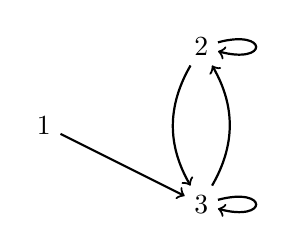
\begin{tikzpicture}
\node (atom1) at (0,1) {1};
\node (atom2) at (2,2) {2};
\node (atom3) at (2,0) {3};
\draw[->, thick] (atom1)--(atom3);
\draw[->, thick] (atom2) to[bend right] (atom3);
\draw[->, thick] (atom3) to[bend right] (atom2);
\draw[->, thick] (atom3) to[loop right, looseness=15] (atom3);
\draw[->, thick] (atom2) to[loop right, looseness=15] (atom2);
%\draw[->, thick] (atom4) to[loop right, looseness=15] (atom4);
\end{tikzpicture}

\end{multicols}



\begin{earg}
\item $\exists x Rxx$
\item $\forall x Rxx$
\item $\forall x \forall yRxy$
\item $\forall x\exists yRxy$
\item $\exists x \forall y Rxy$
%\item $\exists x \forall y Ryx$
\item $\exists x \forall y \enot Ryx$
\item $\forall y \exists x\enot Ryx$
\item $\forall x \forall y(Rxy \rightarrow Ryx)$
\item $\exists x\forall y(Rxy \rightarrow Ryx)$
\item $\forall x(\exists y Rxy \eif \exists y Ryx)$
%\item $\exists x \exists y (\enot x = y \eand Rxy \eand Ryx)$
%\item $\exists x \forall y(Rxy \eiff x = y)$
%\item $\exists x \forall y(Ryx \eiff x = y)$
%\item $\forall x \forall y \forall z ((Rxy \eand Ryz) \eif Rxz)$
%\item $\exists x \forall y \forall z ((Rxy \eand Ryz) \eif Rxz)$
%\item $\exists x \exists y(\enot x = y \eand Rxy \eand \forall z(Rzx \eiff y = z))$
\end{earg}

\problempart Determine the truth values of the sentences below on the provided interpretation (note that in the diagram, I am using an oval to indicate the extension of the 1-place predicate `$F$', and arrows for the extension of the 2-place predicate `$R$'):\\


\begin{minipage}{\textwidth}
\begin{multicols}{2}

	\begin{ekey}
		\item[\text{Domain}] 1, 2, 3
		\item[F] 1
		\item[R] \ntuple{1,1}, \ntuple{1,2}, \ntuple{1,3}, \ntuple{2,3}  \ntuple{3,2}, \ntuple{3,3}
		
	\end{ekey}

\columnbreak
	
\begin{tikzpicture}[>=stealth',thick]

\node (1) {1};
\node (2) [right=of 1] {2};
\node (3) [right=of 2] {3};



\draw (0,0) circle [x radius=0.6cm, y radius =1.2cm] node [left =0.5cm] {$F$};


\path (1) edge[->] (2);
\path (2) edge[->] (3);
\path (3) edge[->, bend right] (2);
\path (3) edge[->,loop above] (3);
\path (1) edge[->,bend right] (3);
\path (1) edge[->,loop above] (1);

\end{tikzpicture}
\end{multicols}
\end{minipage}




\begin{earg}

\item $\exists x(Fx \eand Rxx)$
\item $\exists x(\enot Fx \eand \enot Rxx)$
\item $\forall x(Rxx \rightarrow Fx)$
\item $\forall x(\exists yRxy \eif Fx)$
\item $\forall x\exists y Rxy$
\item $\forall x\exists yRxy \eif \exists xFx$
\item $\exists x(\forall y Rxy \eand \exists yRyx)$

\end{earg}




\section{Semantic Concepts}\label{s:FOLSemanticConcepts}

Defining truth in FOL was a bit tricky, due to the presence of quantifiers. But now that we know what determines the truth value of an FOL sentence in an interpretation, we can use that to define various other central logical notions.   As you can see, these definitions are basically the same as those from TFL, except that we here use the notion of truth in an \emph{interpretation} rather than truth on a \emph{valuation}.  In all the definitions below, the metavariables $\meta{\varphi}_1 \ldots \meta{\varphi}_n$ and $\meta{\psi}$ range over arbitrary \emph{sentences} of FOL:\footnote{Our logical concepts are in other words only defined for FOL sentences.  By contrast, the official explanation of truth in FOL, given in the Appendix, covers formulas in general, not just sentences.}

\factoidbox{
	$\meta{\varphi}_1, \ldots, \meta{\varphi}_n$ \define{logically entail}  $\meta{\psi}$, written $\meta{\varphi}_1, \ldots, \meta{\varphi}_n \vDash \meta{\psi}$,   iff no interpretation makes all of $\meta{\varphi}_1,  \ldots, \meta{\varphi}_n$ true but $\meta{\psi}$ false.\\

\meta{\varphi} is a \define{Logical Truth}, written $\vDash \meta{\varphi}$, iff it is true in every interpretation.\\

\meta{\varphi} is a \define{contradiction}  iff it is false in every interpretation.\\

\meta{\varphi} and \meta{\psi} are \define{logically equivalent}, written $\meta{\varphi} \lequiv \meta{\psi}$ iff they have the same truth value in every interpretation.\\

$\meta{\varphi}_1,\ldots, \meta{\varphi}_n$ are \define{jointly consistent} iff there is at least one interpretation which makes them all true.  They are \define{jointly inconsistent} iff there is no such interpretation.
}

As in TFL, perhaps the most important of these concepts is  entailment, since it is closely related to the notion of a valid argument.  We will say that an FOL argument:
$$\meta{\varphi}_1, \ldots, \meta{\varphi}_n \therefore \meta{\psi}$$
is \define{valid} just in case its premises $\meta{\varphi}_1, \ldots, \meta{\varphi}_n$ logically entail its conclusion \meta{\psi}.  Since entailment is defined in terms of the concept of truth-in-an-interpretation, we can use interpretations to investigate the validity of FOL arguments.

In particular, we can use interpretations to show that an argument is \emph{not} valid, or that the corresponding entailment \emph{fails}.  To show that a given argument is not valid, it suffices to construct a single interpretation that simultaneously makes all of the premises true but still makes the conclusion false.  Such an interpretation is again called a \emph{counterexample} to the validity of the argument, or a \define{countermodel}.


In the next two sections, we'll look at how to construct countermodels.  We'll first look at arguments that involve only one-place predicates, and then at ones that involve many-place predicates.  Of course, we can use interpretations to investigate the other logical concepts we've defined above too.  We'll return to that once we've looked at our central concept of entailment, or validity.

\section{Countermodels with One-Place Predicates}\label{s:CountermodelOnePl}

\paragraph{Example 1} Let's begin with one of the examples we looked at way back in \S\ref{s:Arguments}.

\begin{earg}
\item[\ex{exarg4}]All rabbits are mammals
\item[] Bugs Bunny is a mammal.
\item[] $\therefore$ Bugs Bunny is a rabbit.
\end{earg}

\noindent As we noted at the time, this argument is intuitively not valid.  We are now in a position to demonstrate this formally.  First, we can offer the following FOL symbolization:
\begin{earg}
\item[] $\forall x(Rx \eif Mx)$
\item[] $Mb$
\item[] $\therefore$ $Rb$
\end{earg}
\noindent Next, we can construct an interpretation which makes the premises true and the conclusion false.  One such interpretation would be the following:
\begin{ekey}
	\item[\text{Domain}] all people
	\item[b] Lady Gaga
	\item[R] \blank \ is an opera singer
	\item[M] \blank\ is a vocalist
\end{ekey}
In this interpretation, `$\forall x(Rx \eif Mx)$' is  true, since every opera singer is a vocalist, and `$Mb$' is also true, since Lady Gaga is a vocalist.  But `$Rb$' is false, since she is not an opera singer, but a pop singer.  So the argument isn't valid.  However, using this kind of countermodel  has the drawback that it requires us to appeal to real-world knowledge.   After all, who knows, maybe, Lady Gaga secretly performs in operas too, in which case `$Rb$' is true in this interpretation, and it doesn't constitute a countermodel after all.

To avoid these kinds of issues, and to give some uniformity to our countermodels, we will again use interpretations with domains that contain just positive integers, and give \emph{direct} specifications of the extensions of predicates, by listing the objects they are true of.  Furthermore, since we may have to explain why universal sentences like `$\forall x(Rx \eif Mx)$' are true on our countermodels, and since the number of objects we have to consider to do this increases the larger the domain is, we will  try to construct countermodels  with the smallest possible domains.

Let's begin by seeing if we can construct a countermodel that has just one object in its domain, say the number 1.  First off, let's make sure our conclusion `$Rb$' is false.  To that end, we can let `$b$' refer to 1, and let the extension of the predicate `$R$' remain empty.  And to make the second premise, `$Mb$' true, we have to put 1 (the referent of `$b$') into the extension of `$M$'.  So we have an interpretation like this:

\begin{center}
\begin{minipage}{0.7\textwidth}
\begin{multicols}{2}
\begin{ekey}
	\item[\text{Domain}] 1
	\item[b] 1
	\item[R]
	\item[M] 1
\end{ekey}
\columnbreak
\begin{tabular}{c|c|c|c|}
\hline
 & &   R  & M  \\ \hline
b& 1   &   $-$  & $+$  \\ \hline
\end{tabular}
\end{multicols}\end{minipage}\end{center}
And luckily this also makes the first premise `$\forall x(Rx \eif Mx)$' true!  After all, $(Rx^1 \eif Mx^1)$ is true (since $Rx^1$ is false).  And since 1 is the only object in our domain, that suffices for `$\forall x(Rx \eif Mx)$'  to be true!  So our simple interpretation makes both premises true but the conclusion false, showing that the argument isn't valid.

\paragraph{Example 2} Let's look at a slightly more complex example:
$$\exists x(Fx \eif Gx) \therefore \exists xFx \eif \exists xGx$$
We will again begin with the smallest possible domain, containing just 1, and think about what's needed to make the conclusion, `$\exists xFx \eif \exists xGx$' false.  Since this is a conditional, we have to make its antecedent `$\exists x Fx$' true and its consequent `$\exists xGx$' false.  Using just the number 1, we can do that as follows:
\begin{center}\begin{tabular}{|c|c|c|}
\hline
&   F  & G  \\ \hline
1   &   $+$  & $-$  \\ \hline
\end{tabular}\end{center}
`$\exists xFx$' is now true, since $Fx^1$ is true.  But `$\exists xGx$' is false, because $Gx^1$ is false. The trouble is that this interpretation will also make our premise `$\exists x(Fx \eif Gx)$' false.  After all, $(Fx^1 \eif Gx^1)$ is false, and there's no other object in the domain we could assign to `$x$' to make `$(Fx \eif Gx)$' true.

So let's expand our domain by adding a second object:
\begin{center}\begin{tabular}{|c|c|c|}
\hline
&   F  & G  \\ \hline
1   &   $+$  & $-$  \\ \hline
2 &     ?    &  ?    \\ \hline
\end{tabular}\end{center}
We don't yet know whether our two predicates should be true or false of this new object, so I've left the cells next to it blank.  Let's begin with our conclusion `$\exists xFx \eif \exists xGx$' again: we want it to be false, so `$\exists xFx$' has to be true and `$\exists xGx$' has to be false.  Of course, `$\exists xFx$' remains true because $Fx^1$ is still true, so no change is needed here.  But to keep `$\exists xGx$' false, we need to make sure that our new object 2 is not in the extension of `$G$' either:
\begin{center}\begin{tabular}{|c|c|c|}
\hline
&   F  & G  \\ \hline
1   &   $+$  & $-$  \\ \hline
2 &     ?    &   $-$   \\ \hline
\end{tabular}\end{center}
Now, can we make the premise `$\exists x(Fx \eif Gx)$' true?  In fact we can, by making sure that `$F$' is not true of 2.  For in that case, $(Fx^2 \eif Gx^2)$ will be true, because the antecedent $Fx^2$ will be false.  And that suffices for the truth of `$\exists x(Fx \eif Gx)$'.  Our final countermodel, and the accompanying semantic demonstrations showing that our premise is true and our conclusion false, then look like this:

\begin{center}
\begin{minipage}{0.7\textwidth}
\begin{multicols}{2}
\begin{ekey}
	\item[\text{Domain}] 1, 2
	\item[F] 1
	\item[G]
\end{ekey}
\columnbreak
\begin{tabular}{|c|c|c|}
\hline
&   F  & G  \\ \hline
1   &   $+$  & $-$  \\ \hline
2 &     $-$    &   $-$   \\ \hline
\end{tabular}
\end{multicols}\end{minipage}\end{center}



\begin{ebullet}
\item $\exists x(Fx \eif Gx)$ is true because:
\begin{etriangle}
\item $(Fx^2 \eif Gx^2)$ is true (since $Fx^2$ is false)
\end{etriangle}
\end{ebullet}

\begin{ebullet}
\item $\exists xFx \eif \exists x Gx$ is false because:
\begin{etriangle}
\item $\exists xFx$ is true
\begin{etriangle}
\item since $Fx^1$ is true
\end{etriangle}
\item but $\exists xGx$ is false.  This is because
\begin{etriangle}
\item $Gx^1$ is false, and
\item $Gx^2$ is also false
\end{etriangle}
\end{etriangle}
\end{ebullet}


We only needed a single object in the domain of our first countermodel, but our second countermodel ended up requiring two objects to simultaneously make the premises true and the conclusion false.  Other examples might require you to use three objects, or even four, or more.  Is there any upper bound on the number of objects that might be needed to produce a countermodel?

It turns out that for arguments that only involve one-place predicates, the answer is `yes'.  The logician Leopold L\"owenheim showed that if an FOL argument contains just $n$ one-place predicates, then if the argument is invalid, a countermodel with a domain of at most $2^n$ objects exists.  So for something like Example 2, which involves two one-place predicates, we can be sure that we won't need more than four objects.  As we'll see, there is no such upper bound for arguments with many-place predicates.


Before we turn to many-place predicates, though, one more general observation is in order.  Consider the following English argument:
\begin{earg}
	\item[] All foxes are mortal.
	\item[$\therefore$] Every vixen is mortal.
\end{earg}
This argument is valid in the sense that it's impossible for its premise to be true but its conclusion to be false: a vixen is just a female fox, so any possible world where every fox is mortal has to be one where every vixen is mortal.  But if we symbolize it, the resulting FOL argument is \emph{not} valid:
\begin{earg}
	\item[] $\forall x(Fx \eif Mx)$
	\item[$\therefore$] $\forall x(Vx \eif Mx)$
\end{earg}
It's easy to construct an interpretation that makes the premise true and the conclusion false (just put an object in the extension of $V$ but not $M$ or $F$).

So from the fact that the symbolization of an English argument in FOL is not valid, we can't straightaway conclude that the original English argument is not valid.   What we can conclude is just that the original English argument is not \emph{formally} valid, or more specifically, that it isn't valid in virtue of the kind of logical form captured in its FOL symbolization.  But it might still be valid for other reasons --- in this case, because of the connection between the meanings of `fox' and `vixen'.  As we discussed in \S\ref{s:FormalValidity}, logic doesn't aim to capture the validity of arguments like this; it only cares about formally valid arguments.\footnote{Of course we can make the above argument formally valid by adding a second premise: `Every vixen is a fox', which we'd symbolize as `$\forall x(Vx \eif Fx)$'.  But this is now a \emph{different}  $FOL$ argument, one with two premises.}

\practiceproblems
\problempart Construct countermodels to demonstrate the following:

\begin{earg}
\item $\forall xFx \eiff \forall x Gx \nvDash \forall x(Fx \eiff Gx)$ % Needs 1
\item $\forall x ((Fx \eand Gx) \eif Hx) \nvDash \forall x(Fx \eor Gx) \eor \forall x(Fx \eor Hx)$ %Needs 1
\item $\forall xFx \eif \exists xGx \nvDash \exists x Fx \eif \exists x Gx$ % Needs 2
\item $(\forall x Fx \eand \forall x Gx) \eif \forall x Hx \nvDash \forall x((Fx \eand Gx) \eif Hx)$ % Needs 2
\item $\exists x\forall y(Fx \eif Gy) \nvDash \exists y\forall x(Fx \eif Gy)$
\item $\forall x \exists y(Fy \eif Gx) \nvDash \forall x(\exists yFy \eif Gx)$ % Needs 2
\item $\forall x(\exists yFy \eif Gx) \nvDash \forall x \exists y(Fy \eif Gx)$
\end{earg}



\section{Countermodels with Many-Place Predicates}

Let's next look at how to construct countermodels for arguments with many-place predicates.  First, though, there's some new terminology that will come in handy.  Two-place predicates like `loves', `respects', `admires' etc. express \define{relations} between objects (the loving relation, the respecting relation, and so on).  And there are some important characteristics that relations like this can have:

\factoidbox{
A relation $R$ is \define{serial} iff $\forall x \exists y Rxy$

A relation $R$ is \define{reflexive} iff $\forall xRxx$

A relation $R$ is \define{symmetric} iff $\forall x \forall y(Rxy \eif Ryx)$

A relation $R$ is \define{transitive} iff $\forall x \forall y \forall z((Rxy \eand Ryz) \eif Rxz)$
}
One thing we can do, then, is to show that a relation's having certain of these characteristics does, or does not, imply its having some other characteristic.  For example, being reflexive implies being serial. After all: if every object bears $R$ to itself, then every object bears $R$ to \emph{at least} one thing, namely itself!  You could do a natural deduction proof to show that $\forall x Rxx \vdash \forall x \exists y Rxy$.  However, the implication does not hold in the other direction, i.e. being serial does \emph{not} imply being reflexive.  Showing this will be our first example.

\paragraph{Example 1} $\forall x \exists y Rxy \nvDash \forall xRxx$

You can perhaps already think of a countermodel that would make `$\forall x \exists y Rxy$' true but `$ \forall xRxx$' false, but again, we're going to try to find the smallest countermodel to do the job.  Let's start with a domain that just contains the number 1.  For `$\forall x \exists y Rxy$' to be true, every object in the domain has to bear the relation $R$ to at least one object.  So since we only have one object, that means 1 has to bear $R$ to itself:
\begin{center}
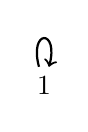
\begin{tikzpicture}
\node (atom1) {1};
\draw[->, thick] (atom1) to[loop above] (atom1);
\end{tikzpicture}
\end{center}
However, this now also makes `$\forall xRxx$' true, whereas our goal is to make this false.

So let's expand our domain to include two objects, 1 and 2.  In order for `$\forall xRxx$' to be false, at least one of these objects must not bear $R$ to itself, i.e. must not have an arrow looping back to itself.  And for `$\forall x\exists yRxy$' to be true, every object has to bear $R$ to something, i.e. must have at least one outgoing arrow.  One easy way to achieve both is to expand our earlier model to look like this:

\begin{center}
\begin{minipage}{0.8\textwidth}
\begin{multicols}{2}
\begin{ekey}
	\item[\text{Domain}] 1, 2
	\item[R] \ntuple{1,1}, \ntuple{2,1}
\end{ekey}
\columnbreak
\begin{tikzpicture}
\node (atom1) {1};
\node (atom2) [right=of atom1] {2};

\draw[thick,->] (atom2) to[->] (atom1);
\draw[thick,->] (atom1) to[->, loop above] (atom1);
\end{tikzpicture}
\end{multicols}\end{minipage}\end{center}
The accompanying semantic demonstration runs like this:

\begin{ebullet}
\item $\forall x \exists y Rxy$ is true because:
\begin{etriangle}
\item $\exists yRx^1y$ is true
\begin{etriangle}
\item since $Rx^1y^1$ is true
\end{etriangle}
\item and $\exists yRx^2y$ is also true
\begin{etriangle}
\item since $Rx^2y^1$
\end{etriangle}
\end{etriangle}
\end{ebullet}

\begin{ebullet}
\item $\forall xRxx$ is false because:
\begin{etriangle}
\item $Rx^2x^2$ is false
\end{etriangle}
\end{ebullet}

There are of course many other countermodels that would do the job just as well.  But what we have in any case discovered is that \emph{at least two} objects are necessary to show that the entailment from seriality to reflexivity fails.

\paragraph{Example 2} Next, let's show the following:
$$\forall x Lxx, \forall x\forall y(Lxy \eif Lyx) \nvDash \exists x\forall yLxy$$
That is: a relation $L$'s being both reflexive and symmetric does not imply that that there is some object $x$ that bears $L$ to everything (there's no official name for this latter characteristic).  If we begin with a domain containing just 1, then to make `$\forall xLxx$' true, we would have to do the following:
\begin{center}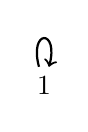
\begin{tikzpicture}
\node (atom1) {1};
\draw[->, thick] (atom1) to[loop above] (atom1);
\end{tikzpicture}\end{center}
However, since we want to make `$\exists x\forall yLxy$' \emph{false}, we need to make sure that for every $x$, there is at least one object it \emph{doesn't} bear $L$ to, i.e. we want the following to hold: $\forall x \exists y \enot Lxy$.  And the trouble is that as things stand, every object \emph{does} bear $L$ to something.

So let's try it with two objects.  Again, to make `$\forall xLxx$' true, they both need to bear $L$ to themselves:
\begin{center}\begin{tikzpicture}
\node (atom1) {1};
\node (atom2) [right=of atom1] {2};
\draw[->, thick] (atom1) to[loop above] (atom1);
\draw[->, thick] (atom2) to[loop above] (atom2);
\end{tikzpicture}\end{center}
Notice that at this point, `$\forall x \exists y \enot Lxy$' holds.  For every object we can find at least one thing it doesn't bear $L$ to: 1 doesn't bear $L$ to 2, and 2 doesn't bear $L$ to 1.  We still have to make sure that symmetry holds, i.e. that `$\forall x\forall y(Lxy \eif Lyx)$' is true.  But if you think about it, symmetry does hold in our diagram: everything that 1 bears $L$ to --- which is just itself --- also bears $L$ back to 1.  And similarly, everything that 2 bears $L$ to --- which is just itself --- also bears $L$ back to 2.  So we're done!  Our countermodel and accompanying semantic demonstration (which gets pretty involved in the case of symmetry!) looks like this:
\begin{center}
\begin{minipage}{0.8\textwidth}
\begin{multicols}{2}
\begin{ekey}
	\item[\text{Domain}] 1, 2
	\item[R] \ntuple{1,1}, \ntuple{2,2}
\end{ekey}
\columnbreak
\begin{tikzpicture}
\node (atom1) {1};
\node (atom2) [right=of atom1] {2};
\draw[->, thick] (atom1) to[loop above] (atom1);
\draw[->, thick] (atom2) to[loop above] (atom2);
\end{tikzpicture}
\end{multicols}\end{minipage}\end{center}

\begin{ebullet}
\item $\forall xLxx$ is true because:
\begin{etriangle}
\item $Lx^1x^1$ is true, and
\item $Lx^2x^2$ is also true
\end{etriangle}
\end{ebullet}

\begin{ebullet}
\item $\forall x\forall y(Lxy \eif Lyx)$ is true because:
\begin{etriangle}
\item $\forall y(Lx^1y \eif Lyx^1)$ is true, since:
\begin{itemize}
\item $(Lx^1y^1 \eif Ly^1x^1)$ is true (because $Lx^1y^1$ and $Ly^1x^1$ are both true), and
\item $(Lx^1y^2 \eif Ly^2x^1)$ is also true (because $Lx^1y^2$ is false)
\end{itemize}

\item and $\forall y(Lx^2y \eif Lyx^2)$ is true, since:
\begin{etriangle}
\item $(Lx^2y^1 \eif Ly^1x^2)$ is true (because $Lx^2y^1$ is false), and
\item $(Lx^2y^2 \eif Ly^2x^2)$ is also true (because $Lx^2y^2$ and $Ly^2x^2$ are both true)
\end{etriangle}
\end{etriangle}
\end{ebullet}

\begin{ebullet}
\item $\exists x\forall yLxy$ is false because:
\begin{etriangle}
\item $\forall y Lx^1y$ is false, since:
\begin{itemize}
\item $Lx^1y^2$ is false
\end{itemize}
\item and $\forall y Lx^2y$ is also false, since
\begin{etriangle}
\item $Lx^2y^1$ is false
\end{etriangle}
\end{etriangle}
\end{ebullet}

Again, the countermodel we arrived at is not the only one possible.  The following would work too, for example, and might be more intuitive:
\begin{center}
\begin{tikzpicture}
\node (atom1) {1};
\node (atom2) [right=of atom1] {2};
\node (atom3) [right=of atom2] {3};
\draw[->, thick] (atom1) to[loop above] (atom1);
\draw[->, thick] (atom2) to[loop above] (atom2);
\draw[->, thick] (atom3) to[loop above] (atom3);
\draw[->, thick] (atom1) to[bend right] (atom2);
\draw[->, thick] (atom2) to[bend right] (atom1);
\draw[->, thick] (atom2) to[bend right] (atom3);
\draw[->, thick] (atom3) to[bend right] (atom2);
\end{tikzpicture}
\end{center}
But with three objects in the domain, giving a semantic demonstration would require more work.  To show that `$\forall x\forall y(Lxy \eif Lyx)$' holds, for example, we'd have to show that `$\forall y(Lxy \eif Lyx)$' is true no matter which of our three objects we assign to `$x$'; and then relative to each choice for `$x$', we'd have to show that `$(Lxy \eif Lyx)$' is true no matter what we assign to `$y$'.  So we'd have to consider nine different assignments of objects to `$x$' and `$y$' in total, whereas the demonstration above only required us to look at four assignments.

\practiceproblems
\problempart Construct countermodels to demonstrate the following:

\begin{earg}

\item $\forall x \exists y Lxy \nvDash \exists x \forall y Lxy$ % Needs 2
\item $\forall x \exists yLyx \nvDash \forall x \exists yLxy$
\item $\exists x(Fx \eand \forall y Rxy) \nvDash \forall x(Fx \eif \exists yRxy)$ % Needs 2
\item $\exists x(\exists yAxy \eand \enot \exists y Ayx) \nvDash \exists x \forall y(Axy \eif Ayx)$
\item $\forall x(\forall yRxy \eif \exists z \forall wRwz) \nvDash \forall x \exists y \forall z(Rxy \eiff Rzy)$
\end{earg}


\section{Validity and Decidability}

Let's investigate one more argument involving a two-place predicate:
$$\forall x\exists yRxy, \forall x \forall y \forall z((Rxy \eand Ryz) \eif Rxz) \therefore \exists xRxx$$
For this to be valid, the seriality and transitivity of $R$ would together have to imply that some object bears $R$ to itself (again, there's no official name for this latter characteristic).  Let's see if we can construct a countermodel.

To make the conclusion `$\exists xRxx$' false, we have to make sure that \emph{no} object in our interpretation bears $R$ to itself, i.e. there can be no arrows that loop from an object onto itself.  And as we already noticed at the hand of Example 1 in the previous section, for seriality to hold in a domain of just one object, that object would have to bear the relation to itself.  So we cannot make seriality true and `$\exists xRxx$' false with just one object.

So let's move to a domain with two objects.  We can make seriality hold while avoiding any self-looping arrows like this:
\begin{center}
\begin{tikzpicture}
\node (atom1) {1};
\node (atom2) [right=of atom1] {2};

\draw[thick,->] (atom2) to[bend right] (atom1);
\draw[thick,->] (atom1) to[bend right] (atom2);
\end{tikzpicture}
\end{center}
But now consider how to make transitivity, i.e. `$\forall x \forall y \forall z((Rxy \eand Ryz) \eif Rxz)$', hold.  For this to be true, the conditional `$(Rxy \eand Ryz) \eif Rxz$' has to be true no matter which objects we assign to each of the variables `$x$', `$y$', and `$z$'. So suppose we assign  2 to `$y$', and 1 to both `$x$' and `$z$': $(Rx^1y^2 \eand Ry^2z^1) \eif Rx^1z^1$.  Both $Rx^1y^2$ and $Ry^2z^1$ are true, so for the latter conditional to be true, the consequent $Rx^1z^1$ has to be true.  But this would now require a self-looping arrow from $1$ back to $1$!  So we can't get what we want with just two objects.

Let's try three objects.  What we've just seen is that we can't have any symmetric arrows, since that would introduce a self-looping arrow by transitivity.  With three objects, we can secure seriality (making sure every object has an arrow going to some object) while avoiding both symmetric and self-looping arrows like this:
\begin{center}
\begin{tikzpicture}[>=stealth',thick]

\node (1) {1};
\node (2) [right=of 1] {2};
\node (3) [right=of 2] {3};

\draw[->,thick] (1) to (2);
\draw[->,thick] (2) to (3);
\draw[->,thick] (3) to[bend left] (1);

\end{tikzpicture}
\end{center}
But again, transitivity causes a problem.  Let's assign 2 to `$x$', 3 to `$y$', and 1 to `$z$', giving us: $(Rx^2y^3 \eand Ry^3z^1) \eif Rx^2z^1$.  Since both $Rx^2y^3$ and $Ry^3z^1$ are true, for the conditional to be true, the consequent $Rx^2z^1$ has to be true.   That would mean adding an arrow going from 2 to 1.  But since we already have an arrow going from 1 to 2,  that would reintroduce a double-headed arrow!

What this shows is that we can't have any arrows that ``go backward'' in our interpretation, to an earlier number.  We could add a fourth object so that 3's arrow can move forward:
\begin{center}
\begin{tikzpicture}[>=stealth',thick]

\node (1) {1};
\node (2) [right=of 1] {2};
\node (3) [right=of 2] {3};
\node (4) [right=of 3] {4};
\node (5) [below=1.5em of 4] {?};

\draw[->,thick] (1) to (2);
\draw[->,thick] (2) to (3);
\draw[->,thick] (3) to (4);
\draw[->,thick] (4) to[bend left] (5);

\end{tikzpicture}
\end{center}
But 4 \emph{also} has to have an arrow going to some object (for seriality).  And that arrow can't go backward to 1, 2, or 3, and can't go from 4 to itself, so what's to be done? Does this mean it's impossible to construct a countermodel, and that our argument is therefore valid?

No, it does not: the argument is invalid, and a countermodel exists, but it requires \emph{infinitely many objects} in its domain.  The following is a countermodel, for example:
\begin{ekey}
	\item[\text{Domain}] all positive integers
	\item[R] \blank \ is less than \blank \ (or: all pairs of integers \ntuple{m,n} where $m < n$)
\end{ekey}
We can't specify this interpreation ``directly'' by listing all the objects in the domain and all the pairs in the extension of `$R$', since there are too many of them.  But we can specify the extension of `$R$' indirectly, via the English predicate. This interpretation does what we want:
\begin{ebullet}
\item `$\forall x\exists yRxy$' is true, since for every positive integer $x$ we can find a $y$ such that $x<y$
\item `$\forall x \forall y \forall z((Rxy \eand Ryz) \eif Rxz)$' is true, since if $x < y$ and $y < z$, it follows that $x < z$.
\item `$\exists xRxx$' is false, since there exist no integer $x$ such that $x < x$.
\end{ebullet}

What we've seen, then, is that showing an FOL argument to be invalid may require an interpretation with infinitely many objects.  As mentioned in \S\ref{s:CountermodelOnePl}, this is not the case for FOL arguments that contain only \emph{one-place} predicates.  If such an argument is invalid, then there exists a countermodel with a domain of at most $2^n$ objects (where $n$ is the number of one-place predicates the argument contains).  Since there are finitely many interpretations for $n$ predicates using at most $2^n$ objects, this means that a computer could in principle crunch through all of those interpretations and determine if the argument is valid: if it finds a countermodel among them, the argument is invalid, if it doesn't, the argument is valid.

The same holds for TFL.  Any TFL argument can be tested for validity by constructing its joint truth table and checking wether any line (i.e. valuation) makes all the premises true and the conclusion false.  So a computer can be programmed to mechanically test any TFL argument for validity.

What we've seen is that this does not hold for FOL arguments that contain two-place predicates.  Here there is no finite number of interpretations we could program a computer to check such that, if it fails to find a countermodel among them, the argument is guaranteed to be valid.  And in fact, as the logicians Alan Turing and Alonzo Church independently proved in 1936, there exists \emph{no} mechanical test for validity in FOL. Validity in FOL is therefore said to be \define{undecidable}, in contrast to TFL, where validity is \define{decidable} via truth-tables.


Demonstrating FOL arguments to be valid therefore invariably requires some ingenuity and insight --- it's not the kind of thing a computer can do. This is why we use natural deduction proofs to demonstrate validity in FOL: if methods that require ingenuity are going to be required anyhow, we might as well use the method of natural deduction.\footnote{Of course, by using natural deductions to demonstrate validity, we are relying on the fact that our proof system is sound, i.e. only lets us prove valid arguments.  See the introduction to Chapter \ref{ch:NDFOL} on this concept.}
To be sure, one \emph{can} also give semantic proofs to demonstrate the validity of FOL arguments.  For example to show that the following entailment holds:
$$\exists x(Fx \eand Gx) \vDash \exists x Fx \eand \exists xGx$$
we could give the following semantic proof in English:
\begin{itemize}
\item[] \emph{Semantic Proof:} consider some arbitrary interpretation \meta{I}, and suppose $\exists x(Fx \eand Gx)$ is true in \meta{I}.  This means there is some object in the domain of \meta{I}, let's call it $a$, such that $(Fx^a \eand Gx^a)$ is true in \meta{I}.  But then since $Fx^a$ is true in \meta{I}, this means $\exists xFx$ is true in \meta{I}.  And similarly, since $Gx^a$ is true in \meta{I}, it follows that $\exists xGx$ must be true in \meta{I}.  Therefore $\exists x Fx \eand \exists xGx$ is true in \meta{I}.  Since \meta{I} was an arbitrary interpretation, we can conclude that \emph{every} interpretation that makes $\exists x(Fx \eand Gx)$ true must also make $\exists x Fx \eand \exists xGx$ true, meaning that the entailment above holds.
\end{itemize}
However, we can also give a natural deduction proof, which goes through a very similar line of reasoning:
\begin{proof}
	\hypo{1}{\exists x (Fx \eand Gx)} \by{Premise}{}
	\open
		\hypo{2}{Fa \eand Ga} \by{Assumption (flag a)}{}
		\have{3}{Fa}\ae{2}
		\have{4}{\exists xFx} \Ei{3}
		\have{5}{Ga}\ae{2}
		\have{6}{\exists xFx} \Ei{5}
		\have{7}{\exists xFx \eand \exists xGx} \ai{4,6}
	\close
	\have{7}{\exists xFx \eand \exists xGx} \Ee{1,2-7}
\end{proof}
Natural deduction proofs do not, however, allow use to demonstrate that arguments are \emph{invalid}.  To do this, we have to rely on the method of constructing countermodels.  And that's what we have been doing in the last several sections.


\section{Working with Other Semantic Concepts}


So far, we've just been focusing on validity, or entailment. But we can use interpretations, as well as natural deduction proofs, in connection with other semantic concepts too.

Take the concept of logical truth first.  To show that some FOL sentence \meta{\varphi} is \emph{not} a logical truth, it suffices to construct an interpretation that makes it false.  And to show that it \emph{is} a logical truth, we can give a natural deduction that proves \meta{\varphi} as a theorem.  This gives us a way to approach contradictions as well: since \meta{\varphi} is a contradiction iff $\enot\meta{\varphi}$ is a logical truth, we can show that \meta{\varphi} is a contradiction by proving $\enot\meta{\varphi}$ as a theorem.  And to show that \meta{\varphi} is \emph{not} a contradiction, it suffices to construct an interpretation in which it is true.


Next consider logical equivalence.  To show that \meta{\varphi} and \meta{\psi} are \emph{not} logically equivalent, all we need to do is construct an interpretation on which one of them is true and the other is false.  And to show that \meta{\varphi} and \meta{\psi} \emph{are} equivalent, we can give a natural deduction that proves $\meta{\varphi} \eiff \meta{\psi}$ as a theorem, since \meta{\varphi} and \meta{\psi} are equivalent just in case $\meta{\varphi} \eiff \meta{\psi}$ is a logical truth.


Lastly, take the concept of consistency.  To show that some sentences are jointly consistent, it suffices to give an interpretation on which they are all true.  As for inconsistency, notice that it connects to entailment in the following way:
\factoidbox{$$\text{If } \meta{\varphi}_1, \ldots, \meta{\varphi}_n \entails \bot \text{, then } \meta{\varphi}_1, \ldots, \meta{\varphi}_n \text{ are jointly inconsistent} $$
}
For suppose  $\meta{\varphi}_1, \ldots, \meta{\varphi}_n \entails \bot$.  This means there's no interpretation that makes all of $\meta{\varphi}_1, \ldots, \meta{\varphi}_n $ true but $\bot$ false.  However, since every interpretation makes $\bot$ false, this just means that there's no interpretation that makes all of $\meta{\varphi}_1, \ldots, \meta{\varphi}_n $ true.  That is, $\meta{\varphi}_1, \ldots, \meta{\varphi}_n $ are inconsistent.    So if we want to show that $\meta{\varphi}_1, \ldots, \meta{\varphi}_n $ are inconsistent, we can do that by giving a natural deduction proof showing that $\meta{\varphi}_1, \ldots \meta{\varphi}_n \proves \bot $.

The following table summarizes what is needed to demonstrate that a given concept does or does not apply:
\begin{center}
\begin{tabular}{l l l}
%\cline{2-3}
 & \textbf{Yes} & \textbf{No}\\
 \hline
%\cline{2-3}
logical truth? & give a proof & give an interpretation\\
contradiction? &  give a proof  & give an interpretation\\
equivalent? & give a proof & give an interpretationl\\
consistent? & give an interpretation & give a proof\\
valid? & give a proof & give an interpretation\\
entailment? & give a proof & give an interpretation\\
\end{tabular}
\end{center}


\practiceproblems

%\problempart
%Give counermodels to show the following:
%
%\begin{earg}
%\item $\forall x(Ax \eif Bx) \nvDash \exists x Bx$
%\item $\forall x(Rx \eif Dx), \forall x(Rx \eif Fx) \nvDash \exists x(Dx \eand Fx)$
%\item $\exists x(Px\eif Qx) \nvDash \exists x Px$
%\item $Na \eand Nb \eand Na \nvDash \forall x Nx$
%\item $\exists x(Ex \eand Fx), \exists x Fx \eif \exists x Gx \nvDash \exists x(Ex \eand Gx)$
%\item $Rab, \exists x Rxa \nvDash Rba$
%\item $\forall x Oxa, \forall x Oax \nvDash \forall x Oxx$
%\item $\forall x \exists yLxy \nvDash \exists x \forall yLxy$
%\item $\exists x(Jx \eand Kx), \exists x \enot Kx, \exists x \enot Jx \nvDash \exists x(\enot Jx \eand \enot Kx)$
%\item $Lab \eif \forall x Lxb, \exists x Lxb \nvDash Lbb$
%\item $\forall x(Dx \eif \exists y Tyx) \nvDash \exists y \exists z\  y \neq z$
%\item $\forall x (Fx \eor \enot Gx) \nvDash (\forall x Fx \eor \enot \exists x Gx)$
%\item $\forall x\exists y(Rxy \eif Rxx) \nvDash \forall x(\exists yRxy \eif Rxx)$
%\item $\forall xFx \eiff \forall yGy \nvDash \forall x(Fx \eiff AyGy)$
%\item $\forall x \exists yRxy , \exists x\forall yRxy \nvDash \forall x \forall y Rxy$
%\item $\nvDash \exists x \forall y((Rxy \land \sim Ryx) \rightarrow (Rxx \leftrightarrow Ryy))$
%\end{earg}

%\problempart
%\label{pr.Contingent}
%Show that each of the following is neither a logical truth nor a contradiction (by constructing an interpretation for each that makes it true, and one that makes it false):
%\begin{earg}
%\item  $Da \eand Db$
%\item  $\exists x Txh$
%\item  $Pa \eand \enot\forall x Px$
%\item $\forall z Jz \eiff \exists y Jy$
%\item $\forall x (Rxa \eor \exists yLxy)$
%\item $\exists x (Gx \eif \forall y My)$
%%\item $\exists x (x = h \eand x = i)$
%\item $\exists x \forall y((Rxy \eand \enot Ryx) \eif (Rxx \eiff Ryy))$
%\end{earg}

\problempart
\label{pr.NotEquiv}
Show that the following pairs of sentences are not logically equivalent (by constructing an interpretation for each pair that makes one true but the other false):
\begin{earg}
\item $\exists x Jx$, $\exists x \lnot Jx$
\item $\exists x Jx \land \exists x Hx, \exists x(Jx \land Hx)$
\item $\forall x Rxx$, $\exists x Rxx$
\item $\exists x Px \eif \exists yQy$, $\exists x (Px \eif \exists yQy)$
\item $\forall x(Px \eif \enot Qx)$, $\exists x(Px \eand \enot Qx)$
\item $\exists x(Px \eand Qx)$, $\exists x(Px \eif Qx)$
\item $\forall x(Px\eif Qx)$, $\forall x(Px \eand Qx)$
\item $\forall x\exists y Rxy$, $\exists x\forall y Rxy$
\item $\forall x\exists y Rxy$, $\forall x\exists y Ryx$
\end{earg}



\problempart
Show that the following sentences are jointly consistent (i.e. there's an interpretation that makes them all true):
\begin{earg}
%\item $Ma, \enot Na, Pa, \enot Qa$
%\item $La, Lab, \enot Lbe, \enot Lbb$
%\item $\enot (Ma \eand \exists x Ax), Ma \eor Fa, \forall x(Fx \eif Ax)$
%\item $Ma \eor Mb, Ma \eif \forall x \enot Mx$
\item $\forall y Gy, \forall x (Gx \eif Hx), \exists y \enot Iy$
\item $\exists x(Bx \eor Ax), \forall x \enot Cx, \forall x\bigl[(Ax \eand Bx) \eif Cx\bigr]$
\item $\exists x Xx, \exists x Yx, \forall x(Xx \eiff \enot Yx)$
\item $\forall x(Px \eor Qx), \exists x\enot(Qx \eand Px)$
\item $\exists z(Nz \eand Ozz), \forall x\forall y(Oxy \eif Oyx)$
\item $\enot \exists x \forall y Rxy, \forall x \exists y Rxy$
%\item $\enot Raa$, $\forall x (x=a \eor Rxa)$
%\item $\forall x\forall y\forall z(x=y \eor y=z \eor x=z)$, $\exists x\exists y\ \enot x= y$
%\item $\exists x\exists y(Zx \eand Zy \eand x=y)$, $\enot Zd$, $d=e$
\end{earg}

%\problempart
%\label{pr.FOLequivornot}
%For each of the following pairs of sentences, if they are provably equivalent, give proofs to show this, and if they are not, construct countermodel to show they are not equivalent:
%\begin{earg}
%\item $\forall x Px \eif \exists yQy, \forall x (Px \eif \exists yQy)$
%\item $\forall x\forall y \forall z Bxyz, \forall x Bxxx$
%\item $\forall x\forall y Dxy, \forall y\forall x Dxy$
%\item $\exists x\forall y Dxy, \forall y\exists x Dxy$
%\item $\forall x (Rba \eiff Rxa), Rba \eiff \forall x Rxa$
%\end{earg}

%\problempart
%\label{pr.FOLvalidornot}
%For each of the following arguments: if it is valid in FOL, give a proof. If it is invalid, construct an interpretation to show that it is invalid.
%\begin{earg}
%\item $\exists y\forall x Rxy \therefore \forall x\exists y Rxy$
%\item $\exists x(Px \eand \enot Qx) \therefore \forall x(Px \eif \enot Qx)$
%\item $\forall x(Sx \eif Ta), Sb \therefore Ta$
%\item $\forall x(Ax\eif Bx), \forall x(Bx \eif Cx) \therefore \forall x(Ax \eif Cx)$
%\item $\exists x(Dx \eor Ex), \forall x(Dx \eif Fx) \therefore \exists x(Dx \eand Fx)$
%\item $\forall x\forall y(Rxy \eor Ryx) \therefore Raa$
%\item $\exists x\exists y(Rxy \eor Ryx) \therefore Raa$
%\item $\forall x Px \eif \forall x Qx, \exists x \enot Px \therefore \exists x \enot Qx$
%\end{earg}


\section{Semantics for Identity}

As mentioned in  \S\ref{s:identity}, FOL is standardly supplemented with a primitive logical symbol $=$ for \emph{identity}. In \S\ref{s:identityrules} we looked at the deduction rules that govern identity, with which we were then able to prove various logical truths involving identity, like that everything is identical to itself, $\forall x  \ x=x$.

Similarly, we now need to say something about the semantics of identity, specifically how to determine the truth values of identity statements in an interpretation.  In this case, the semantics is very simple:%\footnote{This clause assumes that variables can refer to objects, but technically variables only refer \emph{relative to} an assignment of values.  Again, see the Appendix in \S\ref{s:semanticsappendix} below for the official semantics, that makes the role of variable assignments explicit.}
\factoidbox{
		For any names $\meta{a}$ and $\meta{b}$, $\meta{a} = \meta{b}$ is true in a given interpretation \textbf{iff}  \meta{a} and \meta{b} refer to very same object in that interpretation.
}
So if, for example, our interpretation specifies that the name `$m$' refers to 1, that `$n$' refers to 2, and that `$o$' also refers to 2, then `$m = n$' would be false (since 1 and 2 aren't identical) whereas `$n = o$' would be true (since 2 is identical to 2).  And of course, things like `$m = m$' or `$n = n$' will always be true, on any interpretation, since \emph{whatever} `$n$' (or `$m$') refers to, it will be identical to itself.


This clause only covers identity statements involving names.  For identity statements involving variables, we again have to bring in variable assignments.  E.g. `$x=y$' comes out true if the variables `$x$' and `$y$' are both assigned the value 1, say, but it would come out false if `$x$' were assigned the value 1 and `$y$' the value $2$.  On the other hand, `$x=x$' comes out true no matter what value is assigned to `$x$'.  See the Appendix in \S\ref{s:semanticsappendix} below for the official semantics that makes the role of variable assignments explicit.


We can also consider quantified sentences involving identity.  In \S\ref{s:identity} we saw how to symbolize numerical claims using identity.  The claim that exactly one object exists can, for example, be symbolized as `$\exists x \forall y \ x = y$', and the claim that exactly two objects exist can be symbolized as `$\exists x \exists y( x \neq y \eand \forall z(z = x \eor z = y))$'.\footnote{Again, $x \neq y$ is jus shorthand for $\enot (x = y)$}   Using our semantics, we can now show that `$\exists x \forall y \ x = y$' is indeed false if the domain contains more than one object:

\begin{center}

\begin{ekey}
	\item[\text{Domain}] 1, 2
\end{ekey}
\end{center}

\begin{ebullet}
\item[] $\exists x \forall y \ x = y$ is false because:
\begin{etriangle}
\item $\forall y \ x^1 = y$ is false
\begin{etriangle}
\item since $x^1 = y^2$ is false.
\end{etriangle}
\item and $\forall y \ x^2 = y$ is also false
\begin{etriangle}
\item since $x^2 = y^1$ is false.
\end{etriangle}
\end{etriangle}
\end{ebullet}
Similarly, we could show that `$\exists x \exists y( x \neq y \eand \forall z(z = x \eor z = y))$', that is, the claim that exactly two objects exist, is false on a domain that contains 1, 2, and 3. (Though for this, the complete semantic demonstration would be quite long, since there are three possible values to consider for `$x$', and then three possible values for `$y$' in each case!)


\practiceproblems

\problempart Consider again the following interpretation:

\begin{multicols}{2}
	\begin{ekey}
		\item[\text{Domain}] 1, 2, 3
		\item[R] \ntuple{1,3}, \ntuple{2,2}, \ntuple{2,3}, \ntuple{3, 2} \ntuple{3,3}
	\end{ekey}
\columnbreak

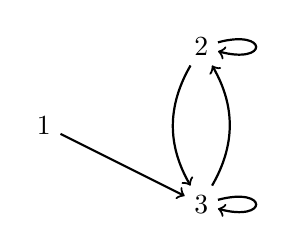
\begin{tikzpicture}
\node (atom1) at (0,1) {1};
\node (atom2) at (2,2) {2};
\node (atom3) at (2,0) {3};
\draw[->, thick] (atom1)--(atom3);
\draw[->, thick] (atom2) to[bend right] (atom3);
\draw[->, thick] (atom3) to[bend right] (atom2);
\draw[->, thick] (atom3) to[loop right, looseness=15] (atom3);
\draw[->, thick] (atom2) to[loop right, looseness=15] (atom2);
%\draw[->, thick] (atom4) to[loop right, looseness=15] (atom4);
\end{tikzpicture}

\end{multicols}


\noindent Determine whether each of the following sentences is true or false in this interpretation, and give a semantic demonstration to justify your answer.
\begin{earg}
\item $\forall x (\exists y \ x \neq y \eand \exists y \ x = y)$
\item $\forall x \exists y ( x \neq y \eand \ x = y)$
\item $\exists x \forall y \ x = y$
\item $\exists x \exists y (x \neq y \eand  (Rxy \eand Ryx))$
\item $\exists x \forall y(Rxy \eiff x = y)$
\item $\exists x \forall y(Ryx \eiff x = y)$
\item $\exists x \exists y((x \neq y \eand Rxy) \eand \forall z(Rzx \eiff y = z))$
\end{earg}


\problempart
\label{pr.Contingent}
Show that each of the following is neither a logical truth nor a contradiction:
\begin{earg}
\item $\forall x \exists y \ x \neq y$
\item $\exists x (x = a \eand x = b)$
\item $\forall x \forall y \forall z((x = y \eor x = z) \eor y = z)$
\item $\exists x \exists y \ x \neq y$
\end{earg}
Show that the following sentences are jointly consistent (i.e. there's an interpretation that makes them all true):
\begin{earg}
\setcounter{eargnum}{4}
\item $\enot Raa$, $\forall x (x=a \eor Rxa)$
\item $\forall x\forall y\forall z(x=y \eor y=z \eor x=z)$, $\exists x\exists y\ \enot x= y$
\item $\exists x\exists y(Zx \eand Zy \eand x=y)$, $\enot Za$, $a=b$
\end{earg}







\section{Appendix: Semantics with Variable Assignments}\label{s:semanticsappendix}

In \S\ref{s:TruthQuantifiedSentences} we explained the semantics for quantifiers using the notion of a variable assignment: an assignment of an object to a variable, representing our decision to temporarily treat the variable as if it referred to that object.  However, once we introduce variable assignments to deal with quantifiers, we should really go back and re-do our semantics with variable assignments in mind from the beginning, even when we're just looking at atomic sentences.


To see why, consider a simple example like `$\forall xFx$', and suppose our domain contains just the numbers 1 and 2.  Then in order for `$\forall xFx$' to be true, the formula `$Fx$' needs to be true on the assignment $[x:1]$ and also on $[x:2]$.  But what is required for `$Fx$' to be true on $[x:1]$, say?  The answer, of course, is that `$F$' has to be true of 1, the object we're treating `$x$' as referring to.  But the semantics we gave for atomic sentences doesn't \emph{technically} tell us this!  What we said in \S\ref{s:TruthFOL} was just the following:
	\factoidbox{
		When \meta{R} is an $n$-place predicate and $\meta{c}_1, \meta{c}_{2}, \ldots, \meta{c}_{n}$ are names, the sentence $\meta{R}\meta{c}_{1}\meta{c}_{2}\ldots\meta{c}_{n}$ is true in a given interpretation \textbf{iff} $\meta{R}$ is true of the objects referred to by $\meta{c}_{1}, \meta{c}_{2}, \ldots, \meta{c}_{n}$ (in that order) in that interpretation	}
This doesn't mention variable assignments anywhere.  And furthermore, it only deals with atomic \emph{sentences}, things that only contain \emph{names}.  `$Fx$'  contains a variable instead of a name.  It is merely a \emph{formula}, so the above explanation simply does not apply to it.

To remedy this situation, we need to return to the official explanation of the syntax, or grammar, of FOL that we gave way back in \S\ref{s:FOLSyntax}.  Recall that we there defined the general class of \emph{formulas} of FOL, among which we then singled out the smaller class of FOL \emph{sentences}.  We did this in four steps.  First, we stipulated that a \define{term} is to be any name \emph{or any variable}.  Second, we said that an \define{atomic formula} is anything that results from combining any predicate (including the identity symbol) with an appropriate number of \emph{terms}. Third, we said that a \define{formula}, more generally, is anything that can be built up from atomic formulas using truth functional operators and quantifiers.  And lastly, we then said that a \define{sentence} is any formula that contains no free, or unbound, variables.

We here have to do something similar.  We will first have to give a general explanation of truth that covers all \emph{formulas}, such as `$Fx$', and then extract from that a notion of truth for just \emph{sentences}.  In particular, what we'll do is to explain what is required for any formula whatsoever to be true in an interpretation \emph{relative to a variable assignment}.  In what follows, let's use \script{I} for an arbitrary interpretation, and $[ ]$ for an arbitrary variable assignment.  So we will give a general explanation of what is required for any \emph{formula} to be \emph{true on $[]$ in \script{I} }.  Later we'll then use that to say what's required for a \emph{sentence} to be true in an interpretation.

To begin, we first give an expanded notion of reference that covers both names (like $a, b, c \ldots$) and variables (like $x, y, z \ldots$).  Again: a variable doesn't actually refer to anything, since it isn't a name.  But  \emph{relative to a variable assignment}, variables can be construed as referring to things.  So:
\factoidbox{
For any term \meta{t} (name or variable), the \define{referent of \meta{t} on [] in}  \script{I}  is:
\begin{etriangle}
\item whatever object the interpretation \script{I} assigns to \meta{t}, if \meta{t} is a name, and
\item whatever object the assignment [] assigns to \meta{t}, if \meta{t} is a variable
\end{etriangle}
}

We can now use this expanded notion of reference to explain truth for all atomic formulas, whether they contain names or variables:


\factoidbox{
		When \meta{R} is an $n$-place predicate and $\meta{t}_1, \ldots, \meta{t}_{n}$ are any terms (names \emph{or} variables), the formula $\meta{R}\meta{t}_{1} \ldots\meta{t}_{n}$ is true on [] in \script{I}  \textbf{iff} $\meta{R}$ is true of the objects referred to by $\meta{t}_{1},  \ldots, \meta{t}_{n}$ (in that order) on [] in \script{I}.	\\

And for any terms $\meta{t}_1$ and $\meta{t}_2$, the formula $\meta{t}_1 = \meta{t}_2$ is true on [] in \script{I}  iff $\meta{t}_1$ and $\meta{t}_2$ refer to the same thing on [] in \script{I}.
		}

This now \emph{does} specify what's required for e.g. `$Fx$' to be true on $[x:1]$.  What's required is that `$F$' be true of the referent of `$x$' on $[x:1]$.  And the referent of `$x$' on this assignment is of course just 1, give our expanded notion of reference.  So `$F$' has to be true of 1.  With atomic formulas covered, we can go on to explain truth for all complex formulas:
\factoidbox{
$\enot \meta{\varphi}$ is true on [] in \script{I}  \textbf{iff} $\meta{\varphi}$ false on [] in \script{I} \\

$\meta{\varphi} \eand \meta{\psi}$ is true on [] in \script{I} \textbf{iff} both $\meta{\varphi}$ and $\meta{\psi}$ are true on [] in \script{I} \\

$\meta{\varphi} \eor \meta{\psi}$ is true on [] in \script{I}  \textbf{iff} either $\meta{\varphi}$ or $\meta{\psi}$ are true on [] in \script{I} \\

$\meta{\varphi} \eif \meta{\psi}$ is true on [] in \script{I} \textbf{iff} either $\meta{\varphi}$ is false or $\meta{\psi}$ is true on [] in \script{I}\\

$\meta{\varphi} \eiff \meta{\psi}$ is true on [] in \script{I} \textbf{iff} $\meta{\varphi}$ and $\meta{\psi}$ have the same truth value on [] in \script{I}\\

$\forall \meta{v}\meta{\varphi}(\ldots \meta{v} \ldots)$ is true on [] in \script{I}  \textbf{iff} for \emph{every object} $o$ in the domain, $\meta{\varphi}(\ldots \meta{v} \ldots)$ is true on [\meta{v}:o] in \script{I}\\

$\exists \meta{v}\meta{\varphi}(\ldots \meta{v} \ldots)$ is true on [] in \script{I}  \textbf{iff} for \emph{at least one object} $o$ in the domain, $\meta{\varphi}(\ldots \meta{v} \ldots)$ is true on [\meta{v}:o] in \script{I}.
}
In the claues governing the quantifiers, [\meta{v}:o] is the assignment that's just like our arbitrary assignment [] in every respect, except that it is stipulated to assign the object $o$ to the variable \meta{v}.  The idea, again, being that we go through each object $o$ in the domain, and check whether the formula $\meta{\varphi}(\ldots \meta{v} \ldots)$ is true when that object $o$ is assigned to the variable \meta{v}.  If so, $\forall \meta{v}\meta{\varphi}(\ldots \meta{v} \ldots)$ is true, if not, it is false.  On the other hand, for an existential sentence $\exists \meta{v}\meta{\varphi}(\ldots \meta{v} \ldots)$ to be true, it's enough if \emph{at least one} object makes $\meta{\varphi}(\ldots \meta{v} \ldots)$ true.

Given all of this, we can now say what is required for any \emph{sentence}, i.e. any closed formula, or formula with no free variables, to be true in an interpretation \script{I}:

\factoidbox{For any FOL sentence \meta{\varphi} and any interpretation \script{I}, \meta{\varphi} is true in \script{I} iff \meta{\varphi} is true in \script{I} on \emph{any assignment [] whatsoever}.
}
With this explanation of truth for sentences in place, the definition of the various logical concepts (like entailment, logical truth, equivalence etc.) now proceeds as it did in \S\ref{s:FOLSemanticConcepts}.
\chapter[Quick Reference]{Quick Reference}
%\pagestyle{plain}
\section*{Truth Functional Operators (Ch. \ref{ch:SemanticsOfTFL})}


\begin{center}
\begin{tabular}{c c|c|c|c|c|c}
\meta{\varphi} & \meta{\psi} & $\enot \meta{\varphi}$ & $\meta{\varphi}\eand\meta{\psi}$ & $\meta{\varphi}\eor\meta{\psi}$ & $\meta{\varphi}\eif\meta{\psi}$ & $\meta{\varphi}\eiff\meta{\psi}$\\
\hline
T & T & F & T & T & T & T\\
T & F & F & F & T & F & F\\
F & T & T & F & T & T & F\\
F & F & T & F & F & T & T
\end{tabular}
\end{center}



%\section{Symbolisation}
%\begin{center}
%\label{app.symbolization}
%\begin{tabular*}{\textwidth}{rl}
%\multicolumn{2}{c}{\textsc{Sentential Connectives}}\\ \\
%It is not the case that P & $\enot P$\\
%Either P, or Q & $(P \eor Q)$\\
%Neither P, nor Q & $\enot(P \eor Q)$\ or \ $(\enot P \eand \enot Q)$\\
%Both P, and Q & $(P \eand Q)$\\
%If P, then Q & $(P \eif Q)$\\
%P only if Q & $(P \eif Q)$\\
%P if and only if Q & $(P \eiff Q)$\\
%P unless Q & $(P \eor Q)$\\
%\\
%\multicolumn{2}{c}{\label{SymbolizingPredicates}\textsc{Predicates}}\\ \\
%All Fs are Gs & $\forall x(Fx \eif Gx)$\\
%Some Fs are Gs & $\exists x(Fx \eand Gx)$\\
%Not all Fs are Gs & $\enot\forall x(Fx \eif Gx)$\ or\ $\exists x(Fx \eand \enot Gx)$\\
%No Fs are Gs & $\forall x(Fx \eif\enot Gx)$\ or\ $\enot\exists x(Fx \eand Gx)$\\
%\\
%\multicolumn{2}{c}{\textsc{Identity}}\\ \\
%Only c is G & $\forall x(Gx \eiff x=c)$\\
%Everything besides c is G & $\forall x(\enot x = c \eif Gx)$\\
%%$j$ is more $R$ than anyone else. & $\forall x(x\neq j \eif Rjx)$\\
%The F is G & $\exists x(Fx \eand \forall y(Fy \eif x=y) \eand Gx)$\\
%It is not the case that the F is G & $\enot\exists x(Fx \eand \forall y(Fy \eif x=y) \eand Gx)$\\
%The F is non-G & $\exists x(Fx \eand \forall y(Fy \eif x=y) \eand \enot Gx)$
%\end{tabular*}
%\end{center}
%
%
%
%
%
%
%% BEGIN: symbolizing cardinality
%
%\newpage
%\section{Using identity to symbolize quantities}
%
%\subsection*{There are at least \blank\ Fs.}
%\label{summary.atleast}
%
%\begin{ekey}
%\item[\text{one}] $\exists xFx$
%\item[\text{two}] $\exists x_1\exists x_2(Fx_1 \eand Fx_2 \eand \enot x_1  = x_2)$
%\item[\text{three}] $\exists x_1\exists x_2\exists x_3(Fx_1 \eand Fx_2 \eand Fx_3 \eand \enot x_1 = x_2 \eand\enot x_1 = x_3 \eand \enot x_2 = x_3)$
%\item[\text{four}] $\exists x_1\exists x_2\exists x_3\exists x_4 (Fx_1 \eand Fx_2 \eand Fx_3 \eand Fx_4 \eand \phantom{x}$\\
%\phantom{$\exists x_1\exists x_2$}$\enot x_1 = x_2 \eand \enot x_1 = x_3 \eand \enot x_1 = x_4 \eand \enot x_2 = x_3 \eand \enot x_2 = x_4 \eand \enot x_3 = x_4)$
%\item[n] $\exists x_1\ldots\exists x_n(Fx_1 \eand\ldots\eand Fx_n \eand \enot x_1 = x_2 \eand\ldots\eand \enot x_{n-1} = x_n)$
%\end{ekey}
%
%\subsection*{There are at most \blank\ Fs.}
%\label{summary.atmost}
%
%One way to say `there are at most $n$ Fs' is to put a negation sign in front of the symbolisation for `there are at least $n+1$ Fs'. Equivalently, we can offer:
%\begin{ekey}
%\item[\text{one}] $\forall x_1\forall x_2\bigl[(Fx_1 \eand Fx_2) \eif x_1=x_2\bigr]$
%\item[\text{two}] $\forall x_1\forall x_2\forall x_3\bigl[(Fx_1 \eand Fx_2 \eand Fx_3) \eif (x_1=x_2 \eor x_1=x_3 \eor x_2=x_3)\bigr]$
%\item[\text{three}] $\forall x_1\forall x_2\forall x_3\forall x_4\bigl[(Fx_1 \eand Fx_2 \eand Fx_3 \eand Fx_4) \eif \phantom{.}$\\
%\phantom{$\exists x_1 \exists x_2$}$(x_1=x_2 \eor x_1=x_3 \eor x_1=x_4 \eor x_2=x_3 \eor x_2=x_4 \eor x_3=x_4)\bigr]$
%\item[n]$\forall x_1\ldots\forall x_{n+1}
%\bigl[(Fx_1\eand \ldots \eand Fx_{n+1}) \eif (x_1=x_2 \eor \ldots \eor x_n=x_{n+1})\bigr]$
%\end{ekey}
%
%\subsection*{There are exactly \blank\ Fs.}
%\label{summary.exactly}
%
%One way to say `there are exactly $n$ Fs' is to conjoin two of the symbolizations above and say `there are at least $n$ Fs and there are at most $n$ Fs.' The following equivalent formulae are shorter:
%\begin{ekey}
%\item[\text{zero}] $\forall x\enot Fx$
%\item[\text{one}] $\exists x\bigl[Fx \eand \forall y(Fy \eif x= y)\bigr]$
%\item[\text{two}] $\exists x_1\exists x_2\bigl[Fx_1 \eand Fx_2 \eand \enot x_1 = x_2 \eand \forall y\bigl(Fy \eif (y= x_1 \eor y = x_2)\bigr) \bigr]$
%\item[\text{three}] $\exists x_1\exists x_2\exists x_3\bigl[Fx_1 \eand Fx_2 \eand Fx_3 \eand \enot x_1 =  x_2 \eand \enot  x_1 = x_3 \eand \enot x_2 = x_3 \eand \phantom{.}$\\
%\phantom{$\exists x_1 \exists x_2$}$\forall y\bigl(Fy \eif (y = x_1 \eor y = x_2 \eor y =  x_3)\bigr) \bigr]$
%\item[n] $\exists x_1\ldots\exists x_n\bigl[Fx_1 \eand\ldots\eand Fx_n  \eand \enot x_1 = x_2 \eand\ldots\eand \enot x_{n-1}= x_n \eand \phantom{.}$\\
%\phantom{$\exists x_1\exists x_2$}$\forall y\bigl(Fy \eif (y= x_1 \eor \ldots \eor y= x_n)\bigr)\bigr]$
%%\item[one] $\exists x\forall y\bigl[Fx \eand (Fy \eif y = x)\bigr]$
%%\item[two] $\exists x\exists y\forall z\Bigl(Fx \eand Fy \eand \bigl[Fz \eif (z=x \eor z=y)\bigr] \eand x \neq y\Bigr)$
%%\item[three] $\exists x_1\exists x_2\exists x_3\forall y\Bigl(Fx_1 \eand Fx_2 \eand Fx_3 \eand [Fy \eif (y=x_1 \eor y=x_2 \eor y=x_3)] \eand x_1 \neq x_2 \eand x_1 \neq x_3 \eand x_2 \neq x_3\Bigr)$
%%\item[n] $\exists x_1\cdots\exists x_n\forall y\Bigl(Fx_1 \eand\cdots\eand Fx_n \eand \bigl[Fy \eif (y=x_1 \eor \cdots \eor y=x_n)\bigr] \eand x_1 \neq x_2 \eand\cdots\eand x_{n-1}\neq x_n\Bigr)$
%\end{ekey}
%



\section*{Deduction Rules for TFL (Ch. \ref{ch:NDTFL})}
\renewenvironment{proof}
	{\noindent\par\noindent\small$\begin{nd}}
	{\end{nd}$\noindent\normalsize\ignorespacesafterend}

%{\LARGE \textbf{Basic Rules of Proof}}
\begin{multicols}{2}

\noindent\textbf{Conjunction Introduction}

\begin{proof}
	\have[m]{a}{\meta{\varphi}}
	\have[n]{b}{\meta{\psi}}
	\have[\ ]{c}{\meta{\varphi}\eand\meta{\psi}} \ai{a, b}
\end{proof}


\vspace{1em}\noindent\textbf{Conjunction Elimination}

\begin{proof}
	\have[m]{ab}{\meta{\varphi}\eand\meta{\psi}}
\\	\have[\ ]{a}{\meta{\varphi}} \ae{ab}

	\have[m]{ab}{\meta{\varphi}\eand\meta{\psi}}
\\	\have[\ ]{b}{\meta{\psi}} \ae{ab}
\end{proof}

\vspace{1em}\noindent\textbf{Conditional Introduction}

\begin{proof}
	\open
	\hypo[i]{a}{\meta{\varphi}} \by{Assumption}{}
	\have[j]{b}{\meta{\psi}}
	\close
	\have[\ ]{ab}{\meta{\varphi}\eif\meta{\psi}}\ci{a-b}
\end{proof}

\columnbreak
\vspace{1em}\noindent\textbf{Conditional Elimination}

\begin{proof}
	\have[m]{ab}{\meta{\varphi}\eif\meta{\psi}}
	\\	\have[n]{a}{\meta{\varphi}}
	\have[\ ]{b}{\meta{\psi}} \ce{ab,a}
\end{proof}

\vspace{1em}\noindent\textbf{Biconditional Introduction}

\begin{proof}
	\open
		\hypo[i]{a1}{\meta{\varphi}} \by{Assumption}{}
		\have[j]{b1}{\meta{\psi}}
	\close
	\open
		\hypo[k]{b2}{\meta{\psi}}\by{Assumption}{}
		\have[l]{a2}{\meta{\varphi}}
	\close
	\have[\ ]{ab}{\meta{\varphi}\eiff\meta{\psi}}\bi{a1-b1,b2-a2}
\end{proof}

\vspace{1em}\noindent\textbf{Biconditional Elimination}
\begin{proof}
	\have[m]{ab}{\meta{\varphi}\eiff\meta{\psi}}
\\	\have[n]{a}{\meta{\varphi}}
	\have[\ ]{b}{\meta{\psi}} \be{ab,a}
\end{proof}

\end{multicols}

\newpage
\begin{multicols}{2}
\begin{proof}
	\have[m]{ab}{\meta{\varphi}\eiff\meta{\psi}}
\\	\have[n]{a}{\meta{\psi}}
	\have[\ ]{b}{\meta{\varphi}} \be{ab,a}
\end{proof}



\vspace{1em}\noindent\textbf{Negation Introduction}

\begin{proof}
	\open
	\hypo[m]{a}{\meta{\varphi}} \by{Assumption}{}
	\have[n]{nb}{\ered}
	\close
	\have[\ ]{na}{\enot\meta{\varphi}}\ni{a-nb}
\end{proof}


\vspace{1em}\noindent\textbf{Negation Elimination}

\begin{proof}
	\have[m]{a}{\meta{\varphi}}
	\have[n]{na}{\enot\meta{\varphi}}
	\have[ ]{bot}{\ered}\ne{a, na}
\end{proof}

\vspace{1em}\noindent\textbf{Indirect Proof}

\begin{proof}
	\open
	\hypo[m]{a}{\enot \meta{\varphi}} \by{Assumption}{}
	\have[n]{nb}{\ered}
	\close
	\have[\ ]{na}{\meta{\varphi}}\ip{a-nb}
\end{proof}

\vspace{1em}\noindent\textbf{Disjunction Introduction}

\begin{proof}
	\have[m]{a}{\meta{\varphi}}
	\have[\ ]{ab}{\meta{\varphi}\eor\meta{\psi}}\oi{a}

	\have[m]{a}{\meta{\varphi}}
\\	\have[\ ]{ba}{\meta{\psi}\eor\meta{\varphi}}\oi{a}
\end{proof}

\vspace{1em}\noindent\textbf{Disjunction Elimination}

\begin{proof}
	\have[m]{ab}{\meta{\varphi}\eor\meta{\psi}}
\\	\open
		\hypo[i]{a}{\meta{\varphi}} \by{Assumption}{}
		\have[j]{c1}{\meta{\chi}}
	\close
	\open
		\hypo[k]{b}{\meta{\psi}} \by{Assumption}{}
		\have[l]{c2}{\meta{\chi}}
	\close
	\have[\ ]{c}{\meta{\chi}} \oe{ab,a-c1, b-c2}
\end{proof}




\end{multicols}

\vspace{1em}
\begin{center}
\textbf{\Large Derived Rules for TFL (\S \ref{s:TFLDerivedRules})}
\end{center}


\begin{center}
\begin{tabular}{l  r}
\textbf{Sequent}                    &       \textbf{Derived Rule} \\ \hline
$\meta{\varphi} \rightarrow \meta{\psi},  \enot\meta{\psi} \proves \enot \meta{\varphi}$   &                       MT  \\
$\meta{\varphi} \eor \meta{\psi},  \enot\meta{\psi} \proves \meta{\varphi}$ & DS\\
$\meta{\varphi} \eor \meta{\psi},  \enot\meta{\varphi}\proves \meta{\psi}$    &      DS  \\
$\meta{\varphi} \proves\meta{\psi} \rightarrow \meta{\varphi}$  &              PMI  \\
$\enot\meta{\varphi}\proves\meta{\varphi}\rightarrow \meta{\psi}$  & PMI\\
$\meta{\varphi} \rightarrow\meta{\psi} \pequiv \enot\meta{\varphi}\eor \meta{\psi}$  &                   Imp   \\
$\enot (\meta{\varphi} \rightarrow \meta{\psi}) \pequiv \meta{\varphi} \eand \enot \meta{\psi}$  &               NegImp  \\
$\enot (\meta{\varphi} \eand \meta{\psi})  \pequiv \enot\meta{\varphi}\eor \enot \meta{\psi}$  &                DeM  \\
$\enot (\meta{\varphi} \eor \meta{\psi}) \pequiv \enot\meta{\varphi}\ \eand \ \enot \meta{\psi}$   &               DeM  \\
$\meta{\varphi} \pequiv \enot \enot \meta{\varphi}$     &                              DN  \\
$(\meta{\varphi}  \ \#\  \meta{\psi}) \pequiv (\enot \enot \meta{\varphi}  \ \#\   \enot \enot \meta{\psi}) \pequiv (\enot \enot \meta{\varphi}  \ \#\  \meta{\psi}) \pequiv (\meta{\varphi}  \ \#\  \enot \enot  \meta{\psi})$ & SDN\\
$\enot (\meta{\varphi}  \ \#\  \meta{\psi}) \pequiv \enot (\enot \enot \meta{\varphi}  \ \#\   \enot \enot \meta{\psi}) \pequiv \enot (\enot \enot \meta{\varphi}  \ \#\  \meta{\psi}) \pequiv \enot (\meta{\varphi}  \ \#\  \enot \enot  \meta{\psi})$ & SDN\\
$\meta{\varphi} @ \meta{\psi}  \proves  \meta{\psi} @ \meta{\varphi}$ &                          Com \\
$\bot \proves \meta{\varphi}$ & EX \\
 $\proves \meta{\varphi}\eor \enot \meta{\varphi}$ &                                                    LEM \\
\end{tabular}
\end{center}


\newpage

\section*{Deduction Rules for FOL (Ch. \ref{ch:NDFOL})}

\begin{multicols}{2}

\vspace{1em}\noindent\textbf{Universal Elimination}

\begin{proof}
	\have[m]{a}{\forall \meta{v}\meta{\varphi}(\ldots \meta{v} \ldots)}
	\have[\ ]{c}{\meta{\varphi}(\ldots \meta{c} \ldots)} \Ae{a}
\end{proof}

\vspace{1em}\noindent\textbf{Universal Introduction}

\begin{proof}
	\open
	\hypo[m]{1}{\meta{c}} \fl{}
	\have[n]{3}{\meta{\varphi}(\ldots \meta{c} \ldots)}
	\close
	\have[\ ]{4}{\forall \meta{v}\meta{\varphi}(\ldots \meta{v} \ldots)} \Ai{1-3}
\end{proof}

\noindent The Flag-ed name \meta{c} may not occur outside the subproof.

\vspace{1em}\noindent\textbf{Existential Introduction}

\begin{proof}
	\have[m]{a}{\meta{\varphi}(\ldots \meta{c} \ldots)}
	\have[\ ]{c}{\exists \meta{v}\meta{\varphi}(\ldots \meta{v} \ldots)} \Ei{a}
\end{proof}

\vspace{1em}\noindent\textbf{Existential Elimination}


\begin{proof}
	\have[m]{a}{\exists \meta{v}\meta{\varphi}(\ldots \meta{v} \ldots)}
	\open
		\hypo[i]{b}{\meta{\varphi}(\ldots \meta{c} \ldots)} \by{Assumption (flag \meta{c})}{}
		\have[j]{c}{\meta{\psi}}
	\close
	\have[\ ]{d}{\meta{\psi}} \Ee{a,b-c}
\end{proof}

\noindent The Flag-ed name \meta{c} may not occur outside the subproof.

\end{multicols}


\vspace{1em}
\begin{multicols}{2}

\vspace{1em}\noindent\textbf{Identity Elimination}


\begin{proof}
	\have[m]{e}{\meta{a}=\meta{b}}
	\have[n]{a}{\meta{\varphi}(\ldots \meta{a} \ldots)}
	\have[\ ]{ea1}{\meta{\varphi}(\ldots \meta{b} \ldots)} \by{=E}{e,a}
\end{proof}




\columnbreak


\vspace{1em}\noindent\textbf{Identity Introduction}

\begin{proof}
	\have[\ \,\,\,]{x}{\meta{c}=\meta{c}} \by{=I}{}
\end{proof}

\end{multicols}

%\section{Derived rules for FOL}
%\begin{multicols}{2}
%\begin{proof}
%	\have[m]{ab}{\forall \meta{x}\enot \meta{\varphi}}
%	\have[\ ]{ac}{\enot \exists \meta{x} \meta{\varphi}}\cq{ab}
%
%	\have[m]{ab}{\enot \exists \meta{x}  \meta{\varphi}}
%\\	\have[\ ]{ac}{\forall \meta{x}\enot\meta{\varphi}}\cq{ab}
%\end{proof}
%\begin{proof}
%	\have[m]{ab}{\exists \meta{x}\enot\meta{\varphi}}
%	\have[\ ]{ac}{\enot \forall \meta{x} \meta{\varphi}}\cq{ab}
%
%	\have[m]{ab}{\enot \forall \meta{x}  \meta{\varphi}}
%\\	\have[\ ]{ac}{\exists \meta{x}\enot \meta{\varphi}}\cq{ab}
%\end{proof}
%\end{multicols}
%


\printindex
\end{document}